% %%%%%%%%%%%%%%%%%%%%%%%%%%%%%%%%%%%%%%%%%%%%%%%%%%%%%%%%%%%%%%%%%%%%%%% %
%                                                                         %
% Project Gutenberg's Treatise on the Theory of Invariants, by Oliver E. Glenn
%                                                                         %
% This eBook is for the use of anyone anywhere in the United States and most
% other parts of the world at no cost and with almost no restrictions     %
% whatsoever.  You may copy it, give it away or re-use it under the terms of
% the Project Gutenberg License included with this eBook or online at     %
% www.gutenberg.org.  If you are not located in the United States, you'll have
% to check the laws of the country where you are located before using this ebook.
%                                                                         %
%                                                                         %
%                                                                         %
% Title: Treatise on the Theory of Invariants                             %
%                                                                         %
% Author: Oliver E. Glenn                                                 %
%                                                                         %
% Release Date: April 25, 2015 [EBook #9933]                              %
%                                                                         %
% Language: English                                                       %
%                                                                         %
% Character set encoding: ASCII                                           %
%                                                                         %
% *** START OF THIS PROJECT GUTENBERG EBOOK TREATISE ***                  %
%                                                                         %
% %%%%%%%%%%%%%%%%%%%%%%%%%%%%%%%%%%%%%%%%%%%%%%%%%%%%%%%%%%%%%%%%%%%%%%% %

\def\ebook{9933}
%%%%%%%%%%%%%%%%%%%%%%%%%%%%%%%%%%%%%%%%%%%%%%%%%%%%%%%%%%%%%%%%%%%%%%
%%                                                                  %%
%% Packages and substitutions:                                      %%
%%                                                                  %%
%% book:  Required.                                                 %%
%% enumerate: Enumeration extensions. Required.                     %%
%%                                                                  %%
%% amsmath:  AMS mathematics enhancements. Required.                %%
%% amssymb:  AMS extra symbols. Required.                           %%
%% amsthm:  AMS theorem environments. Required.                     %%
%% makeidx:  Indexing. Required.                                    %%
%%                                                                  %%
%% alltt:    Fixed-width font environment. Required.                %%
%%                                                                  %%
%% graphicx: Graphics. Required.                                    %%
%%                                                                  %%
%% Producer's Comments:                                             %%
%%                                                                  %%
%%   This ebook was originally produced in 2003; boilerplate for    %%
%%   auto-compiling at Project Gutenberg added April 2015.          %%
%%                                                                  %%
%% PDF pages: 220                                                   %%
%% PDF page size: US Letter (8.5 x 11in)                            %%
%%                                                                  %%
%% Images: 4 pdf diagrams                                           %%
%%                                                                  %%
%% Summary of log file:                                             %%
%% * Numerous overfull hboxes (visually acceptable.                 %%
%% * Five underfull hboxes, seven underfull vboxes.                 %%
%%                                                                  %%
%% Command block:                                                   %%
%%                                                                  %%
%%     pdflatex                                                     %%
%%     makeindex                                                    %%
%%     pdflatex                                                     %%
%%                                                                  %%
%%                                                                  %%
%% April 2015: pglatex.                                             %%
%%   Compile this project with:                                     %%
%%   pdflatex 9933-t.tex                                            %%
%%   makeindex 9933-t.idx                                           %%
%%   pdflatex 9933-t.tex                                            %%
%%                                                                  %%
%%   pdfTeX, Version 3.1415926-2.5-1.40.14 (TeX Live 2013/Debian)   %%
%%                                                                  %%
%%%%%%%%%%%%%%%%%%%%%%%%%%%%%%%%%%%%%%%%%%%%%%%%%%%%%%%%%%%%%%%%%%%%%%
\listfiles
\documentclass{book}[2005/09/16]

%%%%%%%%%%%%%%%%%%%%%%%%%%%%% PACKAGES %%%%%%%%%%%%%%%%%%%%%%%%%%%%%%%
\usepackage{amsmath}[2000/07/18] %% Displayed equations
\usepackage{amssymb}[2009/06/22]
\usepackage{amsthm}[2009/07/02]
\usepackage{makeidx}[2000/03/29]

\usepackage{alltt}[1997/06/16]   %% boilerplate, credits, license

\usepackage{graphicx}[1999/02/16]

\providecommand{\ebook}{00000}    % Overridden during white-washing

\makeindex
%%%% Fixed-width environment to format PG boilerplate %%%%
\newenvironment{PGtext}{%
\begin{alltt}
\fontsize{9.2}{10.5}\ttfamily\selectfont}%
{\end{alltt}}

%%%% Global style parameters %%%%
% Loosen horizontal spacing
\allowdisplaybreaks[1]
\setlength{\emergencystretch}{1.5em}
\newcommand{\loosen}{\spaceskip 0.5em plus 0.5em minus 0.25em}

%%%% Major document divisions %%%%
\newcommand{\PGBoilerPlate}{%
  \frontmatter
  \pagenumbering{Alph}
  \pagestyle{empty}
}
\newcommand{\PGLicense}{%
  \backmatter
  \pagenumbering{Roman}
}

\newcommand{\TranscribersNote}{%
  \begin{minipage}{0.85\textwidth}
    \small
    \subsection*{\centering\normalfont\scshape\normalsize Transcriber's Note}
      Minor typographical corrections and presentational changes have been
  made without comment. The \LaTeX\ source file may be downloaded from
  \begin{center}
    \texttt{www.gutenberg.org/ebooks/\ebook}.
  \end{center}
  \end{minipage}
}

\newcommand{\MainMatter}
{
  \mainmatter
  \pagenumbering{arabic}
  \pagestyle{plain}
}

%%%%%%%%%%%%%%%%%%%%%%%% START OF DOCUMENT %%%%%%%%%%%%%%%%%%%%%%%%%%
\begin{document}
%%%% PG BOILERPLATE %%%%
\PGBoilerPlate
\begin{center}
\begin{minipage}{\textwidth}
\small
\begin{PGtext}
Project Gutenberg's Treatise on the Theory of Invariants, by Oliver E. Glenn

This eBook is for the use of anyone anywhere in the United States and most
other parts of the world at no cost and with almost no restrictions
whatsoever.  You may copy it, give it away or re-use it under the terms of
the Project Gutenberg License included with this eBook or online at
www.gutenberg.org.  If you are not located in the United States, you'll have
to check the laws of the country where you are located before using this ebook.



Title: Treatise on the Theory of Invariants

Author: Oliver E. Glenn

Release Date: April 25, 2015 [EBook #9933]

Language: English

Character set encoding: ASCII

*** START OF THIS PROJECT GUTENBERG EBOOK TREATISE ***
\end{PGtext}
\end{minipage}
\end{center}
\clearpage

%%%% Credits and transcriber's note %%%%
\begin{center}
\begin{minipage}{\textwidth}
\begin{PGtext}
Produced by Joshua Hutchinson, Susan Skinner and the Online
Distributed Proofreading Team
\end{PGtext}
\end{minipage}
\vfill
\TranscribersNote
\end{center}
%%%%%%%%%%%%%%%%%%%%%%%%%%% FRONT MATTER %%%%%%%%%%%%%%%%%%%%%%%%%%
\cleardoublepage

\iffalse %%%%% Start of original header %%%%

\documentclass{book}
\usepackage{amsmath, amssymb, amsthm, makeidx}
\usepackage[dvips]{graphicx}
\makeindex
\begin{document}

\thispagestyle{empty}
\small
\begin{verbatim}

\end{verbatim}
\normalsize
\fi
%%%%% End of original header %%%%

\newpage

\title{A TREATISE ON THE THEORY OF INVARIANTS}
\author{OLIVER E. GLENN, PH.D. \\ PROFESSOR OF MATHEMATICS IN THE UNIVERSITY OF PENNSYLVANIA}
\date{}

\maketitle

\pagenumbering{roman}
\pagestyle{plain}
\section*{PREFACE}

The object of this book is, first, to present in a volume of
medium size the fundamental principles and processes and a
few of the multitudinous applications of invariant theory,
with emphasis upon both the nonsymbolical and the symbolical
method. Secondly, opportunity has been taken to emphasize
a logical development of this theory as a whole, and to
amalgamate methods of English mathematicians of the latter
part of the nineteenth century--Boole, Cayley, Sylvester,
and their contemporaries--and methods of the continental
school, associated with the names of Aronhold, Clebsch,
Gordan, and Hermite.

The original memoirs on the subject, comprising an exceedingly
large and classical division of pure mathematics, have been
consulted extensively. I have deemed it expedient, however, to
give only a few references in the text. The student in the subject
is fortunate in having at his command two large and meritorious
bibliographical reports which give historical references with much
greater completeness than would be possible in footnotes in a
book. These are the article ``Invariantentheorie" in the
``Enzyklop\"adie der mathematischen Wissenschaften" (I B 2), and
W. Fr. Meyer's ``Bericht \"uber den gegenw\"artigen Stand der
Invarianten-theorie" in the ``Jahresbericht der deutschen
Mathematiker-Vereinigung" for 1890-1891.

The first draft of the manuscript of the book was in the
form of notes for a course of lectures on the theory of invariants,
which I have given for several years in the Graduate
School of the University of Pennsylvania.

The book contains several constructive simplifications of standard
proofs and, in connection with invariants of finite groups of
transformations and the algebraical theory of ternariants,
formulations of fundamental algorithms which may, it is hoped, be
of aid to investigators.

While writing I have had at hand and have frequently
consulted the following texts:

\begin{itemize}
\item CLEBSCH, Theorie der bin\"aren Formen (1872). \item CLEBSCH,
LINDEMANN, Vorlesungen uher Geometrie (1875). \item DICKSON,
Algebraic Invariants (1914). \item DICKSON, Madison Colloquium
Lectures on Mathematics (1913). I. Invariants and the Theory of
lumbers. \item ELLIOTT, Algebra of Quantics (1895). \item FA\`A DI
BRUNO, Theorie des formes binaires (1876). \item GORDAN,
Vorlesungen \"uber Invariantentheorie (1887). \item GRACE and
YOUNG, Algebra of Invariants (1903). \item W. FR. MEYER,
Allgemeine Formen und Invariantentheorie (1909). \item W. FR.
MEYER, Apolarit\"at und rationale Curven (1883). \item SALMON,
Lessons Introductory to Modern Higher Algebra (1859; 4th ed.,
1885). \item STUDY, Methoden zur Theorie der temaren Formen
(1889).
\end{itemize}

\bigskip
\noindent O. E. GLENN

\noindent PHILADELPHIA, PA.

\newpage
\tableofcontents{}

\MainMatter

\chapter{THE PRINCIPLES OF INVARIANT THEORY}

\section{The nature of an invariant. Illustrations}

We consider a definite entity or system of elements, as the
totality of points in a plane, and suppose that the system is
subjected to a definite kind of a transformation, like the
transformation of the points in a plane by a linear transformation
of their co\"ordinates. Invariant theory treats of the properties
of the system which persist, or its elements which remain
unaltered, during the changes which are imposed upon the system by
the transformation.

By means of particular illustrations we can bring into
clear relief several defining properties of an invariant.

\subsection{An invariant area.} \index{Invariant area}
Given a triangle $ABC$ drawn in
the Cartesian plane with a vertex at the origin. Suppose
that the coordinates of $A$ are ($x_1, y_1$); those of $B$ ($x_2, y_2$).
Then the area $\Delta$ is

\[
\Delta = \frac{1}{2} (x_1y_2 - x_2y_1),
\]

or, in a convenient notation,

\[
\Delta=\frac{1}{2}(xy).
\]

Let us transform the system, consisting of all points in the
plane, by the substitutions

\[
x=\lambda_1x'+\mu_1y', y=\lambda_2x'+\mu_2y'.
\]

The area of the triangle into which $\Delta$ is then carried will be

\[
\Delta' = \frac{1}{2}(x'_{1}y'_{1} - x'_{2}y'_{1}) = \frac{1}{2}(x'y'),
\]

and by applying the transformations directly to $\Delta$,

\begin{displaymath}
\Delta = (\lambda_{1}\mu_{2} - \lambda_{2}\mu_{1})\Delta'. \tag{1}
\end{displaymath}

If we assume that the determinant of the transformation is
unity,

$$
D=(\lambda\mu)=1,
$$
then

$$
\Delta' = \Delta.
$$

\begin{center}
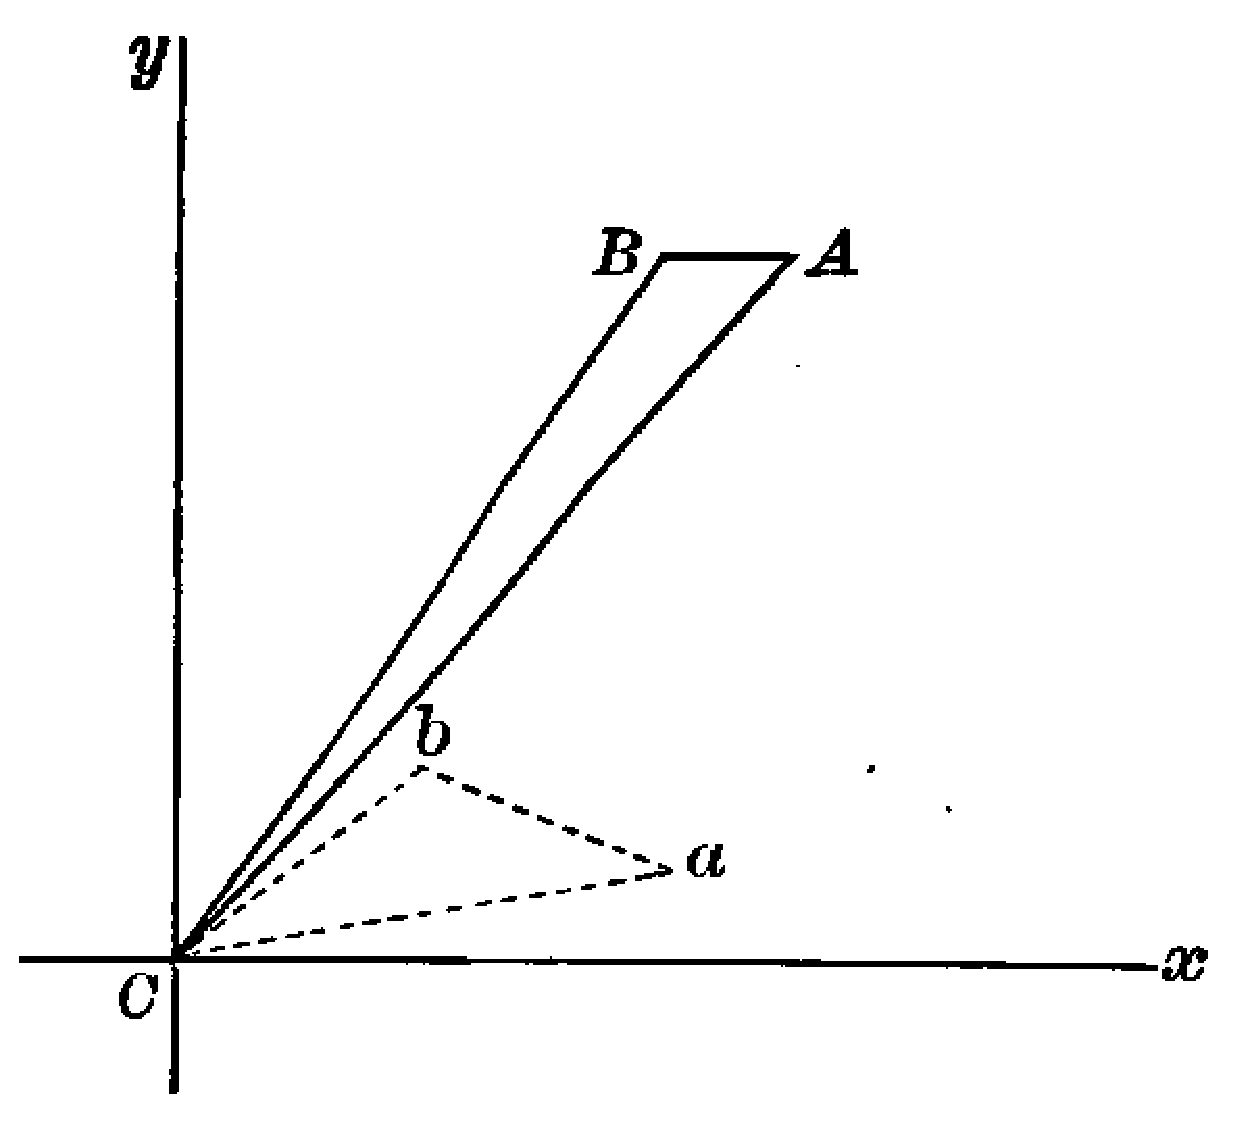
\includegraphics[scale=0.5]{images/Figure1.pdf}
\end{center}

\emph{Thus the area $\Delta$ of the triangle $ABC$ remains
unchanged} under a transformation of determinant unity and is an
invariant of the transformation. The triangle itself is not an
invariant, but is carried into $abC$. The area $\Delta$ is called
an \emph{absolute} invariant \index{absolute covariants} if $D =
1$. If $D \neq l$, all triangles having a vertex at the origin
will have their areas multiplied by the same number $D^{-1}$ under
the transformation. In such a case $\Delta$ is said to be a
\emph{relative} invariant. The adjoining figure illustrates the
transformation of $A(5,6)$, $B(4,6)$, $C(0,0)$ by means of

$$
x = x' + y', y = x' + 2y'.
$$

\subsection{An invariant ratio.}
In I the points (elements) of the
transformed system are located by means of two lines of
reference, and consist of the totality of points in a plane. For
a second illustration we consider the system of all points on
a line $EF$.

\begin{center}
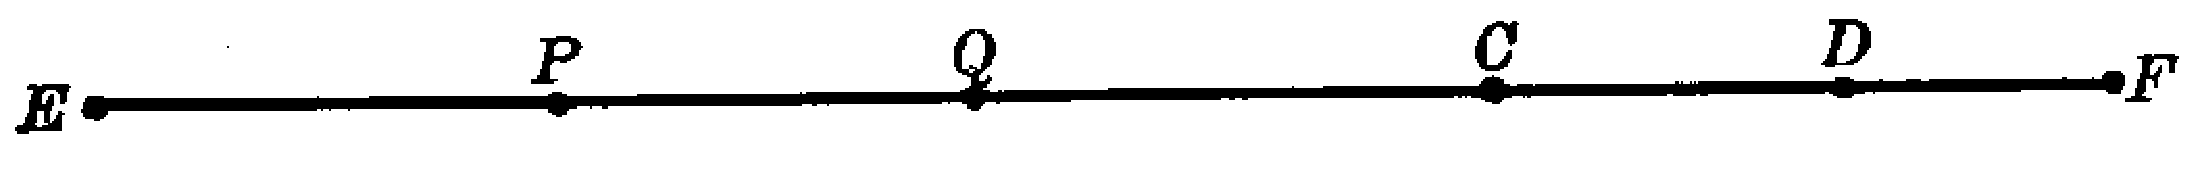
\includegraphics[scale=0.25]{images/Figure2.pdf}
\end{center}

We locate a point $C$ on this line by referring it to two fixed
points of reference $P, Q$. Thus $C$ will divide the segment $PQ$
in a definite ratio. This ratio,
\[
PC/CQ,
\]
is unique, being positive for points $C$ of internal division and
negative for points of external division. The point $C$ is said to
have for coordinates any pair of numbers $(x_{1},x_{2})$ such that
\begin{displaymath}
\lambda\frac{x_{1}}{x_{2}} = \frac{PC}{CQ}, \tag{2}
\end{displaymath}
where $\lambda$ is a multiplier which is constant for a given pair of
reference points $P, Q$. Let the segment $PC$ be positive and
equal to $\mu$. Suppose that the point $C$ is represented by the
particular pair $(p_{1}, p_{2})$, and let $D(q_{1}, q_{2})$ be any other point.
Then we can find a formula for the length of $CD$. For,

$$
\frac{CQ}{p_{2}} = \frac{PC}{\lambda p_{1}} = \frac{PQ}{\lambda p_{1} + p_{2}} = \frac{\mu}{\lambda p_{1} +p_{2}},
$$
and

$$
\frac{DQ}{q_{2}} = \frac{\mu}{\lambda q_{1} + q_{2}}.
$$
Consequently

\begin{displaymath}
CD = CQ = DQ = \frac{\lambda \mu (qp)}{(\lambda q_{1}
+q_{2})(\lambda p_{1} + p_{2})}. \tag{3}
\end{displaymath}

\newtheorem*{Theorem}{Theorem}
\index{Anharmonic ratio}
\begin{Theorem}The anharmonic ratio \{$CDEF$\} of four points
$C(p_{2}, p_{2})$, $D(q_{1}, q_{2})$, $E(r_{1}, r_{2})$, $F(\delta _{1}, \delta _{2})$, defined by

$$
\{CDEF\} = \frac{CD \cdot EF}{CF \cdot ED}.
$$
is an invariant under the general linear transformation

\begin{displaymath}
T : x_{1} = \lambda_{1}x'_{1} + \mu_{1}x'_{2}, x_{2} = \lambda_{2}x'_{1} + \mu_{2}x'_{2}, (\lambda \mu)\neq 0. \tag{$3_1$}
\end{displaymath}
\end{Theorem}

In proof we have from (3)

$$
\{CDEF\} = \frac{(qp)(\delta r)}{(\delta p)(qr)}.
$$
But under the transformation (cf. (1)),

\begin{displaymath}
(qp) = (\lambda \mu)(q'p'), \tag{4}
\end{displaymath}
and so on. Also, $C, D, E, F$ are transformed into the points
\[
  C'(p'_1, p'_2), D'(q'_1, q'_2), E'(r'_1, r'_2), F'(s'_1, s'_2),
\]
respectively. Hence
\[
  \{CDEF\} = \frac{(q p) (s r)}{(s p) (q r)}
           = \frac{(q' p') (s' r')}{(s' p') (q' r')}
           = \{C' D' E' F'\},
\]
and therefore the anharmonic ratio is an absolute invariant.

\subsection{An invariant discriminant.} \index{Discriminant}
A homogeneous quadratic
polynomial,
\[
  f = a_0 x^2_1 + 2 a_1 x_1 x_2 + a_2 x^2_2,
\]
when equated to zero, is an equation having two roots which
are values of the ratio $x_1/x_2$. According to II we may represent
these two ratios by two points $C(p_1, p_2), D(q_1, q_2)$ on
the line $EF$. Thus we may speak of the roots $(p_1, p_2),
(q_1, q_2)$ of $f$.

These two points coincide if the discriminant of $f$ vanishes,
and conversely; that is if
\[
  D = 4(a_0 a_2 - a^2_1) = 0
\]

If $f$ be transformed by $T$, the result is a quadratic polynomial
in $x'_1, x'_2$, or
\[
  f' = a'_0 x^{\prime 2}_1 + 2 a'_1 x'_1 x'_2 + a'_2 x^{\prime 2}_2,
\]

Now if the points $C, D$ coincide, then the two transformed points
$C', D'$ also coincide. For if $CD = 0$, (3) gives $(qp) = 0$.
Then (4) gives $(q' p') = 0$, since by hypothesis $(\lambda\mu)
\neq 0$. Hence, as stated, $C' D' = 0$.

It follows that the discriminant $D'$ of $f'$ must vanish as a
consequence of the vanishing of $D$. Hence
\[
  D' = K D.
\]

The constant $K$ may be determined by selecting in place
of $f$ the particular quadratic $f_1 = 2 x_1 x_2$ for which $D = -4$.
Transforming $f_1$ by $T$ we have
\[
  f'_1 = 2 \lambda_1 \lambda_2 x_1^2
         + 2 (\lambda_1 \mu_2 + \lambda_2 \mu_1) x_1 x_2
         + 2 \mu_1 \mu_2 x_2^2;
\]
and the discriminant of $f'_1$ is $D'=-4(\lambda\mu)^2$. Then the substitution
of these particular discriminants gives

\begin{align*}
-4(\lambda\mu)^2&=-4 K,\\
K &= (\lambda\mu)^2.
\end{align*}

We may also determine $K$ by applying the transformation $T$
to $f$ and computing the explicit form of $f'$. We obtain

\begin{align*}
a'_0 &= a_0\lambda_1^2+2 a_1\lambda_1\lambda_2+a_2\lambda^2_2,\\
a'_1 &= a_0\lambda_1\mu_1+a_1(\lambda_1\mu_2+\lambda_2\mu_1)+a_2\lambda_2\mu_2, \tag{5}\\
a'_2 &= a_0\mu_1^2+2a_1\mu_1\mu_2+a_2\mu_2^2,
\end{align*}
and hence by actual computation,

\[
4(a'_0 a'_2-a'^2_1) = 4(\lambda\mu)^2 (a_0 a_2-a_1^2),
\]
or, as above,

\[
D'=(\lambda\mu)^2D.
\]
Therefore the discriminant of $f$ is a relative invariant of $T$
(Lagrange 1773); and, in fact, the discriminant of $f'$ is
always equal to the discriminant of $f$ multiplied by the
square of the determinant of the transformation..

\subsubsection*{Preliminary Geometrical Definition.}
If there is associated with a geometric figure a quantity which is
left unchanged by a set of transformations of the figure, then
this quantity is called an absolute invariant of the set
(Halphen). In I the set of transformations consists of all linear
transformations for which $(\lambda\mu) = 1.$ In II and III the
set consists of all for which $(\lambda\mu) \neq 0$.

\subsection{An Invariant Geometrical Relation.}
Let the roots of
the quadratic polynomial $f$ be represented by the points
$(p_1,p_2),(r_1,r_2)$, and let $\phi$ be a second polynomial,

\[
\phi = b_0x_1^2 + 2b_1x_1x_2 + b_2x_2^2,
\]
whose roots are represented by $(q_1,q_2)$, $(s_1,s_2)$, or, in a
briefer notation, by $(q)$, $(s)$. Assume that the anharmonic
ratio of the four points $(p)$, $(q)$, $(r)$, $(s)$, equals minus one,
\[
\frac{(qp)(sr)}{(sp)(qr)}=-1
\tag{6}
\]
The point pairs $f=0, \phi=0$ are then said to be harmonic
conjugates. \index{Harmonically conjugate}We have from (6)
\[
2h \equiv 2p_2r_2s_1q_1 + 2p_1r_1s_2q_2 - (p_1r_2 + p_2r_1)(q_1s_2 + q_2s_1) = 0.
\]
But

\begin{align*}
& f = (x_1p_2 - x_2p_1)(x_1r_2-x_2r_1),\\
& \phi = (x_1q_2 - x_2q_1)(x_1s_2 - x_2s_1).
\end{align*}
Hence

\begin{align*}
& a_0 = p_2, \quad 2a_1 = -(p_2r_1 + p_1r_2), \quad a_2 = p_1r_1,\\
& b_0 = q_2s_2, \quad 2b_1 = - (q_2s_1 + q_1s_2), \quad b_2 =
q_1s_1,
\end{align*}
and by substitution in $(2h)$ we obtain

\[
h \equiv a_0b_2 -2a_1b_1 + a_2b_0 = 0.
\tag{7}
\]
That $h$ is a relative invariant under $T$ is evident from (6):
for under the transformation $f$, $\phi$ become, respectively,

\begin{align*}
& f'=(x'_1p'_2 - x'_2p'_1)(x'_1r'_2 - x'_2r'_1),\\
& \phi' =(x'_1q'_2 - x'_2q'_1)(x'_1s'_2 - x'_2s'_1),
\end{align*}
where

\begin{align*}
& p'_1 = \mu_2p_1 - \mu_1p_2, \quad p'_2 = -\lambda_2p_1 + \lambda_1p_2, \\
& r'_1 = \mu_2r_1 - \mu_1r_2, \quad r'_2 = -\lambda_2r_1 +
\lambda_1r_2,
\end{align*}
Hence

\[
(q'p')(s'r') + (s'p')(q'r') = (\lambda \mu)^2[(qp)(sr) + (sp)(qr)].
\]
That is,

\[
h' = (\lambda \mu)^2h.
\]

\emph{Therefore the bilinear function $h$ of the coefficients of two
quadratic polynomials, representing the condition that their
root pairs be harmonic conjugates, is a relative invariant of the
transformation $T$.} It is sometimes called a joint invariant,
or simultaneous invariant of the two polynomials under the
transformation.

\subsection{An invariant polynomial.}
To the pair of polynomials
$f, \phi$, let a third quadratic polynomial be adjoined,

\begin{align*}
\psi  & = c_0x^2_1 + 2c_1x_2x_2 + c_2x^2_2 \\
& =(x_1u_2 - x_2u_1)(x_1v_2 - x_2v_1).
\end{align*}
Let the points $(u_1, u_2)$ $(v_1,v_2)$, be harmonic conjugate to the
pair $(p)$, $(r)$; and also to the pair $(q)$, $(s)$. Then
\begin{align*}
c_0a_2-2c_1a_1-c_2a_0=&0,\\
c_0b_2-2c_1b_1-c_2b_0=&0,\\
c_0x_1^2+2c_1x_1x_2+c2x_2^2=&0.
\end{align*}
Elimination of the $c$ coefficients gives
\begin{equation}
  C=\begin{vmatrix}
      a_0&a_1&a_2\\
      b_0&b_1&b_2\\
      x_2^2&-x_1x_2 & x_1^2 \\
    \end{vmatrix} = 0 \tag{8}
\end{equation}
This polynomial,
\[
C=(a_0b_1-a_1b_0)x_1^2+(a_0b_2-a_2b_0)x_1x_2+(a_1b_2-a_2b_1)x_2^2,
\]
is the one existent quadratic polynomial whose roots form
a common harmonic conjugate pair, to each of the pairs $f$, $\phi$.

We can prove readily that $C$ is an invariant of the transformation
$T$. For we have in addition to the equations (5),
\begin{align*}
    b'_0&=b_0\lambda_1^2+2b_1\lambda_1\lambda_2+b_2\lambda_2^2,\\
    b'_1&=b_0\lambda_1\mu_1+b_1(\lambda_1\mu_2+\lambda_2\mu_1)
       +b_2\lambda_2\mu_2, \tag{9}\\
    b'_2&=b_0\mu_1^2+2b_1\mu_1\mu_2+b_2\mu_2^2.
\end{align*}
Also if we solve the transformation equations $T$ for $x'_1$, $x'_2$ in
terms of $x_1$, $x_2$ we obtain
\begin{align*}
    x'_1&=(\lambda\mu)^{-1}(\mu_2x_1-\mu_1x_2),\\
    x'_2&=(\lambda\mu)^{-1}(-\lambda_2x_1+\lambda_1x_2),\tag {10}\\
\end{align*}
Hence when $f$, $\phi$ are transformed by $T$, $C$ becomes
\begin{equation}
  \begin{array}[t]{l}
    C'= \\
    \{(a_0\lambda_1^2+2a_1\lambda_1\lambda_2+a_2\lambda_2^2)
    [b_0\lambda_1\mu_1+b_1(\lambda_1\mu_2+\lambda_2\mu_1)+b_2\lambda_2\mu_2]\\
    \ \ -(b_0\lambda_1^2+2b_1\lambda_1\lambda_2+b_2\lambda_2^2
      [a_0\lambda_1\mu_1+a_1(\lambda_1\mu_2+\lambda_2\mu_1)
                                        +a_2\lambda_2\mu_2]\}\\
    \ \ \times(\lambda\mu)^{-2}(\mu_2x_1-\mu_1x_2)^2+\cdots.\\
  \end{array} \tag {11}
\end{equation}
When this expression is multiplied out and rearranged as
a polynomial in $x_1$, $x_2$, it is found to be $(\lambda\mu)C$. That is,
\[
  C'=(\lambda\mu)C
\]
and therefore $C$ is an invariant.

It is customary to employ the term invariant to signify a function
of the coefficients of a polynomial, which is left unchanged, save
possibly for a numerical multiple, when the polynomial is
transformed by $T$. If the invariant function involves the
variables also, it is ordinarily called a \emph{covariant}. Thus
$D$ in III is a relative invariant, whereas $C$ is a relative
covariant.\index{Covariants!definition}

\subsubsection*{The Inverse of a Linear Transformation.}
The process (11) of proving by direct computation the invariancy
of a function we shall call \emph{verifying} the invariant or
covariant. The set of transformations (10) used in such a
verification is called the \emph{inverse} of $T$ and is denoted by
$T^{-1}$. \index{Groups:!of transformations}

\subsection{An invariant of three lines.}
Instead of the Cartesian co\"ordinates employed in I we may
introduce homogeneous variables $(x_1,x_2,x_3)$ to represent a
point $P$ in a plane. These variables may be regarded as the
respective distances of $N$ from the three sides of a triangle of
reference. Then the equations of three lines in the plane may be
written
\begin{align*}
a_{11}x_1+a_{12}x_2+a_{13}x_3&=0,\\
a_{21}x_1+a_{22}x_2+a_{23}x_3&=0,\\
a_{31}x_1+a_{32}x_2+a_{33}x_3&=0.\\
\end{align*}
The eliminant of these,
\[
D=\begin{vmatrix}
a_{11}&a_{12}&a_{13}\\
a_{21}&a_{22}&a_{23}\\
a_{31}&a_{32}&a_{33}\\
\end{vmatrix}
,
\]
evidently represents the condition that the lines be concurrent.
For the lines are concurrent if $D = 0$. Hence we
infer from the geometry that $D$ is an invariant, inasmuch as
the transformed lines of three concurrent lines by the following
transformations, $ S$, are concurrent:
\begin{equation}
S:
\begin{array}[c]{l}
x_1=\lambda_1x'_1+\mu_1x'_2+\nu_1x'_3,\\
x_2=\lambda_2x'_1+\mu_2x'_2+\nu_2x'_3,\\
x_1=\lambda_3x'_1+\mu_3x'_2+\nu_3x'_3.\\
\end{array}
\ \ (\lambda\mu\nu)\neq 0. \tag{12}\end{equation} To verify
algebraically that $D$ is an invariant we note that the
transformed of
\[
a_{i1}x_1 + a_{i2}x_2 + a_{i3}x_3 \quad (i = 1,2,3),
\]
by $S$ is
\begin{align*}
(a_{i1}\lambda_1 + a_{i2}\lambda_2 +& a_{i3}\lambda_3)x'_1 +
(a_{i1}\mu_1 + a_{i2}\mu_2 + a_{i3}\mu_3)x'_2 + (a_{i1}v_1 \\
+ & a_{i2}v_2 + a_{i3}v_3)x'_3 \quad (i = 1,2,3). \tag{13}
\end{align*}

Thus the transformed of $D$ is

\begin{align*}
D' &= \begin{vmatrix}
a_{11}\lambda_1 + a_{12}\lambda_2 + a_{13}\lambda_3 &
a_{11}\mu_1 + a_{12}\mu_2 + a_{13}\mu_3 &
a_{11}\nu_1 + a_{12}\nu_2 + a_{13}\nu_3 \\
a_{21}\lambda_1 + a_{22}\lambda_2 + a_{23}\lambda_3 &
a_{21}\mu_1 + a_{22}\mu_2 + a_{23}\mu_3 &
a_{21}\nu_1 + a_{22}\nu_2 + a_{23}\nu_3 \\
a_{31}\lambda_1 + a_{32}\lambda_2 + a_{33}\lambda_3 &
a_{31}\mu_1 + a_{32}\mu_2 + a_{33}\mu_3 &
a_{31}\nu_1 + a_{32}\nu_2 + a_{33}\nu_3
\end{vmatrix} \\
 &= (\lambda\mu\nu)D.
\tag{14}\end{align*}
The latter equality holds by virtue of the ordinary law of the
product of two determinants of the third order. Hence $D$ is
an invariant.

\subsection{A Differential Invariant.} \index{Differential
invariant} \index{Transformations, non-linear} In previous
illustrations the transformations introduced have been of the
linear homogeneous type. Let us next consider a type of
transformation which is not linear, and an invariant which
represents the differential of the arc of a plane curve or simply
the distance between two consecutive points $(x, y)$ and $(x + dx,
y + dy)$ in the $(x, y)$ plane.

We assume the transformation to be given by

\[
x' = X(x, y, a), \quad y' = Y(x, y, a),
\]
where the functions $X$, $Y$ are two independent continuous
functions of $x$, $y$ and the parameter $a$. We assume $(a)$ that
the partial derivatives of these functions exist, and $(b)$ that
these are continuous. Also $(c)$ we define $X$, $Y$ to be such
that when $a = a_0$

\[
X(x, y, a_0) = x, \ Y(x. y, a_0) = y.
\]
Then let an increment $\delta a$ be added to $a_0$ and expand each
function as a power series in $\delta a$ by Taylor's theorem. This
gives

\begin{align*}
x' &= X(x, y, a_0) + \frac{\partial X(x,y,a_0)} {\partial a_0} \delta a + \ldots,\\
y' &= Y(x, y, a_0) + \frac{\partial Y(x,y,a_0)} {\partial a_0} \delta a + \ldots. \tag{15}
\end{align*}
Since it may happen that some of the partial derivatives of
$X$, $Y$ may vanish for $a = a_0$, assume that the lowest power
of $\delta a$ in (15) which has a non-vanishing coefficient is $(\delta a)^k$,
and write $(\delta a)^k = \delta t$. Then the transformation, which is infinitesimal,
becomes

\[
I: \ \begin{matrix}
x' = x + \xi \delta t, \\
y' = y + \eta \delta t.
\end{matrix}
\]
where $\xi$, $\eta$ are continuous functions of $x$, $y$. The
effect of operating $I$ upon the co\"ordinates of a point $P$ is
to add infinitesimal increments to those co\"ordinates, viz.
\begin{align*}
\delta x = \xi \delta t, \\
\delta y = \eta \delta t.
\tag{16}\end{align*}
Repeated operations with $I$ produce a continuous motion
of the point $P$ along a definite path in the plane. Such a
motion may be called a stationary streaming in the plane
(Lie).

Let us now determine the functions $\xi$, $\eta$, so that
\[
\sigma = dx^2 + dy^2
\]
shall be an invariant under $I$.

By means of $I$, $\sigma$ receives an infinitesimal increment $\delta \sigma$.
In order that $\sigma$ may be an absolute invariant, we must have

\[
\frac{1}{2} \delta \sigma = dx\delta dx + dy\delta dy = 0,
\]
or, since differential and variation symbols are permutable,
\[
dxd \delta x + dyd \delta y = dxd \xi + dyd \eta =0.
\]
Hence
\[
(\xi_x dx + \xi_y dy) dx + (\eta_x dx + \eta_y dy) dy = 0.
\]
Thus since $dx$ and $dy$ are independent differentials
\[
\xi_x = \eta_y = 0, \quad \xi_y + \eta_x = 0.
\]
That is, $\xi$ is free from $x$ and $\eta$ from $y$. Moreover
\[
\xi_{xy} = \eta_{xx} = \xi_{yy} = 0.
\]
Hence $\xi$ is linear in $y$, and $\eta$ is linear in x; and also from
\begin{align*}
\xi_y &= - \eta_x, \\
\xi &= \alpha y + \beta, \quad \eta = - \alpha x + \gamma.
\tag{17}
\end{align*}
Thus the most general infinitesimal transformation leaving
$\sigma$ invariant is
\begin{equation}
I: x' = x + (\alpha y + \beta) \delta t, \quad y' = y + (-\alpha x
+ \gamma) \delta t. \tag{18}\end{equation} Now there is one point
in the plane which is left invariant, viz.
\[
x = \gamma / \alpha, \quad y = - \beta / \alpha.
\]
The only exception to this is when $\alpha = 0$. But the transformation
is then completely defined by
\[
x' = x + \beta \delta t, \quad y' = y + \gamma \delta t,
\]
and is an infinitesimal translation parallel to the co\"ordinate
axes. Assuming then that $\alpha \neq 0$, we transform
co\"ordinate axes so that the origin is moved to the invariant
point. This transformation,
\[
x = x + \gamma / \alpha, \quad y = y - \beta / \alpha,
\]
leaves $\sigma$ unaltered, and $I$ becomes
\begin{equation}
x' =x + \alpha y \delta t, \quad y' = y - \alpha x \delta t.
\tag{19}\end{equation} But (19) is simply an infinitesimal
rotation around the origin. We may add that the case $\alpha = 0$
does not require to be treated as an exception since an
infinitesimal translation may be regarded as a rotation around the
point at infinity. Thus,

\begin{Theorem}The most general infinitesimal transformation
which leaves $\sigma = dx^2 + dy^2$ invariant is an infinitesimal rotation
around a definite invariant point in the plane.
\end{Theorem}

We may readily interpret this theorem geometrically by
noting that if $\sigma$ is invariant the motion is that of a rigid
figure. As is well known, any infinitesimal motion of a plane
rigid figure in a plane is equivalent to a rotation around a
unique point in the plane, called the instantaneous center.
The invariant point of $I$ is therefore the instantaneous center
of the infinitesimal rotation.

\begin{center}
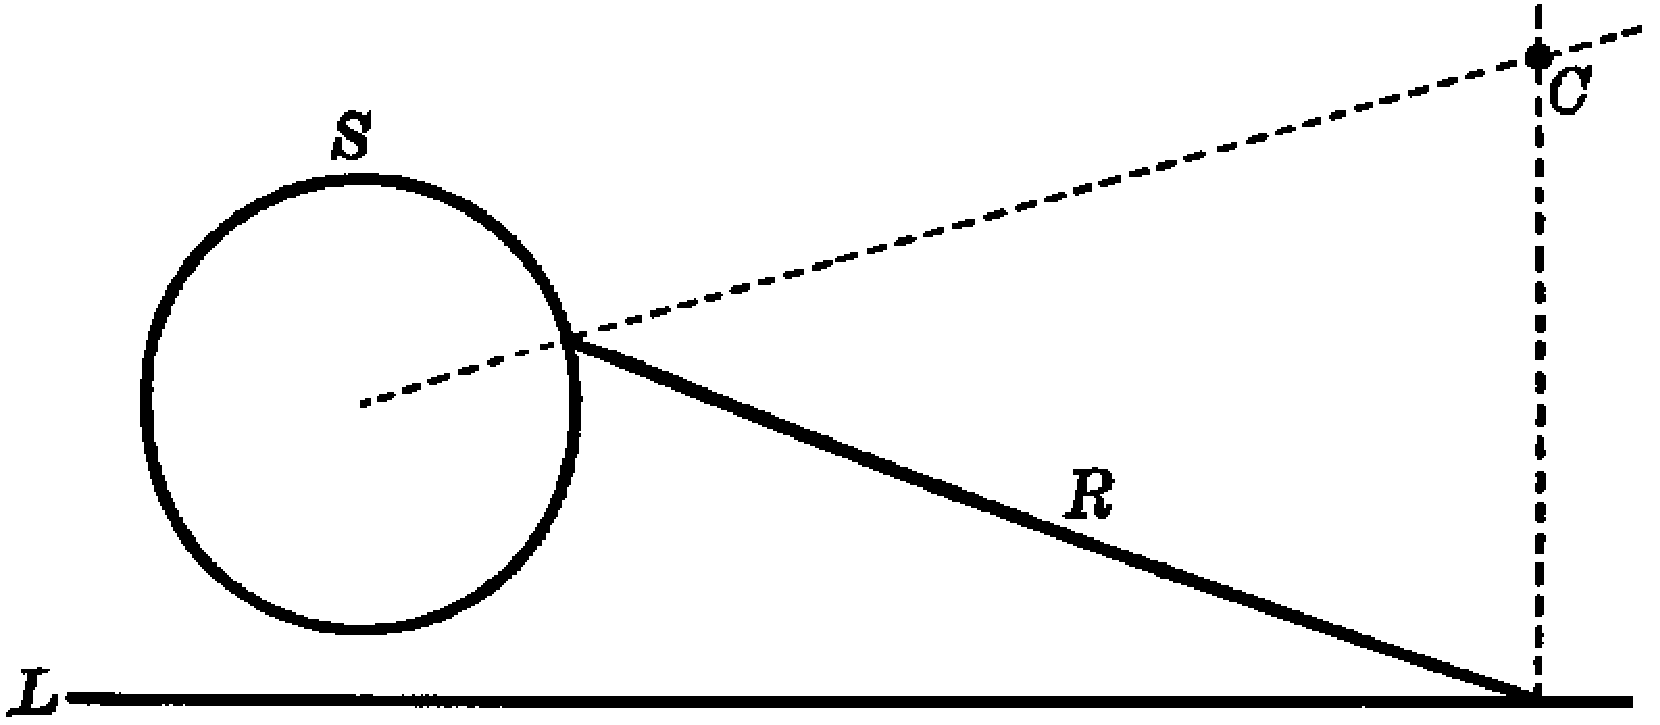
\includegraphics[scale=0.3]{images/Figure3.pdf}
\end{center}

The adjoining
figure shows the
invariant point
($C$) when the
moving figure is
a rigid rod $R$ one
end of which slides on a circle $S$, and the other along a
straight line $L$. This point is the intersection of the radius
produced through one end of the rod with the perpendicular
to $L$ at the other end.

\subsection{An Arithmetical Invariant.} \index{Arithmetical
invariants} \index{Modular:!transformation} Finally let us
introduce a transformation of the linear type like

\[
T: x_l = \lambda_1x'_1 + \mu_1x'_2, \ x_2 = \lambda_2x'_1 + \mu_2x'_2,
\]
but one in which the coefficients $\lambda, \mu$ are positive integral
residues of a prime number $p$. Call this transformation $T_p$.
We note first that $T_p$ may be generated by combining the
following three particular transformations:
\begin{align*}
(a) \ x_1 &= x'_1 + tx'_2, \ x_2 = x'_2,\\
(b) \ x_1 &= x'_1, \ x_2 = \lambda x'_2, \tag{20}\\
(c) \ x_1 &= x'_2, \ x_2 = -x'_1,
\end{align*}
where $t$, $\lambda$ are any integers reduced modulo $p$. For $(a)$
repeated gives
\begin{equation*}
x_1 = (x''_1 + tx''_2) + tx''_2 = x''_1 + 2 tx''_2, \ x_2 = x''_2.
\end{equation*}
Repeated $r$ times $(a)$ gives, when $rt \equiv u$ (mod $p$),
\begin{equation*}
(d) \; x_1 = x'_1 + ux'_2, \ x_2 = x'_2.
\end{equation*}
Then $(c)$ combined with $(d)$ becomes
\begin{equation*}
(e) \; x_1 = -ux'_1 + x'_2, \ x_2 = -x'_1.
\end{equation*}
Proceeding in this way $T_p$ may be built up.

Let
\begin{equation*}
f = a_0x^2_1 + 2a_1x_1x_2 + a_2x^2_2,
\end{equation*}
where the coefficients are arbitrary variables; and
\begin{equation}
g = a_0x^4_1 + a_1 ( x^3_1x_2 + x_1x^3_2 ) + a_2x^4_2,
\tag{21}
\end{equation}
and assume $p = 3$. Then we can prove that $g$ is an arithmetical
covariant; in other words a covariant modulo 3.
This is accomplished by showing that if $f$ be transformed
by $T_3$ then $g'$ will be identically congruent to $g$ modulo 3.
When $f$ is transformed by $(c)$ we have
\begin{equation*}
f' = a_2x'^2_1 - 2 a_1x'_1x'_2 + a_0x'^2_2.
\end{equation*}
That is,
\begin{equation*}
a'_0 = a_2, \ a'_1 = -a_1, \ a'_2 = a_0.
\end{equation*}
The inverse of $(c)$ is $x'_2 = x_1, \ x'_1 = -x_2$. Hence
\begin{equation*}
g' = a_2x^4_2 + a_1 (x_1x^3_2 + x_1^3x_2) + a_0x^4_1 = g,
\end{equation*}
and $g$ is invariant, under $(c)$.

Next we may transform $f$ by $(a)$; and we obtain
\begin{equation*}
a'_0 = a_0, \ a'_1 = a_0t + a_1, \ a'_2 = a_0t^2 + 2a_1t + a_2.
\end{equation*}
The inverse of $(a)$ is
\begin{equation*}
x'_2 = x_2, \ x'_1 = x_1 - tx_2.
\end{equation*}
Therefore we must have
\begin{align*}
g' = a_0(x_1 - tx_2)^4  &+  (a_0t + a_1)\left[(x_1 - tx_2)^3x_2 + (x_1 - tx_2)x^3_2 \right] \\
&+ (a_0t^2 + 2a_1t + a_2)x^4_2 \tag{22} \\
&\equiv a_0x^4_1 + a_1 (x^3_1x_2 + x_1x^3_2) + a_2x^4_2 \: (\textrm{mod 3}) \\
\end{align*}
But this congruence follows immediately from the following case of
Fermat's theorem:\index{Fermat's theorem}
\[
t^3 \equiv t (\text{mod } 3).
\]
Likewise $g$ is invariant with reference to \emph{(b)}. Hence $g$ is
a formal modular covariant of $f$ under $T_3$.

\section{Terminology and Definitions. Transformations}
We proceed to formulate some definitions upon which
immediate developments depend.

\subsection{An invariant.}
Suppose that a function of $n$ variables,
$f$, is subjected to a definite set of transformations upon
those variables. Let there be associated with $f$ some definite
quantity $\phi$ such that when the corresponding quantity
$\phi'$ is constructed for the transformed function $f'$ the equality
\[
\phi' = M\phi
\]
holds. Suppose that $M$ depends only upon the transformations,
that is, is free from any relationship with $f$. Then $\phi$
is called an invariant of $f$ under the transformations of the set.

The most extensive subdivision of the theory of invariants
in its present state of development is the theory of invariants
of algebraical polynomials under linear transformations.
Other important fields are differential invariants and number-theoretic
invariant theories. In this book we treat, for
the most part, the algebraical invariants.

\subsection{Quantics or forms.}
A homogeneous polynomial in $n$
variables $ x_1, x_2, \dots, x_n $ of order $m$ in those variables is called a
\emph{quantic}, or \emph{form}, of order $m$. Illustrations are
\begin{align*}
f(x_1, x_2) &= a_0x_1^3 + 3 a_1x_1^2x_2 + 3a_2x_1x_2^2 + a_3x_2^3,\\
f(x_1, x_2, x_3) &= a_{200}x_1^2 + 2a_{110}x_1x_2 + a_{020}x_2^2 +
2a_{101}x_1x_3 + 2a_{011}x_2x_3 + a_{002}x_3^2
\end{align*}
With reference to the number of variables in a quantic it is called binary, ternary; and if there are $n$ variables,
$n$-ary. Thus $f(x_1, x_2)$ is a binary cubic form; $f(x_1, x_2, x_3)$ a
ternary quadratic form. In algebraic invariant theories of
binary forms it is usually most convenient to introduce with
each coefficient $a_i$ the binomial multiplier $\binom{m}{i}$ as in $f(x_1, x_2)$.
When these multipliers are present, a common notation for a
binary form of order $m$ is (Cayley)

$$
f(x_1, x_2) = (a_0, a_1, \cdots, a_m \between x_1,x_2)^m =
a_0x_1^m + ma_1x_1^{m-1}x_2 + \cdots.
$$
If the coefficients are written without the binomial numbers,
we abbreviate

$$
f(x_1, x_2) = (a_0, a_1, \cdots, a_m \between x_1, x_2)^m =
a_ax_1^m + a_1x_1^{m-1}x_2 + \cdots.
$$
The most common notation for a ternary form of order $m$ is
the generalized form of $f(x_1, x_2, x_3)$ above. This is

$$
f(x_1,x_2,x_3) = \sum_{p,q,r=0}^m
\frac{m!}{p!q!r!}
a_{pqr}x_1^px_2^qx_3^r,
$$
where $p, q, r$ take all positive integral values for which $p + q
+ r = m$. It will be observed that the multipliers associated with
the coefficients are in this case multinomial numbers. Unless the
contrary is stated, we shall in all cases consider the
coefficients $a$ of a form to be arbitrary variables. As to
coordinate representations we may assume $(x_1, x_2, x_3)$, in a
ternary form for instance, to be homogenous co\"ordinates of a
point in a plane, and its coefficients $a_{pqr}$ to be homogenous
coordinates of planes in $M$-space, where $M+1$ is the number of
the $a$'s. Thus the ternary form is represented by a point in $M$
dimensional space and by a curve in a plane. \index{Co\"ordinates}

\subsection{Linear Transformations.}\index{Linear transformations}
The transformations to which the variables in an $n$-ary form will
ordinarily be subjected are the following linear transformations
called collineations:\index{Transformed form:!binary}
\begin{align*}
x_1 &=\lambda_1x'_1+\mu_1x'_2+ \ldots +\sigma_1x'_n \\
x_2 &=\lambda_2x'_1+\mu_2x'_2+ \ldots +\sigma_2x'_n \tag{23}\\
&\ldots \\
x_n &=\lambda_nx'_1+\mu_nx'_2+ \ldots +\sigma_nx'_n.\\
\end{align*}
In algebraical theories the only restriction to which these
transformations will be subjected is that the inverse transformation
shall exist. That is, that it be possible to solve for
the primed variables in terms of the un-primed variables (cf.
(10)). We have seen in Section 1, V (11), and VIII (22)
that the verification of a covariant and indeed the very existence
of a covariant depends upon the existence of this inverse
transformation.

\begin{Theorem}A necessary and sufficient condition in order
that the inverse of (23) may exist is that the determinant or
modulus of the transformation,
\[
M=(\lambda\mu\nu \ldots \sigma)=\begin{vmatrix}
\lambda_1, &  \mu_1,  & \nu_1, & \ldots & \sigma_1\\
\lambda_2, &  \mu_2,  & \nu_2, & \ldots & \sigma_2\\
\vdots & \vdots & \vdots & \ddots & \vdots\\
\lambda_n, &  \mu_n,  & \nu_n, & \ldots & \sigma_n\\
\end{vmatrix},
\]
shall be different from zero.\end{Theorem}

In proof of this theorem we observe that the minor of any
element, as of $\mu_i$, of $M$ equals $\frac{\partial M}{\partial \mu_i}$. Hence, solving for a
variable as $x'_2$, we obtain
\[
x'_2=M^{-1}\left(x_1\frac{\partial M}{\partial \mu_1}+x_2\frac{\partial M}{\partial \mu_2}+ \ldots +x_n\frac{\partial M}{\partial \mu_n}\right),
\]
and this is a defined result in all instances except when
$M=0$, when it is undefined. Hence we must have $M\neq0$.

\subsection{A theorem on the transformed polynomial.}
Let $f$ be a
polynomial in $x_1, x_2$ of order $m$,
\[
f(x_1,x_2)=a_0x_1^m+ma_1x_1^{m-1}x_2+\binom{m}{2}a_2x_1^{m-2}x_2^2+ \ldots +a_mx_2^m.
\]
Let $f$ be transformed into $f'$ by $T$ (cf. $3_{1}$)
\[
f' = a'_{0} x'^{m}_{1} + ma'_{1} x'^{m-1}_{1} x'_{2} + \cdots + \binom{m}{r} a'_{r} x'^{m-r}_{1} x'^{r}_{2} + \cdots + a'_{m}  x'^{m}_{2}.
\]

We now prove a theorem which gives a short method of
constructing the coefficients $a'_r$ in terms of the coefficients
$a_{0}, \ldots, a_{m}$.

\begin{Theorem}The coefficients $a'_{r}$ of the transformed form $f'$ are
given by the formulas
\begin{align*}
a'_{r}=\frac{(m-r)!}{m!}
\left(\mu_{1}\frac{\partial}{\partial\lambda_{1}} + \mu_{2}
\frac{\partial}{\partial\lambda_{2}}\right)^{r}
f(\lambda_{1},\lambda_{2}) \quad (r=0,\ldots,m). \tag{$23_1$}
\end{align*}
\end{Theorem}

In proof of this theorem we note that one form of $f'$ is
$f(\lambda_{1}x'_{1}+\mu_{1}x'_{2}, \lambda_{2}x'_{1}+\mu_{2}x'_{2})$. But since $f'$ is homogeneous this
may be written
$$
f'=x'^{m}_{1} f(\lambda_{1}+\mu_{1}x'_{2}/x'_{1}, \lambda_{2} + \mu_{2}x'_{2}/x'_{1}).
$$
We now expand the right-hand member of this equality by
Taylor's theorem, regarding $x'_2/x'_1$ as a parameter,

\begin{align*}
f' &= x'^{m}_{1}\left[ f(\lambda_{1},\lambda_{2}) + \frac{x'_2}{x'_1} \left(\mu \frac{\partial}{\partial \lambda}\right) f (\lambda_{1},\lambda_{2}) \right. \\
&  +\frac{1}{2!} \left(\frac{x'_2}{x'_1}\right)^2 \left(\mu \frac{\partial}{\partial\lambda}\right)^2 f(\lambda_{1},\lambda_{2})+ \cdots \\
&+ \left. \frac{1}{r!} \left(\frac{x'_2}{x'_1}\right)^r \left(\mu
\frac{\partial}{\partial\lambda}\right)^r f(\lambda_1,\lambda_2) +
\cdots \right],
\end{align*}
where
\begin{align*}
\left(\mu \frac{\partial}{\partial\lambda}\right) &= \left(\mu_{1} \frac{\partial}{\partial\lambda_{1}} + \mu_{2} \frac{\partial}{\partial\lambda_{2}}\right),\\
f'=f(\lambda_1,\lambda_2) x'^m_1 + \cdots &+ \frac{1}{r!} \left(\mu \frac{\partial}{\partial\lambda}\right)^{r} f(\lambda_1,\lambda_2) x'^{m-r}_1 x'^{r}_{2} + \cdots \\
&+ \frac{1}{m!} \left(\mu
\frac{\partial}{\partial\lambda}\right)^m
f(\lambda_1,\lambda_2)x'^{m}_{2}.
\end{align*}
Comparison of this result with the above form of $f'$ involving
the coefficients $a'_r$ gives ($23_1$).

An illustration of this result may be obtained from (5).
Here $m = 2$, and

\begin{align*}
a'_0 &= a_0\lambda_1^2 + 2a_1\lambda_1\lambda_2 + a_2\lambda_2^2 = f(\lambda_1, \lambda_2) = f_0, \\
a'_1 &= a_0\lambda_1\mu_1 + a_1(\lambda_1\mu_2 + \lambda_2\mu_1) + a_2\lambda_2\mu_2 = \frac{1}{2}\left(\mu\frac{\partial}{\partial\lambda}\right)f(\lambda_1, \lambda_2), \tag{24} \\
a'_2 &= a_0\mu_1^2 + 2a_1\nu_1\mu_2 + a_2\mu_2^2 =
\frac{1}{2}\left(\mu
\frac{\partial}{\partial\lambda}\right)^2f(\lambda_1, \lambda_2).
\end{align*}

\subsection{A group of transformations.}
If we combine two transformations,
as $T$ and
\begin{align*}
T': \begin{matrix}
x'_1 = \xi_1x''_1 + \eta_1x''_2, \\
x'_2 = \xi_2x''_2 + \eta_2x''_2,
\end{matrix}
\end{align*}
there results
\begin{align*}
TT': \begin{matrix}
x_1 = (\lambda_1\xi_1 + \mu_1\xi_2)x''_1 + (\lambda_1\eta_1 + \mu_1\eta_2)x''_2, \\
x_2 = (\lambda_2\xi_1 + \mu_2\xi_2)x''_1 + (\lambda_2\eta_1 + \mu_2\eta_2)x''_2,
\end{matrix}
\end{align*}
This is again a linear transformation and is called the product
of $T$ and $T'$. If now we consider $\lambda_1, \lambda_2, \mu_1, \mu_2$ in $T$ to
be independent continuous variables assuming, say, all real
values, then the number of linear transformations is infinite,
\emph{i.e.} they form an infinite set, but such that the product of any
two transformations of the set is a third transformation of
the set. Such a set of transformations is said to form a
\emph{group}. The complete abstract definition of a group is the
following:

Given any set of distinct operations $T, T'', T''', \cdots$, finite or
infinite in number and such that:

($\alpha$) The result of performing successively any two operations
of the set is another definite operation of the set which
depends only upon the component operations and the sequence
in which they are carried out:

($\beta$) The inverse of every operation $T$ exists in the set;
that is, another operation $T^{-l}$ such that $TT^{-l}$ is the identity
or an operation which produces no effect.

This set of operations then forms a group.

The set described above therefore forms an infinite group.
If the transformations of this set have only integral coefficients
consisting of the positive residues of a prime number
$p$, it will consist of only a finite number of operations and so
will form a finite group.

\subsection{The induced group.}\index{Groups:!the induced
group}\index{Induced group} The equalities (24) constitute a set
of linear transformations on the variables $a_0, a_1, a_2$.
Likewise in the case of formulas ($23_1$). These transformations
are said to be \emph{induced} by the transformations $T$. If $T$
carries $f$ into $f'$ and $T''$ carries $f'$ into $f''$, then
\begin{align*}
a''_r &= \frac{(m-r)!}{m!} \left( \eta \frac{\partial}{\partial\xi} \right)^r f'(\xi_1,\xi_2)  \\
      &= \frac{(m-r)!}{m!} \left( \eta \frac{\partial}{\partial\xi} \right)
          \sum^m_{s=0}\frac{1}{s!} \left(\mu \frac{\partial}{\partial\lambda}\right)^s
          f(\lambda_1, \lambda_2) \xi^{m-2}_1\xi^s_2.
\tag{$24_1$} \\
(r = 0, 1, \cdots , m).
\end{align*}
This is a set of linear transformations connecting the $a''_r$
directly with $a_0, \cdots, a_m$. The transformations are induced
by applying $T$, $T''$ \emph{in succession} to $f$. Now \emph{the
induced transformations ($23_1$) form a group}; for the
transformations induced by applying $T$ and $T'$ in succession is
identical with the transformation induced by the product $TT'$.
This is capable of formal proof. For by ($28_1$) the result of
transforming $f$ by $TT'$ is
\begin{equation*}
a''_r = \frac{(m-r)!}{m!}\Delta^rf(\lambda_1\xi_1 + \mu_1\xi2, \lambda_2\xi_1 + \mu_2\xi_2),
\end{equation*}
where
\begin{equation*}
\Delta = (\lambda_1\eta_1 + \mu_1\eta_2) \frac{\partial}{\partial(\lambda_1\xi_1 + \mu_1\xi_2)}
 + (\lambda_2\eta_1 + \mu_2\eta_2) \frac{\partial}{\partial(\lambda_2\xi_1 + \mu_2\xi_2)}
\end{equation*}
But
\begin{align*}
(\lambda_1\eta_1+\mu_1\eta_2)&
 \frac{\partial}{\partial(\lambda_1\xi_1+\mu_1\xi_2)}\\
&=\eta_1 \frac{\partial}{(\lambda_1\xi_1+\mu_1\xi_2)}
\frac{\partial(\lambda_1\xi_1+\mu_1\xi_2)}{\partial\xi_1}\\
& +\eta_2 \frac{\partial}{(\lambda_1\xi_1+\mu_1\xi_2)}
\frac{\partial(\lambda_1\xi_1+\mu_1\xi_2)}{\partial\xi_2}\\
& = \eta_1\frac{\partial}{\partial\xi_1} +
\eta_2\frac{\partial}{\partial\xi_2}.
\end{align*}
Hence
\[
\Delta=\left(\eta\frac{\partial}{\partial\xi}\right )+
       \left(\eta\frac{\partial}{\partial\xi}\right )
\]
and by the method of (IV) combined with this value of $\Delta$
\[
a''_r=\frac{(m-r)!} {m!}
\left ( \eta\frac{\partial}{\partial \xi}\right )^r
\sum_0^m\frac {1} {s!}
\left ( \mu \frac{\partial}{\partial \lambda}\right )^s
f(\lambda_1,\lambda_2)\xi_1^{m-s}\xi_2^s.
\]
But this is identical with ($24_1$). Hence the induced transformations
form a group, as stated. This group will be
called the \emph{induced group}.

\subsubsection*{Definition.} A quantic or form, as for instance a binary
cubic $f$, is a function of two distinct sets of variables,
\emph{e.g.} the variables $x_1$, $x_2$, and the coefficients
$a_0,\dots,a_3$. It is thus quaternary in the coefficients and
binary in the variables $x_1,x_2$. We call it a quaternary-binary
function. In general, if a function $F$ is homogeneous and of
degree \index{Degree} $i$ in one set of variables and of order
$\omega$ in a second set, and if the first set contains $m$
variables and the second set $n$, then $F$ is said to be an
$m$-ary-$n$-ary function of \emph{degree-order} $(i,\omega)$. If
the first set of variables is $a_0,\dots,a_m$, and the second and
the second $x_1,\dots,x_n$, we frequently employ the notation
\[
F=(a_0,\dots,a_m)^i(x_1,\dots,x_n)^\omega.
\]

\subsection{Cogrediency.}\index{Cogrediency}
In many invariant theory problems two sets of variables are
brought under consideration simultaneously. If these sets $(x_1,
x_2, \cdots, x_n)$, $(y_1, y_2, \cdots, y_n)$ are subject to the
same scheme of transformations, as (23), they are said to be
cogredient sets of variables.

As an illustration of cogredient sets we first take the
modular binary transformations,
\[
T_p:x_1=\lambda_1x_1^{\prime}+\mu_1x_2^{\prime}, x_2=\lambda_2x_1^{\prime}+\mu_2x_2^{\prime},
\]
where the coefficients $\lambda,\mu$ are integers reduced modulo $p$ as
in Section 1, VIII. We can prove that with reference to
$T_p$ the quantities $x_1^p, x_2^p,$ are cogredient to $x_1, x_2$. For all
binomial numbers $\binom{p}{i}$, where $p$ is a prime, are divisible by
$p$ except $\binom{p}{0}$ and $\binom{p}{p}$. Hence, raising the equations of $T_p$ to
the $p$th power, we have
\[
x_1^p\equiv\lambda_1^px_1^{\prime p}+\mu_1^px_2^{\prime p},
x_2^p\equiv\lambda_2^px_1^{\prime p}+ \mu_2^px_2^{\prime p} \text{
(mod }p).
\]
But by Fermat's theorem, \index{Fermat's theorem}
\[
\lambda_i^p\equiv\lambda_i, \mu_i^p\equiv\mu_i \text{ (mod }p) \
(i=1, 2).
\]
Therefore
\[
x_1^p=\lambda_1x_1^{\prime p}+\mu_1x_2^{\prime p}, x_2^p=\lambda_2x_1^{\prime p}+\mu_2x_2^{\prime p},
\]
and the cogrediency of $x_1^p, x_2^p$ with $x_1, x_2$ under $T_p$ is proved.

\subsection{Theorem on the roots of a polynomial.}
\begin{Theorem}
The roots $(r_1^{(1)}, r_2^{(1)}), (r_1^{(2)}, r_2^{(2)}), \cdots,$
$((r_1^{(m)}, r_2^{(m)})$ of a binary form
\[
f=a_0x_1^m+ma_1x_1^{m-1}x_2+...+a_mx_2^m,
\]
are cogredient to the variables.
\end{Theorem}

To prove this we write
\[
f=(r_2^{(1)}x_1-r_1^{(1)}x_2)(r_2^{(2)}x_1-r_1^{(2)}x_2)\cdots(r_2^{(m)}x_1-r_1^{(m)}x_2),
\]
and transform $f$ by $T$.  There results
\[
f^{\prime}=\prod_{i=1}^m\left[(r_2^{(i)}\lambda_1-r_1^{(i)}\lambda_2)x_1^{\prime}+
(r_2^{(i)}\mu_1-r_1^{(i)}\mu_2)x_2^{\prime}\right].
\]
Therefore
\[
r_2^{\prime(i)}=r_2^{(i)}\lambda_1-r_1^{(i)}\lambda_2; \
r_1^{\prime(i)}=-(r_2^{(i)}\mu_1-r_1^{(i)}\mu_2).
\]
Solving these we have
\begin{align*}
(\lambda\mu)r_1^{(i)} &= \lambda_1r'^{(i)}_1 + \mu_1r'^{(i)}_2, \\
(\lambda\mu)r_2^{(i)} &= \lambda_2r'^{(i)}_1 + \mu_2r'^{(i)}_2.
\end{align*}
Thus the $r$'s undergo the same transformation as the $x$'s
(save for a common multiplier ($\lambda\mu$)), and hence are cogredient
to $x_1$, $x_2$ as stated.

\subsection{Fundamental postulate.}
We may state as a fundamental
postulate of the invariant theory of quantics subject
to linear transformations the following: Any covariant of a
quantic or system of quantics, \emph{i.e.} any invariant formation
containing the variables $x_1, x_2, \dots$ will keep its invariant
property unaffected when the set of elements $x_1, x_2, \dots$ is
replaced by any cogredient set.

This postulate asserts, in effect, that the notation for the
variables may be changed in an invariant formation provided
the elements introduced in place of the old variables
are subject to the same transformation as the old variables.

Since invariants may often be regarded as special cases
of covariants, it is desirable to have a term which includes
both types of invariant formations. We shall employ the
word \emph{concomitant} in this connection.

\subsubsection*{BINARY CONCOMITANTS}

Since many chapters of this book treat mainly the concomitants
of binary forms, we now introduce several definitions
which appertain in the first instance to the binary
case.

\subsection{Empirical definition.}
Let
\begin{equation*}
f = a_0x_1^m + ma_1x_1^{m-1}x_2 + \frac{1}{2} m(m-1)a_2x_1^{m-2}x_2^2 + \cdots + a_mx_2^m,
\end{equation*}
be a binary form of order $m$. Suppose $f$ is transformed by
$T$ into
\begin{equation*}
f' = a'_0x'^m_1 + ma'_1x'^{m-1}_1x'_2 + \cdots + a'_mx'^m_2.
\end{equation*}

We construct a polynomial $\phi$ in the variables and coefficients
of $f$. If this function $\phi$ is such that it needs at most
to be multiplied by a power of the determinant or modulus
of the transformation ($\lambda\mu$), to be made equal to the same
function of the variables and coefficients of $f'$, then $\phi$ is a
concomitant of $f$ under $T$. If the order of $\phi$ in the variables
$x_1$, $x_2$ is zero, $\phi$ is an invariant. Otherwise it is a covariant.
An example is the discriminant of the binary
quadratic, in Paragraph III of Section 1.

If $\phi$ is a similar invariant formation of the coefficients
of two or more binary forms and of the variables $x_1$, $x_2$, it is
called a simultaneous concomitant. Illustrations are \emph{h} in
Paragraph IV of Section 1, and the simultaneous covariant
$C$ in Paragraph V of Section 1.

We may express the fact of the invariancy of $\phi$ in all
these cases by an equation
\begin{align*}
\phi'=(\lambda\mu)^k\phi,
\end{align*}
in which $\phi'$ is understood to mean the same function of the
coefficients $a'_0$, $a'_1$, $\ldots$, and of $x'_1$, $x'_2$ that $\phi$ is of $a_0$, $a_1$, $\ldots$, and
$x_1$, $x_2$. Or we may write more explicitly
\begin{align*}
\phi(a'_0, a'_1, \ldots; x'_1, x'_2) = (\lambda\mu)^k\phi(a_0, a_1, \ldots; x_1, x_2). \tag{25}
\end{align*}

We need only to replace $T$ by (23) and ($\lambda\mu$) by $M =
(\lambda\mu \cdots \sigma)$ in the above to obtain an empirical definition of a
concomitant of an $n$-ary form $f$ under (23). The corresponding
equation showing the concomitant relation is
\begin{align*}
\phi(a'; x'_1, x'_2, \ldots, x'_n) = M^k\phi(a; x_1, x_2, \ldots, x_n). \tag{26}
\end{align*}
An equation such as (25) will be called \emph{the invariant relation}
corresponding to the invariant $\phi$.

\subsection{Analytical definition.}\footnote{The idea of an analytical definition of invariants is due to Cayley. Introductory
Memoir upon Quantics. Works, Vol. II.}
We shall give a proof in
Chapter II that no essential particularization of the above
definition of an invariant $\phi$ of a binary form $f$ is imposed by
assuming that $\phi$ is homogeneous both in the $a$'s and in the
$x$'s. Assuming this, we define a concomitant $\phi$ of $f$ as
follows:

(1) Let $\phi$ be a function of the coefficients and variables
of $f$, and $\phi'$ the same function of the coefficients and variables
of $f'$. Assume that it is a function such that

\begin{equation}
\mu_1\frac{\partial\phi'}{\partial\lambda_1} + \mu_2\frac{\partial\phi'}{\partial\lambda_2} = 0, \ \lambda_1\frac{\partial\phi'}{\partial\mu_1} + \lambda_2\frac{\partial\phi'}{\partial\mu_2} = 0.
\tag{27}\end{equation}

(2) Assume that $\phi'$ is homogeneous in the sets $\lambda_1$, $\lambda_2$;
$\mu_1$, $\mu_2$ and of order $k$ in each.

Then $\phi$ is called a concomitant of $f$.

We proceed to prove that this definition is equivalent to
the empirical definition above.

Since $\phi'$ is homogeneous in the way stated, we have by
Euler's theorem and (1) above

\begin{equation}
\lambda_1\frac{\partial\phi'}{\partial\lambda_1} +
\lambda_2\frac{\partial\phi'}{\partial\lambda_2} = k\phi', \
\left(\mu\frac{\partial}{\partial\lambda}\right)\phi' = 0,
\tag{28}\end{equation} where $k$ is the order of $\phi'$ in
$\lambda_1$, $\lambda_2$. Solving these,
\begin{equation*}
\frac{\partial\phi'}{\partial\lambda_1} = k\mu_2\phi'(\lambda\mu)^{-1}, \ \frac{\partial\phi'}{\partial\lambda_2} = -k\mu_1\phi'(\lambda\mu)^{-1}.
\end{equation*}
Hence
\begin{equation*}
d\phi' = \frac{\partial\phi'}{\partial\lambda_1}d\lambda_1 + \frac{\partial\phi'}{\partial\lambda_2}d\lambda_2 = (\lambda\mu)^{-1}k\phi'(\mu_2d\lambda_1 - \mu_1d\lambda_2).
\end{equation*}
Separating the variables and integrating we have
\begin{equation*}
\frac{d\phi'}{\phi'} = k\frac{d(\lambda\mu)}{(\lambda\mu)}, \ \phi'=C(\lambda\mu)^k,
\end{equation*}
where $C$ is the constant of integration. To determine $C$,
let $T$ be particularized to
\begin{equation*}
x_1 = x'_1, \ x_2 = x'_2.
\end{equation*}
Then $a_i^\prime = a_i(i = 0, 1, 2, \cdots , m)$, and $\phi^\prime \equiv \phi$. Also $(\lambda\mu) = 1$.
Hence by substitution
\begin{equation*}
\phi^\prime = (\lambda\mu)^k \phi,
\end{equation*}
and this is the same as (25). If we proceed from
\begin{equation*}
\left(\lambda \frac{\partial}{\partial\mu}\right)\phi^\prime = 0,
\ \left(\mu \frac{\partial}{\partial\mu}\right)\phi^\prime = k
\phi^\prime,
\end{equation*}
we arrive at the same result. Hence the two definitions are
equivalent.

\subsection{Annihilators.}
\index{Annihilators!binary} We shall now need to refer back to
Paragraph IV $(23_1)$ and Section 1 (10) and observe that
\begin{equation}
\left(\mu \frac{\partial}{\partial\lambda}\right)a_r^{\prime} = (m
- r)a_{r+1}^\prime, \left(\mu
\frac{\partial}{\partial\lambda}\right)x_1^\prime = 0, \left(\mu
\frac{\partial}{\partial\lambda}\right)x_2^\prime = -x_1^\prime.
\tag{29}
\end{equation}
Hence the operator $\left(\mu
\frac{\partial}{\partial\lambda}\right)$ applied to $\phi^\prime$,
regarded as a function of $\lambda_1, \lambda_2, \mu_1, \mu_2,$
has precisely the same effect as some other linear differential
operator involving only $a_i^\prime (i = 0, \cdots, m)$ and
$x_1^\prime, x_2^\prime$, which would have the effect (29) when
applied to $\phi^\prime$ regarded as a function of $a_i^\prime,
x_1^\prime, x_2^\prime$ alone. Such an operator exists. In fact we
can see by empirical considerations that
\begin{equation}
O^\prime - x_1^\prime \frac{\partial}{\partial x_2^\prime} \equiv
m a_1^\prime \frac{\partial}{\partial a_0^\prime} +
(m-1)a_2^\prime \frac{\partial}{\partial a_1^\prime} + \cdots +
a_m^\prime \frac{\partial}{\partial a_{m-1}^\prime} - x_1^\prime
\frac{\partial}{\partial x_2^\prime} \tag{$29_1$}
\end{equation}
is such an operator. We can also derive this operator by an
easy analytical procedure. For,
\begin{equation*}
\left(\mu \frac{\partial}{\partial \lambda}\right) \phi^\prime =
\frac{\partial \phi^\prime}{\partial a^\prime_0} \left(\mu
\frac{\partial a^\prime_0}{\partial \lambda}\right) +
\frac{\partial \phi^\prime}{\partial a_1^\prime} \left(\mu
\frac{\partial a_1^\prime}{\partial \lambda}\right) + \cdots +
\frac{\partial \phi^\prime}{\partial a_m^\prime} \left(\mu
\frac{\partial a_m^\prime}{\partial \lambda}\right) +
\frac{\partial \phi^\prime}{\partial x_2^\prime} \left(\mu
\frac{\partial x_2^\prime}{\partial \lambda}\right) = 0,
\end{equation*}
or, by (29)
\begin{equation*}
\left(O^\prime - x^\prime_1 \frac{\partial}{\partial
x^\prime_2}\right) \phi^\prime = 0.
\end{equation*}
In the same manner we can derive from $(\lambda\frac{\partial}{\partial\mu})\phi' = 0$,
\begin{equation}
\left(\Omega' - x'_2\frac{\partial}{\partial x'_1}\right)\phi' \equiv \\
\left(a'_0\frac{\partial}{\partial a'_1} +
2a'_1\frac{\partial}{\partial a'_2} + \cdots +
ma'_{m-1}\frac{\partial}{\partial a'_m} -
x'_2\frac{\partial}{\partial x'_1}\right)\phi' = 0.
\tag{$29_2$}\end{equation} The operators ($29_1$), ($29_2$) are
called \emph{annihilators} (Sylvester). Since $\phi$ is the same
function of $a_i, x_1 x_2$, that $\phi'$ is of $a'_i$, $x'_1$
$x'_2$ we have, by dropping primes, the result:

\begin{Theorem}A set of necessary and sufficient conditions that
a homogeneous function, $\phi$, of the coefficients and variables of a
binary form $f$ should be a concomitant is
\begin{equation*}
\left(O - x_1\frac{\partial}{\partial x_2}\right)\phi = 0, \
\left(\Omega - x_2 \frac{\partial}{\partial x_1}\right)\phi = 0.
\end{equation*}
\end{Theorem}

In the case of invariants these conditions reduce to $O\phi = 0$,
$\Omega\phi = 0$. These operators are here written again, for reference,
and in the un-primed variables:
\begin{align*}
O &= ma_1\frac{\partial}{\partial a_0} + (m-1)a_2\frac{\partial}{\partial a_1} + \cdots + a_m\frac{\partial}{\partial a_{m-1}}, \\
\Omega &= a_0\frac{\partial}{\partial a_1} + 2a_1\frac{\partial}{\partial a_2} + \cdots + ma_{m-1}\frac{\partial}{\partial a_m}.
\end{align*}
A simple illustration is obtainable in connection with the
invariant
\begin{equation*}
D_1 = a_0a_2 - a_1^2 \  \text{(Section 1, III)}.
\end{equation*}
Here $m = 2$:
\begin{align*}
\Omega &= a_0\frac{\partial}{\partial a_1} + 2a_1\frac{\partial}{\partial a_2}, \
O=2a_1\frac{\partial}{\partial a_0} + a_2\frac{\partial}{\partial a_1}. \\
\Omega D_1 &= -2a_0a_1 + 2a_0a_1 \equiv 0, \
OD_1 = 2a_1a_2 - 2a_1a_2 \equiv 0.
\end{align*}
It will be noted that this method furnishes a convenient
means of checking the work of computing any invariant.

\section{Special Invariant Formations}

We now prove the invariancy of certain types of functions
of frequent occurrence in the algebraic theory of quantics.

\subsection{Jacobians.}\index{Jacobians}
Let $f_1, f_2, \cdots, f_n$ be $n$ homogeneous forms in $n$
variables $x_1, x_2, \cdots, x_n$. The determinant,
\begin{equation}
J =
\begin{vmatrix}
f_{1 x_1}, & f_{1 x_2}, & \cdots, & f_{1 x_n} \\
f_{2 x_1}, & f_{2 x_2}, & \cdots, & f_{2 x_n} \\
. . . . . . \\
f_{n x_1}, & f_{n x_2}, & \cdots, & f_{n x_n} \\
\end{vmatrix}\tag{30}
\end{equation}
in which $f_{1 x_1} = \frac{\partial f_1}{\partial x_1}$, etc., is the functional determinant, or
Jacobian of the $n$ forms. We prove that $J$ is invariant when
the forms $f_i$ are transformed by (23), \emph{i.e.} by
\begin{equation}
x_i = \lambda_i x_1^\prime + \mu_i x_2^\prime + \cdots + \sigma_i x_n^\prime (i = 1, 2, \cdots, n). \tag{31}
\end{equation}
To do this we construct the Jacobian $J^\prime$ of the transformed
quantic $f_j^\prime$. We have from (31),
\begin{equation*}
\frac{\partial f_j^\prime}{\partial x_2^\prime} = \frac{\partial f_j^\prime}{\partial x_1}
\frac{\partial x_1}{\partial x_2^\prime} + \frac{\partial f_j^\prime}{\partial x_2}
\frac{\partial x_2}{\partial x_2^\prime} + \cdots + \frac{\partial f_j^\prime}{\partial x_n}
\frac{\partial x_n}{\partial x_2^\prime}.
\end{equation*}
But by virtue of the transformations (31) we have in all
cases, identically,
\begin{equation}
f_j^\prime = f_j (j = 1, 2, \cdots, n). \tag{32}
\end{equation}
Hence
\begin{equation}
\frac{\partial f_j^\prime}{\partial x_2^\prime} = \mu_1 \frac{\partial f_j}{\partial x_1} +
\mu_2 \frac{\partial f_j}{\partial x_2} + \cdots + \mu_n \frac{\partial f_j}{\partial x_n}, \tag{33}
\end{equation}
and we obtain similar formulas for the derivatives of $f_j^\prime$ with
respect to the other variables. Therefore
\begin{equation}
J^\prime =
\begin{vmatrix}
\lambda_1 f_{1 x_1} + \lambda_2 f_{1 x_2} + \cdots + \lambda_n f_{1 x_n}, & \mu_1 f_{1 x_1} +
\mu_2 f_{1 x_2} + \cdots + \mu_n f_{1 x_n}, & \cdots \\
. . . . . . . . . . . . . . . . . . \\
\lambda_1 f_{n x_1} + \lambda_2 f_{n x_2} + \cdots + \lambda_n f_{n x_n}, & \mu_1 f_{n x_1} +
\mu_2 f_{n x_2} + \cdots + \mu_n f_{n x_n}, & \cdots \\
\end{vmatrix}.
\end{equation}

But this form of $J'$ corresponds exactly with the formula
for the product of two $n$th order determinants, one of which
is $J$ and the other the modulus $M$. Hence
\begin{equation*}
J' = (\lambda\mu\cdots\sigma)J,
\end{equation*}
and $J$ is a concomitant. It will be observed that the covariant
$C$ in Paragraph V of Section 1 is the Jacobian of $f$
and $\phi$.

\subsection{Hessians.}\index{Hessians}
If $f$ is an $n$-ary form, the determinant
\begin{equation}
H=\begin{vmatrix}
f_{x_1x_1}, & f_{x_1x_2}, & \ldots, & f_{x_1x_n} \\
f_{x_2x_1}, & f_{x_2x_2}, & \ldots, & f_{x_2x_n} \\
\vdots & \vdots & \ddots & \vdots \\
f_{x_nx_1}, & f_{x_nx_2}, & \ldots, & f_{x_nx_n} \\
\end{vmatrix}
\tag{34}\end{equation}
is called the Hessian of $f$. That $H$ possesses the invariant
property we may prove as follows: Multiply $H$ by $M=
(\lambda\mu\upsilon\cdots\sigma)$, and make use of (33). This gives
\begin{equation*}
MH\equiv\begin{vmatrix}
\lambda_1 & \mu_1 & \ldots & \sigma_1 \\
\lambda_2 & \mu_2 & \ldots & \sigma_2 \\
\vdots & \vdots & \ddots & \vdots \\
\lambda_n & \mu_n & \ldots & \sigma_n
\end{vmatrix} H=\begin{vmatrix}
\frac{\partial}{\partial x'_1}\frac{\partial f}{\partial x_1}, &
\frac{\partial}{\partial x'_2}\frac{\partial f}{\partial x_1}, &
\ldots, &
\frac{\partial}{\partial x'_n}\frac{\partial f}{\partial x_1} \\
\frac{\partial}{\partial x'_1}\frac{\partial f}{\partial x_2}, &
\frac{\partial}{\partial x'_2}\frac{\partial f}{\partial x_2}, &
\ldots, &
\frac{\partial}{\partial x'_n}\frac{\partial f}{\partial x_2} \\
\vdots & \vdots & \ddots & \vdots \\
\frac{\partial}{\partial x'_1}\frac{\partial f}{\partial x_n}, &
\frac{\partial}{\partial x'_2}\frac{\partial f}{\partial x_n}, &
\ldots, &
\frac{\partial}{\partial x'_n}\frac{\partial f}{\partial x_n}
\end{vmatrix}.
\end{equation*}
Replacing $f$ by $f'$ as in (32) and writing
\begin{equation*}
\frac{\partial}{\partial x'_1}\frac{\partial f}{\partial x_1} = \frac{\partial}{\partial x_1}\frac{\partial f'}{\partial x'_1}, etc.,
\end{equation*}
we have, after multiplying again by $M$,
\begin{equation*}
M^2H=\begin{vmatrix}
f'_{x'_1x'_1}, & f'_{x'_2x'_1}, & \ldots, & f'_{x'_nx'_1} \\
f'_{x'_1x'_2}, & f'_{x'_2x'_1}, & \ldots, & f'_{x'_nx'_2} \\
\vdots & \vdots & \ddots & \vdots \\
f'_{x'_1x'_n}, & f'_{x'_2x'_n}, & \ldots, & f'_{x'_nx'_n} \\
\end{vmatrix},
\end{equation*}
that is to say,
\[
H^\prime = (\lambda\mu\nu\cdots\sigma)^2 H,
\]
and $H$ is a concomitant of $f$.

It is customary, and avoids extraneous numerical factors, to
define the Hessian as the above determinant divided by
$\frac{1}{2}m^n \times (m-1)^n$. Thus the Hessian covariant of the
binary cubic form
\[
f = a_0x_1^3 + 3a_1x_1^2x_2 + 3a_2x_1x_2^2 + a_3x_2^3,
\]
is\footnote{Throughout this book the notation for particular algebraical concomitants is
that of Clebsch.}
\begin{align*}
\Delta =& 2 \begin{vmatrix}a_0x_1 + a_1x+2, a_1x_1 + a_2x_2 \\
a_1x_1 + a_2x_2, a_2x_1 + a_3x_2\end{vmatrix}, \\ \tag{35} =&
2(a_0a_2 - a_1^2)x_1^2 + 2(a_0a_3 - a_1a_2)x_1x_2 + 2(a_1a_3 -
a_2^2)x_2^2.
\end{align*}

\subsection{Binary resultants.}\index{Resultants}
Let $f$, $\phi$ be two binary forms of
respective orders, $m$, $n$;
\[
f = a_0x_1^m + ma_1x_1^{m-1}x_2 + \cdots + a_mx_2^m = \prod_{i=1}^m (r_2^{(i)}x_1 - r_1^{(i)}x_2),
\]
\[
\phi = b_0x_1^n + nb_1x_1^{n-1}x_2 + \cdots + b_nx_2^n = \prod_{j=1}^n (s_2^{(j)}x_1 - s_1^{(j)}x_2).
\]
It will be well known to students of the higher algebra
that the following symmetric function of the roots $(r_1^{(i)}, r_2^{(i)})$,
$(s_1^{(j)}, s_2^{(j)})$, $R(f,\phi)$ is called the resultant of $f$ and $\phi$. Its
vanishing is a necessary and sufficient condition in order
that $f$ and $\phi$ should have a common root.
\[
R(f,\phi) = \prod_{j=1}^n\prod_{i=1}^m (r_1^{(i)}s_2^{(j)} - r_2^{(i)}s_1^{(j)}). \tag{36}
\]
To prove that $R$ is a simultaneous invariant of $f$ and $\phi$ it
will be sufficient to recall that the roots $(r_1, r_2)$, $(s_1, s_2)$ are
cogredient to $x_1$, $x_2$. Hence when $f$, $\phi$ are each transformed
by $T$, $R$ undergoes the transformation
\begin{align*}
(\lambda\mu)r_1^{(i)} = \lambda_1 r^{\prime(i)}_1 + \mu_1r^{\prime(i)}_2,
(\lambda\mu)r_2^{(i)} = \lambda_2r^{\prime(i)}_1 + \mu_2r^{\prime(i)}_2,\\
(\lambda\mu)s_1^{(j)} = \lambda_1 s^{\prime(j)}_1 + \mu_1s^{\prime(j)}_2,
(\lambda\mu)s_2^{(j)} = \lambda_2s^{\prime(j)}_1 + \mu_2s^{\prime(j)}_2,
\end{align*}
in which, owing to homogeneity the factors $(\lambda\mu)$ on the left
may be disregarded. But under these substitutions,
\[
r_1^{(i)}s_2^{(j)} - r_2^{(i)}s_1^{(j)} =
(\lambda\mu)^{-1}(r_1^{\prime (i)}s_1^{\prime (j)}-r_2^{\prime(t)}s_1^{\prime(j)}).
\]
Hence
\[
R^\prime(f^\prime,\phi^\prime) = (\lambda\mu)^{mn}R(f,\phi),
\]
which proves the invariancy of the resultant.

The most familiar and elegant method of expressing the
resultant of two forms $f$, $\phi$ in terms of the coefficients of the
forms is by Sylvester's dialytic method of elimination. We
multiply $f$ by the $n$ quantities $x_1^{n-1}, x_1^{n-2}x_2, ..., x_2^{n-1}$ in succession,
and obtain
\begin{align*}
a_0x_1^{m+n-1} & + ma_1x_1^{m+n-2}x_2 +  ...  + a_mx_1^{n-1}x_2^m,\\
a_0x_1^{m+n-2}x_2 & + ...  + ma_{m-1}x_1^{n-2}x_2^{m+1} +a_mx_1^{n-1}x_2^m, \tag{37}\\
. . . . . . . . . . . . . . . . .\\
a_0x_1^mx_2^{n-1} & + ... + ma_{m-1}x_1x_2^{m+n-2} +
a_mx_2^{m+n-1}.
\end{align*}
Likewise if we multiply $\phi$ by the succession $x_1^{m-1},
x_1^{m-2}x_2, ..., x_2^{m-1}$, we have the array
\begin{align*}
& b_0x_1^{m+n-1} + nb_1x_1^{m+n-2}x_2 + ... + b_nx_1^{m-1}x_2^n,\\
& . . . . . . . . . . . . . . .\\
& b_0x_1^nx_2^{m-1} + ... + nb_{n-1}x_1x_2^{m+n-2} +
b_nx_2^{m+n-1}. \tag{38}
\end{align*}
\index{Eliminant} The eliminant of these two arrays is the
resultant of $f$ and $\phi$, viz.
\[
R(f,\phi)=\left| \genfrac{}{}{0pt}{}{ \text{\emph{n} rows} \left
\{ {\begin{matrix}
a_0 & ma_1 & \dots & \dots & a_m & 0 & 0 \dots & 0\\
0 & a_0 & ma_1 & \dots & ma_{m-1} & a_m & 0 \dots & 0\\
. . . . . . . . . . . . . .\\
0 & 0 & 0 & \dots & \dots & \dots & \dots & a_m
\end{matrix}}\right.} {\text{\emph{m} rows}\left \{ {\begin{matrix}
b_0 & nb_1 & \dots & \dots & \dots & \dots & \dots & \dots & \dots\\
0 & b_0 & nb_1 & \dots & \dots & \dots & \dots & \dots & \dots\\
. . . . . . . . . . . . . .\\
0 & 0 & 0 & \dots & \dots & \dots & \dots & \dots & b_n
\end{matrix}}\right.}\right|.
\]
A particular case of a resultant is shown in the next paragraph.
The degree of $R(f,\phi)$ in the coefficients of the two
forms is evidently $m + n$.

\subsection{Discriminant of a binary form.}\index{Discriminant}
The discriminant $D$
of a binary form $f$ is that function of its coefficients which
when equated to zero furnishes a necessary and sufficient
condition in order that $f = 0$ may have a double root. Let
\[
f = f(x_1,x_2) = a_0x_1^m + ma_1x_1^{m-1}x_2 + \cdots + a_mx_2^m,
\]
and let $f_{x_1}(x_1, x_2) = \frac{\partial f}{\partial x_1},
f_{x_2}(x_1, x_2) = \frac{\partial f}{\partial x_2}$. Then, as is well
known, a common root of $f = 0, \frac{\partial f}{\partial x_1} = 0$ is a double root of
$f = 0$ and conversely. Also
\[
x_2^{-1}\left (mf - x_1\frac{\partial f}{\partial x_1}\right) = \frac{\partial f}{\partial x_2};
\]
hence a double root of $f = 0$ is a common root of $f=0$,
$\frac{\partial f}{\partial x_1} = 0, \frac{\partial f}{\partial x_2} = 0$, and conversely; or $D$ is equal either to the
eliminant of $f$ and $\frac{\partial f}{\partial x_1}$, or to that of $f$ and $\frac{\partial f}{\partial x_2}$. Let the roots
of $f_{x_1}(x_1,x_2)=0$ be $(s_1^{(i)}, s_2^{(i)})(i = 1, \cdots, m-1)$, those of
$f_x(x_1, x_2) = 0$, $(t_1^{(i)}, t_2^{(i)})(i = 1, \cdots, m-1)$, and those of $f= 0$
be $(r_1^{(j)}, r_2^{(j)})(j = 1, 2, \cdots, m)$. Then
\begin{align*}
a_0D &= f(s_1^{(1)}, s_2^{(1)})f(s_1^{(2)}, s_2^{(2)}) \cdots
f(s_1^{(m-1)}, s_2^{(m-1)}), \\
a_mD &= f(t_1^{(1)}, t_2^{(1)})f(t_1^{(2)}, t_2^{(2)}) \cdots
f(t_1^{(m-1)}, t_2^{(m-1)}).
\end{align*}
Now $Of(x_1, x_2)=x_1\frac{\partial f}{\partial x_2}, \Omega f(x_1,x_2) = x_2\frac{\partial f}{\partial x_1}$, where $0$ and
$\Omega$ are the annihilators of Section 2, XII. Hence
\begin{align*}
OD &= \sum t_1^{(1)}f_{x_2}(t_1^{(1)}, t_2^{(1)})f(t_1^{(2)}, t_2^{(2)})
 \cdots f(t_1^{(m-1)}, t_2^{(m-1)}) \equiv 0,\\
\Omega D &= \sum s_2^{(1)}f_{x_1}(s_1^{(1)}, s_2^{(1)})f(s_1^{(2)}, s_2^{(2)}) \cdots f(s_1^{(m-1)}, s_2^{(m-1)}) \equiv 0,\end{align*}
Thus the discriminant satisfies the two differential equations
$OD = O, \Omega D = 0$ and is an invariant. Its degree is $2(m-1)$.

An example of a discriminant is the following for the
binary cubic $f$, taken as the resultant of $\frac{\partial f}{\partial x_1}$, $\frac{\partial f}{\partial x_2}$:
\begin{align*}
-\frac{1}{2} R &=
\begin{vmatrix}
a_0 & 2 a_1 & a_2   & 0   \\
0   & a_0   & 2 a_1 & a_2 \\
a_1 & 2 a_2 & a_3   & 0   \\
0   & a_1   & 2 a_2 & a_3 \\
\end{vmatrix}\tag{39} \\
&= (a_0 a_3 - a_1 a_2)^2 - 4(a_0 a_2 - a_1^2)(a_1 a_3 - a_2^2).
\end{align*}

\subsection{Universal
covariants.}\index{Covariants!universal}\index{Universal
covariants} \index{Arithmetical invariants} Corresponding to a
given group of linear transformations there is a class of
invariant formations which involve the variables only. These are
called universal covariants of the group. If the group is the
infinite group generated by the transformations $T$ in the binary
case, a universal covariant is
\[
d = (xy) = x_1 y_2 - x_2 y_1 ,
\]
where $(y)$ is cogredient to $(x)$. This follows from
\[
d =
\begin{vmatrix}
\lambda_1 x_1^\prime + \mu_1 x_2^\prime, & \lambda_2 x_1^\prime + \mu_2 x_2^\prime \\
\lambda_1 y^\prime_1 + \mu_1 y^\prime_2, & \lambda_2 y^\prime_1 + \mu_2 y^\prime_2 \\
\end{vmatrix}\tag{40}
= (\lambda \mu)(x^\prime y^\prime).
\]
If the group is the finite group modulo $p$, given by the transformations
$T_p$, then since $x_1^p, x_2^p$ are cogredient to $x_1, x_2$, we
have immediately, from the above result for $d$, the fact that
\[
L = x_1^p x_2 - x_1 x_2^p \tag{41}
\]
is a universal covariant of this modular group.\footnote{Dickson, Transactions Amer. Math. Society, vol. 12 (1911)}

Another group of linear transformations, which is of consequence
in geometry, is given by the well-known transformations of
co\"ordinate axes from a pair inclined at an angle $\omega$ to a
pair inclined at an angle $\omega^\prime = \beta - \alpha$, viz.
\begin{align*}
x_1 &= \frac{sin (\omega - \alpha)}{sin \omega} x^\prime_1 + \frac{sin (\omega - \beta)}{sin \omega} x^\prime_2,\\
x_2 &= \frac{sin \alpha}{sin \omega} x^\prime_1 + \frac{sin \beta}{sin \omega} x^\prime_2. \tag{42}
\end{align*}
Under this group the quadratic,
\begin{align*}
x_1^2 + 2 x_1 x_2 cos \omega + x_2^2 \tag{43}
\end{align*}
is a universal covariant.\footnote{Study, Leipz. Ber. vol. 40 (1897).}

\newpage
\chapter{PROPERTIES OF INVARIANTS}

\section{Homogeneity of a Binary Concomitant}

\subsection{Homogeneity.}
A binary form of order $m$
\[
f = a_0 x_1^m + m a_1 x_1^{m-1} x_2 + \cdots + a_m x_2^m,
\]
is an $(m + 1)$-ary-binary function, of degree-order $(1, m)$. A
concomitant of $f$ is an $(m + 1)$-ary-binary function of
degree-order $(i,\omega)$. Thus the Hessian of the binary cubic
(Chap. I, \S 3, II),
\[
\Delta \equiv 2 (a_0 a_2 - a_1^2) x_1^2 + 2 (a_0 a_3 - a_1 a_2)
x_1 x_2 + 2 (a_1 a_3 - a_2^2) x_2^2, \tag{44}
\]
is a quaternary-binary function of degree-order (2, 2). Likewise
$f + \Delta$ is quaternary-binary of degree-order (2, 3), but
non-homogeneous. \index{Quaternary form}

An invariant function of degree-order $(i, 0)$ is an
\emph{invariant} of $f$. If the degree-order is $(0, \omega)$, the
function is a universal covariant (Chap. I, \S 3, V). Thus $a_2
a_2 - a_1^2$ of degree-order (2, 0) is an invariant of the binary
quadratic under $T$, whereas $x_1^p x_2 - x_1 x_2^p$ of
degree-order $(0, p + 1)$ is a universal modular covariant of
$T_p$.

\begin{Theorem}If $C \equiv (a_0, a_1, \cdots, a_m)^i (x_1,x_2)^\omega$ is a concomitant
of $f =(a_0, \cdots, a_m)(x_1, x_2)^m$, its theory as an invariant function
loses no generality if we assume that it is homogeneous both as
regards the variables $x_1, x_2$ and the variables $a_0, \cdots, a_m$.
\end{Theorem}

Assume for instance that it is non-homogeneous as to $x_1, x_2$.
Then it must equal a sum of functions which are separately
homogeneous in $x_1, x_2$. Suppose
\[
C = C_1 + C_2 + \cdots + C_s,
\]
where $C_j=(a_0,a_1,\cdots,a_m)i^\prime(x_1,x_2)\omega_j\ (j=1,2,\cdots,s)\
i^\prime\le i$.
Suppose now that we wish to verify the covariancy of $C$,
directly. We will have
\begin{equation}
C^\prime=(a^\prime_0,a^\prime_1,\cdots,a^\prime_m)^i(x^\prime_1,x^\prime_2)^\omega=(\lambda\mu)^kC, \tag{45}
\end{equation}
in which relation we have an identity if $a^\prime_i$ is expressed as the
appropriate linear expression in $a_0,\cdots,a_m$ and the $x^\prime_i$ as the
linear expression in $x_1,x_2$, of Chapter I, Section 1 (10). But
we can have
\[
\sum_{j=1}^s C^\prime_j=(\lambda\mu)^k\sum_{j=1}^sC_j,
\]
identically in $x_1,x_2$ only provided
\[
C^\prime_j=(\lambda\mu)^kC_j\ (j=1,\cdots,s).
\]
Hence $C_j$ is itself a concomitant, and since it is homogeneous
as to $x_1, x_2$, no generality will be lost by assuming all invariant
functions $C$ homogeneous in $x_1, x_2$.

Next assume $C$ to be homogeneous in $x_1, x_2$ but not in the
variables $a_0,a_1,\cdots,a_m$. Then
\[
C=\Gamma_1+\Gamma_2+\cdots+\Gamma_\sigma,
\]
where $\Gamma_i$ is homogeneous both in the $a$'s and in the $x$'s. Then
the above process of verification leads to the fact that
\[
\Gamma^\prime_j=(\lambda\mu)^k\Gamma_j,
\]
and hence $C$ may be assumed homogeneous both as to the $a$'s and
the $x$'s; which was to be proved. The proof applies equally well
to the cases of invariants, covariants, and universal covariants.

\section{Index, Order, Degree, Weight}\index{Weight}

In a covariant relation such as (45) above, $k$, the power of the
modulus in the relation, shall be called the
\emph{index}\index{Index} of the concomitant. The numbers
$i,\omega$ are respectively the \emph{degree} and the \emph{order}
of $C$.

\subsection{Definition.}
Let $\tau = a_0^p a_1^q a_2^r \cdots a_m^v x_1^\mu x_2^{\omega-\mu}$ be any monomial
expression in the coefficients and variables of a binary $m$-ic $f$.
The degree of $\tau$ is of course $i=p + q + r+ \cdots + v$. The
number
\begin{equation}
w = q + 2r + 3s + \cdots + mv + \mu \tag{46}\end{equation} is
called the \emph{weight} of $\tau$. It equals the sum of all of
the subscripts of the letters forming factors of $\tau$
\emph{excluding the factors} $x_2$. Thus $a_3$ is of weight 3;
$a_0 a_1^2 a_4$ of weight 6; $a_1^3 a_4 x_1^2 x_2^3$ of weight 9.
Any polynomial whose terms are of the type $\tau$ and all of the
same weight is said to be an \emph{isobaric}
polynomial.\index{Isobarism} We can, by a method now to be
described, prove a series of facts concerning the numbers $\omega,
i, k, w$.

Consider the form $f$ and a corresponding concomitant
relation
\begin{equation}
C^\prime = (a^\prime_0, a^\prime_1, \cdots, a^\prime_m)^i(x^\prime_1, x^\prime_2)^\omega =
(\lambda \mu)^k (a_0, a_1, \cdots, a_m)^i(x_1, x_2)^\omega.
\tag{47}\end{equation}
This relation holds true when $f$ is transformed by any linear
transformation
\[
T: \begin{matrix}
x_1 = \lambda_1 x^\prime_1 + \mu_1 x^\prime_2, \\
x_2 = \lambda_2 x^\prime_1 + \mu_2 x^\prime_2.
\end{matrix}
\]
It will, therefore, certainly hold true when $f$ is transformed
by any particular case of $T$. It is by means of such particular
transformations that a number of facts will now be proved.

\subsection{Theorem on the index.}
\begin{Theorem}
The index $k$, order $\omega$, and degree $i$ of $C$
satisfy the relation
\begin{equation}
k = \frac{1}{2}(im - \omega).
\tag{48}\end{equation}
And this relation is true of invariants, i.e. (48) holds true when
$\omega=0$.
\end{Theorem}

To prove this we transform
\[
f = a_0 x_1^m + m a_1 x_1^{m-1} x_2 + \cdots + a_m x_2^m,
\]
by the following special case of $T$:
\[
x_1 = \lambda x^\prime_1, x_2 = \lambda x^\prime_2
\]
The modulus is now $\lambda^2$, and $a^\prime_j = \lambda^ma_j(j = 0, \cdots,m)$. Hence
from (47),
\begin{equation}
(\lambda^m a_0, \lambda^m a_1, \cdots,\lambda^m a_m)^i (\lambda^{-1} x_1, \lambda^{-1} x_2)^\omega
= \lambda^{2k} (a_0, a_1, \cdots, a_m)^i (x_1, x_2)^\omega.
\tag{49}\end{equation}
But the concomitant $C$ is homogeneous. Hence, since the
degree-order is $(i, \omega)$,
\[
\lambda^{im-\omega} (a_0, \cdots, a_m)^i (x_1, x_2)^\omega = \lambda^{2k} (a_0, \cdots, a_m)^i (x_1, x_2)^\omega
\]
Hence
\[
2K = im - \omega.
\]

\subsection{Theorem on weight.}
\begin{Theorem}
Every concomitant $C$ of $f$ is isobaric and
the weight is given by
\begin{equation}
w = \frac{1}{2} (im + \omega),
\tag{50}\end{equation}
where $(i, \omega)$ is the degree-order of $C$, and $m$ the order of $f$.
The relation is true for invariants, i.e. if $\omega=0$.
\end{Theorem}

In proof we transform $f$ by the special transformation
\begin{equation}
x_1 = x^\prime_1, x_2 = \lambda x^\prime_2.
\tag{51}\end{equation}
Then the modulus is $\lambda$, and $a^\prime_j = \lambda^i a_i (j = 0, 2, \cdots, m)$.
Let
\[
\tau = a_0^p a_1^q a_2^r \cdots x_1^\mu x_2^{\omega - \mu}
\]
be any term of $C$ and $\tau^\prime$ the corresponding term of $C^\prime$, the
transformed of $C$ by (51). Then by (47),
\[
\tau^\prime = \lambda^{q+2r+\cdots+\mu-\omega} a_0^p a_1^q a_2^r \cdots x_1^\mu x_2^{\omega - \mu} = \lambda^k \tau.
\]
Thus
\[
w - \omega = k = \frac{1}{2}(im - \omega),
\]
or
\[
w = \frac{1}{2} (im + \omega).
\]

COROLLARY 1. The weight of an invariant equals its
index,
\[
w = k = \frac{1}{2} im.
\]

COROLLARY 2. The degree-order $(i, \omega)$ of a concomitant
$C$ cannot consist of an even number and an odd number
except when $m$ is even. Then $i$ may be odd and $\omega$ even.
But if $m$ is even $\omega$ cannot be odd.

These corollaries follow directly from (48), (50).

As an illustration, if $C$ is the Hessian of a cubic, (44), we
have
\begin{align*}
i &= 2, \omega = 2, m = 3,\\
w &= \frac{1}{2}(2 \cdot 3 + 2) = 4,\\
k &= \frac{1}{2}(2 \cdot 3 - 2) = 2.
\end{align*}

These facts are otherwise evident (cf. (44), and Chap.
I, Section 3, II).

COROLLARY 3. The index $k$ of any concomitant of $f$ is a
positive integer.

For we have
\[
w - \omega = k,
\]
and evidently the integer $w$ is positive and $\omega \leqq w$.

\section{Simultaneous Concomitants}\index{Simultaneous
concomitants}

We have verified the invariancy of two simultaneous
concomitants. These are the bilinear invariants of two
quadratics (Chap. I, Section 1, IV),
\begin{align*}
\psi &= a_0{x^2}_1 + 2 a_1x_1x_2 + a_2{x^2}_2,\\
\phi &= b_0{x^2}_1 + 2 b_1x_1x_2 + b_2{x^2}_2,\\
\text{viz.  }  h &= a_0b_2 - 2a_1b_1 + a_2b_0,
\end{align*}
and the Jacobian $C$ of $\psi$ and $\phi$ (cf. (8)). For another
illustration we may introduce the Jacobian of $\phi$ and the
Hessian, $\Delta$, of a binary cubic $f$. This is (cf. (44))

\begin{eqnarray*}
J_{\phi,\Delta}&=& [b_0(a_0a_3 - a_1a_2) - 2b_1(a_0a_2 - {a^2}_1)]{x^2}_1\\
&+& 2[b_0(a_1a_3 - {a^2}_2) - b_2(a_0a_2 - {a^2}_1)]x_1x_2\\
&+& [2b_1(a_1a_3 - {a^2}_2) - b_2(a_0a_3 - a_1a_2)]{x^2}_2,
\end{eqnarray*}
and it may be verified as a concomitant of $\phi$ and
\[
f = a_0{x^3}_1 + ....
\]
The degree-order of $J$ is (3, 2). This might be written
(1 + 2, 2), where by the sum 1 + 2 we indicate that $J$ is of
partial degree 1 in the coefficients of the first form $\phi$ and of
partial degree 2 in the coefficients of the second form $f$.

\subsection{Theorem on index and weight.}
\begin{Theorem}Let $f, \phi, \psi, \cdots$ be a set of binary forms of
respective orders $m_1, m_2, m_3, \cdots$. Let $C$ be a simultaneous
concomitant of these forms of degree-order
\[(i_1 + i_2 + i_3 + \cdots, \omega)\]
Then the index and the weight of $C$ are connected with the
numbers $m, i, \omega$ by the relations
\[
k = \frac{1}{2} \left(\sum i_1 m_1 - \omega\right), w =
\frac{1}{2} \left(\sum i_1 m_1 + \omega\right), \tag{52}
\]
and these relations hold true for invariants (i.e. when $\omega = 0$).
\end{Theorem}

The method of proof is similar to that employed in the
proofs of the theorems in Section 2. We shall prove in
detail the second formula only. Let
\[
f = a_0 x_1^{m_1} + \cdots,\  \phi = b_0 x_1^{m_2} + \cdots,\
\psi = c_0 x_1^{m_3} + \cdots, \cdots.
\]
Then a term of $C$ will be of the form
\[
\tau = a_0^{q_1} a_1^{r_1} a_2^{s_1} \cdots b_0^{q_2} b_1^{r_2} b_2^{s_2} \cdots x_1^\mu x_2^{\omega - \mu}.
\]
Let the forms be transformed by $x_1 = x^\prime_1, x_2 = \lambda x^\prime_2$. Then $a^\prime_j
= \lambda^j a_j, b^\prime_j = \lambda^j b_j, \cdots (j = 0 , \cdots, m_i)$,
and if $\tau^\prime$ is the term corresponding
to $\tau$ in the transformed of $C$ by this particular
transformation, we have
\[
\tau^\prime = \lambda^{r_1 + 2s_1 + \cdots + r_2 + 2s_2 + \cdots + \mu - \omega} \tau = \lambda^k \tau.
\]

Hence
\[
w - \omega = k = \frac{1}{2} \left(\sum i_1 m_1 - \omega\right),
\]
which proves the theorem.

We have for the three simultaneous concomitants mentioned
above; from formulas (52)
\[
\begin{matrix}
h     & C     & J     \\
k = 2 & k = l & k = 3 \\
w = 2 & w = 3 & w = 5 \\
\end{matrix}
\]

\section{Symmetry. Fundamental Existence Theorem}

We have shown that the binary cubic form has an invariant,
its discriminant, of degree 4, and weight 6. This is
(cf. (39))
\begin{equation*}
\frac{1}{2}R=-(a_0a_3-a_1a_2)^2 + 4(a_0a_2-a_1^2)(a_1a_3-a_2^2).
\end{equation*}

\subsection{Symmetry.}\index{Symmetry}
We may note concerning it that it is
unaltered by the substitution $(a_0a_1)(a_1a_2)$. This fact is a
case of a general property of concomitants of a binary form
of order $m$. Let $ f = a_0x_1^m + \cdots $; and let $C$ be a concomitant,
the invariant relation being
\begin{equation*}
C'=(a'_0,a'_1,\ldots,a'_m)^i(x'_1,x'_2)^\omega = (\lambda\mu)^k(a_0,\ldots,a_m)^i(x_1,x_2)^\omega.
\end{equation*}
Let the transformation $T$ of $f$ be particularized to
\begin{equation*}
x_1 = x'_2, \ x_2 = x'_1.
\end{equation*}
The modulus is $-1$. Then $a'_j = a_{m-j}$, and
\begin{equation*}
C'=(a_m, a_{m-1},\ldots,
a_0)^i(x_2,x_1)^\omega=(-1)^k(a_0,\ldots,a_m)^i(x_1,x_2)^{\omega}.
\tag{53}\end{equation*} That is; any concomitant of even index is
unchanged when the interchanges $(a_0 a_m)(a_1 a_{m-1})\cdots(x_1
x_2)$ are made, and if the index be odd, the concomitant changes
only in sign. On account of this property a concomitant of odd
index is called a skew concomitant. \index{Skew concomitants}There
exist no skew invariants for forms of the first four orders 1, 2,
3, 4. Indeed the simplest skew invariant of the quintic is quite
complicated, it being of degree 18 and weight 45 \footnote{Fa\`a
di Bruno, Walter. Theorie der Bin\"aren Formen, p. 320.}
(Hermite). The simplest skew covariant of a lower form is the
covariant $T$ of a quartic of (125) (Chap. IV, \S 1).

We shall now close this chapter by proving a theorem that shows
that the number of concomitants of a form is infinite. We state
this fundamental existence theorem of the subject as
follows:\index{Existence theorem}

\begin{Theorem}
Every concomitant $K$ of a covariant $C$ of a
binary form $f$ is a concomitant of $f$.
\end{Theorem}

That this theorem establishes the existence of an infinite number
of concomitants of $f$ is clear. In fact if $f$ is a binary
quartic, its Hessian covariant $H$ (Chap. I, \S 3) is also a
quartic. The Hessian of $H$ is again a quartic, and is a
concomitant of $f$ by the present theorem. Thus, simply by taking
successive Hessians we can obtain an infinite number of covariants
of $f$, all of the fourth order. Similar considerations hold true
for other forms.

In proof of the theorem we have
\begin{align*}
& f=a_0x^m_1 + \cdots,\\
& C=(a_0, \cdots, a_m)^i(x_1, x_2)^{\omega} = c_0x^{\omega}_1 + \omega c_1x^{\omega-1}_1x_2
+ \cdots,
\end{align*}
where $c_i$ is of degree $i$ in $a_0, \cdots, a_m$.

Now let $f$ be transformed by $T$. Then we can show that
this operation {\it induces} a linear transformation of $C$, and
precisely $T$. In other words when $f$ is transformed, then
$C$ is transformed by the same transformation. For when $f$
is transformed into $f^\prime$, $C$ goes into
\[
C^\prime \equiv (\lambda \mu)^k (c_0x^{\omega}_1 + \omega c_1 x^{\omega-1}_1x_2 + \cdots).
\]
But when $C$ is transformed directly by $T$, it goes into a form
which equals $C$ itself by virtue of the equations of
transformation. Hence the form $C$, induced by transforming $f$,
is identical with that obtained by transforming $C$ by $T$
directly, save for the factor $(\lambda \mu)^k$. Thus by transformation
of either $f$ or $C$,
\[
c^\prime_0x^{\prime\omega}_1 + \omega c^\prime_1x^{\prime\omega-1}_1x^\prime_2 + \cdots = (\lambda \mu)^k
c_0x^{\omega}_1 + \omega(\lambda \mu)^k c_1 x^{\omega-1}_1x_2 + \cdots
\tag{54}
\]
is an equality holding true by virtue of the equations of
transformation. Now an invariant relation for $K$ is formed
by forming an invariant function from the coefficients and
variables of the left-hand side of (54) and placing it equal
to $(\lambda \mu)^k$ times the same function of the coefficients and
the variables of the right-hand side,
\begin{align*}
K'&=(c'_0,\ldots,c'_\omega)^\iota(x'_1,x'_2)^\epsilon \\
  &= (\lambda\mu)^\kappa((\lambda\mu)^kc_0,\ldots,(\lambda\mu)^kc_\omega)^\iota(x_1,x_2)^\epsilon.
\end{align*}
But $K'$ is homogeneous and of degree-order $(\iota, \epsilon)$. Hence
\begin{align*}
K'&=(c'_0,\ldots,c'_\omega)^\iota(x'_1,x'_2)^\epsilon=(\lambda\mu)^{\iota k+\kappa}(c_0,\ldots,c_\omega)^\iota(x_1,x_2)^\epsilon \tag{55}\\
  &=(\lambda\mu)^{\iota k+\kappa}K.
\end{align*}
Now $c'_j$ is the same function of the $a'_0,\ldots,a'_m$ that $c_j$ is of $a_0,
\dots, a_m$. When the $c'$'s and $c$'s in (55) are replaced by
their values in terms of the $a$'s, we have
\begin{align*}
K' &= [a'_0, \ldots, a'_m]^{i\iota}(x'_1,x'_2)^\epsilon = (\lambda\mu)^{\iota k+\kappa}[a_0, \ldots, a_m]^{i\iota}(x_1,x_2)^\epsilon \tag{56}\\
   &=(\lambda\mu)^{\iota k+\kappa}K.
\end{align*}
where, of course, $[a_0, \ldots, a_m]^{i\iota}(x_1, x_2)^\epsilon$ considered as a function,
is different from $(a_0, \ldots, a_m)^{i\iota}(x_1, x_2)^\epsilon$. But (56) is
a covariant relation for a covariant of $f$. This proves the
theorem.

The proof holds true \emph{mutatis mutandis} for concomitants of
an $n$-ary form and for simultaneous concomitants.

The \emph{index} of $K$ is
\begin{align*}
\rho &= \iota \cdot \frac{1}{2}(im-\omega) + \frac{1}{2}(\iota\omega-\epsilon) \\
     &= \frac{1}{2}(i\iota m-\epsilon),
\end{align*}
and its weight,
\begin{equation*}
w = \frac{1}{2}(i\iota m + \epsilon).
\end{equation*}

\emph{Illustration.} If $f$ is a binary cubic,
\begin{equation*}
f=a_0x_1^3+3a_1x_1^2x_2+3a_2x_1x_2^2+a_2x_2^3,
\end{equation*}
then its Hessian,
\begin{equation*}
\Delta = 2[(a_0a_2-a_1^2)x_1^2+(a_0a_3-a_1a_2)x_1x_2+(a_1a_3-a_2^2)x_2^2],
\end{equation*}
is a covariant of $f$. The Hessian $2R$ of $\Delta$ is the discriminant
of $\Delta$, and it is also twice the discriminant of $f$,
\begin{equation*}
2R = 4[-(a_0a_3-a_1a_2)^2 + 4(a_0a_2-a_1^2)(a_1a_2-a_2^2)].
\end{equation*}

\newpage
\chapter{THE PROCESSES OF INVARIANT THEORY}

\section{Invariant Operators}\index{absolute covariants}

We have proved in Chapter II that the system of invariants
and covariants of a form or set of forms is infinite.
But up to the present we have demonstrated no methods
whereby the members of such a system may be found. The
only methods of this nature which we have established are
those given in Section 3 of Chapter I on special invariant
formations, and these are of very limited application. We
shall treat in this chapter the standard known processes for
finding the most important concomitants of a system of
quantics.

\subsection{Polars.}
In Section 2 of Chapter I some use was made of the operations
$\lambda_1 \frac{\partial}{\partial \mu_1} + \lambda_2
\frac{\partial}{\partial \mu_2}, \mu_1 \frac{\partial}{\partial
\lambda_1} + \mu_2 \frac{\partial}{\partial \lambda_2}$. Such
operators may be extensively employed in the construction of
invariant formations. They are called \emph{polar}
operators.\index{Polars}

\begin{Theorem}
Let $f = a_0 x_1^m + \cdots$ be an n-ary quantic in the
variables $x_1, \cdots, x_n$ and $\phi$ a concomitant of $f$, the corresponding
invariant relation being
\begin{align*}
\phi' &= (a'_0, \cdots)^i (x'_1, \cdots, x'_n)^\omega \\
      &= (\lambda \mu \cdots \sigma)^k (a_0, \cdots)^i (x_1, \cdots, x_n)^\omega = M^k \phi. \tag{57}
\end{align*}
Then if $y_1, y_2, \cdots, y_n$ are cogredient to $x_1, x_2, \cdots, x_n$, the function
\[
\left(y \frac{\partial}{\partial x}\right) \phi \equiv \left(y_1
\frac{\partial}{\partial x_1} + y_2 \frac{\partial}{\partial x_2}
+ \cdots + y_n \frac{\partial}{\partial x_n}\right) \phi
\]
is a concomitant of $f$.
\end{Theorem}

It will be sufficient to prove that
\begin{equation}
\left(y^\prime \frac {\partial}{\partial
x^\prime}\right)\phi^\prime = M^\kappa\left(y
\frac{\partial}{\partial x}\right) \phi;  \tag{58}
\end{equation}
the theorem will then follow directly by the definition of a
covariant. On account of cogrediency we have
\begin{align*}
x_i &= \lambda_ix^\prime_1 + \mu_ix^\prime_2 + \cdots + \sigma_ix^\prime_n, \\
y_i &= \lambda_iy^\prime_1 + \mu_iy^\prime_2 + \cdots +
\sigma_iy^\prime_n (i=1, \cdots, n). \tag{59}
\end{align*}
Hence
\begin{align*}
\frac{\partial}{\partial x^\prime_1} &= \frac{\partial}{\partial
x_1} \frac{\partial x_1}{\partial x^\prime_1} +
\frac{\partial}{\partial x_2} \frac {\partial x_2}{\partial
x^\prime_1} + \cdots +
\frac{\partial}{\partial x_n} \frac{\partial x_n}{\partial x^\prime_1},\\
\frac{\partial}{\partial x^\prime_1} &= \lambda_1
\frac{\partial}{\partial x_1} + \lambda_2 \frac{\partial}{\partial
x_2} + \cdots +
\lambda_n \frac{\partial}{\partial x_n},\\
\frac{\partial}{\partial x^\prime_2} &= \mu_1
\frac{\partial}{\partial x_1} +
\mu_2 \frac{\partial}{\partial x_2} + \cdots + \mu_n \frac{\partial}{\partial x_n},\\
&.................... \\
\frac{\partial}{\partial x^\prime_n} &= \sigma_1
\frac{\partial}{\partial x_1} + \sigma_2 \frac{\partial}{\partial
x_2} + \cdots + \sigma_n \frac{\partial}{\partial x_n}.
\end{align*}
Therefore
\begin{eqnarray*}
y^\prime_1 \frac {\partial}{\partial x^\prime_1} + \cdots + y^\prime_n
\frac{\partial}{\partial x^\prime_n} &=& (\lambda_1y^\prime_1 + \mu_1y^\prime_2 +
\cdots + \sigma_1y^\prime_n) \frac{\partial}{\partial x_n}\\
&+& \cdots + (\lambda_ny^\prime_1 + \mu_ny^\prime_2 + \cdots + \sigma_ny^\prime_n)
\frac{\partial}{\partial x_n}\\
&=& y_1 \frac{\partial}{\partial x_1} + \cdots + y_n \frac {\partial}{\partial x_n}.
\end{eqnarray*}
Hence (58) follows immediately when we operate upon (57) by
\begin{equation}
\left(y^\prime\frac{\partial}{\partial
x^\prime}\right)=\left(y\frac{\partial}{\partial x}\right).
\tag{60}
\end{equation}
The function $(y\frac{\partial}{\partial x})\phi$ is called the first \emph{polar covariant} of
$\phi$, or simply the first polar of $\phi$. It is convenient, however,
and avoids adventitious numerical factors, to define as \emph{the}
polar of $\phi$ the expression $(y\frac{\partial}{\partial x})\phi$ times a numerical factor.
We give this more explicit definition in connection with
polars of $f$ itself without loss of generality. Let $f$ be of
order $m$. Then
\[
\frac{|\underline{m - r}}{|\underline{m}} \left(y_1
\frac{\partial}{\partial x_1} + \cdots + y_n
\frac{\partial}{\partial x_n}\right)^r f \equiv f_{y^r}, \tag{61}
\]
the right-hand side being merely an abbreviation of the left-hand
side, is called the $r$th $y$-polar of $f$. It is an absolute
covariant of $f$ by (60).

For illustration, the first polars of
\begin{align*}
f &= a_0 x_1^3 + 3 a_1 x_1^2 x_2 + 3 a_2 x_1 x_2^2 + a_3 x_2^3, \\
g &= a_{200} x_1^2 + 2 a_{110} x_1 x_2 + a_{020} x_2^2 + 2 a_{101}
x_1 x_3 + 2 a_{011} x_2 x_3 + a_{002} x_3^2,
\end{align*}
are, respectively,
\begin{align*}
f_y &= (a_0 x_1^2 + 2 a_1 x_1 x_2 + a_2 x_2^2)y_1 + (a_1 x_1^2 + 2 a_2 x_1 x_2 + a_3 x_2^2) y_2, \\
g_y &= (a_{200} x_1 + a_{110} x_2 + a_{101} x_3) y_1 + (a_{110}
x_1 + a_{020} x_2 + a_{011} x_3) y_2\\
 & + (a_{101} x_1 + a_{011}
x_2 + a_{002} x_3) y_3.
\end{align*}
Also,
\[
f_{y^2} = (a_0 y_1^2 + 2 a_1 y_1 y_2 + a_2 y_2^2) x_1 + (a_1 y_1^2 + 2 a_2 y_1 y_2 + a_3 y_2^2) x_2.
\]

If $g = 0$ is the conic $C$ of the adjoining figure, and $(y) =
(y_1, y_2, y_3)$ is the point $P$, then $g_y = 0$ is the chord of contact
$AB$, and is called the polar line of $P$
and the conic. If $P$ is within the conic,
$g_y = 0$ joins the imaginary points of
contact of the tangents to $C$ from $P$.

\begin{center}
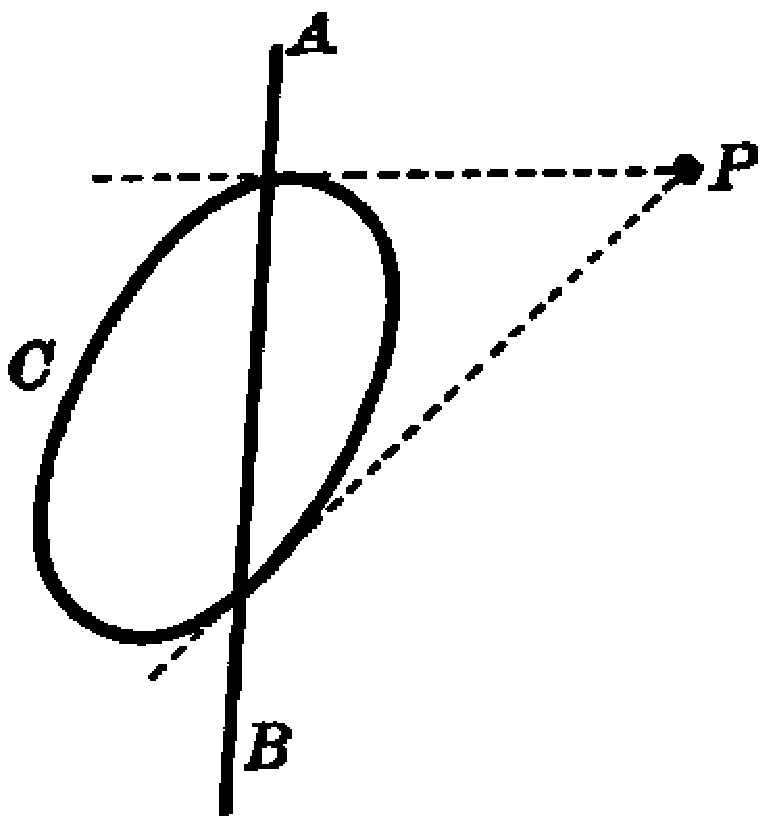
\includegraphics[scale=0.3]{images/Figure4.pdf}
\end{center}

We now restrict the discussion in the
remainder of this chapter to binary
forms.

We note that \emph{if the variables $(y)$ be replaced by the
variables $(x)$ in any polar of a form $f$ the result is $f$
itself}, \emph{i.e.} the original polarized form. This follows by
Euler's theorem on homogeneous \index{Euler's theorem} functions,
since

\[
{\left(y \frac{\partial}{\partial x}\right) f} ]_{y=x} = \left(x_1
\frac{\partial}{\partial x_1} + x_2 \frac{\partial}{\partial
x_2}\right) f = mf. \tag{62}
\]

In connection with the theorem on the transformed form
of Chapter I, Section 2, we may observe that \emph{the coefficients
of the transformed form are given by the polar formulas}
\begin{equation}
a'_0 = f(\lambda_1, \lambda_2) = f_0.\\
a'_1 = f_{0\mu}, a'_2 = f_{0\mu^2}, ..., a^{\prime}_m =
f_{0\mu^{m}}. \tag{63}
\end{equation}
The $r$th $y$-polar of $f$ is a \emph{doubly binary} form in the sets
$(y_1, y_2), (x_1, x_2)$ of degree-order $(r, m-r)$. We may however
\emph{polarize a number of times as to $(y)$ and then a number
of times as to another cogredient set $(z)$};
\begin{equation}
\left.{f_{y^r}}\right]_{z^2} = {\frac{(m-r)!(m-r-s)!} {m!(m-r)!} }
\left( y\frac{\partial}{\partial x} \right)^r \left(
z\frac{\partial}{\partial x} \right)^s f.\tag{64}
\end{equation}
This result is a function of three cogredient sets $(x), (y), (z)$.

Since the polar operator is a linear differential operator, it
is evident that the polar of a sum of a number of forms
equals the sum of the polars of these forms,
\[
(f + \phi + \cdots)_{y^r} = f_{y^r} + \phi_{y^r} + \cdots .
\]

\subsection{The polar of a product.}
We now develop a very important
formula giving the polar of the product of two
binary forms in terms of polars of the two forms.

If $F(x_1, x_2)$ is any binary form in $x_1, x_2$ of order $M$ and $(y)$
is cogredient to $(x)$, we have by Taylor's theorem, $k$ being
any parameter,

\begin{align*}
&F(x_1 + ky_1, x_2 + ky_2)\\
&= F(x_1, x_2) + k \left( y \frac{\partial}{\partial x} \right) F + k^2 \left( y \frac{\partial}{\partial x} \right)^2 \frac{F}{2!} + \cdots + k^r\left( y \frac{\partial}{\partial x} \right)^r \frac{F}{r!} + \cdots\\
&= F + \binom{M}{1}F_yk + \binom{M}{2}F_{y^2}k^2 + \cdots + \binom{M}{r}F_{y^r}k^r + \cdots. \tag{65}
\end{align*}
Let $F=f(x_l, x_2)\phi(x_l, x_2)$, the product of two binary forms
of respective orders $m$, $n$. Then the $r$th polar of this product
will be the coefficient of $k^r$ in the expansion of
\[
f(x_1 + ky_1, x_2 + ky_2) \times \phi(x_1 + ky_1, x_2 + ky_2),
\]
divided by $\binom{m+n}{r}$, by (65). But this expansion equals
\begin{align*}
\bigg[ f + \binom{m}{1}f_yk & +\binom{m}{2}f_{y^2}k^{2} + \ldots + \binom{m}{r} f_{y^r}k^r
+ \ldots \bigg] \bigg[ \phi + \binom{n}{1} \phi_{y}k \\
& + \binom {n}{2}\phi_{y^2}k^2 + \ldots + \binom {n}{r} \phi_{y^r}k^r + \ldots \bigg].
\end{align*}
Hence by direct multiplication,
\[
f\phi \bigg]_{y^{r}} = \frac{1}{\binom{m+n}{r}} \left[ \binom{m}{0} \binom{n}{r}
f\phi_{y^{r}} +
\binom{m}{1} \binom{n}{r-1}f_{y}\phi_{y^{r-1}} + \ldots + \binom{m}{r}
\binom{n}{0}f_{y^{r}}\phi
\right],
\]
or
\[
f \phi \bigg]_{y^{r}} = \frac{1}{\binom{m+n}{r}} \sum_{s=0}^{r} \binom{m}{s} \binom{n}{r-s}
f_{y^{s}}\phi_{y^{r-s}} \tag{66}
\]
This is the required formula.

The sum of the coefficients in the polar of a product is
unity. This follows from the fact (cf. (62)) that if ($y$)
goes into ($x$) in the polar of a product it becomes the original
polarized form.

An illustration of formula (66) is the following:

Let $f = a_0x_1^4 + \ldots$, $\phi = b_0x_1^2 + \ldots$. Then
\begin{align*}
f\phi \bigg]_{y^3} & = \frac{1}{20} \left[ \binom{4}{3} \binom{2}{0}f_{y^{3}}\phi +
\binom{4}{2}
\binom{2}{1} f_{y^{2}}\phi_y + \binom{4}{1} \binom{2}{2}f_y \phi_{y^{2}} \right] \\
 & = \frac{1}{5}f_{y^{3}}\phi + \frac{3}{5}f_{y^{2}}\phi_y + \frac{1}{5}f_y\phi_{y^{3}}.
\end{align*}


\subsection{Aronhold's polars.} \index{Aronhold's polar
operators}\index{Operators!Aronhold} The coefficients of the
transformed binary form are given by
\[
a'_r = f_{\mu^{r}} \left( \lambda_1, \lambda_2 \right) \left( r=0, \ldots, m\right).
\]
These are the linear transformations of the induced group (Chap.
I, \S 2). Let $\phi$ be a second binary form of the same order as
$f$,
\[
\phi=b_0x_1^m + mb_1x_1^{m-1}x_2+\ldots.
\]

Let $\phi$ be transformed by $T$ into $\phi'$. Then
\begin{equation*}
b'_r = \phi_{u^r}(\lambda_1, \lambda_2).
\end{equation*}
Hence the set $b_0$, $b_1$, $\cdots$, $b_m$ is cogredient to the
set $a_0$, $a_1$, $\cdots$, $a_m$,
under the induced group. It follows immediately by the
theory of Paragraph I that
\begin{align*}
\left(b' \frac{\partial}{\partial a'}\right) &\equiv b'_o \frac {\partial}{\partial a'_0} + \cdots + b'_m \frac {\partial}{\partial a'_m}\\
&= b_0\frac{\partial}{\partial a_0} + \cdots +
b_m\frac{\partial}{\partial a_m} \equiv
\left(b\frac{\partial}{\partial a}\right). \tag{67}
\end{align*}
That is, $\left(b\frac{\partial}{\partial a}\right)$ is an
invariant operation. It is called the Aronhold operator but was
first discovered by Boole in 1841. Operated upon any concomitant
of $f$ it gives a simultaneous concomitant of $f$ and $\phi$. If
$m = 2$, let
\begin{equation*}
I = a_0a_2 - a_1^2.
\end{equation*}
Then
\begin{equation*}
\left(b\frac{\partial}{\partial a}\right) I =
\left(b_0\frac{\partial}{\partial a_0} + b_1
\frac{\partial}{\partial a_1} + b_2\frac{\partial}{\partial
a_2}\right) I = a_0b_2 - 2a_1b_1 + a_2b_0.
\end{equation*}
This is $h$ (Chap. I, \S 1). Also
\begin{equation*}
2{\left(b\frac{\partial}{\partial a}\right)}^2 I = 4(b_0b_2 -
b_1^2),
\end{equation*}
the discriminant of $\phi$. In general, if $\psi$ is any concomitant
of $f$,
\begin{equation*}
\psi' = {(a'_0, \cdots, a'_m)}^i{(x'_1,x'_2)}^\omega =
(\lambda\mu)^\kappa(a_0, \cdots, a_m)^i(x_1,x_2)^\omega,
\end{equation*}
then
\begin{equation}
{\left(b'\frac{\partial}{\partial a'}\right)}^r \psi' =
{(\lambda\mu)}^\kappa {\left(b\frac{\partial}{\partial
a}\right)}^r \psi (r=0,1, \cdots, i)  \tag{68}
\end{equation}
are concomitants of $f$ and $\phi$. When $r = i$, the concomitant is
\begin{equation*}
x={(b_0, \cdots, b_m)}^i{(x_1,x_2)}^\omega.
\end{equation*}
The other concomitants of the series, which we call a series of
Aronhold's polars of $\psi$, are said to be
\emph{intermediate}\index{Intermediate concomitants} to $\psi$ and
$\chi$, and of the same \emph{type} as $\psi$. The theory of
\emph{types} will be referred to in the sequel.\index{Types}

\emph{All concomitants of a series of Aronhold's polars have the
same index $k$.}

Thus the following series has the index $k = 2$, as may be
verified by applying (52) of Section 3, Chapter II to each
form ($f = a_0 x_1^3 + \cdots; \phi = b_0 x_1^3 + \cdots$):

\begin{align*}
H &= (a_0 a_2 - a_1^2) x_1^2 + (a_0 a_3 - a_1 a_2) x_1 x_2 +
(a_1 a_3 - a_2^2) x_2^2, \\
\left(b \frac{\partial}{\partial a}\right) H &= (a_0 b_2 - 2 a_1
b_1 + a_2 b_0) x_1^2 +
(a_0 b_3 + a_3 b_0 - a_1 b_2 - a_2 b_1) x_1 x_2 \\
&\qquad + (a_1 b_3 - 2 a_2 b_2 + a_3 b_1) x_2^2, \\
\frac{1}{2}\left(b \frac{\partial}{\partial a}\right)^2 H &= (b_0
b_2 - b_1^2) x_1^2 + (b_0 b_3 - b_1 b_2) x_1 x_2 + (b_1 b_3 -
b_2^2) x_2^2.\end{align*}


\subsection{Modular polars.}
Under the group $T_p$, we have shown,
$x_1^p, x_2^p$ are cogredient to $x_1, x_2$. Hence the polar operation
\[
\delta_p = x_1^p \frac{\partial}{\partial x_1} + x_2^p
\frac{\partial}{\partial x_2}, \tag{69}
\]
applied to any algebraic form $f$, or covariant of $f$, gives a
formal modular concomitant of $f$. Thus if
\[
f = a_0 x_1^2 + 2 a_1 x_1 x_2 + a_2 x_2^2,
\]
then,
\[
\frac{1}{2} \delta_3 f = a_0 x_1^4 + a_1 (x_1^3 x_2 + x_1 x_2^3) + a_2 x_2^4.
\]
This is a covariant of $f$ modulo 3, \index{Arithmetical
invariants} as has been verified in Chapter I, Section 1. Under
the induced modular group $a_0^p, x_1^p, \cdots, a_m^p$ will be
cogredient to $a_0, a_1, \cdots, a_m$. Hence we have the modular
Aronhold operator
\[
d_p = a_0^p \frac{\partial}{\partial a_0} + \cdots + a_m^p
\frac{\partial}{\partial a_m}.
\]
If $m = 2$, and
\[
D = a_0 a_2 - a_1^2,
\]
then
\[
d_p D \equiv a_0^p a_2 - 2 a_1^{p+1} + a_0 a_2^p \pmod{p}.
\]
This is a formal modular invariant modulo $p$. It is not an
algebraic invariant; that is, not invariantive under the group
generated by the transformations $T$.

We may note in addition that the line
\[
l = a_0 x_1 + a_1 x_2 + a_2 x_3
\]
has among its covariants modulo 2, the line and the conic
\begin{align*}
     d_2 l &= a_0^2 x_1 + a_1^2 x_2 + a_2^2 x_3,\\
\delta_2 l &= a_0 x_1^2 + a_1 x_2^2 + a_2 x_3^2.
\end{align*}

\subsection{Operators derived from the fundamental postulate.}
The fundamental postulate on cogrediency (Chap. I, \S 2) enables
us to replace the variables in a concomitant by any set of
elements cogredient to the variables, without disturbing the
property of invariance.

\begin{Theorem}
Under the binary transformations $T$ the differential operators
$\frac{\partial}{\partial x_2},-\frac{\partial}{\partial x_1}$ are
cogredient to the variables.
\end{Theorem}

From $T$ we have
\begin{align*}
\frac{\partial}{\partial x'_1} &= \lambda_1 \frac{\partial}{\partial x_1} + \lambda_2 \frac{\partial}{\partial x_2},\\
\frac{\partial}{\partial x'_2} &= \mu_1 \frac{\partial}{\partial x_1} + \mu_2 \frac{\partial}{\partial x_2}.
\end{align*}
Hence
\begin{align*}
(\lambda \mu) \frac{\partial}{\partial x_2} &= \lambda_1 \frac{\partial}{\partial x'_2}
+ \mu_1 \left( -\frac{\partial}{\partial x'_1} \right),\\
-(\lambda \mu) \frac{\partial}{\partial x_1} &= \lambda_2 \frac{\partial}{\partial x'_2}
+ \mu_2 \left( -\frac{\partial}{\partial x'_1} \right).
\end{align*}
This proves the theorem.

It follows that if $\phi = (a_0, \hdots, a_m)^i (x_1,x_2)^\omega$ is any invariant
function, \emph{i.e}. a concomitant of a binary form $f$, then
\begin{equation}
\partial \phi = (a_0, \hdots, a_m)^i \left(\frac{\partial}{\partial x_2},-\frac{\partial}{\partial x_1} \right)^\omega
\tag{70}\end{equation} is an invariant operator (Boole). If this
operator is operated upon any covariant of $f$, it gives a
concomitant of $f$, and if operated upon a covariant of any set of
forms $g$, $h$, $\ldots$, it gives a simultaneous concomitant of
$f$ and the set. This process is a remarkably prolific one and
enables us to construct a great variety of invariants and
covariants of a form or a set of forms. We shall illustrate it by
means of several examples.

Let $f$ be the binary quartic and let $\phi$ be the form $f$ itself.
Then
$$
\partial \phi = \partial f = a_0\frac{\partial_4}{\partial x_2^4} - 4a_1\frac{\partial^4}{\partial x_2^3\partial x_1} + 6a_2\frac{\partial^4}{\partial x_2^2\partial x_1^2} - 4a_3\frac{\partial^4}{\partial x_2\partial x_1^3} + a_4\frac{\partial^4}{\partial x_1^4},
$$
and
$$
\frac{1}{24}\delta f \cdot f=2(a_0a_4 - 4a_1a_3 + 3a_2^2) = i.
$$
This second degree invariant $i$ represents the condition that
the four roots of the quartic form a self-apolar range. If
this process is applied in the case of a form of odd order, the
result vanishes identically.

If $H$ is the Hessian of the quartic, then
\begin{align*}
\partial H &= (a_0a_2 - a_1^2)\frac{\partial^4}{\partial x_2^4} - 2(a_0a_3 - a_1a_2)\frac{\partial^4}{\partial x_2^3\partial x_1}\\
&+(a_0a_4 + 2a_1a_3 - 3a_2^2)\frac{\partial^4}{\partial x_2^2\partial x_1^2} - 2(a_1a_4 - a_2a_3)\frac{\partial^4}{\partial x_2\partial x_1^3}\\
&+(a_2a_4 - a_3^2)\frac{\partial^4}{\partial x_1^4}.
\end{align*}
And
\begin{align*}
\frac{1}{12}\partial H\cdot f = 6(a_0a_2a_4 + 2a_1a_2a_3 - a_0a_3^2 - a_2^3) = J.  \tag{$70_1$}
\end{align*}
This third-degree invariant equated to zero gives the condition
that the roots of the quartic form a harmonic range.

If $H$ is the Hessian of the binary cubic $f$ and
$$
g = b_0x_1^3 + \ldots,
$$
then
\begin{align*}
\frac{1}{6}\partial H\cdot g &= [b_0(a_1a_3 - a_2^2) + b_1(a_1a_2 - a_0a_3) + b_2(a_0a_2 - a_1^2)]x_1\\
&+ [b_1(a_1a_3 - a_2^2) + b_2(a_1a_2 - a_0a_3) + b_3(a_0a_2 - a_1^2)]x_2;
\end{align*}
a linear covariant of the two cubics.

\subsubsection*{Bilinear Invariants}\index{Bilinear invariants}
If $f=a_0x_1^m + \cdots$ is a binary form of order $m$ and
$g=b_0x_1^m + \cdots$ another of the same order, then
\begin{equation}
\frac{1}{m!} \partial f \cdot g = a_0b_m - \binom{m}{1} a_1b_{m-1}
+
\cdots + (-1)^r\binom{m}{r} a_rb_{m-r}\\
+ \cdots + (-1)^m a_mb_0. \tag{71}
\end{equation}
This, the \emph{bilinear invariant} of $f$ and $g$, is the
simplest joint invariant of the two forms. If it is equated to
zero, it gives the condition that the two forms be \emph{apolar}.
If $m = 2$, the apolarity condition is the same as the condition
that the two quadratics be harmonic conjugates (Chap. I, \S 1,
IV). \index{Apolarity}

\subsection{The fundamental operation called
transvection.}\index{Transvectants, binary:!Definition} The most
fundamental process of binary invariant theory is a differential
operation called transvection. In fact it will subsequently appear
that all invariants and covariants of a form or a set of forms can
be derived by this process. We proceed to explain the nature of
the process. We first prove that the following operator $\Omega$
is an invariant:
\begin{equation}
\Omega = \begin{vmatrix}
\frac{\partial}{\partial x_1}, & \frac{\partial}{\partial x_2}\\
\frac{\partial}{\partial y_1}, & \frac{\partial}{\partial y_2}
\end{vmatrix}
\tag{72}
\end{equation}
where ($y$) is cogredient to ($x$). In fact by (70),
\begin{equation*}
\Omega' = \begin{vmatrix} \lambda_1 \frac{\partial}{\partial x_1}
+ \lambda_2 \frac{\partial}{\partial x_2}, &
\mu_1 \frac{\partial}{\partial x_1} + \mu_2 \frac{\partial}{\partial x_2}\\
\lambda_1 \frac{\partial}{\partial y_1} +
\lambda_2 \frac{\partial}{\partial y_2}, &
\mu_1 \frac{\partial}{\partial y_1} + \mu_2 \frac{\partial}{\partial y_2}
\end{vmatrix} = (\lambda \mu) \Omega,
\end{equation*}
which proves the statement.

Evidently, to produce any result, $\Omega$ must be applied to
a doubly binary function. One such type of function is a
$y$-polar of a binary form. But

\begin{Theorem}
The result of operating $\Omega$ upon any $y$-polar of
a binary form $f$ is zero.
\end{Theorem}

For, if $f = a_0x_1^m + \cdots$,
\begin{align*}
P &= \frac{m!}{(m-r)!}f_y^r = \left(y\frac{\partial}{\partial x}\right)^rf \\
&= \left(y_1^r\frac{\partial^r f}{\partial x_1^y} + \binom {r}{1}
y_1^{r-1}y_2 \frac{\partial^rf}{\partial x_1^{r-1}\partial x_2} +
\cdots + y_2^r\frac{\partial^r f}{\partial x_2^r}\right).
\end{align*}
Hence
\begin{align*}
\Omega P &= \binom{r}{1} y_1^{r-1}
\frac{\partial^{r+1}f}{\partial x_1^r\partial x_2} +
\cdots +
ry_2^{r-1}\frac{\partial^{r+1} f}{\partial x_1\partial x_2^r} \\
&- ry_1^{r-1}\frac{\partial^{r+1} f}{\partial x_1^r\partial x_2} -
\cdots - \binom{r}{1}y_2^{r-1}\frac{\partial^{r+1} f}{\partial x_1\partial x_2^r},
\end{align*}
and this vanishes by cancellation.

If $\Omega$ is operated upon another type of doubly binary form,
not a polar, as for instance upon $fg$, where $f$ is a binary form
in $x_1, x_2$ and $g$ a binary form in $y_1, y_2$, the result will generally
be a doubly binary invariant formation, not zero.

\subsubsection*{DEFINITION.}
If $f(x) = a_0x_1^m + \cdots$ is a binary form in ($x$)
of order $m$, and $g(y) = b_0y_1^n + \cdots$ a binary form in ($y$) of order
$n$, then if $y_1, y_2$ be changed to $x_1, x_2$ respectively in
\begin{align*}
\frac{(m-r)!(n-r)!}{m!n!} \Omega^rf(x)g(y), \tag{73}
\end{align*}
after the differentiations have been performed, the result is
called the $r$th transvectant (Cayley, 1846) of $f(x)$ and $g(x)$.
This will be abbreviated $(f, g)^r$, following a well-established
notation. We evidently have for a general formula
\begin{align*}
(f,g)^r = \frac{(m-r)!(n-r)!}{m!n!} \sum_{s=0}^r(-1)^s
\binom{r}{\delta} \frac{\partial^rf(x)}{\partial x_1^{r-s}\partial
x_2^s} \cdot \frac{\partial^rg(x)}{\partial x_1^s \partial
x_2^{r-s}}. \tag{74}
\end{align*}

We give at present only a few illustrations. We note that
the Jacobian of two binary forms is their first transvectant.
Also the Hessian of a form $f$ is its second transvectant. For
\begin{align*}
H &= \frac{2}{m^2 (m-1)^2} (f_{x_1 x_1} f_{x_2 x_2} - f^2_{x_1 x_2}) \\
&= \frac{(\lfloor\underline{m-2})^2}{(\lfloor\underline{m})^2} (f_{x_1 x_1}f_{x_2 x_2} - 2 f^2_{x_1 x_1} + f_{x_2 x_2}f_{x_1 x_1}) \\
&= (f, f)^2.
\end{align*}

As an example of multiple transvection we may write the
following covariant of the cubic $f$:

\begin{align*}
Q &= (f, (f, f)^2)^1 = (a_0^2 a_3 - 3 a_0 a_1 a_2 + 2 a_1^3)x^3 \\
&+ 3(a_0 a_1 a_3 - 2 a_0 a_2^2 + a_1^2 a_2)x_1^2 x_2 \\
&- 3(a_0 a_2 a_3 - 2 a_1^2 a_3 + a_1 a_2^2)x_1 x_2^2 \\
&- (a_0 a_3^2 - 3 a_1 a_2 a_3 + 2 a_2^3)x_2^3 \tag{$74_1$}
\end{align*}
If $f$ and $g$ are two forms of the same order $m$, then $(f, g)^m$ is
their bilinear invariant. By forming multiple transvections,
as was done to obtain $Q$, we can evidently obtain an unlimited
number of concomitants of a single form or of a set.

\section{The Aronhold Symbolism. Symbolical Invariant Processes}

\subsection{Symbolical Representation.}\index{Symbolical
theory:!binary} A binary form $f$, written in the notation of
which

\[
f = a_0 x_1^3 + 3 a_1 x_1^2 x_2 + 3 a_2 x_1 x_2^2 + a_3 x_2^3
\]
is a particular case, bears a close formal resemblance to a
power of linear form, here the third power. This resemblance
becomes the more noteworthy when we observe that
the derivative $\frac{\partial f}{\partial x_1}$ bears the same formal resemblance to the
derivative of the third power of a linear form:

\[
\frac{\partial f}{\partial x_1} = 3(a_0 x_1^2 + 2 a_1 x_1 x_2 + a_2 x_2^2) .
\]
That is, it resembles three times the square of the linear
form. When we study the question of how far this formal
resemblance may be extended we are led to a completely
new and strikingly concise formulation of the fundamental
processes of binary invariant theory. Although $f = a_0x^m + \cdots$
is not an exact power, we assume the privilege of placing it
equal to the $m$th power of a purely symbolical linear form
$\alpha_1x_1 + \alpha_2x_2$ which we abbreviate $\alpha_x$.
$$
f= (\alpha_1x_1+\alpha_2x_2)^m = \alpha_x^m = a_0x^m + \cdots.
$$
This may be done provided we assume that the only defined
combinations of the symbols $\alpha_1$, $\alpha_2$, that is, the only combinations
which have any definite meaning, are the monomials
of degree $m$ in $\alpha_1$, $\alpha_2$;
$$
\alpha_1^m = a_0, \alpha_1^{m-1}\alpha_2 = a_0, \cdots, \alpha_2^m = a_m,
$$
and linear combinations of these. Thus $\alpha_1^m+2\alpha_1^{m-1}\alpha_2^2$ means
$a_0+2a_2$.  But of $\alpha_1^{m-2}\alpha_2$ is meaningless; an umbral expression
(Sylvester). An expression of the second degree like $a_0a_8$
cannot then be represented in terms of $\alpha$'s alone, since
$\alpha_1^m \cdot \alpha_1^{m-3}\alpha_2^3 = \alpha_1^{2m-3}\alpha_2^3$ is undefined. To avoid this difficulty we
give $f$ a series of symbolical representations,
$$
f=\alpha_x^m = \beta_x^m = \gamma_x^m \cdots,
$$
wherein the symbols ($\alpha_1$, $\alpha_2$), ($\beta_1$, $\beta_2$), ($\gamma_1$, $\gamma_2$), ... are said to
be equivalent symbols as appertaining to the same form $f$.
Then
$$
\alpha_1^m =\beta_1^m = \gamma_1^m \cdots = a_0,
\alpha_1^{m-1} \alpha_2=\beta_1^{m-1} \beta_2= \gamma_1^{m-1}\gamma_2 \cdots = a_1, \cdots.
$$
Now $a_0a_3$ becomes ($\alpha_1^m\beta_1^{m-3}\beta_2^3$) and this is a defined combination
of symbols.

In general an expression of degree $i$ in the $a$'s will be represented
by means of $i$ equivalent symbol sets, the symbols of
each set entering the symbolical expressions only to the $m$th
degree; moreover there will be a series of (equivalent)
symbolical representations of the same expression, as
$$
a_0a_3 = \alpha_1^m\beta_1^{m-3}\beta_2^3 = \alpha_1^m\gamma_1^{m-3}\gamma_2^3=
\beta_1^m\gamma_1^{m-3}\gamma_2^3 = \cdots.
$$
Thus the discriminant of
\[
f=\alpha^2_x = \beta^2_x = \hdots = a_0x^2_1 + 2 a_1x_1x_2 + a_2x^2_2
\]
is
\begin{align*}
D & = 4(\alpha_0a_2 -a^2_1) = 4(\alpha^2_1\beta^2_2 - \alpha_1\alpha_2\beta_1\beta_2) \\
& = 2 (\alpha^2_1\beta^2_2 - 2\alpha_1\alpha_2\beta_1\beta_2 + \alpha^2_2 \beta^2_1),
\end{align*}
or
\[
D=2(\alpha\beta)^2,
\]
a very concise representation of this invariant.

Conversely, if we wish to know what invariant a given
symbolical expression represents, we proceed thus. Let $f$ be
the quadratic above, and
\[
g = \rho^2_x = \sigma^2_x = \hdots = b_0x^2_1 + 2b_1x_1x_2 + b_2x^3_2,
\]
where $\rho$ is not equivalent to $\alpha$. Then to find what
$J=(\alpha \rho)\alpha_x\rho_x$, which evidently contains the symbols in defined
combinations only, represents in terms of the actual
coefficients of the forms, we multiply out and find
\begin{align*}
J & = (\alpha_1\rho_2 - \alpha_2\rho_1)(\alpha_1x_1 + \alpha_2x_2) (\rho_1x_1 + \rho_2x_2) \\
& = (\alpha^2_1\rho_1\rho_2 - \alpha_1\alpha_2\rho^2_1)x^2_1 + (\alpha^2_1\rho^2_2 - \alpha^2_2\rho^2_1)x_1x_2 + (\alpha_1\alpha_2\rho^2_2 - \alpha^2_2\rho_1\rho_2)x^2_2, \\
& = (a_0b_1 - a_1b_0)x^2_1 + (a_0b_2 - a_2b_0)x_1x_2 + 9a_1b_2 -a_2b_1)x^2_2.
\end{align*}
This is the Jacobian of $f$ and $g$. Note the simple symbolical
form
\[
J=(\alpha\rho)\alpha_x\rho_x.
\]

\subsection{Symbolical polars.}\index{Determinant, symbolical}
We shall now investigate the forms
which the standard invariant processes take when expressed
in terms of the above symbolism (Aronhold, 1858).

For polars we have, when $f=\alpha^m_x = \beta^m_x = \hdots$,
\[
f_y = \frac{1}{m}\left( y\frac{\partial}{\partial x}\right) f = \alpha^{m-1}_x \left( y\frac{\partial}{\partial x}\right) (\alpha_1x_1 + \alpha_2x_2) = \alpha^{m-1}_x \alpha_y.
\]
Hence
\[
f_{y^r}=\alpha^{m-r}_x\alpha^r_y.
\tag{75}
\]

The {\it transformed form} of $f$ under $T$ will be
\begin{align*}
f' & = [\alpha_1(\lambda_1x'_1 + \mu_1x'_2) + \alpha_2(\lambda_2x'_1 + \mu_2x'_2)]^m \\
& = [(\alpha_1\lambda_1 + \alpha_2\lambda_2)x'_1 + \alpha_1 \mu_1 + \alpha_2\mu_2)x'_2]^m,
\end{align*}
or
\begin{align*} f^\prime &= (a_\lambda x^\prime_1 + a_\mu x^\prime_2)^m\\
&= a_\lambda^m x_1^{\prime m} + \hdots
+ \binom{m}{r} a_\lambda^{m-r} a_\mu^r x_1^{\prime m-r} x_2^{\prime r}
+ \hdots + a_\mu^m x_2^{\prime m}.
\tag{76}\end{align*}

In view of (75) we have here not only the symbolical
representation of the transformed form but a very concise
proof of the fact, proved elsewhere (Chap. I, (29)), that the
transformed coefficients are polars of
$a^\prime_0 = f(\lambda_1, \lambda_2) = a_\lambda^m$.

The formula (66) for the polar of a product becomes
\begin{equation}
\alpha_x^m \beta_x^n \Bigr]_{y^r}=
\frac{1}{\binom{m+n}{r}} \sum_{s=0}^r \binom{m}{s} \binom{n}{r-s}
\alpha_x^{m-s} \alpha_y^s \beta_x^{n-r+s} \beta_y^{r-s},
\tag{77}\end{equation}
where the symbols $\alpha$, $\beta$ are not as a rule equivalent.

\subsection{Symbolical transvectants.}
If $f = \alpha_x^m = a_x^m = \hdots, g = \beta_x^n = b_x^n = \hdots$, then
\begin{align*}
(f,g)^1 &= \frac{1}{mn} \Omega \alpha_x^m \beta_y^n \Bigr]_{y=x}
= \alpha_x^{m-1} \beta_y^{n-1}
\left( \frac{\partial^2}{\partial x_1 \partial y_2}
- \frac{\partial^2}{\partial x_2 \partial y_1}\right) \alpha_x \beta_y
\Bigr]_{y=x}\\
&=(\alpha \beta) \alpha_x^{m-1} \beta_x^{n-1}.
\end{align*}
Hence the symbolical form for the $r$th transvectant is
\begin{equation}
(f,g)^r = (\alpha \beta)^r \alpha_x^{m-r} \beta_x^{n-r}.
\tag{78}\end{equation}
Several properties of transvectants follow easily from this.
Suppose that $g = f$ so that $\alpha$ and $\beta$ are equivalent symbols.
Then obviously we can interchange $\alpha$ and $\beta$ in any symbolical
expression without changing the value of that expression.
Also we should remember that $(\alpha \beta)$ is a determinant of the
second order, and \emph{formally}
\[
(\alpha \beta) = - (\beta \alpha).
\]
Suppose now that $r$ is odd, $r = 2 k + 1$. Then
\[
(f,f)^{2k+1} = (\alpha \beta)^{2k+1} a_x^{m-2k-1} \beta^{n-2k-1}
= - (\alpha \beta)^{2k+1} a_x^{m-2k-1} \beta_x^{n-2k-1}
\]
Hence this transvectant, being equal to its own negative,
vanishes. \emph{Every odd transvectant of a form with itself vanishes}.

If the symbols are not equivalent, evidently
\begin{equation}
(f,g)^r = (-1)^r (g,f)^r.
\tag{79}\end{equation}
Also if $C$ is a constant,
\begin{align*}
(Cf,g)^r &= C (f,g)^r; \tag{80}\\
(c_1 f_1 + c_2 f_2 + \hdots, d_1 g_1 + d_2 g_2 + \hdots)^r
&= c_1 d_1 (f_1,g_1)^r + c_1 d_2 (f_1,g_2)^r + \hdots. \tag{81}
\end{align*}

\subsection{Standard method of transvection.}\index{Standard
method of transvection:!binary}We may derive transvectants from
polars by a simple application of the fundamental postulate. For,
as shown in section 1, if $f = a_0 x_1^m + \hdots = a_x^m$,
\begin{equation}
f_{y^r} = \frac{(m-r)!}{m!} \left[\frac{\partial f}{\partial
x_1^r} y_1^r + \binom{r}{1} \frac{\partial^r f}{\partial x_1^{r-1}
\partial x_2} y_1^{r-1} y_2 + \hdots + \frac{\partial^r
f}{\partial x_2^r} y_2^r \right]. \tag{82}\end{equation} Now $(y)$
is cogredient to $(x)$. Hence $\frac{\partial}{\partial x_2},
-\frac{\partial}{\partial x_1}$ are cogredient to $y_1, y_2$. If
we replace the $y$'s by these derivative symbols and operate the
result, which we abbreviate as $\partial f_{y^r}$, upon a second
form $g = b_x^n$, we obtain
\begin{align*}
\frac{(n-r)!}{n!} \partial f_{y^r} \\
&=\left[a_1^r b_2^r - \binom{r}{1} a_1^{r-1} a_2 b_2^{r-1} b_1 +
\hdots + (-1)^r a_2^r b_1^r\right]
a_x^{m-r} b_x^{n-r}\\
&= (ab)^r a_x^{m-r} b_x^{n-r} = (f,g)^r.
\tag{83}\end{align*}
When we compare the square bracket in (82) with $a_x^{m-r}$
times the square bracket in (83), we see that they differ
precisely in that $y_1, y_2$ has been replaced by $b_2, -b_1$. Hence
we enunciate the following \emph{standard method of transvection}.
Let $f$ be any symbolical form. It may be simple like $f$ in
this paragraph, or more complicated like (78), or howsoever
complicated. To obtain the $r$th transvectant of $f$ and $\phi = b_x^n$
we \emph{polarize $f$ $r$ times, change $y_1, y_2$ into $b_2, -b_1$
respectively in
the result and multiply by $b_x^{n-r}$.} In view of the formula (77)
for the polar of a product this is the most desirable method
of finding transvectants.

For illustration, let $F$ be a quartic, $F = a_x^4 = b_x^4$, and $f$ its
Hessian,
\[
f = (ab)^2 a_x^2 b_x^2.
\]
Let
\[
g = \alpha_x^3.
\]
Then
\begin{align*}
(f,g)^2 &= (ab)^2 a_x^2 b_x^2 \Bigr]_{y^2,y=a} \times \alpha_x \\
&= \frac{(ab)^2}{6} \left[\binom{2}{0} \binom{2}{2} a_x^2 b_y^2
                         + \binom{2}{1} \binom{2}{1} a_x a_y b_x b_y
                         + \binom{2}{2} \binom{2}{0} a_y^2 b_x^2\right]_{y=a} \times \alpha_x \tag{84}\\
&= \frac{1}{6} (ab)^2 (b \alpha)^2 a_x^2 \alpha_x
   + \frac{2}{3} (ab)^2 (a \alpha) (b \alpha) a_x b_x \alpha_x
   + \frac{1}{6} (ab)^2 (a \alpha)^2 b_x^2 \alpha_x.
\end{align*}

Since the symbols $a, b$ are equivalent, this may be simplified
by interchanging $a, b$ in the last term, which is then identical
with the first,
\[
(f,g)^2 = \frac{1}{3} (ab)^2 (b \alpha)^2 a_x^2 \alpha_x
        + \frac{2}{3} (ab)^2 (a \alpha) (b \alpha) a_x b_x \alpha_x.
\]

By the fundamental existence theorem this is a joint covariant
of $F$ and $g$.

Let $f$ be as above and $g = (\alpha \beta) \alpha_x^2 \beta_x$, where $\alpha$ and $\beta$ are not
equivalent. To find $(f,g)^2$, say, in a case of this kind we
first let
\[
g = (\alpha \beta) \alpha_x^2 \beta_x = \sigma_x^3,
\]
introducing a new symbolism for the cubic $g$. Then we
apply the method just given, obtaining
\[
(f,g)^2 = \frac{1}{3} (ab)^2 (b \sigma)^2 a_x^2 \sigma_x
        + \frac{2}{3} (ab)^2 (a \sigma) (b \sigma) a_x b_x \sigma_x.
\]
We now examine this result term by term. We note that
the first term could have been obtained by polarizing $g$ twice
changing $y_1, y_2$ into $b_2, -b_1$ and multiplying the result by
$(ab)^2a_x^2$. Thus
\begin{equation}
\frac{1}{3} (ab)^2 (b \sigma)^2 a_x^2 \sigma_x =
\frac{1}{3}(\alpha \beta) \alpha_x^2 \beta_x \Bigr]_{y^2; y=b}
(ab)^2 a_x^2. \tag{85}\end{equation} Consider next the second
term. It could have been obtained by polarizing $g$ once with
regard to $y$, and then the result once with regard to $z$; then
changing $y_1, y_2$ into $a_2, -a_1$, and $z_1, z_2$ into $b_2,
-b_1$, and multiplying this result by $(ab)^2 a_x b_x$;
\begin{align*}
\frac{2}{3} (ab)^2 (a \sigma) (b \sigma) a_x b_x \sigma_x & \\ &=
\left. \left. \frac{2}{3} (\alpha \beta) \alpha_x^2 \beta_x
\right]_{y; y=a} \right]_{z; z=b} \times (ab)^2 a_x b_x. \tag{86}
\end{align*}
From (85),
\[
\frac{1}{9} (\alpha \beta) \left[ \binom{2}{1} \binom{1}{1} \alpha_x \alpha_y \beta_y + \binom{2}{2} \binom{1}{0} \alpha_y^2 \beta_x \right]_{y=b}(ab)^2 a_x^2
\]
\[
= \frac{2}{9} (ab)^2 (\alpha \beta) (ab) (\beta b) a_x^2 \alpha_x + \frac{1}{9} (ab)^2 (\alpha \beta) (ab)^2 a_x^2 \beta_x.
\]
From (86),
\begin{align*}
&\frac{2}{9} (\alpha \beta) \left. \left[ \binom{2}{0} \binom{1}{1} \alpha_x^2 \beta_y + \binom{2}{1} \binom {1}{0} \alpha_x \alpha_y \beta_x \right]_{y=a} \right]_{z; z=b} (ab)^2 a_x b_x \\
&= \left. \frac{2}{9} \alpha_x^2 (\beta a) + \frac{4}{9} \alpha_x \beta_x (\alpha a) \right]_{z; z=b}  \times (ab)^2 (\alpha \beta) a_x b_x
\end{align*}
\begin{align*}
= \frac{2}{9} (ab)^2 (\alpha \beta) (\alpha b) (\beta a) \alpha_x a_x b_x &+ \frac{2}{9} (ab)^2 (\alpha \beta) (\alpha a)(\alpha b) \beta_x a_x b_x \\
&+ \frac{2}{9} (ab)^2 (\alpha \beta) (\beta b) (\alpha a) \alpha_x a_x b_x.
\end{align*}
Hence we have in this case
\begin{align*}
(f,g)^2 = \frac{2}{9}(ab)^2 (\alpha \beta) (\alpha b)(\beta b) a_x^2 a_x + \frac{1}{9} (ab)^2 (\alpha \beta) (ab)^2 a_x^2 \beta_x \\
+ \frac{4}{9} (ab)^2 (\alpha \beta) (\alpha b) (\beta a) \alpha_x a_x b_x + \frac{2}{9} (ab)^2 (\alpha \beta) (\alpha a)(\alpha b) \beta_x a_x b_x. \tag{87}
\end{align*}

\subsection{Formula for the $r$th transvectant.}
The most general
formulas for $f, g$ respectively are

\[
f = \alpha_x^{(1)} \alpha_x^{(2)} \cdots \alpha_x^{(m)}, g  = \beta_y^{(1)} \beta_y^{(2)} \cdots \beta_y^{(n)},
\]
in which
\[
a_x^{(i)} = a_1^{(i)} x_1 + a_x^{(i)} x_2, \beta_x^{(i)} = \beta_1^{(i)} x_1 + \beta_2^{(i)} x_2.
\]
We can obtain a formula of complete generality for the
transvectant $(f, g)^r$ by applying the operator $\Omega$ directly to the product $fg$. We have

\begin{align*}
\frac{\partial ^2}{\partial x_1 \partial y_2} fg &= \sum \alpha_1^{(q)} \beta_2^{(r)} \frac{fg}{\alpha_x^{(q)} \beta_y^{(r)}}, \\
\frac{\partial^2}{\partial x_2 \partial y_1} fg &= \sum \alpha_2^{(q)} \beta_1^{(r)} \frac{fg}{\alpha_x^{(q)} \beta_y^{(r)}}.
\end{align*}
Subtracting these we obtain
\[
(f,g)^1=\frac{(m-1)!(n-1)!}{m!n!}
\sum(\alpha^{(q)}\beta^{(r)})\frac{fg}{\alpha_x^{(q)}\beta_x^{(r)}}.
\]
Repetitions of this process, made as follows:
\begin{equation}
(f,g)^2 = \frac{(m-2)!(n-2)!}{m!n!}
\sum(\alpha^{(q)}\beta^{(r)})\Omega\left[\frac{fg}{\alpha_x^{(q)}\beta_y^{(r)}}\right]_{y=x},
\tag{88}\end{equation} lead to the conclusion that the $r$th
transvectant of $f$ and $g$, as well as the mere result of
applying the operator $\Omega$ to $fg$ $r$ times, is a sum of
terms each one of which contains the product of $r$ determinant
factors $(\alpha\beta), m-r$ factors $\alpha_x$, and $n-r$ factors
$\beta_x$. We can however write $(f, g)^r$ in a very simple
explicit form. Consider the special case
\[
f=\alpha_x^{(1)}\alpha_x^{(2)}\alpha_x^{(3)},\  g=\beta_y^{(1)}\beta_y^{(2)}.
\]
Here, by the rule of (88),
\begin{align*}
(f,g)^2&=\{(\alpha^{(1)}\beta^{(1)})(\alpha^{(2)}\beta^{(2)})\alpha_x^{(3)} + (\alpha^{(1)}\beta^{(1)})(\alpha^{(3)}\beta^{(2)})\alpha_x^{(2)}\\
       &+ (\alpha^{(1)}\beta^{(2)})(\alpha^{(2)}\beta^{(1)})\alpha_x^{(3)} + (\alpha^{(1)}\beta^{(2)})(\alpha^{(3)}\beta^{(1)})\alpha_x^{(2)}\\
       &+ (\alpha^{(2)}\beta^{(1)})(\alpha^{(3)}\beta^{(2)})\alpha_x^{(1)} + (\alpha^{(2)}\beta^{(1)})(\alpha^{(1)}\beta^{(2)})\alpha_x^{(3)}\tag{89}\\
       &+ (\alpha^{(2)}\beta^{(2)})(\alpha^{(3)}\beta^{(1)})\alpha_x^{(1)} + (\alpha^{(2)}\beta^{(2)})(\alpha^{(1)}\beta^{(1)})\alpha_x^{(3)}\\
       &+ (\alpha^{(3)}\beta^{(1)})(\alpha^{(1)}\beta^{(2)})\alpha_x^{(2)} + (\alpha^{(3)}\beta^{(1)})(\alpha^{(2)}\beta^{(2)})\alpha_x^{(1)}\\
       &+ (\alpha^{(3)}\beta^{(2)})(\alpha^{(1)}\beta^{(1)})\alpha_x^{(2)} + (\alpha^{(3)}\beta^{(2)})(\alpha^{(2)}\beta^{(1)})\alpha_x^{(1)} \div 2!3!,
\end{align*}
{\loosen
in which occur only six distinct terms, there being a repetition
of each term. Now consider the general case, and the $r$th
transvectant. In the first transvectant one term contains $t_1 =
(\alpha^{(1)}\beta^{(1)})\alpha_x^{(2)}\cdots\alpha_x^{(m)}\beta_y^{(2)}\cdots\beta_y^{(n)}$.
In the second transvectant there will be a term $u_1=
(\alpha^{(1)}\beta^{(1)})(\alpha^{(2)}\beta^{(2)})\alpha_x^{(3)}\cdots\beta_y^{(3)}\cdots
$ arising from $\Omega t_1$, and another term $u_1$ arising from
$\Omega t_2$, where
$t_2=(\alpha^{(2)}\beta^{(2)})\alpha_x^{(1)}\alpha_x^{(3)} \cdots
\alpha_x^{(m)} \beta_y^{(1)} \beta_y^{(3)} \cdots \beta_y^{(n)}$.
Thus $u_1(y=x)$ and likewise any selected term occurs just twice
in $(f,g)^2$. Again the term $v_1 =
(\alpha^{(1)}\beta^{(1)})(\alpha^{(2)}\beta^{(2)})(\alpha^{(3)}\beta^{(3)})\alpha_x^{(4)}
\cdots \beta_x^{(4)} \cdots$ will occur in $(f, g)^3$ as many
times as there are ways of permuting the three superscripts $1, 2,
3$ or $3!$ times. Finally in $(f,g)^r$, written by (88) in the
form (89), each term will be repeated $r!$ times. We may therefore
write $(f, g)^r$ as the following summation, in which all terms
are distinct and equal in number to $\binom{m}{r} \binom{n}{r}
r!$:}
\begin{equation}
(f, \phi)^r = \frac{1}{\binom{m}{r} \binom{n}{r}r!}
              \sum \left[\frac{(\alpha^{(1)} \beta^{(1)}) (\alpha^{(2)} \beta^{(2)}) \hdots
                                (\alpha^{(r)} \beta^{(r)})}
                          {\alpha_x^{(1)} \alpha_x^{(2)} \hdots \alpha_x^{(m)}
                           \beta_y^{(1)} \beta_y^{(2)} \hdots \beta_y^{(n)}} fg \right]_{y=x}.
\tag{90}\end{equation}

\subsection{Special cases of operation by $\Omega$ upon a doubly binary
form, not a product.}
In a subsequent chapter Gordan's series
will be developed. This series has to do with operation by $\Omega$
upon a doubly binary form which is neither a polar nor a
simple product. In this paragraph we consider a few very
special cases of such a doubly binary form and in connection
therewith some results of very frequent application.

We can establish the following formula:
\begin{equation}
\Omega^r(xy)^r = constant = (r + 1)(r!)^2. \tag{91}\end{equation}
In proof (74),
\[
\Omega^r = \sum_{i=0}^r (-1)^i \binom{r}{i} \frac{\partial^r}{\partial x_1^{r-i} \partial x_2^i}
                                            \frac{\partial^r}{\partial y_1^i \partial y_2^{r-i}},
\]
and
\[
(xy)^r = \sum_{i=0}^r (-1)^i \binom{r}{i} x_1^{r-i} x_2^i y_1^i y_2^{r-i}.
\]
Hence it follows immediately that
\begin{align*}
\Omega^r (xy)^r &= \sum_{i=0}^r \binom{r}{i}^2 ((r-i)!)^2 (i!)^2 \\
                &= \sum_{i=0}^r (r!)^2 = (r+1) (r!)^2.
\end{align*}
A similar doubly binary form is
\[
F = (xy)^j \xi_x^{m-j} \xi_y^{n-j}.
\]
If the second factor of this is a polar of $\xi_x^{m+n-2j}$, we may
make use of the fact, proved before, that $\Omega$ on a polar is zero.
An easy differentiation gives
\[
\Omega F = j(m+n-j+1)(xy)^{j-1} \xi_x^{m-j} \xi_y^{n-j},
\]
and repetitions of this formula give
\begin{equation}
\Omega^i F = \frac{j!}{(j-1)!} \frac{(m+n-j+1)!}{(m+n-j-i+1)!}
(xy)^{j-i} \xi_x^{m-j} \xi_y^{n-j} \binom{\text{If } i\leqq j;}{=0
\text{ if } i > j} \tag{$91_1$}\end{equation}

This formula holds true if $m = n = j$, that is, for $\Omega^i (xy)^j$.

\subsection{Fundamental theorem of symbolical theory.}
\begin{Theorem}
Every monomial expression $\phi$ which consists
entirely of symbolical factors of two types, e.g. determinants
of type $(\alpha \beta)$ and linear factors of the type $\alpha_x$ and which is a defined
expression in terms of the coefficients and variables of a
set of forms $f, g, \hdots$ is a concomitant of those forms. Conversely,
every concomitant of the set is a linear combination of
such monomials.\end{Theorem}

Examples of this theorem are given in (78), (84), (87).

In proof of the first part, let
\[
\phi = (\alpha \beta)^p (\alpha \gamma)^q \hdots \alpha_x^\rho \beta_x^\sigma \gamma_x^\tau \hdots,
\]
where $f = \alpha_x^m$; and $\beta, \gamma, \hdots$ may or may not be equivalent to
$\alpha$, depending upon whether or not $\phi$ appertains to a single
form $f$ or to a set $f, g, \dots$. Transform the form $f$, that is, the
set, by $T$. The transformed of $f$ is (76)
\[
f' = (\alpha_\lambda x'_1 + \alpha_\mu x'_2)^m.
\]

Hence on account of the equations of transformation,
\[
\phi' = (\alpha_\lambda \beta_\mu - \alpha_\mu \beta_\lambda)^p
        (\alpha_\lambda \gamma_\mu - \alpha_\mu \gamma_\lambda)^q
        \hdots \alpha_x^\rho \beta_x^\sigma \hdots
\]
But
\begin{equation}
\alpha_\lambda \beta_\mu - \alpha_\mu \beta_\lambda = (\lambda \mu)(\alpha \beta).
\tag{92}\end{equation}
Hence
\[
\phi' = (\lambda \mu)^{p+q+\hdots}\phi,
\]
which proves the invariancy of $\phi$. Of course if all factors
of the second type, $\alpha_x$, are missing in $\phi$, the latter is an \emph{invariant}.

To prove the converse of the theorem let $\phi$ be a concomitant
of the set $f, g, \hdots$ and let the corresponding invariant
relation be written
\[ \phi(a_0',a_1',\dots;x_1',x_2')=(\lambda \mu)^k \phi(a_0,a_1,\dots;x_1,x_2).
\tag{93}\]
Now $a'_j = \alpha_\lambda^{m-j}\alpha_\mu^j (j = 0, 1,\dots m)$. Hence if we substitute
these symbolical forms of the transformed coefficients, the left-hand side of (93) becomes a summation of the type
\[ \sum PQ{x_1'}^{\omega_1}{x_2'}^{\omega_1}=(\lambda \mu)^k\phi(a_0,\dots;x_1,x_2) \quad
(\omega_1 + \omega_2 = \omega), \tag{94} \]
where $P$ is a monomial expression consisting of factors of the
type $\alpha_\lambda$ only and $Q$ a monomial whose factors are of the one type
$\alpha_{\mu}$. But the inverse of the transformation $T$ (cf. (10)) can be written
\[ x_1' = \frac{\xi_\mu}{(\lambda \mu)}, \quad x_2' = \frac{\xi_\lambda}{(\lambda \mu)},\]
where $\xi_1 = -x_2, \xi_2 = x_1$. Then (94) becomes
\[ \sum (-1)^{\omega_2}PQ\xi_\mu^{\omega_1}\xi_\lambda^{\omega_2}=(\lambda
\mu)^{k+\omega}\phi \tag{95} \]
We now operate on both sides of (95) by $\Omega^{k+\omega}$, where
\[ \Omega = \frac{\partial^2}{\partial \lambda_1\partial \mu_2} -
\frac{\partial^2}{\partial \lambda_2\partial \mu_1}.\]
We apply (90) to the left-hand side of the result and (91) to the right-hand side. The
left-hand side accordingly becomes a sum of terms each term of which involves necessarily
$\omega + k$ determinants $(\alpha\beta)$, $(\alpha \xi)$. In fact, since the result is
evidently still of order $\omega$ in $x_1$, $x_2$ there will be in
each term precisely $\omega$ determinant factors of type $(\alpha \xi)$ and $k$ of type
$(\alpha \beta)$. There will be no factors of type $\alpha_\lambda$ or $\xi_\lambda$
remaining on the left since by (91) the right-hand side becomes a constant times $\phi$,
and $\phi$ does not involve $\lambda,\mu$. We now replace, on the left, $(\alpha \xi)$ by
its equivalent $\alpha_x$, $(\beta \xi)$ by $\beta_x$, etc.
Then (95) gives, after division by the constant on the right,
\[ \phi = \Sigma a(\alpha \beta)^p(\alpha \gamma)^q\dots \alpha_x^p \beta_x^\sigma \dots,
\tag{96}\]
where $a$ is a constant; which was to be proved.

This theorem is sometimes called the fundamental theorem
of the symbolical theory since by it any binary invariant
problem may be studied under the Aronhold symbolical
representation.

\section{Reducibility. Elementary Complete Irreducible
Systems}\index{Reduction}

Illustrations of the fundamental theorem proved at the
end of Section 2 will now be given.

\subsection{Illustrations.}
It will be recalled that in (96) each symbolical
letter occurs to the precise degree equal to the \emph{order
of the form} to which it appertains. Note also that $k + \omega$, the
index plus the order of the concomitant, used in the proof of
the theorem, equals the \emph{weight} of the concomitant. This
equals the number of symbolical determinant factors of the
type $(\alpha \beta)$ plus the number of linear factors of the type $\alpha_x$ in
any term of $\phi$. The \emph{order $\omega$ of the concomitant} equals the
number of symbolical factors of the type $\alpha_x$ in any term of $\phi$.
The \emph{degree} of the concomitant equals the number of distinct
symbols $\alpha, \beta, \hdots$ occurring in its symbolical representation.

Let
\[
\phi = (\alpha \beta)^p (\alpha \gamma)^q (\beta \gamma)^r \hdots \alpha_x^\rho \beta_x^\sigma \hdots
\]
be any concomitant formula for a set of forms $f = \alpha_x^m, g = \beta_x^n, \hdots$.
No generality will be lost in the present discussion
by assuming $\phi$ to be monomial, since each separate
term of a sum of such monomials is a concomitant. In order
to write down all \emph{monomial concomitants of the set of a given
degree} $i$ we have only to construct all symbolical products $\phi$
involving precisely $i$ symbols which fulfill the laws
\begin{align*}
p + q + &\hdots + \rho = m, \\
p + r + &\hdots + \sigma = n, \tag{97}\\
\hdots \hdots &\hdots \hdots \hdots
\end{align*}
where, as stated above, $m$ is the order of $f$ and equal therefore
to the degree to which $\alpha$ occurs in $\phi$, $n$, the order of $g$,
and so on.

In particular let the set consist of $f = \alpha^2_x = \beta^2_x$ merely.
For the concomitant of degree 1 only one symbol may be
used. Hence $f = \alpha^2_x$ itself is the only concomitant of degree
1. If $i = 2$, we have for $\phi$,
\[
\phi = (\alpha\beta)^p \alpha^\rho_x\beta^\sigma_x,
\]
and from (97)
\[
p + \rho = p + \sigma = 2.
\]
Or
\begin{center}
\begin{tabular}{|c|c|c|}
$p$ & $\rho$ & $\sigma$ \\
\hline
0 & 2 & 2 \\
1 & 1 & 1 \\
2 & 0 & 0
\end{tabular}
\end{center}
Thus the only monomial concomitants of degree 2 are
\[
\alpha^2_x\beta^2_x = f^2, (\alpha\beta)\alpha_x\beta_x \equiv
-(\alpha\beta)\alpha_x\beta_x \equiv 0, (\alpha\beta)^2 = \frac{1}{2} D.
\]
For the degree 3
\begin{align*}
\phi & = (\alpha\beta)^p(\alpha\gamma)^q(\beta\gamma)^r\alpha^\rho_x\beta^\sigma_x\gamma^\tau_x,\\
p + q + \rho & = 2, p + r + \sigma = 2, q + r + \tau = 2.
\end{align*}
It is found that all solutions of these three linear Diophantine
equations lead to concomitants expressible in the form
$f^sD^t$, or to identically vanishing concomitants.

\subsubsection*{DEFINITION.}
Any concomitant of a set of forms which is
expressible as a rational integral function of other concomitants
of equal or of lower degree of the set is said to be
\emph{reducible} in terms of the other concomitants.

It will be seen from the above that the only irreducible
concomitants of a binary quadratic \index{Quadratic} $f$ of the
first three degrees are $f$ itself and $D$, its discriminant. It
will be proved later that $f$, $D$ form a \emph{complete
irreducible system} of $f$. By this we mean a system of
concomitants such that every other concomitant of $f$ is reducible
in terms of the members of this system. Note that this system for
the quadratic is finite. In another chapter we shall prove the
celebrated \emph{Gordan's theorem} that a complete irreducible
system of concomitants exists for every binary form or set of
forms and the system consists always of a finite number of
concomitants.\index{Finiteness:! algebraical concomitants} All of
the concomitants of the quadratic $f$ above which are not monomial
are reducible, but this is not always the case as it will be
sometimes preferable to select as a member of a complete
irreducible system a concomitant which is not monomial (cf. (87)).
As a further illustration let the set of forms be $f = \alpha_x^2
= \beta_x^2 = \hdots, g = a_x^2 = b_x^2 = \hdots$; let $i = 2$.
Then employing only two symbols and avoiding $(\alpha \beta)^2 =
\frac{1}{2} D$, etc.
\begin{align*}
\phi &= (\alpha a)^p \alpha_x^\rho a_x^\sigma, \\
p + \rho &= p + \sigma = 2.
\end{align*}
The concomitants from this formula are,
\[
\alpha_x^2 a_x^2 = f \cdot g, (\alpha a) \alpha_x a_x = J, (\alpha a)^2 = h,
\]
$J$ being the Jacobian, and $h$ the bilinear invariant of $f$ and $\phi$.

\subsection{Reduction by identities.}
As will appear subsequently
the standard method of obtaining complete irreducible systems
is by transvection. There are many methods of proving
concomitants reducible more powerful than the one
briefly considered above, and the interchange of equivalent
symbols. One method is reduction by symbolical identities.

\emph{Fundamental identity}. \index{Identities,
fundamental:!binary}One of the identities frequently employed in
reduction is one already frequently used in various connections,
viz. formula (92). We write this
\begin{equation}
a_x b_y - a_y b_x \equiv (ab)(xy).
\tag{98}\end{equation}

\emph{Every reduction formula to be introduced in this book, including
Gordan's series and Stroh's series, may be derived
directly from} (98). For this reason this formula is called
the fundamental reduction formula of binary invariant theory
(cf. Chap. IV).

If we change $y_1$ to $c_2$, $y_2$ to $-c_1$, (98) becomes
\[
(bc) a_x + (ca) b_x + (ab) c_x \equiv 0.
\tag{99}
\]
Replacing $x$ by $d$ in (99),
\[
(ad)(bc) + (ca)(bd) + (ab)(cd) \equiv 0.
\tag{100}
\]
From (99) by squaring,
\[
2(ab)(ac)b_x c_x \equiv (ab)^2 c_x^2 + (ac)^2 b_x^2 - (bc)^2 a_x^2.
\tag{101}\]
If $\omega$ is an imaginary cube root of unity, and
\[
u_1 = (bc) a_x, u_2 = (ca) b_x, u_3 = (ab) c_x,
\]
we have
\begin{align*}
& (u_1 + u_2 + u_3) (u_1 + \omega u_2 + \omega^2 u_3) (u_1 + \omega^2 u_2 + \omega u_3)\\
& = (ab)^3 c_x^3 + (bc)^3 a_x^3 + (ca)^3 b_x^3 - 3(ab)(bc)(ca)a_x b_x c_x \equiv 0.
\tag{102}
\end{align*}
Other identities may be similarly obtained.

In order to show how such identities may be used in performing
reductions, let $f = a_x^3 = b_x^3 = \cdots$ be the binary cubic
form. Then
\begin{align*}
\Delta & = (f, f)^2 = (ab)^2 a_x b_x,\\
Q & = (f, \Delta) = (ab)^2 (cb) a_x c_x^2.
\end{align*}
\begin{align*}
-(f,Q)^2  & = \frac{1}{3} (ab)^2 (bc) [a_x c_y^2 + 2 c_x c_y a_y]_{y = d} \times d_x
\tag{$102_1$} \\
& = \frac{1}{3} [(ab)^2 (cd)^2 (bc) a_x d_x + 2 (ab)^2 (ad)(cd)(bc) c_x d_x].
\end{align*}
But by the interchanges $a \sim d, b \sim c$
\[
(ab)^2 (cd)^2 (bc) a_x d_x = (dc)^2 (ba)^2 (cb) a_x d_x \equiv 0.
\]
By the interchange $c \sim d$ the second term in the square
bracket equals
\[
(ab)^2 (cd) c_x d_x [(ad)(bc) + (ca)(bd)],
\]
or, by (100) this equals
\[
(ab)^3 (cd)^2 c_x d_x \equiv 0.
\]
Hence $(f,Q)^2$ vanishes.

We may note here the result of the transvection $(\Delta,\Delta)^2$;
\[
R = (\Delta,\Delta)^2 = (ab)^2 (cd)^2 (ac) (bd).
\]

\subsection{Concomitants of binary cubic.}
We give below a table of transvectants for the binary cubic form.
It shows which transvectants are reducible in terms of other
concomitants. It will be inferred from the table that the complete
irreducible system for the binary cubic $f$ consists of
\index{Cubic, binary:!fundamental system}
\[
f, \Delta, Q, R,
\]
one invariant and three covariants, and this is the case as
will be proved later. Not all of the reductions indicated in
this table can be advantageously made by the methods introduced
up to the present, but many of them can. All four
of the irreducible concomitants have previously been derived
in this book, in terms of the actual coefficients, but they are
given here for convenient reference:
\begin{align*}
f =& a_0x_1^3 + 3 a_1 x_1^2 x_2 + 3 a_2 x_1 x_2^2 + a_3 x_2^3, \\
\Delta =& 2(a_0 a_2 - a_1^2) x_1^2 + 2(a_0 a_3 - a_1 a_2)x_1 x_2 + 2(a_1 a_3 - a_2^2)x_2^2, \tag{cf. (35)}\\
Q =& (a_0^2 a_3 - 3 a_0 a_1 a_2 + 2a_1^3)x_1^3 + 3(a_0 a_1 a_3 - 2a_0 a_2^2 + a_1^2 a_2)x_1^2 x_2\\
  &  - 3(a_0 a_2 a_3 -2a_1^2 a_3 + a_1 a_2^2)x_1 x_2^2 - (a_0 a_3^2 - 3a_1 a_2 a_3 + 2a_2^3)x_2^3, \tag{cf. (39)}\\
R =& 8(a_0a_2 - a_1^2)(a_1 a_3 - a_2^2) - 2(a_0 a_3 - a_1 a_2)^2. \tag{cf. ($74_1$)}
\end{align*}
The symbolical forms are all given in the preceding Paragraph.

\begin{table}[ht]
\begin{center}
TABLE I \\\index{Tables:!I. Concomitants of binary cubic}
\begin{tabular}{|r@{ }l|r@{ }l|l|}
\hline
FIRST &TRANSV.& SECOND& TRANSV. & THIRD TRANSV. \\
\hline
$(f,f)$ =& $0$ & $(f,f)^2$ =& $\Delta$ & $(f,f)^3 = 0$ \\
$(f,\Delta) =$ & $Q$ & $(f,\Delta)^2=$ & $0$ &   \\
$(\Delta,\Delta)$ =& $0$ & $(\Delta,\Delta)^2=$ & $R$ &   \\
$(f,Q)$ =& $ -\frac{1}{2}\Delta^2$ & $(f,Q)^2$ =& $0$ & $(f,Q)^3 = R$ \\
$(\Delta,Q)$= & $\frac{1}{2}Rf$ & $(\Delta,Q)^2=$ & $0$ &  \\
$(Q,Q)=$ & $0$ & $(Q,Q)^2=$ & $\frac{1}{2}R\Delta$ & $(Q,Q)^3 = 0$ \\
\hline
\end{tabular}
\end{center}
\end{table}


\section{Concomitants in Terms of the Roots}\index{Roots,
concomitants in terms of roots} \index{Factors of forms} Every
binary form $f = a_x^m = b_x^m = \ldots$ is linearly factorable in
some field of rationality. Suppose
\begin{align*}
f = (r_2^{(1)}x_1 - r_1^{(1)}x_2)(r_2^{(2)}x_1 - r_1^{(2)}x_2) \ldots (r_2^{(m)}x_1 - r_1^{(m)}x_2).
\end{align*}
Then the coefficients of the form are the elementary
symmetric\index{Symmetric functions:!binary} functions of the $m$
groups of variables (homogeneous)
\begin{align*}
P_j(r_1^{(j)},r_2^{(j)}) (j = 1, 2, \ldots, m).
\end{align*}
These functions are given by
\begin{align*}
a_j = (01)^j\sum r_1^{(1)}\tau_1^{(2)} \ldots \tau_1^{(j)}\tau_2^{(j+1)} \ldots \tau_2^{(m)}  (j = 0, \ldots, m). \tag{103}
\end{align*}
The number of terms in $\sum$ evidently equals the number of
distinct terms obtainable from its leading term by permuting
all of its letters after the superscripts are removed. This
number is, then,
\begin{align*}
N = (m/)!j!(m-j)! = _mC_i.
\end{align*}

\subsection{Theorem on linear factors.}
\begin{Theorem}
Any concomitant of $f$ is a simultaneous concomitant
of the linear factors of $f$, i.e. of the linear forms
\end{Theorem}
\begin{align*}
(\tau^{(1)}x), (\tau^{(2)}x), \ldots , (\tau^{(m)}x).
\end{align*}
For,
\begin{align*}
f' = (-1)^m(\tau'^{(1)}x')(\tau'^{(2)}x') \ldots (\tau'^{(m)}x'), \tag{104}
\end{align*}
and
\begin{align*}
a'_j = (-1)^i\sum\tau'^{(1)}_1\tau'^{(2)}_1 \ldots \tau'^{(j)}_1\tau'^{(j+1)}_2 \ldots \tau'^{(m)}_2. \tag{$103_1$}
\end{align*}
Let $\phi$ be a concomitant of $f$, and let the corresponding invariant
relation be
\begin{align*}
\phi' = (a'_0, \ldots, a'_m)^i(x'_1,x'_2)^\omega = (\lambda\mu)^k(a_0,\ldots,a_m)^i(x_1,x_2)^\omega = (\lambda\mu)^k\phi.
\end{align*}
When the primed coefficients in $\phi'$ are expressed in terms of
the roots from $(103_1)$ and the unprimed coefficients in $\phi$ in
this invariant relation are expressed in terms of the roots
from (103), it is evident that $\phi'$ is the same function of the
primed $\tau$'s that $\phi$ is of the unprimed $\tau$'s. This proves the
theorem.

\subsection{Conversion operators.}\index{Conversion
operators}\index{Operators!conversion} In this Paragraph much
advantage results in connection with formal manipulations by
introducing the following notation for the factored form of $f$:
\begin{equation}
f = \alpha_x^{(1)} \alpha_x^{(2)} \cdots \alpha_x^{(m)}. \tag{105}
\end{equation}
Here $\alpha_x^{(j)} = \alpha_1 + \alpha_2^{(j)} x_2 (j=1, \cdots, m)$.
The $\alpha$'s are related
to the roots $(r_1^{(j)}, r_2^{(j)})$ of the previous Paragraph by the
equations
\begin{equation*}
\alpha_1^{(j)} = r_2^{(j)}, \alpha_2^{(j)} = -r_1^{(j)};
\end{equation*}
that is, the roots are $(+ \alpha_2^{(j)}, -\alpha_1^{(j)}) (j=1,
\cdots, m)$. The umbral expressions $a_1, a_2$ are now cogredient
to $\alpha_1^{(j)}, \alpha_2^{(j)}$ (Chap. I, \S 2, VII, and Chap.
Ill, (76)). Hence,
\begin{equation*}
\left({\alpha^{(j)} \frac{\partial}{\partial a}}\right){} =
\alpha_1^{(j)} \frac{\partial}{\partial a_1} +
\alpha_2^{(j)} \frac {\partial}{\partial a_2}
\end{equation*}
is an invariantive operator by the fundamental postulate. In
the same way
\begin{equation*}
[D_a] = \left({\alpha^{(1)} \frac{\partial}{\partial a}}\right){}
\left({\alpha^{(2)} \frac{\partial}{\partial a}}\right){}
\cdots \left({\alpha^{(m)} \frac{\partial}{\partial a}}\right){} \\
\end{equation*}
and
\begin{equation*}
[D_{abc}] = [D_a][D_b][D_c] \cdots
\end{equation*}
If the transformation $T$ is looked upon as a change of reference points, the
multiplier $\lambda$ undergoes a homographic transformation under $T$.
are invariantive operators. If we recall that the only degree
to which any umbral pair $a_1, a_2$ can occur in a symbolical
concomitant,
\begin{equation*}
\phi = \Sigma \Pi \kappa (ab)(ac) \cdots,
\end{equation*}
of $f$ is the precise degree $m$, it is evident that $[D_{abc\cdots}]$ operated
upon $\phi$ gives a concomitant which is expressed entirely in
terms of the roots $(\alpha_2^{(j)}, -\alpha_1^{(j)})$ of $f$. Illustrations follow.
Let 2 $\phi$ be the discriminant of the quadratic
\begin{equation*}
f=a_x^2 = b_x^2 = \cdots, \phi = (ab)^2.
\end{equation*}
Then
\begin{equation*}
\left({\alpha^{(1)} \frac{\partial}{\partial a}}\right){} \phi =
2 (\alpha^{(1)}b) (ab); [D_a]\phi = 2 (\alpha^{(1)}b)(\alpha^{(2)}b).
\end{equation*}
Hence
\begin{equation}
[D_{ab}]\phi = -2(\alpha^{(1)} \alpha^{(2)} )^2. \tag{106}
\end{equation}
This result is therefore some concomitant of $f$ expressed
entirely in terms of the roots of $f$. It will presently appear
that it is, except for a numerical factor, the invariant $\phi$ itself
expressed in terms of the roots. Next let $\phi$ be the covariant
$Q$ of the cubic $f = a_x^3 = \ldots$. Then
\begin{align*}
Q &= (ab)^2(ac)b_xc_x^2, \\
\frac{1}{2} \left[ D_a \right] Q &= (\alpha^{(1)}b)(\alpha^{(2)}b)(c\alpha^{(3)})b_xc_x^2 + (\alpha^{(01)}b)(\alpha^{(3)}b)(c\alpha^{(2)})b_xc_x^2 \\
&+ (\alpha^{(3)}b)(\alpha^{(2)}b)(x\alpha^{(1)}b_xc_x^2,
\end{align*}
\begin{align*}
\frac{1}{4} \left[ D_{ab}\right] Q = (\alpha^{(1)}b)(\alpha^{(2)}b)(c\alpha^{(3)})\alpha_x^{(3)}c_x^2 \\
+ (\alpha^{(1)}\alpha^{(3)})(\alpha^{(2)}\alpha^{(1)})(c\alpha^{(3)})\alpha_x^{(2)}c_x^2 + (\alpha^{(1)}\alpha^{(2)})(\alpha^{(2)}\alpha^{(3)})(c\alpha^{(3)})\alpha_x^{(1)}c_x^2 \\
+ (\alpha^{(1)}\alpha^{(2)})(\alpha^{(3)}\alpha^{(1)})(c\alpha^{(3)})\alpha_x^{(3)}c_x^2 + (\alpha^{(1)}\alpha^{(3)})(\alpha^{(3)}\alpha^{(1)})(c\alpha^{(2)})\alpha_x^{(2)}c_x^2 \\
+ (\alpha^{(1)}\alpha^{(3)})(\alpha^{(3)}\alpha^{(2)})(c\alpha^{(2)})\alpha_x^{(1)}c_x^2 + (\alpha^{(3)}\alpha^{(1)})(\alpha^{(2)}\alpha^{(3)})(c\alpha^{(1)})\alpha_x^{(2)}c_x^2 \\
+ (\alpha^{(3)}\alpha^{(2)})(\alpha^{(2)}\alpha^{(1)})(c\alpha^{(2)})\alpha_x^{(3)}c_x^2 + (\alpha^{(3)}\alpha^{(2)})(\alpha^{(2)}\alpha^{(3)})(c\alpha^{(1)})\alpha_x^{(1)}c_x^2
\end{align*}
\begin{align*}
\left[ D_{abc} \right] Q = -2^5\sum(\alpha^{(1)}\alpha^{(2)})^2(\alpha^{(1)}\alpha^{(3)})\alpha_x^{(3)2}\alpha_x^{(2)}, \tag{107}
\end{align*}
wherein the summation covers the permutations of the
superscripts. This is accordingly a covariant of the cubic
expressed in terms of the roots.

Now it appears from (104) that each coefficient of $f= a_x^m =
\ldots$ is of degree $m$ in the $\alpha$'s of the roots
$(\alpha_2^{(j)} - \alpha_1^{(j)})$. Hence any concomitant of
degree $i$ will be of degree $im$ in these roots. Conversely, any
invariant or covariant which is of degree $im$ in the root letters
$\alpha$ will, when expressed in terms of the coefficients of the
form, be of degree $i$ in these coefficients. This is a property
which invariants enjoy in common with all symmetric functions.
Thus $[D_{ab}]\phi$ above is an invariant of the quadratic of
degree $2$ and hence it must be the discriminant $\phi$ itself,
since the latter is the only invariant of $f$ of that degree (cf.
\S 3). Likewise it appears from Table I that $Q$ is the only
covariant of the cubic of degree-order $(3, 3)$, and since by the
present rule $\left[ D_{abc} \right] Q$ is of degree-order $(3,
3)$, (107) is, aside from a numerical multiplier, the expression
for $Q$ itself in terms of the roots.

It will be observed generally that $\left[D_{ab\cdots}\right]$ preserves not
only the degree-order ($i$, $\omega$) of $\phi$, but also the weight since
$w = ^1_2 (im + \omega)$. If then in any case $\phi$ happens to be the
only concomitant of $f$ of that given degree-order ($i$, $w$), the
expression $\left[D_{ab\cdots}\right]\phi$ is precisely the concomitant $\phi$ expressed
in terms of the roots. This rule enables us to derive easily
by the method above the expressions for the irreducible
system of the cubic $f$ in terms of the roots. These are
\begin{align*}
f      &= a^{(1)}_x a^{(2)}_x a^{(3)}_x; \quad a^3_x. \\
\Delta &= \sum(a^{(1)}a^{(2)})^2 a^{(3)2}_x; \quad (ab)^2 a_x b_x. \\
Q      &= \sum(a^{(1)}a^{(2)})^2 (a^{(1)} a^{(3)})
          a^{(3)2}_x a^{(2)}_x; \quad (ab)^2 (ac) b_x c^2_x. \\
R      &= (a^{(1)}a^{(2)})^2 (a^{(2)}a^{(3)})^2
          (a^{(3)}a^{(1)})^2; \quad (ab)^2 (cd)^2 (ac) (bd). \\
\end{align*}

Consider now the explicit form of Q:
\begin{equation*}
\begin{split}
Q &=       \left(a^{(1)} a^{(2)}\right)^2 \left(a^{(1)} a^{(3)}\right)^2 a^{(3)2}_x a^{(2)}_x
         + \left(a^{(2)} a^{(3)}\right)^2 \left(a^{(2)} a^{(1)}\right)^2 a^{(1)2}_x a^{(3)}_x \\
  &\quad + \left(a^{(3)} a^{(1)}\right)^2 \left(a^{(3)} a^{(2)}\right)^2 a^{(2)2}_x a^{(1)}_x
         + \left(a^{(3)} a^{(2)}\right)^2 \left(a^{(3)} a^{(1)}\right)^2 a^{(1)2}_x a^{(2)}_x \\
  &\quad + \left(a^{(2)} a^{(1)}\right)^2 \left(a^{(2)} a^{(3)}\right)^2 a^{(3)2}_x a^{(1)}_x
         + \left(a^{(1)} a^{(3)}\right)^2 \left(a^{(1)} a^{(2)}\right)^2 a^{(2)2}_x a^{(3)}_x
\end{split}
\end{equation*}
It is to be noted that this is symmetric in the two groups of
letters ($a^{(j)}_1$, $a^{(j)}_2$). Also each root (value off) occurs in the
same number of factors as any other root in a term of $Q$.
Thus in the first term the superscript $(1)$ occurs in three
factors. So also does $(2)$.

\subsection{Principal theorem.}
We now proceed to prove the
principal theorem of this subject (Cayley).

\subsubsection*{Definition.} In Chapter I, Section 1, II, the length of
the segment joining $C(x_1 x_2)$, and $D(y_1, y_2)$; real points,
was shown to be
\begin{equation*}
CD = \frac{\lambda\mu(yx)}{(\lambda y_1 + y_2) (\lambda x_1 + x_2)},
\end{equation*}
where $\lambda$ is the multiplier appertaining to the points of
reference $P$, $Q$, and $\mu$ is the length of the segment $PQ$. If
the ratios $x_1 : x_2$, $y_1 : y_2$ are not real, this formula will not
represent a real segment $CD$. But in any case if $(r^{(j)}_a, r^{(j)}_2)$,
$(r^{(k)}_a, r^{(k)}_2)$, are any two roots of a binary form $f=a^m_2$, real or
imaginary, we define the difference of these two roots to be
the number
\[
[\tau^{(j)}\tau^{(k)}] = \frac{\lambda\mu(\tau^{(j)}\tau^{(k)})} {(\lambda\tau_1^{(j)} + \tau_2^{(j)})(\lambda\tau_1^{(k)} + \tau_2^{(k)})}.
\]
We note for immediate use that the expression
\[
\Pi(\tau) = (\lambda\tau_1^{(1)} + \tau_2^{(1)})(\lambda\tau_1^{(2)}) \ldots (\lambda\tau_1^{(m)} + \tau_2^{(m)})
\]
is symmetric in the roots. That is, it is a symmetric function
of the two groups of variables $(\tau_1^{(j)}, \tau_2^{(j)})(j = 1, \ldots, m)$.
In fact it is the result of substituting $(1,-\lambda)$ for $(x_1,x_2)$ in
\[
f = (-1)^m(\tau^{(1)}x)(\tau^{(2)}x) \ldots (\tau^{(m)}x),
\]
and equals
\[
\Pi(\tau) = (a_0 - ma_1\lambda + \ldots + (-1)^ma_m\lambda^m).
\]
Obviously the reference points $P$, $Q$ can be selected\footnote{If the transformation $T$ is looked upon as a change of reference points, the
multiplier $\lambda$ undergoes a homographic transformation under $T$.} so
that $(1,-\lambda)$ is not a root, \emph{i.e.} so that $\Pi(\tau) \neq 0.$

\begin{Theorem}Let $f$ be any binary form, then any function
of the two types of differences
\[
[\tau^{(j)}\tau^{(k)}], [\tau^{(j)}x] = \lambda\mu(\tau^{(f)}x) / (\lambda\tau_1^{(f)} + \tau_2^{(j)})(\lambda x_1 + x_2),
\]
which is homogenous in both types of differences and symmetric in
the roots $(\tau_1^{(j)}, \tau_2^{(j)})(j = 1, \ldots, m)$ will,
when expressed in terms of $x_1,x_2$ and the coefficients of $f$,
and made integral by multiplying by a power of $\Pi(\tau)$ times a
power of $(\lambda x_1 + x_2)$, be a concomitant if and only if
every one of the products of differences of which it consists
involves all roots $(\tau_1^{(j)},\tau_2^{(j)})$ (values of $j$)
in equal numbers of its factors. Moreover all concomitants of $f$
are functions $\phi$ defined in this way. If only the one type of
difference $[\tau^{(j)}\tau^{(k)}]$ occurs in $\phi$, it is an
invariant, if only the type $[\tau^{(j)}x]$, it is an identical
covariant,--a power of $f$ itself, and if both types occur, $\phi$
is a covariant. [Cf. theorem in Chap. III, \S 2,
VII.]\end{Theorem}

In proof of this let the explicit form of the function $\phi$ described
in the theorem be
\[
\phi = \sum_k [r^{(1)} r^{(2)}]^{\alpha_k} [r^{(1)} r^{(3)}]^{\beta_k} \hdots
              [r^{(1)} x]^{\rho_k} [r^{(2)} x]^{\sigma_k} \hdots,
\]
where
\begin{align*}
&\alpha_1 + \beta_1 + \hdots = \alpha_2 + \beta_2 + \hdots = \hdots,\\
&\rho_1 + \sigma_1 + \hdots = \rho_2 + \sigma_2 + \hdots = \hdots,
\end{align*}
and $\phi$ is symmetric in the roots. We are to prove that $\phi$ is
invariantive when and only when each superscript occurs in
the same number of factors as every other superscript in
a term of $\phi$. We note first that if this property holds and
we express the differences in $\phi$ in explicit form as defined
above, the terms of $\Sigma$ will, without further algebraical manipulation,
have a common denominator, and this will be of the
form
\[
\prod (r)^u (\lambda x_1 + x_2)^v.
\]
Hence $\prod (r)^u (\lambda x_1 + x_2)^v \phi$ is a sum of monomials each one of
which is a product of \emph{determinants} of the two types $(r^{(j)} r^{(k)}), (r^{(j)}x)$.
But owing to the cogrediency of the roots and
variables these determinants are separately invariant under
$T$, hence $\prod (r)^u (\lambda x_1 + x_2)^v \phi$ is a concomitant. Next assume
that in $\phi$ it is not true that each superscript occurs the same
number of times in a term as every other superscript. Then
although when the above explicit formulas for differences are
introduced $(\lambda x_1 + x_2)$ occurs to the same power $v$ in every denominator
in $\Sigma$, this is not true of a factor of the type
$(\lambda r_1^{(j)} + r_2^{(j)})$. Hence the terms of $\Sigma$ must be reduced to a
common denominator. Let this common denominator be
$\prod (r)^u (\lambda x_1 + x_2)^v$. Then $\prod (r)^u (\lambda x_1 + x_2)^v \phi$ is of the form
\[
\phi_1 = \sum_k \prod_j (\lambda r_1^{(j)} + r_2^{(j)})^{u_{jk}} (r^{(1)} r^{(2)})^{\alpha_k}
                        (r^{(1)} r^{(3)})^{\beta_k} \hdots
                        \times (r^{(1)} x)^{\rho_k} (r^{(2)} x)^{\sigma_k} \hdots,
\]
where not all of the positive integers $u_{jk}$ are zero.
*Now $\phi$ is invariantive under $T$. Hence it must be unaltered
under the special case of $T; x_1 = -x'_2, x'_2 = x'$. From this
$\tau_1^{(j)} = -\tau'^{(j)}_2, \tau_2^{(j)} = \tau'^{(j)}_1$ . Hence
\[
\phi'_1 = \sum_\kappa \Pi_j(\lambda\tau_2^{(j)} - \tau_1^{(j)})^{u_{j\kappa}}(\tau^{(1)}\tau^{(2)})^{\alpha_{\kappa}} (\tau^{(1)}\tau^{(3)})^{\beta_\kappa} \ldots (\tau^{(1)}x)^{\rho_{\kappa}} \ldots,
\]
and this is obviously not identical with $\phi_1$ on account of the
presence of the factor $\Pi$. Hence $\phi_1$ is not a concomitant.

All parts of the theorem have now been proved or are self-evident
except that \emph{all} concomitants of a form are expressible in
the manner stated in the theorem. To prove this, note that any
concomitant $\phi$ of $f$, being rational in the coefficients of
$f$, is symmetric in the roots. To prove that $\phi$ need involve
the roots in the form of differences only, before it is made
integral by multiplication by $\Pi(\tau)^u(\lambda x_1 + x_2)^v$,
it is only necessary to observe that it must remain unaltered when
$f$ is transformed by the following transformation of determinant
unity:
\[
x_1 = x'_1 + cx'_2, x_2 = x'_2,
\]
and functions of determinants $(\tau^{(j)}\tau^{(k)}), (\tau^{(j)}x)$ are the only
symmetric functions which have this property.

As an illustration of the theorem consider concomitants of
the quadratic $f=(\tau^{(1)}x^{(2)})(\tau^{(2)}x)$. These are of the form
\[
\phi = \sum_\kappa[\tau^{(1)}\tau^{(2)}]^{\alpha_\kappa}[\tau^{(1)}x]^{\rho_\kappa}[\tau^{(2)}x]^{\sigma_\kappa}.
\]
Here owing to homogeneity in the two types of differences,
\[
\alpha_1 = \alpha_2 = \ldots; \rho_1 + \sigma_1 = \rho_2 + \sigma_2 = \ldots.
\]
Also due to the fact that each superscript must occur as
many times in a term as every other superscript,
\[
\alpha_1 + \rho_1 = \alpha_1 + \sigma_1, \alpha_2 + \rho_2 = \alpha_2 + \sigma_2, \ldots.
\]
Also owing to symmetry $\alpha_k$ must be even. Hence $\alpha_k = 2\alpha$,
$\rho_\kappa = \sigma_\kappa = \beta$, and

\[
\Pi(\tau)^{2\alpha+\beta}(\lambda x_1 + x_2)^{{2\beta}_\phi} = c\{(\tau^{(1)}\tau^{(2)})^2\}^\alpha\{(\tau^{(1)}x)(\tau^{(2)}x)\}^\beta = CD^\alpha f^\beta,
\]
where $C$ is a numerical multiplier. Now $\alpha$ and $\beta$ may
have any positive integral values including zero. Hence the
concomitants of $f$ consist of the discriminant
$D=-(r^{(1)}r^{(2)})^2$, the form $f=(r^{(1)}x)(r^{(2)}x)$ itself,
and products of powers of these two concomitants. In other words
we obtain here a proof that $f$ and $D$ form a complete
irreducible system for the quadratic. We may easily derive the
irreducible system of the cubic by the same method, and it may
also be applied with success to the quartic although the work is
there quite complicated. We shall close this discussion by
determining by this method all of the invariants of a binary cubic
$f = -(r^{(1})x)(r^{(2)}x)(r^{(3)}x)$. Here
\[
\phi = \sum_k [r^{(1)}r^{(2)}]^{a_ k} [r^{(2)}r^{(3)}]^{\beta_ k}
[r^{(3)}r^{(1)}]^{\gamma^k}
\]
and
\[
a_k + \gamma_k = \alpha_k + \beta_k = \beta_k + \gamma_k.
\]
That is,
\[
a_k = \beta_k = \gamma_k = 2\alpha.
\]
Hence
\[
\Pi(r)^{4a}\phi = c \{(r^{(1)}r^{(2)})^2 (r^{(2)}r^{(3)})^2
(r^{(3)}r^{(1)})^2 \}^a = CR^\alpha.
\]
Thus the discriminant $R$ and its powers are the only
invariants.

\subsection{Hermite's Reciprocity Theorem.}\index{Hermite's
reciprocity theorem}\index{Reciprocity, Hermite's law}
\begin{Theorem}
If a form $f = a_x^m = b_x^m
= \cdots$ of order $m$ has a concomitant of degree $n$ and order $\omega$,
then a form $g = \alpha_x^n = \dots$ of order $n$ has a concomitant of degree
$m$ and order $\omega$.\end{Theorem}

To prove this theorem let the concomitant of $f$ be
\[
I = \sum k(ab)^p(ac)^q \cdots a_x^rb_x^s \cdots (r+s+\cdots = \omega),
\]
where the summation extends over all terms of $I$ and $k$ is
numerical. In this the number of distinct symbols $a, b, \dots$ is
$n$. This expression $I$ if not symmetric in the $n$ letters
$a, b, c, \dots$ can be changed into an equivalent expression in the
sense that it represents the same concomitant as $I$, and which
is symmetric. To do this, take a term of $I$, as
\[
k(ab)^p (ac)^q \cdots a_x^r b_x^s \cdots,
\]
and in it permute the equivalent symbols $a, b, \dots$ in all $n!$
possible ways, add the $n!$ resulting monomial expressions and
divide the sum by $n!$. Do this for all terms of $I$ and add the
results for all terms. This latter sum is an expression $J$
equivalent to $I$ and symmetric in the n symbols. Moreover each
symbol occurs to the same degree in every term of $J$ as does
every other symbol, and this degree is precisely $m$. Now let
\[
g = \alpha_x^{(1)} \alpha_x^{(2)} \cdots \alpha_x^{(n)},
\]
and in a perfectly arbitrary manner make the following replacements
in $J$:
\[
\begin{pmatrix}
a, & b, & c, & \dots, & l \\
\alpha^{(1)}, & \alpha^{(2)}, & \alpha^{(3)}, &\dots, & \alpha^{(n)}
\end{pmatrix}.
\]
The result is an expression in the roots $(\alpha_2^{(j)}, - \alpha_1^{(j)})$ of $g$,
\[
J_\alpha = \sum C (\alpha^{(1)} \alpha^{(2)})^p (\alpha^{(1)} \alpha^{(3)})^q \cdots
                  \alpha_x^{(1)^r} \alpha_x^{(2)^s} \cdots,
\]
which possesses the following properties: It is symmetric
in the roots, and of order $\omega$. In every term each root
(value of ($j$)) occurs in the same number of factors as
every other root. Hence by the principal theorem of this
section $J_\alpha$ is a concomitant of $g$ expressed in terms of the
roots. It is of degree $m$ in the coefficients of $g$ since it is of
degree $m$ in each root. This proves the theorem.

As an illustration of this theorem we may note that a
quartic form $f$ has an invariant $J$ of degree 3 (cf. ($70_1$));
and, reciprocally, a cubic form $g$ has an invariant $R$ of degree
4, viz. the discriminant of $g$ (cf. (39)).

\section{Geometrical Interpretations.
Involution}\index{Geometry of point ranges}\index{Range of points}

In Chapter I, Section 1, II, III, it has been shown how the
roots $(r_1^{(i)}, r_2^{(i)}) (i = 1, \dots, m)$ of a binary form
\[
f = (a_0, a_1, \dots, a_m) (x_1, x_2)^m
\]
may be represented by a range of $m$ points referred to two fixed
points of reference, on a straight line $EF$. Now the evanescence
of any invariant of $f$ implies, in view of the theory of
invariants in terms of the roots, a definite relation between the
points of this range, and this relation is such that it holds true
likewise for the range obtained from $f = 0$ by transforming $f$
by $T$. A property of a range $f = 0$ which persists for $f' = 0$
is called a \emph{projective property}.\index{Projective
properties} Every property represented by the vanishing of an
invariant $I$ of $f$ is therefore projective in view of the
invariant equation
\[
I(a'_0, \dots) = (\lambda \mu)^k I(a_0, \dots).
\]

Any covariant of $f$ equated to zero gives rise to a
"derived" point range connected in a definite manner with
the range $f = 0$, and this connecting relation is projective.
The identical evanescence of any covariant implies projective
relations between the points of the original range $f = 0$
such that the derived point range obtained by equating the
covariant to zero is absolutely indeterminate. The like
remarks apply to covariants or invariants of two or more
forms, and the point systems represented thereby.

\subsection{Involution.}\index{Involution}
If
\[
f = (a_0, a_1, \dots \between x_1, x_2)^m, g = (b_0, b_1, \dots \between x_1, x_2)^m
\]
are two binary forms of the same order, then
\[
f + kg = (a_0 + kb_0, a_1 + kb_1, \dots \between x_1, x_2)^m,
\]
where $k$ is a variable parameter, denotes a system of qualities
which are said to form, with $f$ and $g$, an \emph{involution}. The
*
single infinity of point ranges given by $k$, taken with the
ranges $f = 0$, $y = 0$ are said to form an involution of point
ranges.

In Chapter I, Section 1, V, we proved that a point pair
$((u), (v))$ can be found harmonically related to any two given
point pairs $((p), (r))$, $((q), (s))$. If the latter two pairs
are given by the respective quadratic forms $f$, $g$, the pair
$((u), (v))$ is furnished by the Jacobian $C$ of $f$, $g$. If the
eliminant of three quadratics $f$, $g$, $h$ vanishes identically,
then there exists a linear relation
\[
f+kg + lh=0,
\]
and the pair $h = 0$ belongs to the involution defined by the
two given pairs.

\begin{Theorem}There are, in general, $2(m-1)$ quantics belonging
to the involution $f + kg$ which contain a squared linear
factor, and the set comprising all double roots of these quantics
is the set of roots of the Jacobian of $f$ and $g$.\end{Theorem}

In proof of this, we have shown in Chapter I that the discriminant
of a form of order m is of degree $2(m-1)$.
Hence the discriminant of $f+kg$ is a polynomial in $k$ of
order $2(m-1)$. Equated to zero it determines $2(m-1)$
values of $k$ for which $f + kg$ has a double root.

We have thus proved that an involution of point ranges
contains $2(m-1)$ ranges each of which has a double point.
We can now show that the $2(m-1)$ roots of the Jacobian
of $f$ and $g$ are the double points of the involution. For if
$x_1u_2-x_2u_1$ is a double factor of $f+ kg$, it is a simple factor
of the two forms
\[
\frac{\partial f}{\partial x_1} + k \frac{\partial g}{\partial x_1}, \frac{\partial f}{\partial x_2} + k \frac{\partial g}{\partial x_2},
\]
and hence is a simple factor of the $k$ eliminant of these
forms, which is the Jacobian of $f$, $g$. By this, for instance,
the points of the common harmonic pair of two quadratics
are the double points of the involution defined by those
quadratics. The square of each linear factor of $C$ belongs
to the involution $f + kg$.

In case the Jacobian vanishes identically the range of
double points of the involution becomes indeterminate.
This is to be expected since $f$ is then a multiple of $g$ and the
two fundamental ranges $f = 0, g = 0$ coincide.

\subsection{Projective properties represented by vanishing covariants.}
The most elementary irreducible covariants of a single
binary form $f = (a_0, a_1, \ldots \between x_1,x_2)^m$ are the Hessian $H$, and
the third-degree covariant $T$, viz.

\[
H = (f,f)^2, T = (f,H).
\]

We now give a geometrical interpretation of each of these.

\begin{Theorem}
A necessary and sufficient condition in order
that the binary form $f$ may be the $m$th power of a linear form
is that its Hessian $H$ should vanish identically.
\end{Theorem}

If we construct the Hessian determinant of $(r_2x_1-r_1x_2)^m$,
it is found to vanish. Conversely, assume that $H = 0$.
Since $H$ is the Jacobian of the two first partial derivatives
$\frac{\partial f}{\partial x_1}$, $\frac{\partial f}{\partial x_2}$, the equation $H = 0$
implies a linear relation
\[
\kappa_2\frac{\partial f}{\partial x_1} - \kappa_1\frac{\partial f}{\partial x_2} = 0.
\]
Also by Euler's theorem
\[
x_1 \frac{\partial f}{\partial x_1} + x_2 \frac{\partial f}{\partial x_2} = mf,
\]
and
\[
\frac{\partial f}{\partial x_1}dx_1 + \frac{\partial f}{\partial x_2}dx_2 = df.
\]
Expansion of the eliminant of these three equations gives
\[
\frac{df}{f} = m\frac{d(\kappa_1x_1 + \kappa_2x_2)}{\kappa_1x_1 + \kappa_2x_2},
\]
and by integration
\[
f = (\kappa_1 x_1 + \kappa_2 x_2)^m,
\]
and this proves the theorem.

\begin{Theorem}A necessary and sufficient condition in order
that a binary quartic form $f = a_0 x_1^4 + \cdots$ should be the product
of two squared linear factors is that its sextic covariant $T$
should vanish identically.\end{Theorem}

To give a proof of this we need a result which can be most
easily proved by the methods of the next chapter (cf.
Appendix (29)) \emph{e.g}. if $i$ and $J$ are the respective invariants
of $f$,
\begin{align*}
i &= 2 (a_0a_4 - 4 a_1 a_3 + 3 a_2^2), \\
J &= 6 \begin{vmatrix}
a_0 & a_1 & a_2 \\
a_1 & a_2 & a_3 \\
a_2 & a_3 & a_4
\end{vmatrix},
\end{align*}
then
\[
(T, T)^6 = \frac{1}{24} (i^3 - 6J^2).
\]
We also observe that the discriminant of $f$ is $\frac{1}{27} (i^3 - 6J^2)$.
Now write $\alpha_x^2$ as the square of a linear form, and
\[
f = \alpha_x^2 q_x^2 = a_x^4 = b_x^4 = \cdots.
\]
Then
\begin{align*}
H &= (\alpha_x^2 q_x^2, a_x^4)^2\\
&= \frac{1}{6}[(\alpha a)^2 q_x^2 + (qa)^2 \alpha_x^2 + 4(\alpha a)(qa)\alpha_x q_x]a_x^2\\
&= \frac{1}{6}[3(\alpha a)^2 q_x^2 + 3(qa)^2 \alpha_x^2 - 2 (\alpha q)^2 a_x^2]a_x^2.
\end{align*}
But
\begin{align*}
(\alpha a)^2 a_x^2 &= (f, \alpha_x^2)^2 = \frac{1}{6} (\alpha q)^2 \alpha_x^2,\\
(qa)^2 a_x^2 &= (f, q_x^2)^2 = \frac{1}{6} [(\alpha q)^2 q_x^2 + 3(qq)^2 \alpha_x^2].
\end{align*}
Hence
\begin{equation}
H = - \frac{1}{6} (\alpha q)^2 f + \frac{1}{4} (qq)^2 \alpha_x^4.
\tag{108}\end{equation}
This shows that when $H= 0, f$ is a fourth power since $(\alpha q)^2,
(qq)^2$ are constants.

It now follows immediately that
\[
T = (f, H) = \frac{1}{4} (qq)^2 (f, \alpha_x) \alpha_x^3.
\]
Next if $f$ contains two pairs of repeated factors, $q_x^2$ is a
perfect square, $(qq)^2=0$, and $T=0$. Conversely, without
assumption that $\alpha_x^2$ is the square of a linear form, if $T=0$,
then
\[
(T,T)^6 = \frac {1}{24}(i^3-6J^2)=0,
\]
and $f$ has at least one repeated factor. Let this be $a_x$. Then
from
\[
T=\frac {1}{4}(qq)^2(f,\alpha_x)\alpha_x^3=0,
\]
we have either $(qq)^2= 0$, when $q_x^2$ is also a perfect square, or
$(f,\alpha_x)=0$, when$f=\alpha_x^4$. Hence the condition $T=0$ is both
necessary and sufficient.

\newpage
\chapter{REDUCTION}\index{Reduction}

\section{Gordan's Series. The Quartic}\index{Gordan's series}

The process of making reductions by means of identities,
illustrated in Chapter III, Section 3, is tedious. But we may by a
generalizing process, prepare such identities in such a way that
the prepared identity will reduce certain extensive types of
concomitants with great facility. Such a prepared identity is the
series of Gordan.

\subsection{Gordan's series.}
This is derived by rational operations
upon the fundamental identity
\begin {equation*}
a_x b_y = a_y b_x + (ab) (xy).
\end {equation*}

From the latter we have
\begin {equation}
\begin{matrix}
a_x^m b_y^n &=& [a_y b_x + (ab) (xy)]^m b_y^{n-m} (n \geqq m) \\
&=& \sum_{k=0}^m \binom{m}{k} a_y^{m-k} b_x^{m-k} b_y^{n-m} (ab)^k (xy)k.
\end{matrix}
\tag{109}
\end {equation}
Since the left-hand member can represent any doubly binary form of
degree-order ($m$, $n$), we have here an expansion of such a
function as a power series in ($xy$). We proceed to reduce this
series to a more advantageous form. We construct the ($n$--$k$)th
$y$-polar of
\begin{equation*}
(a_x^m,b_x^n)^k = (ab)^k a_x^{m-k} b_x^{n-k},
\end{equation*}
by the formula for the polar of a product (66). This gives
\begin {align*}
&(a_x^m,b_x^n)^k_{y^{n-k}} \\
&= \frac{(ab)^k}{\binom{m+n-2k}{n-k}} \sum_{h=0}^{m-k}
\binom{m-k}{m-k-h} \binom{n-k}{n-m+h} a_y^{m-k-h} a_x^h
b_x^{m-k-h} b_y^{n-m+h}. \tag{110}
\end {align*}
Subtracting $(ab)^ka_y^{m-k}b_x^{m-k}b_y^{n-m}$ from each term
under the summation and remembering that the sum of the numerical
coefficients in the polar of a product is unity we immediately
obtain
\begin{align*}
& (ab)^ka_y^{m-k}b_x^{m-k}b_y^{n-m} \\
& =(a_x^m,b_x^n)_{y^{n-k}}^k - \frac{(ab)^k}{\binom{m+n-2k}{n-k}} \sum_{h=1}^{m-k}
\binom{m-k}{m-k-h} \binom{n-k}{n-m+h}\\
& \times a_y^{m-k-h}b_x^{m-k-h}b_y^{n-m}(a_x^hb_y^h - a_y^hb_x^h).  \tag{111}
\end{align*}

Aside from the factor $\binom{m}{k}$ the left-hand member of (111)
is the coefficient of $(xy)^k$ in (109). Thus this coefficient is
the $(n-k)$th polar of the $k$th transvectant of $a_x^m$, $b_x^n$ minus
terms which contain the factor $(ab)^{k+1}(xy)$. We now use
(111) as a recursion formula, taking $k = m, m-1, \hdots$. This
gives
\begin{align*}
(ab)^mb_y^{n-m} & = (a_x^m,b_x^n)_{y^n-m}^m, \\
(ab)^{m-1}a_yb_xb_y^{n-m} & = (a_x^m,b_x^n)^{m-1}_{y^{n-m+1}} -
\frac{1}{n-m+2}(a_x^m,b_x^n)_{y^{n-m}}^m(xy).  \tag{112}
\end{align*}
We now proceed to prove by induction that
\begin{align*}
(ab)^{k+1}a_y^{m-k-1}b_x^{m-k-1}b_y^{n-m} & = \alpha_0(a_x^m,b_x^n)_{y^{n-k-1}}^{k+1} \\
& +\alpha_1(a_x^m,b_x^n)_{y^{n-k-2}}^{k+2}(xy) + \ldots \\
& +\alpha_j(a_x^m,b_x^n)_{y^{n-k-j-1}}^{k+j+1}(xy)^i+ \ldots  \tag{113} \\
& +\alpha_{m-k-1}(a_x^m,b_x^n)_{y^{n-m}}^m(xy)^{m-k-1},
\end{align*}
where the $\alpha$'s are constants. The first steps of the induction
are given by (112). Assuming (113) we prove that the relation
is true when $k$ is replaced by $k-1$.
By Taylor's theorem
\[
\xi^{h-1} + \xi^{h-2} + \ldots + \xi + 1 \\
= t_{h-1}(\xi - 1)^{h-1} + t_{h-2}(\xi-1)^{h-2} + \ldots + t_1(\xi-1) + t_0.
\]
Hence
\begin{align*}
(a_x^hb_y^h - & a_y^hb_x^h) = t_{h-1}(ab)^h(xy)^h + t_{h-2}(ab)^{h-1}(xy)^{h-1}a_yb_x +
\ldots \\
& +t_{h-i}(ab)^{h-i+1}(xy)^{h-i+1}a_y^{i-1}b_x^{i-1} + \ldots +
t_0(ab)(xy)a_y^{h-1}b_x^{h-1}.
\tag{114}
\end{align*}
Hence (111) may be written
\begin{align*}
& (ab)^ka^{m-k}_yb^{m-k}_{x'}b^{n-m}_y = (a^m_x, b^n_x)^k_{y^{n-k}} \\
& +
\sum_{h=1}^{m-k}\sum_{i=1}^hA_{hi}(ab)^{h-i+k+1}a_y^{m-k-h+i-1}b_x^{m-k-h+i-1}b_y^{n-m}(xy)
^{h-i+1},
\tag{115}
\end{align*}
in which the coefficients $A_{hi}$ are numerical.
But the terms
\begin{displaymath}
T_{hi}=(ab)^{h-i+k+l}a_y^{m-k-h+i-1}b_x^{m-k-h+i-1}b_y^{n-m}(m-k\geqq h\geqq 1, i \leqq h)
\end{displaymath}
for all values of $h$, $i$ are already known by (112), (113) as
linear combinations of polars of transvectants; the type of
expression whose proof we seek. Hence since (115) is linear
in the $T_{hi}$ its terms can immediately be arranged in a form
which is precisely (113) with $k$ replaced by $k-1$. This
proves the statement.

We now substitute from (113) in (109) for all values of $k$.
The result can obviously be arranged in the form
\begin{align*}
a^m_xb^n_y &= C_0(a^m_x, b^n_x)^0_{y^n} + C_1(a^m_x, b^n_x)^1_{y^{n-1}}(xy) + \cdots
\tag{116} \\
&+ C_j(a^m_x, b^n_x)^j_{y^{n-j}}(xy)^j + \cdots + C_m(a^m_x, b^n_x)^m_{y^{n-m}}(xy)^m.
\end{align*}
It remains to determine the coefficients $C_j$. By ($91_1$) of
Chapter III we have, after operating upon both sides of (116) by
$\Omega^j$ and then placing $y=x$,
\begin{displaymath}
\frac{m!n!}{(m-j)!(n-j)!} (ab)^{j}a_x^{m-j}b_x^{n-j}=
C_j\frac{j!(m+n-j+1)!}{(m+n-2j+1)!} (ab)^{j}a_x^{m-j}b_x^{n-j}.
\end{displaymath}
Solving for $C_j$, placing the result in (116) ($j=0, 1, \ldots, m$),
and writing the result as a summation,
\[
a_x^mb_y^n=\sum_{j=0}^m\frac{\binom{m}{j} \binom{n}{j}}
{\binom{m+n-j+1}{j}}
(xy)^j(a_x^m, b_x^n)^j_{y^n-j}.
\tag{117}
\]
This is Gordan's series.

To put this result in a more useful, and at the same time a more
general form let us multiply (117) by $(ab)^r$ and change $m$, $n$
into $m-r$, $n-r$ respectively. Thus
\begin{align*}
(ab)^{r} &a_{x}^{m-r} b_{y}^{n-r} \\
&= \sum_{j=0}^{m-r} \frac{
\binom{m-r}{j}
\binom{n-r}{j}
}{
\binom{m+n-2r-j+1}{j}
} (xy)^{j} (a_{x}^{m}, b_{x}^{n})_{y^{n-j-r}}^{j+r}. \tag{118}
\end{align*}
If we operate on this equation by $(x \frac{\partial}{\partial y})^{k}, (y \frac{\partial}{\partial x})^{k}$, we obtain
the respective formulas
\begin{align*}
(ab)^{r}&a_{x}^{m-r}b_{x}^{k}b_{y}^{n-r-k} \\
&= \sum_{j} \frac{
\binom{m-r}{j}
\binom{n-r-k}{j}
}{
\binom{m+n-2r-j+1}{j}
} (xy)^{j}(a_{x}^{m}, b_{x}^{n})_{y^{n-j-r-k}}^{j+r}, \tag{119}\\
(ab)^{r}&a_{x}^{m-r-k}a_{y}^{k}b_{y}^{n-r} \\
&= \sum_{j} \frac{
\binom{m-r-k}{j}
\binom{n-r}{j}
}{
\binom{m+n-2r-j+1}{j}
}
(xy)^{j}(a_{x}^{m}, b_{x}^{n})_{y^{n-j-r+k}}^{j+r} . \tag {120}
\end{align*}
It is now desirable to recall the standard method of transvection;
replace $y_{1}$ by $c_{2}$, $y_{2}$ by $-c_{1}$ in (119) and multiply by
$c_{x}^{p-n+r+k}$, with the result
\begin{align*}
&(ab)^{r}(bc)^{n-r-k}a_{x}^{m-r}b_{x}^{k}c_{x}^{p-n+r+k} \\
&= \sum_{j} (-1)^{j} \frac{
\binom{m-r}{j}
\binom{n-r-k}{j}
}{
\binom{m+n-2r-j+1}{j}
} ((a_{x}^{m}, b_{x}^{n})^{j+r}, c_{x}^{p})^{n-j-r-k}. \tag{121}
\end{align*}
Likewise from (120)
\begin{align*}
&(ab)^{r}(bc)^{n-r}(ac)^{k}a_{x}^{m-r-k}c_{x}^{p-n+r-k} \\
&= \sum_{j} (-1)^{j} \frac{
\binom{m-r-k}{j}
\binom{m-r}{j}
}{
\binom{m+n-2r-j+1}{j}
}
((a_{x}^{m}, b_{x}^{n})^{j+r}, c_{x}^{p})^{n-j-r+k}. \tag{122}
\end{align*}
The left-hand member of equation (121) is unaltered in
value except for the factor $(-1)^{n-k}$ by the replacements
$a\sim c, m\sim p, r\sim n-r-k$; and likewise (122) is unaltered
except for the factor $(-1)^{n+k}$ by the replacements $a\sim c,
m\sim p, r\sim n-r$. The right-hand members are however
altered in \emph{form} by these changes. If the changes are made
in (121) and if we write $f = b_x^n, g = a_x^m, h = c_x^p, \alpha_1 = 0, \alpha_2 =
n-r-k, \alpha_3 = r$, we obtain
\begin{align*}
\sum_j \frac{\binom{m-\alpha_1-\alpha_3}{j} \binom{\alpha_2}{j}}{\binom{m+n-2\alpha_3-j+1}{j}}
       ((f,g)^{\alpha_3+j},h)^{\alpha_1+\alpha_2-j}\\
=(-1)^{\alpha_1} \sum_j \frac{\binom{p-\alpha_1-\alpha_2}{j} \binom{\alpha_3}{j}}
                            {\binom{n+p-2\alpha_2-j+1}{j}}
       ((f,h)^{\alpha_2+j},g)^{\alpha_1+\alpha_3-j},
\tag{123}\end{align*}
where we have
\begin{equation}
\alpha_2 + \alpha_3 \ngtr n, \alpha_3 + \alpha_1 \ngtr m, \alpha_1 + \alpha_2 \ngtr p,
\tag{$124_1$}\end{equation}
together with $\alpha_1 = 0$.

If the corresponding changes, given above, are made in
(122) and if we write $\alpha_1 =k, \alpha_2 = n -r, \alpha_3 = r$, we obtain the
equation (123) again, precisely. Also relations ($124_1$) reproduce,
but there is the additional restriction $\alpha_2 + \alpha_3 = n$.
Thus (123) holds true in two categories of cases, viz.
(1) $\alpha_1 = 0$ with ($124_1$), and (2) $\alpha_2 + \alpha_3 = n$ with ($124_1$).
We write series (123) under the abbreviation
\begin{align*}
& \left[ \begin{matrix}
f & g & h \\
n & m & p \\
\alpha_1 & \alpha_2 & \alpha_3
\end{matrix}\right]; \alpha_2 + \alpha_3 \ngtr n, \alpha_3 + \alpha_1 \ngtr m, \alpha_1 + \alpha_2 \ngtr p,\\
\text{(i) }& \alpha_1 = 0,\\
\text{(ii) }& \alpha_1 + \alpha_2 = n.
\end{align*}
It is of very great value as an instrument in performing
reductions. We proceed to illustrate this fact by proving
certain transvectants to be reducible.

Consider $(\Delta, Q)$ of Table I.
\begin{equation*}
(\Delta,Q) = ((\Delta,f),\Delta).
\end{equation*}
Here $n = p = 2$, $m = 3$, and we may take $\alpha_1 = 0$, $\alpha_2 = \alpha_3 = 1$,
giving the series
\[\begin{vmatrix}
\Delta & f & \Delta \\
2 & 3 & 2 \\
0 & 1 & 1
\end{vmatrix},
\]
that is,
\[
((\Delta,f),\Delta)+\frac{2}{3}((\Delta,f)^2,\Delta)^0 = ((\Delta, \Delta),f) + \frac{1}{2}((\Delta,\Delta)^2,f)^0.
\]
But
\[
(\Delta,\Delta) = 0, (\Delta,f)^2 = 0, (\Delta,\Delta)^2 = R.
\]
Hence
\[
(\Delta,Q) = ((\Delta, f), \Delta) =  \frac{1}{2}Rf,
\]
which was to be proved.

Next let $f = a_x^m$ be any binary form and $H = (f,f)^2$ its
Hessian. We wish to show that $((f,f)^2,f)^2$ is always
reducible and to perform the reduction by Gordan's series.
Here we may employ
\[
\begin{pmatrix}
f & f & f \\
m & m & m \\
0 & 3 & 1
\end{pmatrix},
\]
and since $(f,f)^{2\kappa+1} = 0$, this gives at once
\begin{equation*}
\frac{\binom{m-1}{1}\binom{3}{1}}{\binom{2m-2}{1}} ((f,f)^2,f)^2 + \frac{\binom{m-1}{3}\binom{3}{3}}{\binom{2m-4}{3}} ((f,f)^4,f)^0 = \frac{\binom {m-3}{1}\binom{1}{1}}{\binom{2m-6}{1}} ((f,f)^4,f)^0.
\end{equation*}

Solving we obtain
\begin{equation}
((f,f)^2,f)^2 = \frac{m-3}{2(2m-5)}((f,f)^4,f)^0 = \frac{m-3}{2(2m-5)}if, \tag{124}
\end{equation}
where $i = (f,f)^4$.

Hence when $m \geqq 4$ this transvectant is always reducible.

\subsection{The quartic.}\index{Quartic}
By means of Gordan's series all of the reductions indicated in
Table I and the corresponding ones for the analogous table for the
quartic, Table II below, can be very readily made. Many reductions
for forms of higher order and indeed for a general order can
likewise be made (Cf. (124)). It has been shown by
Stroh\footnote{Stroh; Mathematische Annalen, vol.
31.}\index{Stroh's series} that certain classes of transvectants
cannot be reduced by this series but the simplest members of such
a class occur for forms of higher order than the fourth. An
example where the series will fail, due to Stroh, is in connection
with the decimic $f= a_x^{10}$. The transvectant
\[
((f,f)^6,f)^4
\]
is not reducible by the series in its original form although it is
a reducible covariant. A series discovered by Stroh will,
theoretically, make all reductions, but it is rather difficult to
apply, and moreover we shall presently develop powerful methods of
reduction which largely obviate the necessity of its use. Stroh's
series is derived by operations upon the identity $(ab)c_x +
(bc)a_x + (ca)b_x = 0$.

\begin{table}[ht]
\centering
TABLE II \\ \index{Tables:!II. Concomitants of binary quartic}
\makebox[0pt][c]{\begin{tabular}{|c|c|c|c|c|}
\hline
 & $r = 1$& $r = 2$& $r = 3$& $r = 4$\\
\hline
$(f,f)^\tau$& $0$& $H$& $0$& $i$\\
$(f,H)^\tau$& $T$& $\frac{1}{6}if$& $0$& $J$\\
$(f,T)^\tau$& $\frac{1}{12}(if^2-6H^2)$& $0$& $\frac{1}{4}(Jf-iH)$& $0$\\
$(H,H)^\tau$& $0$& $\frac{1}{6}(2Jf-iH)$& $0$& $\frac{1}{6}i^2$\\
$(H,T)^\tau$& $\frac{1}{6}(Jf^2-ifH)$& $0$& $\frac{1}{24}(i^2f-6JH)$& $0$\\
$(T,T)^\tau$& $0$& $\frac{1}{72}(i^2f^2+6iH^2-12JfH)$& $0$& $0$\\
\hline
\end{tabular}}
\end{table}

We infer from Table II that the complete irreducible system
of the quartic consists of
\[
f, H, T, i, J.
\]
This will be proved later in this chapter. Some of this set
have already been derived in terms of the actual coefficients
(cf. ($70_1$)). They are given below. These are readily
derived by non-symbolical transvection (Chap. III) or by
the method of expanding their symbolical expressions and
then expressing the symbols in terms of the actual coefficients
(Chap. III, Section 2).
\begin{align*}
f & = a_0x_1^4 + 4a_1x_1^3x_2 + 6a_2x_1^2x_2^2 + 4a_3x_1x_2^3 + a_4x_2^4, \\
H & = 2[(a_0a_2-a_1^2)x_1^4 + 2(a_0a_3-a_1a_2)x_1^3x_2 \\
& +(a_0a_4+2a_1a_3-3a_2^2)x_1^2x_2^2 + 2(a_1a_4-a_2a_3)x_1x_2^3 + (a_2a_4-a_3^2)x_2^4], \\
T & =
(a_0^2a_3-3a_0a_1a_2+2a_1^3)x_1^6 + (a_0^2a_4+2a_0a_1a_3-9a_0a_2^2+6a_1^2a_2)x_1^5x_2 \\
& +5(a_0a_1a_4-3a_0a_2a_3+2a_1^2a_3)x_1^4x_2^2 + 10(a_1^2a_4-a_0a_3^2)x_1^3x_2^3 \\
& +5(-a_0a_3a_4+3a_1a_2a_4-2a_1a_3^2)x_1^2x_2^4  \tag{125}\\
& +(9a_4a_2^2-a_4^2a_0-2a_1a_3a_4-6a_3^2a_2)x_1x_2^5 \\
& +(3a_2a_3a_4-a_1a_4^2-2a_3^3)x_2^6, \\
i & = 2(a_0a_4-4a_1a_3+3a_2^2), \\
J &  = 6\begin{vmatrix}
a_0 & a_1 & a_2 \\
a_1 & a_2 & a_3 \\
a_2 & a_3 & a_4
\end{vmatrix} = 6(a_0a_2a_4+2a_1a_2a_3-a_2^3-a_0a_3^2-a_1^2a_4).
\end{align*}
These concomitants may be expressed in terms of the roots
by the methods of Chapter III, Section 4, and in terms of the
Aronhold symbols by the standard method of transvection.
To give a fresh illustration of the latter method we select
$T=(f,H)=-(H,f)$. Then
\begin{align*}
(H,f) & = ((ab)^2a_x^2b_x^2, c_x^4) \\
& = \frac{(ab)^2}{4}\left[\binom{2}{0} \binom{2}{1}a_x^2b_xb_y +
\binom{2}{1}\binom{2}{0} a_xa_yb_x^2\right]_{y \sim c}c_x^3 \\
& = \frac{1}{2}(ab)^2(bc)a_x^2b_xc_x^3 + \frac{1}{2}(ab)^2(ac)a_xb_x^2x_x^3 \\
& =(ab)^2(ac)a_xb_x^2c_x^3.
\end{align*}
Similar processes give the others. We tabulate the complete
totality of such results below. The reader will find it
very instructive to develop these results in detail.
\begin{align*}
f & = a_x^4 = b_x^4 = \ldots ,\\
H & = (ab)^2a_x^2b_x^2, \\
T & = (ab)^2(ca)a_xb_x^2c_x^3, \\
i & = (ab)^4, \\
J & = (ab)^2(bc)^2(ca)^2.
\end{align*}

Except for numerical factors these may also be written
\begin{align*}
f & = \alpha_x^{(1)}\alpha_x^{(2)}\alpha_x^{(3)}\alpha_x^{(4)}, \\
H & = \sum(\alpha_x^{(1)}\alpha_x^{(2)})^2\alpha_x^{(3)2}\alpha_x^{(4)2}, \\
T & = \sum(\alpha_x^{(1)}\alpha_x^{(2)})^2(\alpha_x^{(1)}\alpha_x^{(3)})
\alpha_x^{(2)}\alpha_x^{(3)2}\alpha_x^{(4)3},  \tag{126} \\
i & = \sum(\alpha_x^{(1)}\alpha_x^{(2)})^2(\alpha_x^{(3)}\alpha_x^{(4)})^2, \\
J & = \sum(\alpha_x^{(1)}\alpha_x^{(2)})^2(\alpha_x^{(3)}\alpha_x^{(4)})^2
(\alpha_x^{(3)}\alpha_x^{(1)})(\alpha_x^{(2)}\alpha_x^{(4)}).
\end{align*}
It should be remarked that the formula (90) for the
general $r$th transvectant of Chapter III, Section 2 may be
employed to great advantage in representing concomitants
in terms of the roots.

With reference to the reductions given in Table II we
shall again derive in detail only such as are typical, to show
the power of Gordan's series in performing reductions. The
reduction of $(f,H)^2$ has been given above (cf. (124)).

We have
\[
(-T,H)^3 = ((H,f),H)^3 = (H,T)^3.
\]
Here we employ the series
\[
\begin{pmatrix}
H & f & H \\
4 & 4 & 4 \\
0 & 3 & 1
\end{pmatrix}.
\]
This gives
\[
\sum_{j=0}^3\frac{\binom{3}{j}\binom{3}{j}}{\binom{7-j}{j}}
((H,f)^{1+j}, H)^{3-j} =
\sum_{j=0}^{1}\frac{\binom{1}{j}\binom{1}{j}}{\binom{3-j}{j}}
((H,H)^{3+j}, f)^{1-j}.
\]

Substitution of the values of the transvectants $(H,f)^r$,
$H,H)^4$ gives
\[
(H,T)^3 = \frac{1}{24}(-6JH + i^2f).
\]

The series for $(T, T)^2 = ((f,H), T)^2$ is
\[
\begin{vmatrix}
f & H & T \\
4 & 4 & 6 \\
0 & 2 & 1
\end{vmatrix},
\]
or
\[
((f,H),T)^2 + ((f,H)^2,T) = ((f,T)^2,H) + \frac{2}{3}((f,T)^8,h)^0.
\]
But
\[
(T,T)^2 = -\frac{1}{72}(i^2f^2 + 6iH^2 - 12JHf),
\]
Hence, making use of the third line in Table II,
\[
(T,T)^2 = -\frac{1}{72}(i^2f^2 + 6iH^2 - 12JHf),
\]
which we wished to prove. The reader will find it profitable to
perform all of the reductions indicated in Table II by these
methods, beginning with the simple cases and proceeding to the
more complicated.

\section{Theorems on Transvectants}\index{Transvectants,
binary:!Theorems on}

We shall now prove a series of very far-reaching theorems
on transvectants.

\subsection{Monomial concomitant a term of a transvectant}
Every monomial expression, $\phi$, in Aronhold
symbolical letters of the type peculiar to the invariant theory,
i.e. involving the two types of factors $(ab)$, $a_x$;
\[
\phi = \prod (ab)^p{ac}^q \ldots a_x^\rho b_x^\sigma c_x^\tau
\ldots,
\]
is a term of a determinate transvectant.

In proof let us select some definite symbolical letter as $a$ and
in all \emph{determinant} factors of $\phi$ which involve a set $a_1 =-y_2$,
$a_2 = y_1$. Then $\phi$ may be separated into three factors, \emph{i.e.}
\[
\phi' = PQa_x^\rho,
\]
where $Q$ is an aggregate of factors of the one type $b_{y}$,
$Q = b_{y}^{3}c_{y}^{t} ...$, and $P$ is a symbolical expression of the same
general type as the original $\phi$ but involving one less symbolical
letter,
\begin{equation*}
p=(bc)^{u}(bd)^{v} ... b_{x}^{\sigma} c_{x}^{\tau} ...
\end{equation*}
Now $PQ$ does not involve $a$. It is, moreover, a term of
some polar whose index $r$ is equal to the order of $Q$ in $y$.
To obtain the form whose $r$th polar contains the term $PQ$ it
is only necessary to let $y = x$ in $PQ$ since the latter will
then go back into the original polarized form (Chap. Ill,
Section 1, I). Hence $\phi$ is a term of the result of polarizing
$(PQ)_{y=x}r$ times, changing $y$ into $a$ and multiplying this
result by $a_{x}^{p}$. Hence by the standard method of transvection
$\phi$ is a term of the transvectant
\begin{equation}
((PQ)_{y=x}, a_{x}^{r+p})^{r} (r+p=m). \tag{127}
\end{equation}

For illustration consider
\begin{equation*}
\phi = (ab)^{2}(ac)(bc)a_{x}b_{x}c_{x}^{2}
\end{equation*}
Placing $a \sim y$ in $(ab)^{2}(ac)$ we have
\begin{equation*}
\phi' = -b_{y}^{2}c_{y}^{2}(bc)b_{x}c_{x}^{2} \cdot a_{x}
\end{equation*}
Placing $y \sim x$ in $\phi'$ we obtain
\begin{equation*}
\phi'' = -(bc)b_{x}^{3}c_{x}^{3}a_{x}.
\end{equation*}
Thus $\phi$ is a term of
\begin{equation*}
A = (-(bc)b_{x}^{3}c_{x}^{3}, a_{x}^{4})^{3}.
\end{equation*}
In fact the complete transvectant $A$ is
\begin{equation*}
+A = - \frac {1}{20} (bc)(ca)^{3}a_{x}b_{x}^{3}
- \frac {9}{20} (bc)(ca)^{2}(ba)a_{x}b_{x}^{2}c_{x}  \\
- \frac{9}{20} (bc)(ca)(ba)^{2}a_{x}b_{x}c_{x}^{2}
- \frac{1}{20} (bc)(ba)^{3}a_{x}c_{x}^{3}
\end{equation*}
and $\phi$ is its third term.

\subsubsection*{DEFINITION.}
The mechanical rule by which one obtains the transvectant
$(ab)a_{x}^{m-1}b_{x}^{m-1}$ from the product
$a_{x}^{m}b_{x}^{m}$, consisting of folding one letter from each
symbolical form $a_{x}^{m}, b_{x}^{m}$ into a determinant $(ab)$
and diminishing exponents by unity, is called
\emph{convolution}.\index{Convolution} Thus one may obtain
$(ab)^2(ac)a_xb_x^2c_x^3$ from $(ab)a_x^3b_x^3c_x^4$ by
convolution.

\subsection{Theorem on the difference between two terms of a transvectant.}
\begin{Theorem}
(1) The difference between any two terms of a
transvectant is equal to a sum of terms each of which is a term
of a transvectant of lower index of forms obtained from the
forms in the original transvectant by convolution.

(2) The difference between the whole transvectant and one
of its terms is equal to a sum of terms each of which is a term
of a transvectant of lower index of forms obtained from the
original forms by convolution (Gordan).\end{Theorem}

In proof of this theorem we consider the process of constructing
the formula for the general $r$th transvectant in
Chapter III, Section 5. In particular we examine the
structure of a transvectant-like formula (89). Two terms
of this or of any transvectant are said to be \emph{adjacent} when
they differ only in the arrangement of the letters in a pair
of symbolical factors. An examination of a formula such as
(89) shows that two terms can be adjacent in any one of
three ways, viz.:
\begin{center}
(1) $P(\alpha^{(i)}\beta^{(j)})(\alpha^{(h)}\beta^{(k)})$ and $P(\alpha^{(t)}\beta^{(k)})(\alpha^{(h)}\beta^{(j)})$, \\
(2) $P(\alpha^{(i)}\beta^{(j)})\alpha_x^{(h)}$ and $P(\alpha^{(h)}\beta^{(j)})\alpha_x^{(i)}$, \\
(3) $P(\alpha^{(i)}\beta^{(j)})\beta_x^{(k)}$ and $P(\alpha^{(i)}\beta^{(k)})\beta_x^{(j)}$,
\end{center}
where $P$ involves symbols from both forms $f$, $g$ as a rule,
and both types of symbolical factors.

The differences between the adjacent terms are in these
cases respectively
\begin{center}
(1) $P(\alpha^{(i)}\alpha^{(h)})(\beta^{(j)}\beta^{(k)})$, \\
(2) $P(\alpha^{(i)}\alpha^{(h)})\beta_x^{(j)}$, \\
(3) $P(\beta^{(k)}\beta^{(j)})\alpha_x^{(i)}$.
\end{center}
These follow directly from the reduction identities, \emph{i.e.} from
formulas (99), (100).

Now, taking $f$, $g$ to be slightly more comprehensive than
in (89), let
\begin{align*}
f = A\alpha_x^{(1)}\alpha_x^{(2)} \ldots \alpha_x^{(m)}, \\
g = B\beta_x^{(1)} \beta_x^{(2)} \ldots \beta_x^{(n)},
\end{align*}
where $A$ and $B$ involve only factors of the first type $(\gamma \delta)$.
Then formula (90) holds true;
\[
(f,g)^\tau = \frac{1}{\tau! \binom{m}{\tau} \binom{n}{\tau}} \sum \left[ \frac{(\alpha^{(1)}\beta^{(1)})(\alpha^{(2)}\beta^{(2)} \ldots (\alpha^{(\tau)}\beta^{(\tau)}) }
{\alpha_x^{(1)}\alpha_x^{(2)} \ldots \alpha_x^{(\tau)}\beta_x^{(1)}\beta_x^{(2)} \ldots \beta_x^{(\tau)} }fg \right].
\]
and the difference between any two adjacent terms of $(f, g)^\tau$
is a term in which at least one factor of type $(\alpha\beta)$ is replaced
by one of type $(\alpha\alpha')$ or of type $(\beta\beta')$. There then
remain in the term only $\tau-1$ factors of type $(\alpha\beta)$. Hence
this difference is a term of a transvectant of lower index of
forms obtained from the original forms $f$, $g$ by convolution.

For illustration, two adjacent terms of $((ab)^2a_x^2b_x^2,c_x^4)^2$ are
\[
(ab)^2(ac)^2b_x^2c_x^2, (ab)^2(ac)(bc)a_xb_xc_x^2.
\]
The difference between these terms, viz. $(ab)^3(ac)b_xc_x^3$, is a
term of
\[
((ab)^3a_xb_x,c_x^4),
\]
and the first form of this latter transvectant may be obtained
from $(ab)^2a_x^2b_x^2$ by convolution.

Now let $t_1$, $t_2$ be any two terms of $(f, g)^\tau$. Then we may
place between $t_1$, $t_2$ a series of terms of $(f, g)^\tau$ such that any
term of the series,
\[
t_1,t_{11},t_{12},\ldots,t_{1i},t_2
\]
is adjacent to those on either side of it. For it is always
possible to obtain $t_2$ from $t_1$ by a finite number of interchanges
of pairs of letters,--a \emph{pair} being composed either
of two $\alpha$'s or else of two $\beta$'s. But
\[
t_1-t_2 = (t_1-t_{11}) + (t_{11}-t_{12}) + \ldots + (t_1-t_2),
\]
and all differences on the right are differences between
\emph{adjacent} terms, for which the theorem was proved above.
Thus the part (1) of the theorem is proved for all types of
terms.

Next if $t$ is any term of $(f, g)^\tau$, we have, since the number
of terms of this transvectant is
\begin{align*}
r! & \binom{m}{r} \binom{n}{r}, \\
(f,g)^r -t & = \frac{1}{r! \binom{m}{r} \binom{n}{r} } \sum t' - t \tag{128} \\
& = \frac{1}{r! \binom{m}{r} \binom{n}{r}} \sum (t' - t),
\end{align*}
and by the first part of the theorem and on account of the form of
the right-hand member of the last formula this is equal to a
linear expression of terms of transvectants of lower index of
forms obtained from $f$, $g$ by convolution.

\subsection{Difference between a transvectant and one of its terms.}
The difference between any transvectant and one of its terms is a
linear combination of transvectants of lower index of forms
obtained from the original forms by convolution.

Formula (128) shows that any term equals the transvectant
of which it is a term plus terms of transvectants of
lower index. Take one of the latter terms and apply the
same result (128) to it. It equals the transvectant of
index $s < \tau$ of which it is a term plus terms of transvectant
of index $< s$ of forms obtained from the original forms by
convolution. Repeating these steps we arrive at transvectants
of index 0 between forms derived from the original
forms by convolution, and so after not more than $\tau$ applications
of this process the right-hand side of (128) is reduced
to the type of expression described in the theorem.

Now on account of the Theorem I of this section we may
go one step farther. As proved there {\it every} monomial symbolical
expression is a term of a determinate transvectant
one of whose forms is the simple $f= a^m_x$ of degree-order
$(1, m)$. Since the only convolution applicable to the form
$a^m_x$ is the vacuous convolution producing $a^m_x$ itself, Theorem
III gives the following result:

Let $\phi$ be any monomial expression in the symbols of a
single form $f$, and let some symbol $a$ occur in precisely $r$
determinant factors. Then $\phi$ equals a linear combination
of transvectants of index $\leqq r$ of $a^m_x$ and forms obtained from
$(PQ)_{x=y}$ (cf. (127)) by convolution.

For illustration
\[
\phi=(ab)^2(bc)^2 a^2_x c^2_x = ((ab)^2 a^2_x b^2_x c^4_x )^2 -
((ab)^3 a_x b_x, c^4_x ) + \frac{1}{3} ((ab)^4, c^4_x)^0.
\]

It may also be noted that $(PQ)_{y=x}$ and all forms obtained
from it by convolution are of degree one less than the degree
of $\phi$ in the coefficients of $f$. Hence by reasoning
inductively from the degrees 1, 2 to the degree $i$ we have the
result:

\begin{Theorem}Every concomitant of degree $i$ of a form $f$ is
given by transvectants of the type
\[
(C_{i-1}, f)^i,
\]
where the forms $C_{i-1}$ are all concomitants of $f$ of degree
$i-1$. (See Chap. III, \S 2, VII.)\end{Theorem}

\section{Reduction of Transvectant Systems}

We proceed to apply some of these theorems.

\subsection{Reducible transvectants of a special type. $(C_{i-1}, f)^i$.}
The theorem given in the last paragraph of Section 2 will now be
amplified by another proof. Suppose that the complete set of
irreducible concomitants of degrees $< i$ of a single form is
known. Let these be
\[
f, \gamma_1, \gamma_2, \cdots, \gamma_k,
\]
and let it be required to find all irreducible concomitants of
degree $i$. The only concomitant of degree unity is $f=a_x^m$.
All of degree 2 are given by
\[
(f,f)^\tau = (ab)^\tau a_x^{m-\tau}b_x^{m-\tau},
\]
where, of course, $\tau$ is even. A covariant of degree $i$ is an
aggregate of symbolical products each containing $i$ symbols.
Let $C_i$ be one of these products, and $a$ one of the symbols.
Then by Section 2 $C_i$ is a term of a transvectant
\[
(C_{i-1},x_x^m)^i,
\]
where $C_{i-1}$ is a symbolical monomial containing $i-1$ symbols,
\emph{i.e.} of degree $i-1$. Hence by Theorem II of Section 2,
\[
C_i=(C_{i-1},f)^i + \sum(\bar{C}_{i-1} f)^{j'}   (j' < j), \tag{129}
\]
where $\bar{C}_{i-1}$ is a monomial derived from $C_{i-1}$ by convolution.
Now $C_{i-1}$, $\bar{C}_{i-1}$ being of degree $i-1$ are rational integral
expressions in the irreducible forms $f, \gamma_1, \ldots, \gamma_k$. That is
they are polynomials in $f, \gamma_1, \ldots, \gamma_k$, the terms of which are
of the type
\[
\phi_{i-1} = f^a\gamma_1^{a_1} \ldots \gamma_k^{a_k}.
\]
Hence $C_i$ is a sum of transvectants of the type
\[
(\phi_{i-1},f)^i   (j \leqq m),
\]
and since any covariant of $f$, of degree $i$ is a linear combination
of terms of the type of $C_i$, all concomitants of degree $i$
are expressible in terms of transvectants of the type
\[
(\phi_{i-1},f)^i,  \tag{130}
\]
where $\phi_{i-1}$ is a monomial expression in $f, \gamma_1, \ldots, \gamma_k$, of degree
$i-1$, as just explained.

In order to find all \emph{irreducible} concomitants of a stated
degree $i$ we need now to develop a method of finding what
transvectants of (130) are reducible in terms of $f, \gamma_1, \ldots, \gamma_k$.
With this end in view let $\phi_{i-1} = \rho\sigma$, where $\rho, \sigma$ are also
monomials in $f, \gamma_1, \ldots, \gamma_k$, of degrees $< i-1$. Let $\rho$ be a*form of order $n_1$; $p=p^{n_{1}}_{x}$, and $\sigma = \sigma^{n_{2}}_{x}$.  Then assume that
$j \leqq n_{2}$, the order of $\sigma$.  Hence we have
\[
(\phi_{i-1}, f)^{j} = (p^{n_{1}}_{x}\sigma^{n_{2}}_{x}, a^{m}_{x})^{j}.
\]
Then in the ordinary way by the standard method of transvection
we have the following:
\begin{align*}
(\phi_{i-1}, f)_{j} &= K \{ p^{n_{1}}_{x}\sigma^{n_{2}-j}_{x}\sigma^{j}_{y} \}_{y=a} a^{m-j}_{x} + \cdots \\
&= Kp (\sigma, f)^{j} + \cdots. \tag{131}
\end{align*}
Hence if $p_{2}$ now represents $(\sigma,f)^{j}$, then $pp_{2}$ is a term of
$(\phi_{i-1},f)$, so that
\[
(\phi_{i-1}, f)^{j} = pp_{2} + \sum (\overline{\phi}_{i-1},
f)^{j'_{2}} (j' < j). \tag{132}
\]
Evidently $p, p_2$ are both covariants of degree $/lt i$ and hence
are reducible in terms of $f, \gamma_1, \cdots, \gamma_{k}$. Now we have the
right to assume that we are constructing the irreducible concomitants
of degree $i$ by proceeding from transvectants of a
stated index to those of the next higher index, {\it i.e.} we
assume these transvectants to be {\it ordered} according to increasing
indices. This being true, all of the transvectants
$(\phi_{i-1}, f)^{j'}$ at the stage of the investigation indicated by
(132) will be known in terms of $f, \gamma_1, \cdots, \gamma_{k}$ or known to be
irreducible, those that are so, since $j' /lt j$. Hence (132)
shows $(\phi_{i-1}, f)$ to be reducible since it is a polynomial in
$f, \gamma_{1}, \cdots, \gamma_{k}$ and such concomitants of degree $i$ as are already
known.

The principal conclusion from this discussion therefore is that
irreducible concomitants of degree $i$ are obtained only from
transvectants $(\phi_{i-1}, f)^{j}$ for which no factor of order
$\geqq j$ occurs in $\phi_{i-1}$. Thus for instance if $m=4, (f^2,
f)^j$ is reducible for all values of $j$ since $f^2$ contains the
factor $f$ of order 4 and $j$ cannot exceed 4.

We note that if a form $\gamma$ is an invariant it may be omitted
when we form $\phi_{i-1}$, for if it is present $(\phi_{i-1}, f)^{j}$ will be reducible
by (80).

\subsection{Fundamental systems of cubic and quartic.}\index{Cubic, binary:!fundamental system}
Let $m = 3$ (cf. Table I). Then $f = a_x^3$ is the only
concomitant of degree 1. There is one of degree 2, the Hessian
$(f,f)^2 = \Delta$. Now all forms $\phi_2$ of $(\phi_2, f)^j$ are
included in
\[
\phi_2 = f^\alpha \Delta^\beta,
\]
and either $\alpha = 2, \beta = 0$, or $\alpha = 0, \beta = 1$. But $(f^2, f)^j$ is reducible
for all values of $j$ since $f^2$ contains the factor $f$ of
order 3 and $j \ngtr 3$. Hence the only transvectants which
could give irreducible concomitants of degree 3 are
\[
(\Delta, f)^j \text{ } (j = 1,2).
\]
But $(\Delta, f)^2 = 0$ (cf. Table I). In fact the series
\[
\begin{pmatrix}
f & f & f \\
3 & 3 & 3 \\
1 & 2 & 1
\end{pmatrix}
\]
gives $\frac{1}{2} ((f, f)^2, f)^2 = -((f, f)^2, f)^2 \equiv -(\Delta, f)^2 = 0$.
Hence there is one irreducible covariant of degree 3, \emph{e.g}.
\[
(\Delta, f) = - Q.
\]

Proceeding to the degree 4, there are three possibilities
for $\phi_3$ in $(\phi_3, f)^j$. These are $\phi_3 = f^3, f \Delta, Q$. Since $j \ngtr 3$
$(f^3, f)^j, (f\Delta, f)^j (j = 1, 2, 3)$ are all reducible by Section 3, I.
Of $(Q, f)^j (j = 1, 2, 3), (Q, f)^2 = 0$, as has been proved
before (cf. (102)), and $(Q, f) = \frac{1}{2} \Delta^2$ by the Gordan series
(cf. Table I)
\[
\begin{pmatrix}
f & \Delta & f \\
3 & 2 & 3\\
0 & 1 & 1
\end{pmatrix}.
\]
Hence $(Q, f)^3 = - R$ is the only irreducible case. Next the
degree 5 must be treated. We may have
\[
\phi_4 = f^4, f^2 \Delta, fQ, R, \Delta^2.
\]
But $R$ is an invariant, $\Delta$ is of order 2, and $Q$ of order 3.
Hence since $j \ngtr 3$ in $(\phi_4, f)^j$ the only possibility for an
irreducible form is $(\Delta^2, f)^j$, and this is reducible by the principle
of I if $j < 3$. But
\[
(\Delta^2, f)^3 = (\delta_x^2 \delta'^2_x, a_x^3)^3 = (\delta a)^2 (\delta' a) \delta'_x
                =(\delta'^2_x, (\delta a)^2 a_x) = 0.
\]
For $(\delta a)^2 a_x = (\Delta, f)^2 = 0$, as shown above. Hence there are
no irreducible concomitants of degree 5. It immediately
follows that there are none of degree $> 5$, either, since $\phi_5$ in
$(\phi_5, f)^j$ is a more complicated monomial than $\phi_4$ in the same
forms $f, \Delta, Q$ and all the resulting concomitants have been
proved reducible.

Consequently the complete irreducible system of concomitants
of $f$, which may be called the \emph{fundamental system}
(Salmon) of $f$ is
\[
f, \Delta, Q, R.
\]

Next let us derive the system for the quartic $f$; $m = 4$.
The concomitants of degree 2 are $(f, f)^2 = H, (f, f)^4 = i$.
Those of degree 3 are to be found from
\[
(H, f)^j (j = 1, 2, 3, 4).
\]
Of these $(f, H) = T$ and is irreducible; $(f, H)^4 = J$ is irreducible,
and, as has been proved, $(H, f)^2 = \frac{1}{6} if$ (cf. (124)).
Also from the series
\[
\begin{pmatrix}
f & f & f \\
4 & 4 & 4 \\
1 & 3 & 1
\end{pmatrix},
\]
$(H, f)^3 = 0$. For the degree four we have in $(\phi_3, f)^j$
\[
\phi_3 = f^3, fH, T,
\]
all of which contain factors of order $\geqq j \ngtr 4$ except $T$.
From Table II all of the transvectants $(T, f)^j (j = 1, 2, 3, 4)$
are reducible or vanish, as has been, or may be proved
by Gordan's series. Consider one case; $(T, f)^4$. Applying
the series
\[
\begin{pmatrix}
f & H & f \\
4 & 4 & 4 \\
1 & 3 & 1
\end{pmatrix},
\]
we obtain
\[
((f, H), f)^4=-((f, H)^2, f)^3-\frac{3}{10}((f, H)^3, f)^2.
\]
But $((f, H)^2, f)^3=\frac{1}{6}i(f,f)^3=0$; and $(f, H)^3=0$ from
the proof above. Hence
\[
((f, H), f)^4=(T, f)^4=0.
\]
There are no other irreducible forms since $\phi_4$ in $(\phi_4, f)^i$ will
be a monomial in $f$, $H$, $T$ more complicated than $\phi_3$. Hence
the fundamental system of f consists of
\[
f, H, T, i, J;
\]
It is worthy of note that this has been completely derived
by the principles of this section together with Gordan's series.

\subsection{Reducible transvectants in general.}
In the transvectants studied in (I) of this section, e.g. $(\phi_{i-1}, f)^i$, the
second form is simple, $f=a^m_x$, of the first degree. It is possible
and now desirable to extend those methods of proving
certain transvectants to be reducible to the more general case
where both forms in the transvectants are monomials in other
concomitants of lesser degree.

Consider two systems of binary forms, an $(A)$ system and
a $(B)$ system. Let the forms of these systems be

$(A)$: $A_1, A_2, \hdots , A_k$, of orders $a_1, a_2, \hdots , a_k$ respectively;

\noindent and

$(B)$: $B_1, B_2, \hdots , B_l$, of orders $b_1, b_2, \dots, b_k$
respectively.

\noindent Suppose these forms expressed in the Aronhold symbolism
and let
\[
\phi=A^{\alpha_1}_1A^{\alpha_2}_2 \hdots A^{\alpha_k}_k, \psi=B^{\beta_1}_1B^{\beta_2}_2, \hdots B^{\beta_l}_l.
\]
Then a system $(C)$ is said to be the system derived by transvection
from $(A)$ and $(B)$ when it includes all terms in all
transvectants of the type
\[
(\phi, \psi)^i. \tag{133}
\]
Evidently the problem of reducibility presents itself for
analysis immediately. For let
\[
\phi=\rho\sigma, \psi=\mu\nu,
\]
and suppose that j can be separated into two integers,
\[
j=j_1+j_2,
\]
such that the transvectants
\[
(\rho, \mu)^{i_1}, (\sigma, \nu)^{i_2}
\]
both exist and are different from zero. Then the process
employed in proving formula (132) shows directly that
$(\phi, \psi)^i$ contains terms which are products of terms of $(\rho, \mu)^{i_1}$
and terms of $(\sigma, \nu)^{i_2}$, that is, contains reducible terms.

In order to discover what transvectants of the ($C$) system
contain reducible terms we employ an extension of the method of
Paragraph (I) of this section. This may be adequately explained in
connection with two special systems
\[
(A)=f, (B)=i,
\]
where $f$ is a cubic and $i$ is a quadratic. Here
\[
(C)=(\phi, \psi)^i=(f^{\alpha}, i^{\beta})^i.
\]
Since $f^{\alpha}$ must not contain a factor of order $\geq j$, we have
\[
3\alpha-3 < j\leq 3\alpha; j=3\alpha, 3\alpha-1, 3\alpha-2.
\]
Also
\[
2\beta-2 < j\leq 2\beta; j=2\beta, 2\beta-1.
\]
Consistent with these conditions we have
\[
(f, i), (f, i)^2, (f, i^2)^3, (f^2, i^2)^4, (f^2, i^3)^5, (f^2, i^3)^6,
(f^3,i^4)^7, (f^3, i^4)^8, (f^3, i^5)^9, \ldots.
\]
Of these, $(f^2, i^2)^4$ contains terms of the product $(f, i)^2 (f, i)^2$,
that is, reducible terms.  Also $(f^2, i^3)^5$ is reducible by $(f, i)^2$
$(f, i^2)^3$.  In the same way $(f^3, i^4)^7$, \ldots all contain reducible
terms. Hence the transvectants of ($C$) which do not
contain reducible terms are six in number, viz.
\[
f, i, (f, i), (f, i)^2, (f,i^2)^3, (f^2, i^3)^6.
\]
The reader will find it very instructive to find for other and
more complicated ($A$) and ($B$) systems the transvectants of
($C$) which do not contain reducible terms. It will be found
that the irreducible transvectants are in all cases finite in
number. This will be proved as a theorem in the next
chapter.

\section{Syzygies}\index{Syzygies:!algebraic}

\bigskip
We can prove that $m$ is a superior limit to the number of
functionally independent invariants and covariants of a
single binary form $f=a^m_x$ of order $m$. The totality of
independent relations which can and do subsist among the
quantities
\[
x_1, x_2, x_1', x_2', \alpha_i', \alpha_i (i=0, \ldots, m), \lambda_1, \lambda_2, \mu_1, \mu_2, M=(\lambda\mu)
\]
are $m + 4$ in number. These are
\begin{align*}
\alpha'_i = \alpha^{m-i}_{\lambda} \alpha^i_{\mu} (i=0, \ldots, m); x_1=\lambda_1x'_1 + \mu_1x'_2, x_2=\lambda_2x'_1 + \mu_2x'_2; \\
M=\lambda_1\mu_2 - \lambda_2\mu_1.
\end{align*}
When one eliminates from these relations the four variables
$\lambda_1, \lambda_2, \mu_1, \mu_2$ there result at most $m$ relations. This is the
maximum number of equations which can exist between
$\alpha'_i, \alpha_i (i = 0, \ldots, m), x_1, x_2, x'_1, x'_2,$ and $M$. That is, if a greater
number of relations between the latter quantities are
assumed, extraneous conditions, not implied in the invariant
problem, are imposed upon the coefficients and variables.
But a concomitant relation
\[
\phi (\alpha'_0, \ldots, \alpha'_m, x'_1, x'_2) = M^k \phi (\alpha_0, \ldots, \alpha_m, x_1, x_2)
\]
is an equation in the transformed coefficients and variables,
the untransformed coefficients and variables and $M$. Hence
there cannot be more than $m$ algebraically independent
concomitants as stated.

Now the fundamental system of a cubic contains four
concomitants which are such that no one of them is a rational
integral function of the remaining three. The present
theory shows, however, that there must be a relation
between the four which will give one as a function of the other
three although this function is not a rational integral
function. Such a relation is called a syzygy (Cayley). Since the
fundamental system of a quartic contains five members these
must also be connected by one syzygy. We shall discover
that the fundamental system of a quintic contains twenty-three
members. The number of syzygies for a form of high
order is accordingly very large. In fact it is possible to
deduce a complete set of syzygies for such a form in several ways.
There is, for instance, a class of theorems on Jacobians which
furnishes an advantageous method of constructing syzygies.
We proceed to prove these theorems.

\subsection{Reducibility of $((f, g), h)$.}
\begin{Theorem} If $f, g, h$ are three binary forms, of
respective orders $n, m, p$ all greater than unity, the iterated Jacobian
$((f, g), h)$ is reducible.
\end{Theorem}

The three series
\[
\begin{pmatrix}
f &  g & h \\
n &  m & p \\
0 &  1 & 1
\end{pmatrix},
\]
\[
\begin{pmatrix}
h &  f & g \\
p &  n & m \\
0 &  1 & 1
\end{pmatrix},
\]
\[
\begin{pmatrix}
g &  h & f \\
m &  p & n \\
0 &  1 & 1
\end{pmatrix}
\]
give the respective results
\[
((f,g),h) = ((f,h),g) +\frac{p-1}{n+p-2}(f,h)^2g - \frac{m-1}{m+n-2}(f,g)^2h,
\]
\begin{align*}
-((h,f),g) = -((h,g),f) - \frac{m-1}{m+p-2} (h,g)^2f + \frac{n-1}{n+p-2}(h,f)^2g, \\
((g,h),f) = ((g,f),h) + \frac{n-1}{m+n-2}(g,f)^2h - \frac{p-1}{m+p-2}(g,h)^2f.
\end{align*}
We add these equations and divide through by 2, noting
that $(f,g) = -(g,f)$, and obtain
\[
((f,g),h) = \frac{n-m}{2(m+n-2)}(f,g)^2h + \frac{1}{2}(f,h)^2g - \frac{1}{2}(g,h)^2f.  \tag{134}
\]

This formula constitutes the proof of the theorem. It
may also be proved readily by transvection and the use of
reduction identity (101).

\subsection{Product of two Jacobians.}
\begin{Theorem} If $e = a_x^m, f = b_x^n, g = c_x^p, h = d_x^q$ are four
binary forms of orders greater than unity, then
\end{Theorem}
\[
(e,f)(g,h) = -\frac{1}{2}(e,g)^2fh + \frac{1}{2})e,h)^2fg + \frac{1}{2}(f,g)^2eh - \frac{1}{2}(f,g)^2eg. \tag{135}
\]

We first prove two new symbolical identities. By an
elementary rule for expanding determinants
\[
\begin {vmatrix}
a_1^2 & a_1a_2 & a_2^2 \\
b_1^2 & b_1b_2 & b_2^2 \\
c_1^2 & c_1c_2 & c_2^2 \\
\end{vmatrix} = -(ab)(bc)(ca).
\]
Hence
\begin{align*}
\begin{vmatrix}
a_1^2 & a_1a_2 & a_2^2 \\
b_1^2 & b_1b_2 & b_2^2 \\
c_1^2 & c_1c_2 & c_2^2 \\
\end{vmatrix}
\begin{vmatrix}
d_2^2 & -2d_2d_2 & d_1^2 \\
e_2^2 & -2e_2e_1 & e_1^2 \\
f_2^2 & -2 f_2f_1 & f_1^2
\end{vmatrix} \\
= 2(ab)(bc)(ca)(de)(ef)(fd) \\
= \begin{vmatrix}
(ad)^2 & (ae)^2 & (af)^2 \\
(bd)^2 & (be)^2 & (bf)^2 \\
(cd)^2 & (ce)^2 & (cf)^2
\end{vmatrix}. \tag{136}
\end{align*}
In this identity set $c_1 = -x_2, c_2=x_1, f_1=-x_2, f_2=x_1$.

Then (136) gives the identity.
\[
2(ab)(de)a_xb_xd_xe_x=
\begin{vmatrix}
(ad)^2 & (ae)^2 & a^2_x \\
(bd)^2 & (be)^2 & b^2_x \\
d^2_x  & e^2_x  & 0
\end{vmatrix}
.\tag{137}
\]
We now have
\begin{eqnarray*}
(e, f)(g, h)=(a, b)(c, d)a^{m-1}_xb^{n-1}_xc^{p-1}_xd^{q-1}_x \\
=\frac{1}{2}a^{m-2}_xb^{n-2}_xc^{p-2}_xd^{q-2}_x
\begin{vmatrix}
(ac)^2 & (ad)^2 & a^2_x \\
(bc)^2 & (bd)^2 & b^2_x \\
c^2_x  & d^2_x  & 0
\end{vmatrix}
\end{eqnarray*}
by (137). Expanding the right-hand side we have formula
(135) immediately.

\section{The square of a Jacobian.}
The square of a Jacobian $J = (f, g)$ is given
by the formula
\[
-2J^2=(f, f)^2g^2+(g, g)^2f^2-2(f, g)^2fg. \tag{138}
\]
This follows directly from (135) by the replacements
\[
e=f, f=g, g=f, h=g.
\]

\subsection{Syzygies for the cubic and quartic
forms.}\index{Cubic, binary:!syzygy}In formula (138) let us make
the replacements $J=Q, f=f, g=\Delta$, where $f$ is a cubic,
$\Delta$ is its Hessian, and $Q$ is the Jacobian $(f, \Delta)$.
Then by Table I
\[
S=2Q^2+\Delta^3+RF^2=0. \tag{139}
\]
This is the required syzygy connecting the members of the
fundamental system of the cubic.

Next let $f, H, T, i, J$ be the fundamental system of a
quartic $f$. Then, since $T$ is a Jacobian, let $J=T, f=f,$
$g=H$ in (138), and we have
\[
-2T^2=H^3-2(f, H)^2fH+(H, H)^2f^2.
\]
But by Table II
\[
(f, H)^2=\frac{1}{6}if, (H, H)^2=\frac{1}{6}(2Jf-iH).
\]
Hence we obtain
\[
S = 2T^2 + H^3 - \frac{1}{2}if^2H + \frac{1}{3}Jf^3 = 0.  \tag{140}
\]
This is the syzygy connecting the members of the fundamental
system of the quartic.

Of the twenty-three members of a system of the quintic nine are
expressible as Jacobians (cf. Table IV, Chap. VI). If these are
combined in pairs and substituted in (135), and substituted singly
in (138), there result 45 syzygies of the type just derived. For
references on this subject the reader may consult Meyer's "Bericht
ueber den gegenw\"artigen Stand der Invariantentheorie" in the
Jahresbericht der Deutschen Mathematiker-Vereinigung for 1890-91.

\subsection{Syzygies derived from canonical
forms.}\index{Canonical forms:!binary cubic}\index{Cubic,
binary:!canonical form} We shall prove that the binary cubic form,
\[
f = a_0x_1^3 + 3a_1x_1^2x_2 + 3a_2x_1x_2^2 + a_3x_2^3,
\]
may be reduced to the form,
\[
f = X^3 + Y^3,
\]
by a linear transformation with non-vanishing modulus. In
general a binary quantic $f$ of order $m$ has $m+1$ coefficients.
If it is transformed by
\[
T:x_1 = \lambda_1x'_1 + \mu_1x'_2, x2 = \lambda_2x'_1 + \mu_2x'_2,
\]
four new quantities $\lambda_1, \mu_1, \lambda_2, \mu_2$ are involved in the coefficients
of $f'$. Hence no binary form of order $m$ with less
than $m-3$ arbitrary coefficients can be the transformed of
a general quantic of order TO by a linear transformation.
Any quantic of order $m$ having just $m-3$ arbitrary quantities
involved in its coefficients and which can be proved to
be the transformed of the general form $f$ by a linear transformation
of non-vanishing modulus is called a canonical
form of $f$. We proceed to reduce the cubic form $f$ to the
canonical form $X^3 + Y^3$. Assume
\[
f = a_0x_1^3 + \ldots = p_1(x_1 + \alpha_1x_2)^3 + p_2(x_1 + \alpha_2x_2)^3 = X^3 + Y^3.  \tag{$140_1$}
\]
This requires that $f$ be transformable into its canonical form
by the inverse of the transformations
\[
S:X=p^\frac{1}{3}_1\chi_1+p^\frac{1}{3}_1\alpha_1\chi_1, Y=p^\frac{1}{3}_2\chi_1+p^\frac{1}{3}_2\alpha_2\chi_2.
\]
We must now show that $p_1, p_2, \alpha_1, \alpha_2$ may actually
be determined, and that the determination is unique.
\index{Uniqueness of canonical reduction} Equating coefficients in
($140_1$) we have
\begin{align*}
p_1+p_2 &=\alpha_0,\\
\alpha_1p_1+\alpha_2p_2 &=\alpha_1, \tag{$140_2$}\\
\alpha_1^2p_1+\alpha_2^2p_2 &=\alpha_2,\\
\alpha_1^3p_1+\alpha_2^3p_2 &=\alpha_3.
\end{align*}
Hence the following matrix, $M$, must be of rank 2:
\[
M=
\begin{vmatrix}
1&\alpha_1&\alpha_1^2&\alpha_1^3\\
1&\alpha_2&\alpha_2^2&\alpha_2^3\\
\alpha_0&\alpha_1&\alpha_2&\alpha_3\\
\end{vmatrix}
\]
From $M=0$ result
\[
\begin{vmatrix}
1&\alpha_1&\alpha_1^2\\
1&\alpha_2&\alpha_2^2\\
\alpha_0&\alpha_1&\alpha_2\\
\end{vmatrix}
=0,
\begin{vmatrix}
1&\alpha_1&\alpha_1^2\\
1&\alpha_2&\alpha_2^2\\
\alpha_1&\alpha_2&\alpha_3\\
\end{vmatrix}
=0.
\]
Expanding the determinants we have
\begin{eqnarray*}
P\alpha_0+Q\alpha_1+R\alpha_2=0,\\
P\alpha_1+Q\alpha_2+R\alpha_3=0,
\end{eqnarray*}
Also, evidently
\[
P+Q\alpha_i+R\alpha_i^2=0 (i=1, 2)
\]
Therefore our conditions will all be consistent if $\alpha_1, \alpha_2$ are
determined as the roots, $\xi_1\div\xi_2$, of
\[
\frac{1}{2}\Delta\equiv
\begin{vmatrix}
\alpha_0&\alpha_1&\alpha_2\\
\alpha_1&\alpha_2&\alpha_3\\
\xi_2^2&-\xi_1\xi_2&\xi_1^2\\
\end{vmatrix}
=0.
\]
This latter determinant is evidently the Hessian of $f$, divided
by 2. Thus the complete reduction of $f$ to its canonical form
is accomplished by solving its Hessian covariant for the
roots $\alpha_1,\alpha_2$, and then solving the first two equations of ($140_2$)
for $p_1, p_2$. The inverse of $S$ will then transform $f$ into
$X^3 + Y^3$. The determinant of $S$ is
\[
D=(p_1 \cdot p_2)^{\frac{1}{3}}(\alpha_2 - \alpha_1),
\]
and $D \neq 0$ unless the Hessian has equal roots. Thus the
necessary and sufficient condition in order that the canonical
reduction be possible is that the discriminant of the Hessian
(which is also the discriminant, $R$, of the cubic $f$) should not
vanish. If $R = 0$, a canonical form of $f$ is evidently $X^2Y$.

Among the problems that can be solved by means of the
canonical form are, (\emph{a}) the determination of the roots of the
cubic $f=0$ from
\[
X^3 + Y^3 = (X+Y)(X+\omega Y)(X+ \omega^2 Y).
\]
$\omega$ being an imaginary cube root of unity, and (\emph{b}) the
determination of the syzygy among the concomitants of $f$. We
now solve problem (\emph{b}). From Table I, by substituting
$\alpha_0=\alpha_3=1, \alpha_1=\alpha_2=0$, we have the fundamental system of
the canonical form:
\[
X^3+Y^3, 2 XY, X^3 - Y^3, -2.
\]
Now we may regard the original form $f$ to be the transformed
form of $X^3 + Y^3$ under $S$. Hence, since the modulus of $S$
is $D$, we have the four invariant relations
\begin{align*}
& f=X^3 + Y^3, \\
&\Delta = 2 D^2XY, \\
& Q=D^3(X^3-Y^3), \\
& R= -D^6 \cdot 2.\\
\end{align*}
It is an easy process to eliminate $D,X,Y$ from these four
equations. The result is the required syzygy: \index{Cubic,
binary:!syzygy}
\[
f^2R + 2 Q^2 + \Delta^3 = 0
\]
A general binary quartic can be reduced to the canonical form
(Cayley)\index{Canonical forms:!binary quartic}
\[
X^4 + Y^4 + 6m X^2 Y^2;
\]
a ternary cubic to the form (Hesse)\index{Canonical forms:!ternary
cubic}\index{Cubic, ternary:!canonical form}\index{Hesse's
canonical form}
\[
X^3 + Y^3 + Z^3 + 6mXYZ.
\]

An elegant reduction of the binary quartic to its canonical
form may be obtained by means of the provectant operators
of Chapter III, Section 1, V. We observe that we are to have
identically
\[
f = (a_0, a_1, \dots, a_4)(x_1, x_2)^4 = X_1^4 + X_2^4 + 6m X_1^2 X_2^2,
\]
where $X_1, X_2$ are linear in $x_1, x_2$;
\[
X_1 = \alpha_1 x_1 + \alpha_2 x_2, X_2 = \beta_1 x_1 + \beta_2 x_2.
\]
Let the quadratic $X_1 X_2$ be $q = (A_0, A_1, A_2)(x_1, x_2)^2.$ Then
\begin{align*}
\partial q \cdot X_j^4 &= (A_0, A_1, A_2)
        \left(\frac{\partial}{\partial x_2}, -\frac{\partial}{\partial x_1}\right)^2 X_j^4 = 0 \text{ } (j = 1, 2). \\
6m \partial q \cdot X_1^2 X_2^2 &= 12 \cdot 2(4A_0 A_2 - A_1^2)mX_1 X_2 = 12 \lambda X_1 X_2.
\end{align*}
Equating the coefficients of $x_1^2, x_1 x_2, x_2^2$ in the first equation
above, after operating on both sides by $\partial q$, we now have
\begin{align*}
A_0 a_2 - A_1 a_1 + A_2 a_0 &= \lambda A_0, \\
A_0 a_3 - A_1 a_2 + A_2 a_1 &= \frac{1}{2}\lambda A_0, \\
A_0 a_4 - A_1 a_3 + A_2 a_2 &= \lambda A_2.
\end{align*}
Forming the eliminant of these we have an equation which
determines $\lambda$, and therefore $m$, in terms of the coefficients of
the original quartic $f$. This eliminant is
\[
\begin{vmatrix}
a_0 & a_1 & a_2 - \lambda \\
a_1 & a_2 + \frac{1}{2} \lambda & a_3 \\
a_2 - \lambda & a_3 & a_4
\end{vmatrix} = 0,
\]
or, after expanding it,
\[
\lambda^3 - \frac{1}{2} i \lambda - \frac{1}{3} J = 0,
\]
where $i$, $J$ are the invariants of the quartic $f$ determined in
Chapter III, \S 1, V. It follows that the proposed reduction of
$f$ to its canonical form can be made in three ways.
\index{Uniqueness of canonical reduction}

A problem which was studied by Sylvester,\footnote{Cambridge and
Dublin Mathematical Journal, vol. 6 (1851), p. 293.} the reduction
of the binary sextic to the form \index{Canonical forms:!binary
sextic}
\[
X_1^6+x_2^6+X_3^6+30mX_1^2X_2^2X_3^2,
\]
has been completely solved very recently by E. K.
Wakeford.\footnote{Messenger of Mathematics, vol. 43 (1913-14), p.
25.}\index{Sextic, canonical form of}

\section{Hilbert's Theorem}\index{Gordan's proof of Hilbert's
theorem}\index{Hilbert's theorem}

We shall now prove a very extraordinary theorem due to
Hilbert on the reduction of systems of quantics, which is in
many ways closely connected with the theory of syzygies.
The proof here given is by Gordan. The original proof of
Hilbert may be consulted in his memoir in the Mathematische
Annalen, volume 36.

\subsection{Theorem}
\begin{Theorem}
If a homogeneous algebraical function of any
number of variables be formed according to any definite laws,
then, although there may be an infinite number of functions $F$
satisfying the conditions laid down, nevertheless a finite number
$F_1,F_2,\dots,F_r$ can always be found so that any other $F$ can be
written in the form
\[
F=A_1F_1+A_2F_2+\dots+A_rF_r,
\]
where the $A$' s are homogeneous integral functions of the variables
but do not necessarily satisfy the conditions for the $F$'s.
\end{Theorem}

An illustration of the theorem is the particular theorem
that the equation of any curve which passes through the intersections
of two curves $F_1 = 0$, $F_2 = 0$ is of the form
\[
F = A_1F_1 + A_2F_2 = 0.
\]
Here the law according to which the $F$'s are constructed is
that the corresponding curve shall pass through the stated
intersections. There are an infinite number of functions satisfying
this law, all expressible as above, where $A_1, A_2$ are
homogeneous in $x_1, x_2, x_3$ but do not, as a rule, represent
curves passing through the intersections.

We first prove a lemma on monomials in $n$ variables.

\newtheorem{Lemma}{Lemma}
\begin{Lemma}If a monomial $x_1^{k_1}x_2^{k_2} \ldots x_n^{k_n}$, where the $k$'s are
positive integers, be formed so that the exponents $k_1 \ldots, k_n$
satisfy prescribed conditions, then, although the number of
products satisfying the given conditions may be infinite, nevertheless
a finite number of them can be chosen so that every other
is divisible by one at least of this finite number.
\end{Lemma}

To first illustrate this lemma suppose that the prescribed
conditions are
\begin{align*}
2k_1 + 3k_2 - k_3 - k_4 = 0, \tag{141} \\
k_1 + k_4 = k_2 + k_3.
\end{align*}
Then monomials satisfying these conditions are
\[
x_1^2x_2^2x_3^5x_4^5, x_1^2x_3^3x_4, x_2x_3x_4^2, x_1^2x_2x_3^4x_4^3, \ldots
\]
and all are divisible by at least one of the set $x_1^2x_3^3x_4, x_2x_3x_4^2$.

Now if $n = 1$, the truth of the lemma is self-evident. For
all of any set of positive powers of one variable are divisible
by that power which has the least exponent. Proving by
induction, assume that the lemma is true for monomials of
$n-1$ letters and prove it true for $n$ letters.

Let $K = x_1^{k_1}x_2^{k_2} \ldots x_n^{k_n}$ be a representative
monomial of the set given by the prescribed conditions and let $P
= x_1^{a_1}x_2^{a_2} \ldots x_n^{a_n}$ be a specific product of
the set. If $K$ is not divisible by $P$, one of the numbers $k$
must be less than the corresponding number $a$. Let $k_r < a_r$.
Then $k_r$ has one of the series of values
\[
0,1,2, \ldots , a_r-l,
\]
that is, the number of ways that this can occur for a single
exponent is finite and equal to
\[
N = a_1 + a_2 + \ldots + a_n.
\]
The cases are

$k_1$ equals one of the series $0, 1, \cdots, a_1-1$; ($a_1$ cases),

$k_2$ equals one of the series $0, 1, \cdots, a_2-1$; ($a_2$ cases), (142)

etc.

Now let $k_r = m$ and suppose this to be case number $p$ of (142).
Then the $n-1$ remaining exponents $k_1, k_2, \cdots, k_{\tau-1}, k_{\tau+1}, \cdots,
k_n$ satisfy definite conditions which could be obtained by
making $k_r = m$ in the original conditions. Let
\[
K_p = x_1^{k_1}x_2=^{k_2} \cdots x_\tau^m \cdots x_n^{k_n} = x_\tau^mK'_p
\]
be a monomial of the system for which $k_r = m$. Then $K'_p$
contains only $m-1$ letters and its exponents satisfy definite
conditions which are such that $x_\tau^mK'_p$ satisfies the original
conditions. Hence by hypothesis a finite number of monomials
of the type $K'_p$, say,
\[
L_1, L_2, \cdots, L_{a_p},
\]
exist such that all monomials $K'_p$ are divisible by at least one
$L$. Hence $K_p = x_\tau^mK'_p$ is divisible by at least one $L$, and so
by at least one of the monomials
\[
M_p^{(1)} = x_\tau^mL_1, M_p^{(2)} = x_\tau^mL_2, \cdots, M_p^{(a_p)} = x_\tau^mL_{a_p}.
\]
Also all of the latter set of monomials belong to the original
system. Thus in the case number $p$ in (142) $K$ is
divisible by one of the monomials
\[
M_p^{(1)},  M_p^{(2)}, \cdots, M_p^{(a_p)},
\]
Now suppose that $K$ is not divisible by $P$. Then one of the
cases (142) certainly arises and so $K$ is \emph{always} divisible by
one of the products
\[
M_1^{(1)}, M_1^{(2)}, \cdots, M_1^{(\alpha_1)}, M_2^{(1)}, M_2^{(2)}, \cdots, M_2^{(\alpha_2)}, \cdots, M_N^{(\alpha_N)},
\]
or else by $P$. Hence if the lemma holds true for monomials
in $n-1$ letters, it holds true for $n$ letters, and is true universally.

We now proceed to the proof of the main theorem. Let
the variables be $\chi_1, \ldots, \chi_n$ and let $F$ be a typical function of
the system described in the theorem. Construct an auxiliary
system of functions $\eta$ of the same variables under the law
that a function is an $\eta$ function when it can be written in the
form
\[
\eta=\Sigma AF  \tag{143}
\]
where the $A$'s are integral functions rendering $\eta$
homogeneous, but not otherwise restricted except in that the
number of terms in $\eta$ must be finite.

Evidently the class of $\eta$ functions is closed with respect to
linear operations. That is,
\[
\Sigma B\eta=B_1\eta_1+B_2\eta_2+\hdots=\Sigma BAF=\Sigma A'F
\]
is also an $\eta$ function. Consider now a typical $\eta$ function.
Let its terms be ordered in a normal order. The terms will
be defined to be in normal order if the terms of any pair,
\[
S=\chi_1^{a_1}\chi_2^{a_2}\hdots\chi_n^{a_n}, T=\chi_1^{b_1}\chi_2^{b_2}\hdots\chi_n^{b_n}.
\]
are ordered so that if the exponents $a, b$ of $S$ and $T$ are
read simultaneously from left to right the term first to show an
exponent less than the exponent in the corresponding position in
the other term occurs farthest to the right. If the normal order
of $S, T$ is $(S, T)$, then $T$ is said to be of lower rank than
$S$. That is, the terms of $\eta$ are assumed to be arranged
according to descending rank and there is a term of highest and
one of lowest rank. By hypothesis the $\eta$ functions are formed
according to definite laws, and hence their first terms satisfy
definite laws relating to their exponents. By the lemma just
proved we can choose a finite number of $\eta$ functions, $\eta_1,
\eta_2,\ldots\eta_p$ such that the first term of any other $\eta$
is divisible by the first term of at least one of this number. Let
the first term of a definite $\eta$ be divisible by the first term
of $\eta_{m_1}$ and let the quotient be $P_1$. Then
$\eta-P_1\eta_{m_1}$ is an $\eta$ function, and its first term is
of lower rank than the first term of $\eta$. Let this be denoted
by
\[
\eta=P_1\eta_{m_1}+\eta^{(1)}.
\]
Suppose next that the first term of $\eta^{(1)}$ is divisible by $\eta_{m_2}$;
thus,
\[
\eta^{(1)}=P_2\eta_{m_2}+\eta^{(2)},
\]
and the first term of $\eta^{(2)}$ is of lower rank than that of $\eta^{(1)}$.
Continuing, we obtain
\[
\eta^{(r-1)}=P_r\eta_{m_r}+\eta^{(r)}.
\]
Then the first terms of the ordered set
\[
\eta, \eta^{(1)}, \eta^{(2)}, \ldots, \eta^{(r)}, \ldots
\]
are in normal order, and since there is a term of lowest rank
in $\eta$ we must have for some value of $r$
\[
\eta^{(r)}=P_{r+1}\eta{m_{r+1}}.
\]
That is, we must eventually reach a point where there is no
$\eta$ function $\eta^{(r+1)}$ of the same order as $\eta$ and whose first
term is of lower rank than the first term of $\eta^{(r)}$. Hence
\[
\eta=P_1\eta_{m_1}+P_2\eta_{m_2}+\ldots+P_{r+1}\eta_{m_{r+1}}  \tag{144}
\]
and all $\eta$'s on the right-hand side are members of a definite
finite set
\[
\eta_1, \eta_2, \ldots, \eta_p.
\]
But by the original theorem and (143), every F is itself an
$\eta$ function. Hence by (144)
\[
F=A_1F_1+A_2F_2+\ldots+A_rF_r \tag{145}
\]
where $F_i(i=1, \ldots, r)$ are the $F$ functions involved linearly
in $\eta_1, \eta_2, \ldots, \eta_p$. This proves the theorem.

\bigskip
\subsection{Linear Diophantine equations.} \index{Diophantine
equations} If the conditions imposed upon the exponents $k$
consist of a set of linear Diophantine equations like (141), the
lemma proved above shows that \emph{there exists a set of
solutions finite in number by means of which any other solution
can be reduced.} That is, this fact follows as an evident
corollary.

Let us treat this question in somewhat fuller detail by a
direct analysis of the solutions of equations (141). The
second member of this pair has the solutions
\[
\begin{matrix}
&k_1,&k_2,&k_3,&k_4,\\
(1)&0&0&1&1\\
(2)&0&1&0&1\\
(3)&1&0&1&0\\
(4)&1&1&0&0\\
(5)&2&1&1&0\\
(6)&0&0&1&1\\
\dots&\dots&\dots&\dots&\dots
\end{matrix}
\]

Of these the fifth is obtained by adding the first and the fourth;
the sixth is reducible as the sum of the third and the fourth, and
so on. The sum or difference of any two solutions of any such
linear Diophantine equation is evidently again a solution. Thus
solutions (1), (2), (3), (4) of $k_1+k_4=k_2+k_3$ form the
complete set of irreducible solutions. Moreover, combining these,
we see at once that the general solution is
\[
\text{(I)  } k_1=x+y, k_2=x+z, k_3=y+w, k_4=z+w.
\]
Now substitute these values in the first equation of (141)
\[
2k_1+3k_2-3k_3-k_4=0.
\]
There results
\[
5x+y+2z=2w
\]
By the trial method illustrated above we find that the irreducible
solutions of the latter are
\[
x=2, w=5, y=2, w=1; z=1, w=1; x=1, y=1, w=3,
\]
where the letters not occurring are understood to be zero.
The general solution is here
\[
\text{(II)  } x=2a+d, y=2b+d, z=c, w=5a+b+c+3d,
\]
and if these be substituted in $(I)$ we have
\[
k_1 = 2a + 2b + 2d \\
k_2 = 2a + c + d \\
k_3 = 5a + 3b + c + 4d \\
k_4 = 5a + b + 2c + 3d
\]
Therefore the only possible irreducible simultaneous solutions
of (141) are
\[
\begin{matrix}
 & k_1, & k_2, & k_3, & k_4 \\
(1) & 2 & 2 & 5 & 5 \\
(2) & 2 & 0 & 3 & 1 \\
(3) & 0 & 1 & 1 & 2 \\
(4) & 2 & 1 & 4 & 3
\end{matrix}
\]
But the first is the sum of solutions (3) and (4); and (4) is
the sum of (2) and (3). Hence (2) and (3) form the complete
set of irreducible solutions referred to in the corollary.
The general solution of the pair is
\[
k_1 = 2\alpha, k_2 = \beta, k_3 = 3\alpha, k_4 = \alpha + 2\beta.
\]

The corollary may now be stated thus:

\newtheorem{Corollary}{Corollary}
\begin{Corollary}Every simultaneous set of linear homogeneous
Diophantine equations possesses a set of irreducible solutions,
finite in number.\end{Corollary}
A direct proof without reference to the
present lemma is not difficult.\footnote{Elliott, Algebra of Qualities, Chapter IX.}
Applied to the given illustration
of the above lemma on monomials the above analysis
shows that if the prescribed conditions on the exponents are
given by (141) then the complete system of monomials is
given by
\[
x_1^{2\alpha}x_2^6x_3^{3\alpha + \beta}x_4^{\alpha + 2\beta},
\]
where $\alpha$ and $\beta$ range through all positive integral values
independently. Every monomial of the system is divisible
by at least one of the set
\[
x_1^2x_3^3x_4, x_2x_3x_4^2,
\]
which corresponds to the irreducible solutions of the pair
(141).

\subsection{Finiteness of a system of syzygies.}
A syzygy $S$
among the members of a fundamental system of concomitants
of a form (cf. (140)) $f$,
\[
I_1,I_2,\dots,I_\mu
\]
is a polynomial in the $I$'s formed according to the law that it
will vanish identically when the $I$'s are expressed explicitly in
terms of the coefficients and variables of $f$. The totality of
syzygies, therefore, is a system of polynomials (in the invariants
$I$) to which Hilbert's theorem applies. It therefore follows at
once that there exists a finite number of syzygies,
\[
S_1,S_2,\dots,S_\nu
\]
such that any other syzygy $S$ is expressible in the form
\begin{equation}
S=C_1S_1+C_2S_2+\dots+C_\nu S_\nu \tag {146}
\end{equation}
Moreover the $C$'s, being also polynomials in the $I$'s are
themselves invariants of $f$. Hence
\begin{Theorem}
The number of irreducible syzygies among the
concomitants of a form $f$ is finite, in the sense indicated by
equation (146).
\end{Theorem}

\section{Jordan's Lemma}\index{Jordan's lemma}

Many reduction problems in the theory of forms depend for
their solution upon a lemma due to Jordan which may be
stated as follows:

\begin{Lemma} If $u_1 + u_2 + u_3 = 0$, then any product of powers of
$u_1, u_2, u_3 $ of order $n$ can be expressed linearly in terms of such
products as contain one exponent equal to or greater than $\frac 2 3 n$.
\end{Lemma}

We shall obtain this result as a special case of a considerably more general result
embodied in a theorem on the
representation of a binary form in terms of other binary
forms.

\begin{Theorem}
If $a_x, b_x, c_x, \hdots$ are $r$ distinct linear forms, and
$A, B, C, \hdots$ are binary forms of the respective orders $\alpha, \beta, \gamma, \hdots$
where
\[
\alpha + \beta + \gamma + \hdots = n - r + 1
\]
then any binary form $f$ of order $n$ can be expressed in the form
\[
f=a^{n-\alpha}_x A + b^{n-\beta}_x B + C^{n-\gamma}_xC + \hdots,
\]
and the expression is unique.
\end{Theorem}

As an explicit illustration of this theorem we cite the
case $n = 3, r = 2$. Then $\alpha + \beta = 2, \alpha = \beta = 1$.
\[
f = a^2_x (p_{00}x_1 + p_{01}x_2) + b^2_x(p_{10}x_1 + p_{11}x_2)
\tag{147}
\]
Since $f$, a binary cubic, contains four coefficients it is
evident that this relation ($147$) gives four linear
nonhomogeneous equations for the determination of the four unknowns
$p_{00}, p_{01}, p_{10}, p_{11}.$ Thus the theorem is true for this case
provided the determinant representing the consistency of these
linear equations does not vanish. Let $a_x = a_1x_1 + a_2x_2,
b_x= b_1x_1 + b_2x_2$, and $D = a_1b_2 - a_2b_1$. Then the aforesaid
determinant is

\[
\begin{vmatrix}
a^2_1 & 0 & b^2_1 & 0 \\
2a_1a_2 & a^2_1 & 2b_1b_2 & b^2_1 \\
a^2_2 & 2a_1a_2 & b^2_2 & 2b_1b_2 \\
0 & a^2_2 & 0 & b^2_2
\end{vmatrix}
\]
This equals $D^4$, and $D \neq O$ on account of the hypothesis
that $a_x$ and $b_x$ are distinct. Hence the theorem is here true.
In addition to this we can solve for the $p_y$ and thus
determine $A, B$ explicitly. In the general case the number of
unknown coefficients on the right is
\[
\alpha + \beta + \gamma + \hdots + r = n + 1
\]
Hence the theorem itself may be proved by constructing the
corresponding consistency determinant in the general case;\footnote{Cf. Transactions Amer. Math. Society, Vol. 15 (1914), p. 80.}
but it is perhaps more instructive to proceed as follows:

It is impossible to find $r$ binary forms $A, B, C, \hdots$ of orders
$\alpha, \beta, \gamma, \hdots $ where
\[
\alpha + \beta + \gamma + \hdots = n - r + 1,
\]
such that, identically,
\[
E = a^{n-\alpha}_x A + b^{n-\beta}_xB + c^{n-\gamma}_xC + \hdots \equiv 0.
\]
In fact suppose that such an identity exists. Then operate
upon both sides of this relation $\alpha + 1$ times with
\[
\Delta = a_2\frac{\partial}{\partial x_1} -
a_1\frac{\partial}{\partial x_2} \qquad (a_x = a_1x_1 + a_2x_2).
\]
Let $g^n_x$ be any form of order $n$ and take $a_2 = 0$. Then

\begin{align*}
\Delta^{\alpha +1}g^n_x & = k(a_1 \cdot g_2)^{\alpha+1}g^{n-\alpha - a}_x \\
& = k_1a^{\alpha +1}_1 g^{n-\alpha-1}_1 g^{\alpha +1}_2x^{n-\alpha-1}-2 + k_2a^{\alpha + 1}_1
g^{n-\alpha-2}_1 g^{\alpha +2}_2x^{n-\alpha-2}_2\\
& + \hdots + k_{n-\alpha}a^{\alpha +1}_1g^n_2
x^{n-\alpha-1}_2,
\end{align*}
where the $k$'s are numerical. Hence $\Delta^{\alpha+1}g^n_x$ cannot vanish
identically in case $a_2 = 0$, and therefore not in the general
case $a_2 \neq 0$, except when the last $n-\alpha$ coefficients of $g^n_x$ vanish:
that is, unless $g^n_x$ contains $a^{n-\alpha}_x$ as a factor. Hence
\[
\Delta^{\alpha + 1}E = b^{n-\alpha - \beta - 1}_x B' + c^{n-\alpha-\gamma-1}_x C' + \hdots,
\]
where $B', C'$ are of orders $\beta, \gamma, \hdots$ respectively. Now
$\Delta^{\alpha +1}E$ is an expression of the same type as $E$, with $r$ changed
into $r-1$ and $n$ into $n -\alpha - 1$, as is verified by the equation
\[
\beta + \gamma + \hdots = (n- \alpha -1)-(r-1)+1 =n -r +1 -\alpha
\]
Thus if there is no such relation as $E \equiv 0$ for $r-1$ linear
forms $a_x, b_x, \hdots,$ there certainly are none for $r$ linear forms.
But there is no relation for one form $(r = 1)$ save in the
vacuous case (naturally excluded) where $A$ vanishes
identically. Hence by induction the theorem is true for all values
of $r$.

Now a count of coefficients shows at once that any binary
form $f$ of order $n$ can be expressed linearly in terms of $n + 1$
binary forms of the same order. Hence $f$ is expressible in
the form
\[
f = a_x^{n-\alpha} A + b_x^{n-\beta} B + c_x^{n-\gamma} D + \cdots.
\]
That the expression is unique is evident. For if two such
were possible, their difference would be an identically vanishing
expression of the type $E \equiv 0$, and, as just proved, none
such exist. This proves the theorem.

\subsection{Jordan's lemma.}
Proceeding to the proof of the
lemma, let $u_3 = - (u_1 + u_2)$, supposing that $u_1, u_2$ replace the
variables in the Theorem I just proved. Then $u_3, u_1, u_2$ are
three linear forms and the Theorem I applies with $r = 3$,
$\alpha + \beta + \gamma = n - 2$. Hence any homogeneous expression $f$ in
$u_1, u_2, u_3$ can be expressed in the form
\[
u_1^{n-\alpha} A + u_2^{n-\beta} B + u_3^{n-\gamma} C,
\]
or, if we make the interchanges
\[
\begin{pmatrix}
n - \alpha & n - \beta & n - \gamma \\
\lambda & \mu & \nu
\end{pmatrix}
\]
in the form
\begin{equation}
u_1^\lambda A + u_2^\mu B + u_3^\nu C,
\tag{148}\end{equation}
where
\begin{equation}
\lambda + \mu + \nu = 2n +2.
\tag{149}\end{equation}
Again integers $\lambda, \mu, \nu$ may always be chosen such that (149)
is satisfied and
\[
\lambda \geqq \frac{2}{3} n, \mu \geqq \frac{2}{3} n, \nu \geqq
\frac{2}{3} n.
\]
Hence Jordan's lemma is proved.

A case of three linear forms $u_i$ for which $u_1 + u_2 + u_3 = 0$
is furnished by the identity
\[
(ab)c_x + (bc)a_x + (ca)b_x = 0.
\]
If we express $A$ in (148) in terms of $u_1, u_2$ by means of
$u_1 + u_2 + u_3 = 0$, $B$ in terms of $u_2, u_3$, and $C$ in terms of $u_3, u_1$,
we have the conclusion that any product of order $n$ of $(ab)c_x,
(bc)a_x, (ca)b_x$ can be expressed linearly in terms of
\begin{align*}
(ab)^nc^n_x , (ab)^{n-1} & (bc)c^{n-1}_x a_x, (ab)^{n-2}(bc)^2 c^{n-2}_x a^2_x, \hdots, \\
& (ab)^{\lambda}(bc)^{n-\lambda}c^{\lambda}_x a^{n-\lambda}_x, \\
(bc)^n a^n_x, (bc)^{n-1} & (ca) a^{n-1}_xb_x, (bc)^{n-2}(ca)^2 a^{n-2}_x b^2_x, \hdots, \\
& (bc)^{\mu}(ca)^{n-\mu}a^{\mu}b^{n-\mu}_x \tag{150} \\
(ca)^n b^n_x, (ca)^{n-1} & (ab) b^{n-1}_x c_x, (ca)^{n-2} (ab)^2 b^{n-2}_x c^2_x, \hdots, \\
& (ca)^{\nu}(ab)^{n-\nu}b^{\nu}_x c^{n-\nu}_x,
\end{align*}
where
\[\lambda \geqq \frac{2}{3}n, \mu \geqq \frac{2}{3}n, \nu \geqq \frac{2}{3}n.
\]
It should be carefully noted for future reference that this
monomial of order $n$ in the three expressions $(ab)c_x, (bc)a_x, (ca)b_x$ is thus expressed linearly in terms of symbolical
products in which there is always present a power of a
determinant of type ($ab$) equal to or greater than $\frac{2}{3}n$. The
weight of the coefficient of the leading term of a covariant is
equal to the number of determinant factors of the type ($ab$)
in its symbolical expression. Therefore ($150$) shows that if
this weight $w$ of a covariant of $f$ does not exceed the order of
the form $f$ all covariants having leading coefficients of weight
$w$ and degree 3 can be expressed linearly in terms of those of
\emph{grade} not less than $\frac{2}{3}w$. The same conclusion is easily shown
to hold for covariants of arbitrary weight.

\section{Grade}\index{Grade:!of binary concomitant}

The process of finding fundamental systems by passing
step by step from those members of one degree to those of the
next higher degree, illustrated in Section 3 of this chapter,
although capable of being applied successfully to the forms
of the first four orders fails for the higher orders on account
of its complexity. In fact the fundamental system of the
quintic contains an invariant of degree 18 and consequently
there would be at least eighteen successive steps in the process.
As a proof of the finiteness of the fundamental system of a
form of order $n$ the process fails for the same reason. That is,
it is impossible to tell whether the system will be found after
a finite number of steps or not.

In the next chapter we shall develop an analogous process
in which it is proved that the fundamental system will result
after a finite number of steps. This is a process of passing
from the members of a given \emph{grade} to those of the next
higher \emph{grade}.

\bigskip
\subsection{Definition.}
The highest index of any determinant factor of the type $(ab)$ in
a monomial symbolical concomitant is called the \emph{grade} of
that concomitant. Thus $(ab)^4(ac)^2b_x^2c_x^4$ is of grade 4. The
terms of covariants (84), (87) are each of grade 2.

Whereas there is no upper limit to the degree of a concomitant
of a form $f$ order $n$, it is evident that the maximum
grade is $n$ by the theory of the Aronhold symbolism. Hence
if we can find a method of passing from all members of the
fundamental system of $f$ of one grade to all those of the next
higher grade, this will prove the finiteness of the system,
since there would only be a finite number of steps in this
process. This is the plan of the proof of Gordan's theorem
in the next chapter.

\subsection{Grade of a covariant.}
\begin{Theorem}Every covariant of a single form $f$ of odd
grade $2\lambda-1$ can be transformed into an equivalent covariant
of the next higher even grade $2\lambda$.
\end{Theorem}

We prove, more explicitly, that if a symbolical product
contains a factor $(ab)^{2\lambda-1}$ it can be transformed so as to be
expressed in terms of products each containing the factor
$(ab)^{2\lambda}$. Let $A$ be the product. Then by the principles of
Section $2A$ is a term of
\[
((ab)^{2\lambda-1}a_x^{n+1-2\lambda}b_x^{n+1-2\lambda},\phi)^\gamma.
\]
Hence by Theorem III of Section 2.
\[
A = ((ab)^{2\lambda-1}a_x^{n+1-2\lambda}b_x^{n+1-2\lambda},\phi)^\gamma + \sum K ( (\bar{(ab)^{2\lambda-1}a_x^{n+1-2\lambda}b_x^{n+1-2\lambda}}, \bar{\phi})^{\gamma '}, \tag{151}
\]
where $\gamma' < \gamma$ and $\bar{\phi}$ is a concomitant derived from $\phi$ by
convolution, $K$ being numerical. Now the symbols are equivalent. Hence
\[
\psi = (ab)^{2\lambda -1}a^{n+1-2\lambda}_xb^{n+1-2\lambda}_x = - (ab)^{2\lambda
-1}a^{n+1-2\lambda}_xb^{n+1-2\lambda}_x =0.
\]
Hence all transvectants on the right-hand side of (151), in
which no convolution in $\psi$ occurs, vanish. All remaining
terms contain the symbolical factor $(ab)^{2\lambda}$, which was to be
proved.

DEFINITION. A terminology borrowed from the theory
of numbers will now be introduced. A symbolical product,
$A$, which contains the factor $(ab)^r$ is said to be congruent to
zero modulo $(ab)^r$;
\[
A \equiv 0 (\text{mod }(ab)^r).
\]
Thus the covariant (84)
\[
C= \frac{1}{3}(ab)^2(ba)^2a^2_x \alpha_x +
\frac{2}{3}(ab)^2(a\alpha)(b\alpha)a_xb_x\alpha_x
\]
gives
\[
C \equiv \frac{2}{3}(ab)^2(a\alpha)(b\alpha)a_xb_x\alpha_x (\text{mod}(b\alpha)^2).
\]

\subsection{Covariant congruent to one of its terms}
\begin{Theorem}
Every covariant of $f =a^n_x=b^n_x = \hdots$ which is obtainable
as a covariant of $(f,f)^{2k} = g^{2n-4k}_{1x} =
(ab)^{2k}a^{n-2k}_x b^{n-2k}_x$ (Chap. II, \S 4) is congruent to
any definite one of its own terms modulo $(ab)^{2k+1}$.
\end{Theorem}

The form of such a concomitant monomial in the $g$
symbols is
\[
A = (g_1 g_2)^p(g_1g_3)^q \hdots g^{\rho}_{1x}g^{\sigma}_{2x} \hdots
\]
Proceeding by the method of Section 2 of this chapter change
$g_1$ into $y$; i.e. $g_{11} = y_2, g_{12} = -y_1.$ Then $A$ becomes a form of
order $2n - 4k$ in $y$, viz. $\alpha^{2n-4k}_y = \beta^{2n-4k}_y = \hdots.$ Moreover
\[
A = (\alpha^{2n-4k}_y, g^{2n-4k}_{1y})^{2n-4k} = (\alpha^{2n-4k}_y , (ab)^{2k} a^{n-2k}_y b^{n-2k}_y)^{2n-4k},
\]
by the standard method of transvection. Now this transvectant $A$
is free from $y$. Hence there are among its terms expressed in the
symbols of $f$ only two types of adjacent terms, viz. (cf. \S 2,
II)
\[
(da)(eb) P, \quad (db)(ea)P.
\]
The difference between $A$ and one of its terms can therefore
be arranged as a succession of differences of adjacent terms
of these two types and since $P$ involves $(ab)^{2k}$ any such
difference is congruent to zero modulo $(ab)^{2k+1}$, which proves
the theorem.

\subsection{Representation of a covariant of a covariant.}
\begin{Theorem}
If $n \geqq 4k$, any covariant of the covariant
\[
g^{2n-4k}_x = (ab)^{2k}a^{n-2k}_xb^{n-2k}_x
\]
is expressible in the form
\[
\sum C_{2k+1} + (ab)^{\frac{n}{2}} (bc)^{\frac{n}{2}} (ca)^{\frac{n}{2}} \Gamma,
\tag{152}
\]
where $C_{2k+1}$ represents a covariant of grade $2k + 1$ at least, the
second term being absent $(\Gamma = 0)$ if $n$ is odd.
\end{Theorem}

Every covariant of $g^{2n-4k}_x$ of a stated degree is expressible
as a linear combination of transvectants of $g^{2n-4k}_x$ with
covariants of the next lower degree (cf. \S 2, III). Hence the
theorem will be true if proved for $T = (g^{2n-4k}_x,
g^{2n-4k}_x)^{\sigma}$ the covariants of second degree of this
form. By the foregoing theorem $T$ is congruent to any one of its
own terms mod $(ab)^{2k+1}$. Hence if we prove the present theorem
for a stated term of $T$, the conclusion will follow. In order to
select a term from $T$ we first find $T$ by the standard
transvection process (cf. Chap. III, \S 2). We have after writing
$s=n-2k$ for brevity, and $a^s_xb^s_x = \alpha^{2s}_x$
\[
T=(ab)^{2k} (cd)^{2k} \sum^{\sigma}_{t=0} \frac{\binom{s}{t}\binom{s}{\sigma - t}}{\binom{2s}{\sigma}} c^{s-t}_x d^{s-\sigma+t}_x \cdot (c\alpha)^t (d\alpha)^{\sigma -t}\alpha^{2t-\sigma}_x.
\tag{153}
\]
Now the terms of this expression involving $\alpha$ may be obtained
by polarizing $\alpha^{2s}_x \; t$ times with respect to $y$, $\sigma-t$ times with
respect to $z$, and changing $y$ into $c$ and $z$ into $d$.
Performing these operations upon $a^s_xb^s_x$ we obtain for $T$,
\begin{align*}
T = \sum_{t=0}^\sigma \sum_{u=0}^t \sum_{v=0}^{\sigma-t} K_{tuv}
(ab)^{2k}(cd)^{2k}(ac)^u(ad)^v(bc)^{t-u}(bd)^{\sigma-t-v} \\
\times a_x^{s-u-v}b_x^{s-\sigma+u+v}c_x^{s-t}d_x^{s-\sigma+t},  \tag{154}
\end{align*}
where $K_{tuv}$ is numerical. Evidently $\sigma$ is even.

We select as a representative term the one for which $t = \sigma$,
$u = v = 0$.

This is
\[
\phi = (ab)^{2k}(bc)^\sigma(cd)^{2k} a_x^{n-2k}b_x^{n-2k-\sigma}c_x^{n-2k-\sigma}d_x^{n-2k}.
\]
Assume $n \geqq 4k$. Then by Section 6,
\[
\psi = (ab)^{2k}(bc)^\sigma(ca)^{2k}a_x^{n-4k}b_x^{n-2k-\sigma}c_x^{n-2k-\sigma}
\]
can be expressed in terms of covariants whose grade is greater
than $2k$ unless $\sigma = 2k = \frac{n}{2}$. Also in the latter
case $\psi$ is the invariant
\[
\psi = (ab)^{\frac{n}{2}} (bc)^{\frac{n}{2}} (ca)^{\frac{n}{2}}.
\]
It will be seen at once that $n$ must then be divisible by 4.
Next we transform $\phi$ by $(cd)a_x = (ad)c_x - (ac)d_x$. The result
is
\[
\phi' = \sum_{i=0}^{2k} \binom{2\kappa}{i} (ab)^{2k} (bc)^\sigma (ca)^i (ad)^{2k-i}
a_x^{n-4k} b_x^{n-2k-\sigma} c_x^{n-\sigma-i} d_x^{n-2k+i}.
\]

(I) Now if $\sigma > k$, we have from Section 6 that $\phi$ is of grade
$> \frac{2}{3} \cdot 3k$, i.e. $> 2k$, or else contains $(ab)^\frac{n}{2}(bc)^\frac{n}{2}(ca)^\frac{n}{2}$ i.e.
\[
\phi = \sum C_{2k+1} + (ab)^\frac{n}{2} (bc)^\frac{n}{2} (ca)^\frac{n}{2}T.  \tag{155}
\]

(II) Suppose then $\sigma leqq k$. Then in $\phi'$, since $i = 2k$ has
been treated under $\psi$ above, we have either

\[
(a) i \geqq k,
\]
or
\[
(b) 2k -i > k.
\]

In case ($a$) (155) follows directly from Section 6. In case
($b$) the same conclusion follows from the argument in (I).
Hence the theorem is proved.

\newpage
\chapter{GORDAN'S THEOREM}\index{Gordan's theorem}

We are now in position to prove the celebrated theorem
that every concomitant of a binary form $f$ is expressible as a
rational and integral algebraical function of a definite finite
set of the concomitants of $f$. Gordan was the first to accomplish
the proof of this theorem (1868), and for this reason
it has been called Gordan's theorem. Unsuccessful
attempts to prove the theorem had been made before Gordan's
proof was announced.

The sequence of introductory lemmas, which are proved
below, is that which was first given by Gordan in his third
proof (cf.\ Vorlesungen uber Invariantentheorie, Vol.\ 2,
part 3). \footnote{Cf. Grace and Young; Algebra of Invariants (1903).} The proof of the theorem itself is somewhat
simpler than the original proof. This simplification has been
accomplished by the theorems resulting from Jordan's lemma,
given in the preceding chapter.

\section{Proof of the Theorem}

We proceed to the proof of a series of introductory lemmas
followed by the finiteness proof.

\subsection{Lemma}
\begin{Lemma}If $(A): A_1, A_2, \dots, A_k$ is a system of binary
forms of respective orders $a_1, a_2, \dots, a_k$, and $(B): B_1, B_2, \dots,
B_l$, a system of respective orders by $b_1, b_2, \dots, b_l$, and if
\[
\phi = A_1^{\alpha_1}A_2^{\alpha_2}\dots A_k^{\alpha_k}, \ \
\psi = B_1^{\beta_1}B_2^{\beta_2}\dots B_l^{\beta_l}
\]
denote any two products for which the $a$'s and the $\beta$'s are all
positive integers (or zero), then the number of transvectants of
the type of
\[
\tau=(\phi,\psi)^j
\]
which do not contain reducible terms is finite.\end{Lemma}

To prove this, assume that any term of $\tau$ contains $\rho$
symbols of the forms $A$ not in second order determinant
combinations with a symbol of the $B$ forms, and $\sigma$ symbols
of the $B$'s not in combination with a symbol of the $A$'s. Then
evidently we have for the total number of symbols in this term,
from $(A)$ and $(B)$ respectively,
\begin{align*}
a_1\alpha_1+a_2\alpha_2+\ldots+a_k\alpha_k=\rho+j, \\
b_1\beta_1+b_2\beta_2+\ldots+b_l\beta_l=\sigma+j. \tag{156}
\end{align*}
To each positive integral solution of the equations (156),
considered as equations in the quantities $\alpha, \beta, \rho,
\sigma, j$, will correspond definite products$\phi, \psi$ and a
definite index $j$, and hence a definite transvectant $\tau$. But
as was proved (Chap. IV, Section 3, III), if the solution
corresponding to $(\phi, \psi)^j$ is the sum of those
corresponding to $(\phi_1, \psi_1)^{j_1}$ and $(\phi_2,
\psi_2)^{j_2}$, then $\tau$ certainly contains reducible terms. In
other words transvectants corresponding to reducible solutions
contain reducible terms. But the number of irreducible solutions
of (156) is finite (Chap. IV, Section 5, II). Hence the number of
transvectants of the type $\tau$ which do not contain reducible
terms is finite. A method of finding the irreducible transvectants
was given in Section 3, III of the preceding chapter.

\subsubsection*{Definitions.} A system of forms $(A)$ is said to be
\emph{complete} when any expression derived by convolution from a
product $\phi$ of powers of the forms $(A)$ is itself a rational
integral function of the forms $(A)$.\index{Complete
systems!absolutely}

A system $(A)$ will be called {\it relatively complete for the
modulus $G$} consisting of the product of a number of symbolical
determinants when any expression derived by convolution from a
product $\phi$ is a rational integral function of the forms (A)
together with terms containing $G$ as a factor.\index{Complete
systems!relatively}

As an illustration of these definitions we may observe that
\begin{align*}
f = a_x^3 = \cdots, \Delta &= (ab)^2x_xb_x, Q=(ab)^2(ca)b_xc_x^2, \\
R &= (ab)^2(cd)^2(ac)(bd)
\end{align*}
is a complete system. For it is the fundamental system of
a cubic $f$, and hence any expression derived by convolution
from a product of powers of these four concomitants is a
rational integral function of $f, \Delta, Q, R$.

Again $f$ itself forms a system relatively complete modulo
$(ab)^2$.

\subsubsection*{Definition.} A system (A) is said to be \emph{relatively complete
for the set of moduli} $G_1, G_2, \cdots$ when any expression
derived from a product of powers of $A$ forms by convolution
is a rational integral function of $A$ forms together with
terms containing at least one of the moduli $G_1, G_2, \cdots$ as a
factor.

In illustration it can be proved (cf. Chap. IV, \S 7, IV) that in
the complete system derived for the quartic
\[
H = (ab)^2a_x^2b_x^2,
\]
any expression derived by convolution from a power of $H$
is rational and integral in $H$ and
\[
G_1 = (ab)^4, G_2 = (bc)^2(ca)^2(ab)^2.
\]
Thus $H$ is a system which is relatively complete with regard
to the two moduli
\[
G_1 = (ab)^4, G_2 = (bc)^2(ca)^2(ab)^2.
\]

Evidently a complete system is also relatively complete
for any set of moduli. We call such a system absolutely
complete.

\subsubsection*{Definitions.} The system (C) derived by transvection
from the systems (A), (B) contains an infinite number of
forms. Nevertheless $(C)$ is called a \emph{finite system} when all
its members are expressible as rational integral algebraic
functions of a finite number of them.

The system $(C)$ is called \emph{relatively finite with respect to a set
of moduli} $G_1, G_2, \ldots$ when every form of $(C)$ is expressible
as a rational integral algebraic function of a finite number of
the forms $(C)$ together with terms containing at least one of
the moduli $G_1, G_2, \ldots$ as a factor.

The system of all concomitants of a cubic $f$ is absolutely
finite, since every concomitant is expressible rationally and
integrally in terms of $f, \Delta, Q, R$.

\begin{Lemma}If the systems $(A)$, $(B)$ are both finite and
complete, then the system $(C)$ derived from them by
transvection is finite and complete.\end{Lemma}

We first prove that the system $(C)$ is finite. Let us first
arrange the transvectants
\[
\tau=(\phi, \psi)^j
\]
in an ordered array
\[
\tau_1, \tau_2, \cdots, \tau_r, \cdots, (157)
\]
the process of ordering being defined as follows:

$(a)$ Transvectants are arranged in order of ascending
total degree of the product $\phi\psi$ in the coefficients of the
forms in the two systems $(A)$, $(B)$.

$(b)$ Transvectants for which the total degree is the same
are arranged in order of ascending indices $j$; and further
than this the order is immaterial.

Now let $t, t'$ be any two terms of $\tau$. Then
\[
(t-t')=\Sigma(\bar{\phi}, \bar{\psi})^{j'} (j'< j),
\]
where $\bar{\phi}$ is a form derived by convolution from $\phi$.
But by hypothesis $(A)$, $(B)$ are complete systems. Hence
$\bar{\phi}, \bar{\psi}$ are rational and integral in the forms
$A$, $B$ respectively,
\[
\bar{\phi}=F(A), \bar{\psi}=G(B).
\]
Therefore ($\bar{\phi}, \bar{\psi})^j$ can be expressed in terms of
transvectants of the type $\tau$ (\emph{i.e.} belonging to $(C)$) of index less
than $j$ and hence coming before $\tau$ in the ordered array
(157). But if we assume that the forms of $(C)$ derived from
all transvectants before $\tau$ can be expressed rationally and
integrally in terms of a finite number of the forms of $(C)$,
\[
C_1, C_2, \ldots, C_r,
\]
then all $C$'s up to and including those derived from
\[
\tau=(\phi, \psi)^j
\]
can be expressed in terms of
\[
C_1, C_2, \ldots, C_r, t.
\]
But if $\tau$ contains a reducible term $t=t_1t_2$ then since $t_1, t_2$
must both arise from transvectants before $\tau$ in the ordered
array no term $t$ need be added and all $C$'s up to and
including those derived from $\tau$ are expressible in terms of
\[
C_1, C_2, \ldots, C_r.
\]
Thus in building by this procedure a system of $C$'s in terms of
which all forms of $(C)$ can be expressed we need to add a new
member only when we come to a transvectant in (157) which contains
no reducible term. But the number of such transvectants in $(C)$
is finite. Hence, a finite number of $C$'s can be chosen such that
every other is a rational function of these.

The proof that $(C)$ is finite is now finished, but we may note
that a set of $C$'s in terms of which all others are expressible
may be chosen in various ways, since $t$ in the above is any term
of $\tau$. Moreover since the difference between any two terms of
$\tau$ is expressible in terms of transvectants before $\tau$ in
the ordered array we may choose instead of a single term $t$ of an
irreducible $\tau=(\phi, \psi)^j$, an aggregate of any number of
terms or even the whole transvectant and it will remain true that
every form of $(C)$ can be expressed as a rational integral
algebraic function of the members of the finite system so chosen.

We next prove that the finite system constructed as above
is complete.

Let
\[
C_1, C_2, \hdots, C_r
\]
be the finite system. Then we are to prove that any
expression $\bar{X}$ derived by convolution from
\[
X = C^{\gamma_1}_1 C^{\gamma_2}_2 \hdots C^{\gamma_r}_r
\]
is a rational integral algebraic function of $C_1, \hdots, C_r$. Assume
that $\bar{X}$ contains $\rho$ second-order determinant factors in which
a symbol from an ($A$) form is in combination with a symbol
belonging to a ($B$) form.

Then $\bar{X}$ is a term of a transvectant $(\bar{\phi},\bar{\psi})^{\rho},$ where $\bar{\phi}$
contains symbols from system ($A$) only, and $\bar{\psi}$ contains symbols
from ($B$) only. Then $\bar{\phi}$ must be derivable by convolution
from a product $\phi$ of the $A$'s and $\bar{\psi}$ from a product $\psi$ of B
forms. Moreover
\[
\dot{\bar{X}}=(\bar{\phi},\bar{\psi})^{\rho} +
\sum(\bar{\bar{\phi}},\bar{\bar{\psi}})^{\rho'} \quad (\rho' <
\rho),
\]
and $\bar{\bar{\phi}},\bar{\bar{\psi}}$ having been derived by convolution from $\bar{\phi},\bar{\psi},$
respectively, are ultimately so derivable from $\phi, \psi.$ But
\[
\bar{\phi}=F(A), \quad \bar{\psi}=G(B)
\]
and so $\bar{X}$ is expressed as an aggregate of transvectants of the
type of
\[
\tau=(\phi,\psi)^i.
\]
But it was proved above that every term of $\tau$ is a rational
integral function of
\[
C_1, \hdots, C_r.
\]
Hence $\bar{X}$ is such a function; which was to be proved.

\subsection{Lemma}
\begin{Lemma}
If a finite system of forms ($A$), all the
members of which are covariants of a binary form $f$, includes $f$
and is relatively complete for the modulus $G'$; and if, in
addition, a finite system ($B$) is relatively complete for the modulus
$G$ and includes one form $B_1$ whose only determinantal factors
are those constituting $G'$, then the system $(C)$ derived by
transvection from $(A)$ and $(B)$ is relatively finite and complete
for the modulus $G$.\end{Lemma}

In order to illustrate this lemma before proving it let $(A)$
consist of one form $f = a_x^3 = \cdots$, and $(B)$ of two forms
\[
\Delta = (ab)^2 a_x b_x, R = (ab)^2 (ac) (bd) (cd)^2.
\]
Then $(A)$ is relatively complete for the modulus $G' = (ab)^2$.
Also $B$ is absolutely complete, for it is the fundamental
system of the Hessian of $f$. Hence the lemma states that
$(C)$ should be absolutely complete. This is obvious. For
$(C)$ consists of the fundamental system of the cubic,
\[
f, \Delta, Q, R,
\]
and other covariants of $f$.

We divide the proof of the lemma into two parts.

\emph{Part 1}. First, we prove the fact that \emph{if $P$ be an expression
derived by convolution from a power of $f$, then any term, $t$, of
$\sigma = (P, \psi)^i$ can be expressed as an aggregate of transvectants
of the type
\[
\tau = (\phi, \psi)^i,
\]
in which the degree of $\phi$ is at most equal to the degree of $P$}.
Here $\phi$ and $\psi$ are products of powers of forms $(A), (B)$
respectively, and by the statement of the lemma $(A)$ contains
only covariants of $f$ and includes $f$ itself.

This fact is evident when the degree of $P$ is zero. To
establish an inductive proof we assume it true when the
degree of $P$ is $< r$ and note that
\[
t = (P, \psi)^i + \Sigma(\bar P, \bar \psi)^{i'} \text{ } (i' < i),
\]
and, inasmuch as $P$ and $\bar P$ are derived by convolution from
a power of $f$,
\begin{align*}
P &= F(A) + G'Y \equiv F(A) \text{ } (\operatorname{mod} G'), \\
\bar P &= F'(A) + G'Y' \equiv F'(A) \text{ } (\operatorname{mod} G').
\end{align*}
Also
\[
\bar{\psi}=\Phi(B) + GZ \equiv \Phi(B) (\text{ mod } G).
\]
Hence $t$ contains terms of three types $(a), (b), (c)$.

($a$) Transvectants of the type $(F(A),\phi(B))^i$, the degree
of $F(A)$ being $r$, the degree of $P$.

($b$) Transvectants of type $(G'Y, \psi)^k,$ $G'Y$ being of the
same degree as $P$.

($c$) Terms congruent to zero modulo $G$.

Now for ($a$) the fact to be proved is obvious. For ($b$),
we note that $G'Y$ can be derived by convolution from $B_1f^s$,
where $s < r$. Hence any term of $(G'Y, \psi)^k$ can be derived
by convolution from $B_1 f^s \psi$ and is expressible in the form
\[
\sum(P', \overline{B_1\psi}),
\]
where $P'$ is derived by convolution from $f^s$ and is of degree
$< r$. But by hypothesis every term in these latter transvectants
is expressible as an aggregate
\[
\equiv \sum (\phi,\psi)^i (\text{modulo }G),
\]
inasmuch as
\[
\overline{B_1 \psi} \equiv \Phi(B) (\text{modulo }G).
\]

But in this $(\phi, \psi)^i \;\phi$ is of degree $\leqq s < r$. Hence
\[
t \equiv \sum (\phi, \psi)^i (\text{mod }G),
\]
and the desired inductive proof is established.

As a \emph{corollary} to the fact just proved we note that \emph{if $P$
contain the factor $G'$, then any term in}
\[
(P, \psi)^i
\]

\emph{can be expressed in the form}
\[
\sum(\phi, \psi)^i
\tag{158}
\]
\emph{where the degree of $\phi$ is less than that of }$P$.

\emph{Part 2}. We now present the second part of the proof of
the original lemma, and first to prove that ($C$) is relatively
finite modulo $G$.

We postulate that the transvectants of the system ($C$)
are arranged in an ordered array defined as follows by
($a$), ($b$), ($c$).

($a$) The transvectants of ($C$) shall be arranged in order of
ascending degree of $\phi\psi$, assuming the transvectants to be of
the type $\tau=(\phi,\psi)^j$.

($b$) Those for which the degree of $\phi\psi$ is the same shall be
arranged in order of ascending degree of $\phi$.

($c$) Transvectants for which both degrees are the same
shall be arranged in order of ascending index $j$; and further
than this the ordering is immaterial.

Let $t$, $t'$ be any two terms of $\tau$. Then
\[
t'-t = \Sigma (\overline{\phi},\overline{\psi})^{\overline{j}} (j' < j).
\]
Also by the hypotheses of the lemma
\begin{align*}
\overline{\phi} &= F(A) + G'Y,
\overline{\psi} &= \Phi(B) + GZ.
\end{align*}
Hence
\[
t' - t \equiv \Sigma (F(A),\Phi(B))^{f} + \Sigma (G'Y, \Phi(B))^{f} (mod G).
\]
Now transvectants of the type $(F(A), \Phi(B))^f$ belong
before $\tau$ in the ordered array since $j' < j$ and the degree of
$F(A)$ is the same as that of $\phi$.  Again $(G'Y, \Phi(B))^f$ can
by the above corollary (158) be expressed in the form
\[
\sum(\phi',\psi')^j,
\]
where the degree of $\phi'$ is less than that of $G'Y$ and hence
less than that of $\phi$.

Consequently, $t'-t$ can be written
\[
t'-t=\sum (\phi'', \psi'')^j + \sum (\phi',\psi')^j (\text{mod }G),
\]
where the degree of $\phi''$ is the same as that of $\phi$ and where
$j' /lt j$, and where the degree of $\phi'$ is less than that of $\phi$.
Therefore if all terms of transvectants coming before
\[
\tau = (\phi,\psi)^{i}
\]in the ordered array are expressible rationally and integrally
in terms of
\[
C_1,C_2,\dots,C_q,
\]
except for terms congruent to zero modulo $G$, then all terms
of transvectants up to and \emph{including} $\tau$ can be so expressed
in terms of
\[
C_1,C_2,\dots,C_q,t,
\]
where $t$ is any term of $\tau$. As in the proof of \emph{lemma} 2, if $\tau$
contains a reducible term $t=t_1t_2$, $t$ does not need to be
added to
\[
C_1,C_2,\dots,C_q,
\]
since then $t_1$, $t_2$ are terms of transvectants coming before $/tau$
in the ordered array. Hence, in building up the system of
$C$'s in terms of which all forms of ($C$) are rationally expressible
modulo $G$, by proceeding from one transvectant $\tau$
to the next in the array, we add a new member to the system
only when we come to a transvectant containing no
reducible term. But the number of such irreducible transvectants
in ($C$) is finite. Hence ($C$) is relatively finite
modulo $G$. Note that $C_1,\dots,C_q$ may be chosen by selecting
one term from each irreducible transvectant in ($C$).

Finally we prove that ($C$) is relatively complete modulo
$G$. Any term $\overline{X}$ derived by convolution from
\[
X=C_1^{\gamma_1}C_2^{\underline{\gamma}}\dots C_q^{\gamma_q},
\]
is a term of a transvectant
$(\overline{\phi},\overline{\psi})^\rho$, where, as previously,
$\bar{\phi}$ is derived by convolution from a product of $A$ forms
and $\overline{\psi}$ from a product of $B$ forms. Then
\[
\overline{X}=(\overline{\phi},\overline{\psi})^\rho+\Sigma(\overline{\overline{\phi}},\overline{\overline{\psi}})^{\rho'}\rho' < \rho.
\]
That is, $\overline{X}$ is an aggregate of transvectants $(\overline{\phi},\overline{\psi})^{\sigma}, \overline{\phi} = P$
can be derived by convolution from a power of $f$, and
\[
\overline{\psi} \equiv \Phi(B) \; (\text{mod }G).
\]
Thus,
\begin{align*}
\ddot{X} & \equiv \sum (P, \Phi(B))^{\sigma} \; (\text{mod }G) \\
& \equiv \sum(P, \psi)^{\sigma} \; (\text{mod } G) \\
& \equiv \sum(\phi, \psi)^i \; (\text{mod } G) \\
\end{align*}
where $\phi$ is of degree not greater than the degree of $P$, by
the first part of the proof. But all transvectants of the last
type are expressible as rational integral functions of a finite
number of $C$'s modulo $G$. Hence the system ($C$) is relatively
complete, as well as finite, modulo $G$.

\subsection{Corollary}
\begin{Corollary}
If the system ($B$) is absolutely complete
then ($C$) is absolutely complete.
\end{Corollary}

\begin{Corollary}
If ($B$) is relatively complete for two
moduli $G_1$, $G_2$ and contains a form whose only
determinantal factors are those constituting $G'$, then the system ($C$)
is relatively complete for the two moduli $G_1$, $G_2$.
\end{Corollary}

\subsection{Theorem}
\begin{Theorem}
The system of all concomitants of a binary
form $f=a^n_x = \hdots$ of order $n$ is finite.
\end{Theorem}

The proof of this theorem can now be readily accomplished in view
of the theorems in Paragraphs III, IV of Chapter IV, Section 7,
and lemma 3 just proved.

The system consisting of $f$ itself is relatively complete
modulo $(ab)^2$. It is a finite system also, and hence it
satisfies the hypotheses regarding ($A$) in lemma 3. This system
$(A) = f$ may then be used to start an inductive proof
concerning systems satisfying lemma 3. That is we assume
that we know a finite system $A_{k-1}$ which consists entirely of
covariants of $f$, which includes $f$, and which is relatively
complete modulo $(ab)^{2k}$. Since every covariant of $f$ can be
derived from $f$ by convolution it is a rational integral
function of the forms in $A_{k-1}$ except for terms involving the
factor $(ab)^{2k}$. We then seek to construct a subsidiary finite
system $B_{k-1}$ which includes one form $B_1$ whose only
determinant factors are $(ab)^{2k} = G'$, and which is relatively
complete modulo $(ab)^{2k+2} = G$. Then the system derived by
transvection from $A_{k-1}$ and $B_{k-1}$ will be relatively finite and
complete modulo $(ab)^{2k+2}$. That is, it will be the system $A_k$.
This procedure, then, will establish completely an inductive
process by which we construct the system concomitants of $f$
relatively finite and complete modulo $(ab)^{2k+2}$ from the set
finite and complete modulo $(ab)^{2k}$, and since the maximum
grade is $n$ we obtain by a finite number of steps an
absolutely finite and complete system of concomitants of $f$. Thus
the finiteness of the system of all concomitants of $f$ will be
proved.

Now in view of the theorems quoted above the subsidiary
system $B_{k-1}$ is easily constructed, and is comparatively
simple. We select for the \emph{form} $B_1$ of the lemma
\[
B_1 = (ab)^{2k} a^{n-2k}_x b^{n-2k}_x = h_x.
\]
Next we set apart for separate consideration the case (\emph{c})
$n = 4k$. The remaining cases are (\emph{a}) $n > 4k$, and (\emph{b}) $n < 4k$.

(\emph{a}) By Theorem IV of Section 7 in the preceding chapter if
$n > 4k$ any form derived by convolution from a power of $h_k$ is
of grade $2 k + 1$ at least and hence can be transformed so as to
be of grade $2 k + 2$ (Chap. IV, \S 7, II). Hence $h_k$ itself
forms a system which is relatively finite and complete modulo
$(ab)^{2k+2}$ and is the system $B_{k-1}$ required.

(\emph{b}) If $n < 4k$ then $h_k$ is of order less than $n$. But in the
problem of constructing fundamental systems we may proceed
from the forms of lower degree to those of the higher.
Hence we may assume that the fundamental system of any
form of order $< n$ is known. Hence in this case (\emph{b}) we
know the fundamental system of $h_k$. But by III of Chapter
IV, Section 7 any concomitant of $h_k$  is congruent to any one
of this concomitant's own terms modulo $(ab)^{2k+1}$. Hence if
we select one term from each member of the known fundamental
system of $h_k$  we have a system which is relatively
finite and complete modulo $(ab)^{2k+2}$; that is, the required
system $B_{k-1}$.

($c$) Next consider the case $n = 4 k$. Here by Section 7, IV
of the preceding chapter the system $B_{k-1} = h_k$ is relatively
finite and complete with respect to two moduli
\[
G_1 = (ab)^{2k+2}, G_2 = (ab)^{2k}(bc)^{2k}(cd)^{2k},
\]
and $G_2$ is an invariant of $f$. Thus by corollary 2 of lemma 3
the system, as $C_k$ derived by transvection from $A_{k-1}$ and
$B_{k-1}$ is relatively finite and complete with respect to the two
moduli $G_1, G_2$. Hence, if $\bar{C_k}$ represents any form of the
system $C_k$ obtained from a form of $C_k$ by convolution,
\[
\bar{C_k} = F_l (C_k) + G_2P_1(mod (ab)^{2k+2}).
\]
Here $P_1$ is a \emph{covariant} of degree less than the degree of $\bar{C_k}$.
Hence $P_1$ may be derived by convolution from $f$, and so
\[
P_l = F_2 ( C_k) + G_2P_2 (mod (ab)^{2k+2}),
\]
and then $P_2$ is a covariant of degree less than the degree of
$P_1$. By repetitions of this process we finally express $\bar{C_k}$ as a
polynomial in
\[
G_2 = (ab)^{2k}(bc)^{2k}(ca)^{2k},
\]
whose coefficients are all covariants of $f$ belonging to $C_k$,
together with terms containing $G_1 = (ab)^{2k+2}$ as a factor,
\emph{i.e.}
\[
\bar{C_k} \equiv F_1(C_k) + G_2F_2(C_k) + G_2^2F_3(C_k) + \cdots + G_2^\tau F_r(C_k) (mod G_1).
\]
Hence if we adjoin $G_2$ to the system $C_k$ we have a system
$A_k$ which is relatively finite and complete modulo $(ab)^{2k+2}$.

Therefore in all cases $(a), (b), (c)$ we have been able to
construct a system $A_k$ relatively finite and complete modulo
$(ab)^{2k+2}$ from the system $A_{k-1}$ relatively finite and complete
modulo $(ab)^{2k}$. Since $A_0$ evidently consists of $f$ itself the
required induction is complete.

Finally, consider what the circumstances will be when we
come to the end of the sequence of moduli
\[
(ab)^2, (ab)^4, (ab)^6, \cdots .
\]

If $n$ is even, $n = 2 g$, the system $A_{g-1}$ is relatively finite and
complete modulo $(ab)^{2a} = (ab)^n$. The system $B_{g-1}$ consists
of the invariant $(ab)^n$ and hence is absolutely finite and
complete. Hence, since $A_g$ is absolutely finite and complete,
the irreducible transvectants of $A_g$ constitute the fundamental
system of $f$. Moreover $A_g$ consists of $A_{g-1}$ and the
invariant $(ab)^n$.

If $n$ is odd, $n = 2g + 1$, then $A_{g-1}$ contains $f$ and is relatively
finite and complete modulo $(ab)^{2g}$. The system.$B_{g-1}$
is here the fundamental system of the quadratic $(ab)^{2g}a_xb_x$
\emph{e.g.}
\[
B_{g-1} = \{(ab)^{2g}a_xb_x, (ab)^{2g}(ac)(bd)(cd)^{2g}\}.
\]
This system is relatively finite and complete modulo $(ab)^{2g+1}$.
But this modulus is zero since the symbols are equivalent.
Hence $B_{g-1}$ is absolutely finite and complete and by lemma
$3 A_g$ will be absolutely finite and complete. Then the set
of irreducible transvectants in $A_g$ is the fundamental system
of $f$.

Gordan's theorem has now been proved.

\section{Fundamental Systems of the Cubic and Quartic by the Gordan Process}
\index{Cubic, binary:!fundamental system}

It will now be clear that the proof in the preceding section
not only establishes the existence of a finite fundamental
system of concomitants of a binary form $f$ of order $n$, but it
also provides an inductive procedure by which this system
may be constructed.

\subsection{System of the cubic.}
For illustration let $n = 3$,
\[
f = a_x^3 = b_x^3 = \cdots .
\]
The system $A_0$ is $f$ itself. The system $B_0$ is the fundamental
system of the single form
\[
h_1 = (ab)^2a_xb_x,
\]
since $h_1$ is of order less than 3. That is,
\[
B_0 = \{(ab)^2a_xb_x, D\}
\]
where $D$ is the discriminant of $h_1$. Then $A_1$ is the system
of transvectants of the type of
\[
\tau = (f^{\alpha}, h^{\beta}_1, D^{\gamma})^j.
\]
But $B_0$ is absolutely finite and complete. Hence $A_l$ is also.

Now $D$ belongs to this system, being given by $\alpha = \beta = j
= 0, \gamma = 1$. If $j > 0$ then $\tau$ is reducible unless $\gamma = 0$, since
$D$ is an invariant. Hence, we have to consider which transvectants
\[
\tau = (f^a, h_1^\beta)^j
\]
are irreducible. But in Chapter IV, Section 3 II, we have
proved that the only one of these transvectants which is irreducible
is $Q = (f, h_1)$. Hence, the irreducible members
of $A_1$ consist of
\[
A_1 = \{f, h_1, Q, D\},
\]
or in the notation previously introduced,
\[
A_1 = \{ f, \Delta, Q, R\}.
\]
But $B_0$ is absolutely complete and finite. Hence these
irreducible forms of $A_1$ constitute the fundamental system
of $f$.

\subsection{System of the quartic.}
Let $f = a_x^4 = b_x^4 = \cdots$. Then
$A_0 = \{f\}$. Here $B_0$ is the single form
\[
h_1 = (ab)^2a_x^2b_x^2,
\]
and $B_0$ is relatively finite and complete $(\text{modd} (ab)^4,
(ab)^2(bc)^2(ca)^2)$. The system $C_1$ of transvectants
\[
\tau = (f^\alpha, h_1^\beta)^j
\]
is relatively finite and complete $(\text{modd} (ab)^4, (ab)^2(bc)^2(ca)^2)$.
In $\tau$ if $j > 1$, $\tau$ contains a term with the factor $(ab)^2(ac)^2$
which is congruent to zero with respect to the two moduli.
Hence $j = 1$, and by the theory of reducible transvectants
(Chap. IV, Section 3, III)
\[
4\alpha - 4 < j \leq 4\alpha,
\]
or $\alpha = 1, \beta = 1$. The members of $C_1$ which are irreducible
with respect to the two moduli are therefore
\[
f, h_1, (f,h_1).
\]
Then
\[A_1 = \{f, h_1, (f, h_1), J= (ab)^2(bc)^2(ca)^2\}.\]
Next $B_1$ consists of $i = (ab)^4$ and is absolutely complete.
Hence, writing $h_1 = H, (f, h_1) = T$, the fundamental system
of $f$ is
\[
f,H,T,i,J.
\]

\newpage
\chapter{FUNDAMENTAL
SYSTEMS}\index{Covariants!systems}\index{Fundamental
systems}\index{Invariants:!fundamental systems}

In this chapter we shall develop, by the methods and processes
of preceding chapters, typical fundamental systems
of concomitants of single forms and of sets of forms.

\section{Simultaneous Systems}

In Chapter V, Section 1, II, it has been proved that if a
system of forms $(A)$ is both finite and complete, and a second
system $(B)$ is also both finite and complete, then the
system $(S)$ derived from $(A)$ and $(A)$ by transvection is
finite and complete. In view of Gordan's theorem this
proves that the simultaneous system of any two binary
quantics $f, g$ is finite, and that this simultaneous system may
be found from the respective systems of $f$ and $g$ by transvection.
Similarly for a set of $n$ quantics.

\subsection{Linear form and quadratic.}
The complete system of
two linear forms consists of the two forms themselves and
their eliminant. For a linear form $l = l_x$, and a quadratic
$f$, we have
\[
(A) = l, (B) = \{f, D\}.
\]
Then $S$ consists of the transvectants
\[
S = \{(f^\alpha D^\beta, l^\gamma)^\delta \}.
\]
Since $D$ is an invariant $S$ is reducible unless $\beta = 0$. Also
$\delta \leqq \gamma$, and unless $\delta = \gamma, (f^\alpha, l^\gamma)^\delta$ is reducible by means of the
product
\[
(f^\alpha, l^\delta)^\delta (1, f^{\gamma - \delta})^0.
\]
Hence $\gamma = \delta$. Again, by
\[
(f^{\alpha - 1}, l^{\delta - 2})^{\delta - 2} (f, l^2)^2,
\]
$S$ is reducible if $\delta>2$. Hence the fundamental system of $f$
and $l$ is
\begin{equation*}
S=\{f,D,l, (f,l),(f,l^2)^2\}.
\end{equation*}
When expressed in terms of the actual coefficients these
forms are
\begin{align*}
l &= a_0x_1 + a_1x_2 = l_x =l^\prime_x = \dots, \\
f &= b_0x_1^2 + 2b_1x_1x_2 + b_2x_2^2 = a_x^2 = b_x^2 = \dots \\
D &= 2(b_0b_2=b_1^2=(ab)^2, \\
(f,l) &= (b_0a_1 - b_1a_0)x_1 + (b_1a_1 - b_2a_0)x_2 = (al)a_x, \\
(f, l^2)^2 &= b_0a_1^2 - 2b_1a_0a_1 + b_2a_0^2 =(al)(al^\prime).
\end{align*}

\subsection{Linear form and cubic.}
If $l = l_x$ and $f= a_x^3 = b_x^3 = \dots,$
then (cf.\ Table I),

\[
(A) = \{l\};  (B) = \{f,\Delta, Q, R\},
\]
and
\[S = (f^\alpha\Delta^\beta Q^\gamma R^\epsilon, l^\delta)^\eta.
\]
Since $R$ is an invariant $\epsilon = 0$ for an irreducible transvectant.
Also $\eta = \delta$ as in (I). If $\alpha\neq 0$ then, by the product
\begin{equation*}
(f,l^3)^3(f^{\alpha-1}\Delta^\beta Q^\gamma,l^{\delta-3})^{\delta-3}
\end{equation*}
$S$ is reducible unless $\delta\leq 3$, and if $\delta\leq3$ $S$ is reducible by
\begin{equation*}
(f,l^\delta)^\delta(f^{\alpha-1}\Delta^\beta Q^\gamma,1)^0
\end{equation*}
unless $\beta=\gamma=0$, $\alpha=1$. Thus the fundamental system of $f$
and $l$ is
\begin{eqnarray*}
S &=& \{ f, \Delta, Q, R, l, (f, l), (f, l^2)^2, (f, l^3)^3, \\
 && (\Delta, l), (\Delta, l^2)^2, (Q, l), (Q, l^2)^2, (Q, l^3)^3
\}.
\end{eqnarray*}

\subsection{Two quadratics.}
Let $f= a_x^2 = a_x^{\prime2}$; $g = b_x^2 = b_x^{\prime2} = \dots$.
Then
\begin{equation*}
(A)=\{f,D_1\}, \ \ (B)=\{g,D_2\}, \ \ S=(f^\alpha D_1^\beta, g^\gamma D_2^\delta)^\epsilon.
\end{equation*}
Here $\beta = \delta = 0$. Also
\begin{eqnarray*}
2\alpha &\geq \epsilon \geq 2\alpha -1, \\
2\gamma &\geq \epsilon \geq 2\gamma -1,
\end{eqnarray*}
and consistent with these we have the fundamental system
\begin{equation}
S = \{f,g,D_1,D_2,(f,g),(f,g)^2\}.
\end{equation}
Written explicitly, these quantities are
\begin{align*}
f &= a_0x_1^2 + 2a_1x_1x_2 + a_2^2x_2^2 = a_x^2 = a_x^{\prime2} = \cdots, \\
g &= b_0x_1^2 + 2b_1x_1x_2 + b_2x_2^2 = b_x^2 = b_x^{\prime2} = \cdots, \\
D_1 &= 2(a_0a_2 - a_1^2) = (aa^\prime)^2, \\
D_2 &= 2(b_0b_2-b_1^2) = (bb^\prime)^2, \\
J &= (f,g) \\
&= (a_0b_1 - a_1b_0)x_1^2 + (a_0b_2 - a_2b_0)x_1x_2 + (a_1b_2 - a_2b_1)x_2^2 = (ab)a_xb_x, \\
h &= (f,g)^2 = a_0b_2 - 2a_1b_1 + a_2b_0 = (ab)^2.
\end{align*}

\subsection{Quadratic and cubic.}
Consider next the simultaneous
system of $f= a_x^2 = a_x^{\prime2} = \cdots, g = b_x^3 = b_x^{\prime3} = \cdots$. In this case
\[
(A) = \{f,D\}, (B) = \{g,\Delta,Q,R\}, S = (f^\alpha D^\beta, g^a\Delta^bQ^cR^d)^\gamma.
\]
In order that $S$ may be irreducible, $\beta = d = 0$. Then in
case $\gamma > 2$ and $b \neq 0$, $S = (f^\alpha,g^a\Delta^bQ^c)^\gamma$ is reducible by means
of the product
\[
(f,\Delta)^2(f^{\alpha-1}, g^a\Delta^{b-1}Q^c)^{\gamma-2}.
\]
Hence only three types of transvectants can be irreducible;
\[
(f,\Delta), (f,\Delta)^2, (f^\alpha, g^aQ^c)^\gamma.
\]
The first two are, in fact irreducible. Also in the third
type if we take $c = 0$, the irreducible transvectants given by
$(f^\alpha, g^a)^\gamma$ will be those determined in Chapter IV, Section
3, III, and are
\[
f,g, (f,g), (f,g)^2,(f^2,g)^3,(f^3,g^2)^6.
\]
If $c > 1$, we may substitute in our transvectant $(f^\alpha,g^aQ^c)^\gamma$
the syzygy
\[
Q^2 = -\frac{1}{2}(\Delta^3 + Rg^2);
\]
and hence all transvectants with $c > 1$ are reducible. Taking
$a = 0, c = 1$ we note that $(f, Q)$ is reducible because it
is the Jacobian of a Jacobian. Then the only irreducible
cases are
\begin{equation*}
(f,Q)^2,(f^2,Q)^3.
\end{equation*}
Finally if $c=1$, $a\not=0$, the only irreducible transvectant is
\begin{equation*}
(f^3,gQ)^6.
\end{equation*}
Therefore the fundamental system of a binary cubic and a
binary quadratic consists of the fifteen concomitants given
in Table III below.

\begin{table}[ht]
\begin{center}
TABLE III\\ \index{Tables:!III. System of quadratic and cubic}
\begin{tabular}{|c|c|c|c|c|}
 \hline &\multicolumn{4}{c}{ORDER}\vline\\
\cline{2-5} DEGREE&0&1&2&3\\
\hline 1&&&$f$&$g$\\
\hline 2&$D$&$(f,g)^2$&$\Delta$&$(f,g)$\\
\hline 3&$(f,\Delta)^2$&$(f^2,g)^3$&$(f,\Delta)$&$Q$\\
\hline 4&$R$&$(f,Q)^2$&&\\
\hline 5&$(f^3,g^2)^6$&$(f^2,Q)^3$&&\\
\hline 7&$(f^3,gQ)^6$&&&\\\hline
\end{tabular}
\end{center}
\end{table}

\section{System of the Quintic}\index{Quintic}

The most powerful process known for the discovery of a
fundamental system of a single binary form is the process of
Gordan developed in the preceding chapter. In order to
summarize briefly the essential steps in this process let the
form be $f$. Construct, then, the system $A_0$ which is finite
and complete modulo $(ab)^2$, \emph{i.e.} a system of forms which are
not expressible in terms of forms congruent to zero modulo
$(ab)^2$. Next construct $A_1$, the corresponding system modulo
$(ab)^4$, and continue this step by step process until the system
which is finite and complete modulo $(ab)^n$ is reached. In
order to construct the system $A_k$ which is complete modulo
$(ab)^{2k+2}$ from $A_{k-1}$, complete modulo $(ab)^{2k}$, a subsidiary
*system $B_{k-1}$ is introduced. The system $B_{k-1}$ consists of
covariants of $\phi = (ab)^{2k}a^{n-2k}_{x} b^{n-2k}_{x}$. If $2n - 4k < n$ then $B_{k-1}$
consists of the fundamental system of $\phi$. If $2n - 4k > n$,
$B_{k-1}$ consists of $\phi$ itself, and if $2n - 4k = n$, $B_{k-1}$ consists
of $\phi$ and the invariant $(ab)^{\frac{n}{2}}(bc)^{\frac{n}{2}}(ca)^{\frac{n}{2}}$.
The system derived
from $A_{k-1}$, $B_{k-1}$ by transvection is the system $A_{k}$.

\subsection{The quintic.}
Suppose that $n = 5$; $f=a^{5}_{x} = b^{5}_{x} = \cdots$.
Here, the system $A_{0}$ is $f$ itself. The system $B_{0}$ consists of
the one form $H = (ab)^{2}a^{3}_{x}b^{3}_{x}$. Hence the system $A_{1}$ is the
transvectant system given by
\begin{equation*}
(f^{\alpha}, H^{\beta})^{\gamma}.
\end{equation*}
By the standard method of transvection, if $\gamma > 2$ this transvectant
always contains a term of grade $3$ and hence, by the
theorem in Chapter IV, it may be transformed so that it
contains a series of terms congruent to zero modulo $(ab)^{4}$,
and so it contains reducible terms with respect to this modulus.
Moreover $(f, H)^{2}$ is reducible for forms of all orders as
was proved by Gordan's series in Section 1 of Chapter IV.
Thus $A_{1}$ consists of $f, H, (f, H) = T$.

Proceeding to construct $B_{1}$ we note that $i = (ab)^{4}a_{x}b_{x}$ is of
order $< 5$. Hence $B_{1}$ consists of its fundamental system:
\begin{equation*}
B_{1} = \{i, D\},
\end{equation*}
where $D$ is the discriminant of $i$. Hence $A_{2}$ which is here
the fundamental system of $f$ is the transvectant system
given by
\begin{equation*}
\phi = (f^{\alpha}H^{\beta}T^{\gamma}, i^{\delta}D^{\varepsilon})^{\eta}.
\end{equation*}
The values $\alpha = \beta = \gamma = \delta = \eta = 0, \varepsilon = l$ give $D$. Since $D$
is an invariant $\phi$ is reducible if $\eta \neq 0$ and $\varepsilon \neq 0$. Hence
$\varepsilon = 0$.

If $\beta > 1$, $\phi$ is reducible by means of such products as
\begin{equation*}
(f^{\alpha}HT^{\gamma}, i) (H^{\beta-1}, i^{\delta-1})^{\eta-1}.
\end{equation*}
Hence
\begin{align*}
&(i) \beta=0 \\
& (ii) \alpha = 0, \gamma=0, \beta=1.
\end{align*}
By Chapter IV, Section 4, IV,
\[
T^2 = -\frac{1}{2}\{(f,f)^2h^2 - 2(f,H)^2fH + (H,H)^2f^2 \}.
\]
Hence
\[
T^2 \equiv -\frac{1}{2}H^3(\text{mod}(ab)^4).
\]
But if $\gamma > 1$, the substitution of this in $\phi$ raises
$\beta$ above $1$ and hence gives a reducible transvectant. Thus
$\gamma = 0$ or $1$ (of. Chap. V (158)).

Thus we need to consider in detail the following sets
only:
\begin{align*}
& (i) \alpha=1 \text{ or } 2, \beta=0, \gamma=0, \\
& (ii) \alpha=0, \beta=0, \gamma=1, \\
& (iii) \alpha = 1, \beta=0, \gamma=1, \\
& (iv) \alpha=0, \beta=1, \gamma=0.
\end{align*}

In (i) we are concerned with $(f^{\alpha}, i^{\delta})^\gamma$. By the method of
Section 3, Chapter IV,
\begin{align*}
2\delta - 1 \leqq & \gamma \leqq 2\delta,\\
5\alpha -4 \leqq & \gamma \leqq 5 \alpha,
\end{align*}
and consistent with this pair of relations we have
\begin{align*}
& i,f,(f,i),(f,i)^2,(f,i^2)^3,(f,i^2)^4,(f,i^3)^5, \\
& (f^2,i^3)^6,(f^2,i^4)^7,(f^2,i^4)^8,(f^2,i^6)^9,(f^2,i^5)^{10}.
\end{align*}
Of these, $(f^2, i^3)^6$ contains reducible terms from the product
\[
(f,i^2)^4(f,i)^2,
\]
and in similar fashion all these transvectants are reducible
except the following eight:
\[
f,i,(f,i),(f,i)^2,(f,i^2)^3, (f,i^2)^4, (f,i^8)^5, (f^2i^5)^{10}.
\]

In (ii) we have $(T^\gamma,i^\delta)$. But $T =-(ab)^2(bc)a_x^3b_x^2c_x^4$, and
$(T,i)$ contains the term $t=-(ab)^2(bc)(bi)a_x^3b_xc_x^4$. Again
\[
(bc)(bi)c_xi_x = \frac{1}{2}[(bc)^2i_x^2 + (bi)^2c_x^2 - (ci)^2b_x^2].
\]
Hence $t$ involves a term having the factor $f$. The analysis
of the remaining cases proceeds in precisely the same way as
in Cases (i), (ii). In Case (ii) the irreducible transvectants
prove to be
\[
(T,i)^2, (T,i^2)^4, (T,i^3)^6, (T,i^4)^8, (T,i^5)^9.
\]

Case (iii) gives but one irreducible case, viz. $(fT, i^7)^{14}$.

In Case (iv) we have
\[
(H,i), (H,i)^2, (H,i^2)^3, (H,i^2)^4, (H,i^3)^5, (H,i^3)^6.
\]
Table IV contains the complete summary. The fundamental
system of $f$ consists of the 23 forms given in this table.


\index{Tables:!IV. System of quintic}
\begin{table}[ht]
\centering
TABLE IV \\
\makebox[0pt][c]{\begin{tabular}{|r|c|c|c|c|c|c|c|c|c|}
\hline
 & \multicolumn{9}{c}{ORDER} \vline \\
\cline{2-10} DEGREE & 0 & 1 & 2 & 3 & 4 & 5 & 6 & 7 & 9 \\
\hline
1 & & & & & & $f$ & & & \\
\hline
2 & & & $i$ & & & & $H$ & & \\
\hline
3 & & & & $(i,f)^2$ & & $(i,f)$ & & & $T$ \\
\hline
4 & $D$ & & & & $(i,H)^2$ & & $(i,H)$ & & \\
\hline
5 & & $(i^2,f)^4$ & & $(i^2,f)^3$ & & & & $(i,T)^2$ & \\
\hline
6 & & & $(i^2,H)^4$ & & $(i^2,H)^3$ & & & & \\
\hline
7 & & $(i^3,f)^5$ & & & & $(i^2,T)^4$ & & & \\
\hline
8 & $(i^3,H)^6$ & & $(i^3,H)^5$ & & & & & & \\
\hline
9 & & & & $(i^3,T)^6$ & & & & & \\
\hline
11 & & $(i^4,T)^8$ & & & & & & & \\
\hline
12 & $(i^5,f^2)^{10}$ & & & & & & & & \\
\hline
13 & & $(i^5,T)^9$ & & & & & & & \\
\hline
18 & $(i^7,fT)^{14}$ & & & & & & & & \\
\hline
\end{tabular}}
\end{table}

\section{Resultants in Aronhold's Symbols}\index{Resultants in
Aronhold's Symbols}


In order to express the concomitants derived in the preceding
section in symbolical form the standard method of
transvection may be employed and gives readily any concomitant
of that section in explicit symbolical form. We
leave details of this kind to be carried out by the reader.
However, in this section we give a derivation, due to Clebsch,
which gives the symbolical representation of the resultant of
two given forms. In view of the importance of resultants in
invariant theories, this derivation is of fundamental consequence.

\subsection{Resultant of a linear form and an $n$-ic.}
The resultant of
two binary forms equated to zero is a necessary and sufficient
condition for a common factor.

Let
\[f = a_x^n; \  \phi = \alpha_x = \alpha_1x_1 = \alpha_2x_2 = 0.
\]
Then $x_1: x_2 = -\alpha_2 : \alpha_1$. Substitution in $f$ evidently gives the
resultant, and in the form

\[
R = (a\alpha)^n
\]

\subsection{Resultant of a quadratic and an $n$-ic.}
Let
\[
\phi = \alpha_x^2 = p_xq_x.
\]
The resultant $R = 0$ is evidently the condition that $f$ have
either $p_x$ or $q_x$ as a factor. Hence, by I,
\[
R = (ap)^n(bq)^n.
\]

Let us express $R$ entirely in terms of $a, b, \cdots$, and $\alpha, \beta, \cdots$
symbols.

We have, since $a, b$ are equivalent symbols,
\[
R = \frac{1}{2}\{ (ap)^n(bq)^n + (aq)^n(bp)^n\}.
\]

Let $(ap)(bq)= \mu$, $(aq)(bp) = \nu$, so that
\[
R = \frac{\mu^n + \nu^n}{2}
\]

\begin{Theorem} If $n$ is even, $R = \frac{\mu^n+\nu^n}{2}$ is rationally and integrally
expressible in terms of $\rho^2 = (\mu-\nu)^2$ and $\sigma = \mu\nu$. If
$n$ is odd, $(\mu + \nu)^{-1}R$ is so expressible.
\end{Theorem}

In proof write
\[
S_k = \mu^k + (-1)^{n-k}\nu^k.
\]
Then
\[
R = \frac{1}{2}S_n.
\]
Moreover it follows directly that
\begin{align*}
S_n & = (\mu - \nu)S_{n+1} + \mu\nu S_{n-2}, \\
S_{n-1} & = (\mu-\nu)S_{n-2}+\mu\nu S_{n-3}, \\
 \hdots & \hdots \hdots \hdots \hdots \hdots \hdots \hdots \hdots\\
S_2 & = (\mu-\nu)S_1 + \mu\nu S_0.
\end{align*}
Also for $n$ even
\[
S_1 = \mu-\nu, S_0 = 2,
\]
and for $n$ odd
\[
S_1 = \mu + \nu, S_0 = 0.
\]
Now let
\begin{align*}
\Omega & = S_2 + zS_3 + z^2S_4 + \cdots \\
& = \rho S_1 + \sigma S_0 + z\rho S_2 + z\sigma S_1 + z^2\rho S_3 + z^2\sigma S_2 + \hdots
\end{align*}
Then we have
\[
\Omega = \rho(S_1 + z\Omega) + \sigma(S_0 + zS_1 + z^2\Omega),
\]
and
\[
\Omega = \frac{(\rho + \sigma z)S_1 + \sigma S_0}{1 - \rho z + \sigma z^2}.
\]
Then $S_n$ is the coefficient of $x^{n-2}$ in the expansion of $\Omega$.
Now
\begin{align*}
\frac{1}{1 - \rho z - \sigma z^2} & =
\frac{1}{1 - \rho z} +
\frac{\sigma z^2}{(1-\rho z)^2} +
\frac{\sigma^2z^4}{(1-\rho z)^3} + \cdots \\
& = 1 + \rho z + \rho^2z^2 + \rho^3z^3 + \cdots \\
+ (1 + & 2\rho z + 3\rho^2z^2 + 4\rho^3z^3 + \cdots)\sigma z^2 \\
+ (1 + & \frac{2 \cdot 3}{1 \cdot 2}\rho z +
\frac{3 \cdot 4}{1 \cdot 2}\rho^2z^2 +
\frac{4 \cdot 5}{1 \cdot 2}\rho^3z^3)\sigma^2z^4 \\
+ \hdots & \hdots  \hdots \hdots \hdots \hdots\\
= K_0 & + K_1z + K_2z^2 + K_3z^3 + \cdots,
\end{align*}
where
\begin{eqnarray*}
K_0 &=& 1, K_2 = \rho^2+\sigma, K_4 = \rho^4+3\rho^2\sigma+\sigma^2, \\
K_1 &=& \rho, K_3 = \rho^3+2\rho\sigma, K_5 = \rho^5+4\rho^3\sigma+3\rho\sigma^2,\\
& & . . .\\
K_h &=& \rho^h + (h-1)\sigma\rho^{h-2}+\frac{(h-2)(h-3)}{1 \cdot 2}\sigma^2\rho^{h-4}\\
& & +\frac{(h-3)(h-4)(h-5)}{1 \cdot 2 \cdot 3}\sigma^3\rho^{h-6}+\cdots
\end{eqnarray*}
But
\begin{equation*}
\Omega = \{ (\rho S_1 + \sigma S_0) + z \sigma S_1\} \{K_0+K_1z+K_2z^2+\cdots \}.
\end{equation*}
In this, taking the coefficient of $z^{n-2}$,
\begin{equation*}
2R = S_n = (\rho S_1 + \sigma S_0)K_{n-2} + \sigma S_1K_{n-3}.
\end{equation*}
But,
\begin{equation*}
\rho K_{n-2} + \sigma K_{n-3} = K_{n-1}.
\end{equation*}
Hence,
\begin{equation*}
R + \frac{1}{2} \{ S_1K_{n-1} + \sigma S_0K_{n-2} \}.
\end{equation*}
Hence according as $n$ is even or odd we have
\begin{eqnarray*}
2R &=& \rho^n + n \sigma \rho^{n-2} + \frac{n(n-3)}{1 \cdot 2}\sigma^2\rho^{n-4} +
\frac{n(n-4)(n-5)}{1 \cdot 2 \cdot 3}\sigma^3\rho^{n-6} + \cdots , \\
2R &=& (\mu + \nu)\{ \rho^{n-1} + (n-2)\sigma\rho^{n-3} +
\frac{(n-3)(n-4)}{1 \cdot 2}\sigma^2\rho^{n-5} + \\
& & \frac{(n-4)(n-5)(n-6)}{1 \cdot 2 \cdot 3}\sigma^3\rho^{n-7} + \cdots \},
\end{eqnarray*}
which was to be proved.

Now if we write
\begin{equation*}
\phi = p_xq_x = \alpha_x^2 = \beta_x^2 = \cdots,
\end{equation*}
we have
\begin{equation*}
p_1q_1 = \alpha_1^2, p_1q_2 + p_2q_1 = 2\alpha_1 \alpha_2, p_2q_2 = \alpha_2^2.
\end{equation*}
Then
\begin{eqnarray*}
\mu + \nu &=& (ap)(bq) + (aq)(bp) \\
 &=& (a_1p_2 - a_2p_1)(b_1q_2-b_2q_1) + (a_1q_2-a_2q_1)(b_1p_2-b_2p_1) \\
 &=& 2[a_1b_1a_2^2-a_1b_2\alpha_1\alpha_2-a_2b_1\alpha_1\alpha_2+a_2b_2\alpha_1^2] \\
 &=& 2(a\alpha)(b\alpha),
\end{eqnarray*}
\begin{align*}
\mu\nu &= \sigma = (ap)(aq)(bp)(bq) \\
&= p_aq_a \cdot p_bq_b = (\alpha a)^2(ab)^2, \\
(\mu - \nu)^2 &= \rho^2 = \{(ap)(bq) - (aq)(bp)\}^2 = (ab)^2(pq)^2 \\
&= -2(ab)^2(\alpha\beta)^2 = -2(ab)^2D.
\end{align*}
Let the symbols of $\phi$ be $\alpha', \alpha'', \cdots; \beta', \beta'', \cdots, \gamma, \cdots$. Then
we can write for the general term of $R$,
\begin{align*}
\rho^{n-2k}\sigma^{k} &= (\mu - \nu)^{n-2k} (\mu\nu)^{k} = (-2)^{\frac{n}{2}-k} D^{\frac{n}{2}-k} (ab)^{n-2k} \\
& \times (a \alpha')^{2} (b \beta')^{2} (a \alpha'')^{2} (b \beta'')^{2} \cdots (a \alpha^{(k)})^{2} (b \beta^{(k)})^{2} \\
&= (-2)^{\frac{n}{2}-k} D^{\frac{n}{2}-k} A_{k}.
\end{align*}
Evidently $A_k$ is itself an invariant. When we substitute this
in $2R$ above we write the term for which $k = \frac{1}{2}n$ last. This
term factors. For if
\begin{align*}
B &= (a\alpha')^2(a\alpha'')^2 \cdots (a\alpha^{(\frac{n}{2})})^2 \\
&= (b\beta')^2(b\beta'')^2 \cdots (b\beta^{(\frac{n}{2})})^2,
\end{align*}
then
\[
\sigma^{\frac{n}{2}} = B^2.
\]
Thus when $n$ is even,
\begin{align*}
R = (-D)^{\frac{n}{2}} \cdot 2^{\frac{n-2}{2}}A_0 &+n(-D)^{\frac{n-2}{2}}2^{\frac{n-4}{2}}A_1 \\
&+ \frac{n(n-3)}{1 \cdot 2}(-D)^{\frac{n-4}{2}}2^{\frac{n-6}{2}}A_2 \\
&+ \frac{n(n-4)(n-5)}{1 \cdot 2 \cdot 3}(-D)^{\frac{n-6}{2}}2^{\frac{n-8}{2}}A_3  \tag{159} \\
&+ \cdots - \frac{n^2}{4}DA_{\frac{n}{2}-1} + B^2.
\end{align*}
We have also,
\[
\rho^{n-2k-1}\sigma^k(\mu+\nu) = 2(-2)^{\frac{n-1}{2}}D^{\frac{n-1}{2}k}A_k,
\]
where $A_k$ is the invariant,
\[
A_k = (ab)^{n-1-2k} (a\gamma)(b\gamma) \cdot (a\alpha')(a\alpha'')^2 \cdots (a\alpha^{(k)})^2 \cdot (b\beta')^2(b\beta'')^2 \cdots (b\beta^{(k)})^2.
\]

In this case,
\begin{align*}
R = (-2D)^{\frac{n-1}{2}}A_0 & + (n-2)(-2D)^{\frac{n-3}{2}}A_1 \\
& + \frac{(n-3)(n-4)}{1 \cdot 2} (-2d)^{\frac{n-5}{2}} A_2 \tag{$159_1$} \\
& + \cdots - \frac{n^2-1}{4}DA_{\frac{n-3}{2}}+A_{\frac{n-1}{2}}.
\end{align*}

Thus we have the following:

\begin{Theorem}
The resultant of a form of second order with
another form of even order is always reducible in terms of
invariants of lower degree, but in the case of a form of odd order
this is not proved owing to the presence of the term $A_{\frac{n-1}{2}}$.
\end{Theorem}

A few special cases of such resultants will now be given;
$(a), (b), (c), (d).$
\begin{align*}
(a) n = 1: & R=A_0, A_0=(a\alpha)^2 \\
(b) n = 2: & R=-DA_0 + B^2, A_0 = (ab)^2, B=(a \alpha)^2.  \\
& R= -(\alpha \beta)^2(ab)^2+ (a \alpha)^2(b\beta)^2. \\
(c) n=3: & R=-2D A_0 + A_1,  A_0 = (ab)^2(a\gamma)(b\gamma). \\
&   A_1 = (a\gamma)(b\gamma)(a\alpha)^2(b\beta)^2. \\
&   R = -2(\alpha\beta)^2(ab)^2(a\gamma)(b\gamma) + (a\gamma)(b\gamma)(a\alpha)^2(b\beta)^2. \\
(d) n=4: & R=2D^2A_0 - 4DA_1+B^2,  A_0=(ab)^4. \\
&  A_1 = (ab)^2(a \alpha)^2 (b \beta)^2. \\
& B = (a \alpha)^2(a\alpha')^2. \\
& R=2(\alpha\beta)^2(\alpha'\beta')^2(ab)^4 - 4(\alpha\beta)^2(ab)^2(a\alpha')^2(b\beta')^2  \\
& + (a \alpha)^2(a\alpha')^2(b\beta)^2(b\beta')^2. \\
\end{align*}

\section{Fundamental Systems for Special Groups of Transformations}

In the last section of Chapter I we have called attention
to the fact that if the group of transformations to which a
form $f$ is subjected is the special group given by the
transformations
\[
x_1=\frac{\sin{(\omega-\alpha)}}{\sin{\omega}}x_1' +
\frac{\sin{(\omega-\beta)}}{\sin{\omega}}x_2'; \quad x_2 =
\frac{\sin{\alpha}}{\sin{\omega}}x_1' +
\frac{\sin{\beta}}{\sin{\omega}}x_2',
\]
then
\[
q = x^2_1 + 2x_1x_2\cos{\omega} + x^2_2
\]
is a universal covariant. Boole was the first to discover
that a simultaneous concomitant of $q$ and any second binary
quantic $f$ is, when regarded as a function of the coefficients
and variables of $f$, a concomitant of the latter form alone
under the special group. Indeed the fundamental simultaneous
system of $q$ and $f$ taken in the ordinary way is, from
the other point of view, evidently a fundamental system of $f$
under the special group. Such a system is called a Boolean
system of $f$. We proceed to give illustrations of this type
of fundamental system.

\subsection{Boolean system of a linear form.}\index{Boolean
concomitants:!of a linear form}

The Boolean system
for a linear form,
\[
l=a_ox_1 + a_1x_2,
\]
is obtained by particularizing the coefficients of $f$ in Paragraph
I, Section 1 above by the substitution
\[
\begin{pmatrix}
b_0, & b_1, & b_2 \\
1, & \cos{\omega} & 1\\
\end{pmatrix}.
\]
Thus this fundamental system is
\begin{align*}
& l=a_0x_1 + a_1x-2, \\
& q=x^2_1 + 2 x_1x_2\cos{\omega} + x^2_2, \\
& a=\sin^2{\omega}, \\
& b=(a_0 \cos{\omega} -a_1)x_1 + (a_0-a_1\cos{\omega})x_2, \\
& c = a^2_0 - 2a_0a-1\cos{\omega} + a^2_1.
\end{align*}

\subsection{Boolean system of a quadratic.}\index{Boolean
concomitants:!of a quadratic form}

In order to obtain the
corresponding system for a quadratic form we make the
above particularization of the $b$ coefficients in the
simultaneous system of two quadratics (cf. Section 1, III above).

Thus we find that the Boolean system of $f$ is

\begin{align*}
f & = a_0x^2_1 + 2 a_1 x_1 x_2 + a_2 x_2^2,\\
q & = x_1^2 + 2 x_1 x_2 \cos \omega + x_2^2,\\
D & = 2(a_0 a_2 - a_1^2),\\
d & = \sin^2 \omega, \\
e & = a_0 + a_2 - 2 a_1 \cos \omega,\\
F & = (a_0 \cos \omega - a_1) x_1^2 + (a_0 - a_1) x_1 x_2 + (a_1 - a_2 \cos \omega) x_2^2.
\end{align*}

\subsection{Formal modular system of a linear form.}\index{Formal
modular concomitants} If the group of transformations is the
finite group formed by all transformations $T_p$ whose
coefficients are the positive residues of a prime number $p$ then,
as was mentioned in Chapter I,
\[L = x_1^p x_2 - x_1 x_2^p\]
is a universal covariant. Also one can prove that all other
universal covariants of the group are covariants of $L$. Hence the
simultaneous system of a linear form $l$ and $L$, taken in the
algebraic sense as the simultaneous system of a linear form and a
form of order $p + 1$ will give formal modular
invariant\index{Invariants:!formal modular} formations of $l$. We
derive below a fundamental system of such concomitants for the
case $p = 3$. Note that some forms of the system are obtained by
polarization. Let $f = a_0 x_1 + a_1 x_2$; $p = 3$. The
algebraical system \index{Arithmetical invariants} of $f$ is $f$
itself. Polarizing this,
\[
C = \left( x^3 \frac{\partial}{\partial x} \right) f =
a_0 x_1^3 + a_1 x_2^3, \left( x^9 \frac{\partial}{\partial x} \right) f =
a_0 x_1^9 + a_1 x_2^9 = C',
\]
\[D = \left(a^3 \frac{\partial}{\partial a} \right) f = a_0^3 + a_1^3 x_2.\]
The fundamental system of universal covariants of the group
$T_3$ is
\[
L = x_1^3 x_2 - x_1 x_2^3, Q = x_1^6 + x_1^4 x_2^2 + x_1^2 x_2^4 + x_2^6 = ((L,L)^2, L).
\]

The simultaneous system of $f$ and $L$ is (cf. \S 1, II)
\[
(L,f^r)^r (r=1, \hdots, 4); \quad (Q, f^s)^s (s=1, \hdots, 6).
\]
Of these some belong to the above polar system and some
are reducible; as $(Q,f^2)^2 \equiv fC \, (\text{mod}\, 3)$. But
\begin{align*}
& A = (L, f^4)^4 \equiv a^3_0a_1 - a_0 a^3_1, \\
& B = (Q, f^6)^6 \equiv a^6_0 + a^4_0a^2_1 +a^2_0a^4_1 + a^6_1, \\
& E = (Q, f^3)^3 \equiv a_1(a^2_0 - a^2_1)x^3_1 - a^3_0x^2_1x_2 +
a^3_1x_1x^2_2 + a_0(a^2_0 - a^2_1)x^3_2 \text{ (mod }3).
\end{align*}
The polars
\[
\left. \begin{array}{l}
\left( x^3 \frac{\partial}{\partial x}\right) D \equiv f^3, \left( x^3 \frac{\partial}{\partial x}\right) E \equiv DL \\
\left( a^3 \frac{\partial}{\partial a}\right) A \equiv 0, \left( a^3 \frac{\partial}{\partial a}\right) B \equiv A^2 \\
\end{array}
\right\} \text{ (mod }3),
\]
are reducible. The polar $C'$ is also reducible. In fact,
\[
C' \equiv CQ - fL^2 \text{ (mod }3).
\]
The formal fundamental system of $f$ modulo 3 is
\[
A, B, C, D, E, f, L, Q.
\]

\section{Associated Forms}\index{Associated forms}

Consider any two covariants $\phi_1, \phi_2$ of a binary form
$f(x_1, x_2)$ of order $m$. Let the first polars of these be
\[
\lambda=\phi^{n-1}_{1x}\phi_{1y}, \, \mu = \phi^{p-1}_2x\phi_{2y}
\]
or
\[
\lambda=\lambda_1y_1 + \lambda_2y_2, \, \mu = \mu_1y_1 + \mu_2y_2
\tag{$159_1$}
\]
where
\[
\lambda_i = \frac{1}{n} \frac{\partial \phi_1}{\partial x_i}, \, \mu_i = \frac{1}{p}\frac{\partial \phi_2}{\partial x_i} \, (i=1,2).
\]
Let the equations ($159_1$) be solved for $y_1, y_2$. Then if $J$ is
the Jacobian of the two covariants $\phi_1,\phi_2,$ the result of
substituting $y_1, y_2$ for $x_1, x_2$ in $f(x_1, x_2)$ is
\[
f(y_1, y_2) = \frac{1}{J^m}(A_0\lambda^m + A_1 \lambda^{m-1}\mu +
\hdots + A_m\mu^m)
\]
and the forms $A_0, A_1, \cdots, A_n$ are covariants of $f$, as will be
proved below. But the inverse of $(159_1)$ constitutes a
linear transformation on the variables $y_1, y_2$ in which the
new variables are $\lambda, \mu$. Hence if
\[
\phi(a_0, a_1, \cdots, a_m; y_1, y_2)
\]
is any covariant of $f$ with $x_1, x_2$ replaced by the cogredient
set $y_1, y_2$, and if $f(y_1, y_2)$ above is taken as the transformed
form, the corresponding invariant relation is
\[
C'\phi(a_0,a_1, \cdots, a_m; y_1,y_2) = J^k\phi \left(\frac{A_0}{J^m}, \frac{A_1}{J^m},
\cdots, \frac{A_m}{J_m}; \lambda, \mu \right),
\]
where $C'$ is a constant. Now let $(y) = (x)$, and this relation
becomes, on account of the homogeneity in the coefficients,
\[
\phi(a_0,a_1, \cdots, a_m; a_1, x_2) = \frac{C}{J^\tau}\phi (A_0, A_1, \cdots, A_m; \phi_1,
\phi_2).
\]
Thus every covariant $\phi$ of $f$ is expressible rationally in terms
of the $m + 3$ covariants of the system
\[
A_0, A_1, A_2, \cdots, A_m, \phi_1, \phi_2.
\]
Such a system of covariants in terms of which all covariants of a
form are rationally expressible is called a system of
\emph{associated forms} (Hermite). The expression for $f(y_1,
y_2)$ above is called a \emph{typical representation} of
$f$.\index{Representation, typical}\index{Typical representation}

Now we may select for $\phi_2$ in this theory the universal
covariant
\[
\phi_{2_y} = x_1y_2 - x_2y_1,
\]
and then the coefficient covariants $A_0, A_1, \cdots$ can be
given in explicit symbolical form. First, however, we obtain the
typical representation of $f$ as an expansion based upon a formal
identity. From
\[
\lambda = \lambda_1y_1 + \lambda_2y_2, \mu = \mu_1y_1 + \mu_2y_2,
\]
i.e. $\lambda = \lambda_y, \mu = \mu_y$; and $f= a_y^m$, we have the identity
\[
(\lambda\mu)a_y = (a\mu)\lambda - (a\lambda)\mu.
\]
If we raise both sides of this identity to the $m$th power
we have at once the symbolical representation of the typical
representation of $f$, in the form
\[
(\lambda\mu)^mf(y_1, y_2) = B_0\lambda_m - mB_1\lambda^{m-1}\mu + \cdots + (-1)^mB_m\mu^m,
\]
where
\[
B_0 = (a\mu)^m, B_1 = (a\mu)^{m-1}(a\lambda), B_2 = (a\mu)^{m-2}(a\lambda)^2, \cdots, \\
B_m = (a\lambda)^m.
\]
Also
\[
(\lambda\mu)^m = J^m.
\]
Now with $\mu = (xy)$ we have
\[
J= \lambda_1x_1 + \lambda_2x_2 = \phi_1,
\]
by Euler's theorem. Moreover we now have
\[
B_0 = a_x^m = f, B_1 = a_x^{m-1}(a\lambda), B_2 =
a_x^{m-2}(a\lambda)^2, \cdots,
\]
for the associated forms, and
\[
\phi(a_0, a_1, \cdots; y_1, y_2) = \frac{1}{\phi_1^\tau}\phi(B_0, -B_1, B_2, \cdots;
\lambda, \mu),
\]
and
\[
\phi(a_0, a_1, \cdots; x_1, x_2) = \frac{1}{\phi_1^\tau}\phi(f, -B_1, B_2, \cdots; \phi, 0).
\]

Again a further simplification may be had by taking for
$\phi$ the form $f$ itself. Then we have
\[
B_0 = f, B_1 = (ab)a_x^{m-1}b_x^{m-1} = 0, B_2 = (ab)(ac)a_x^{m-2}b_x^{m-1}c_x^{m-1}, \cdots
\]
and the following theorem:

\begin{Theorem} If in the leading coefficient of any covariant $\phi$
we make the replacements
\[
\begin{pmatrix}
a_0, & a_1, & a_2, & a_3,& \cdots, \\
\phi_1(=f), & -B_1(=0), & B_2,& -B_3, & \cdots,
\end{pmatrix}
\]
and divide by a properly chosen power of $\phi(=f)$ we have an
expression for $\phi$ as a rational function of the set of $m$ associated
forms
\[
\phi_1(=f), B_1(=0), B_2, B_3, \cdots.
\]
\end{Theorem}
For illustration let $m = 3$, $f$ being a binary cubic. Let $\phi$
be the invariant $R$. Then since
\[
B_2 = (ab)(ac)b_xc_x \centerdot a_xb_xc_x = \frac{1}{2}(ab)^2a_xb_xc^3_x =
\frac{1}{2}\Delta\centerdot f, B_3 = fQ,
\]
where $\Delta$ is the Hessian, and $Q$ the cubic covariant of $f$, the typical
representation of $f$ is
\[
f^2f(y) = \xi^3 + \frac{3}{2}\Delta\xi\eta^2 + Q\eta^3.
\]
If one selects for $\phi$ the invariant
\[
-\frac{1}{2}R = (a_0a_3 - a_1a_2)^2 - 4(a_0a_2 - a_1^2)(a_1a_3 - a_2^2),
\]
and substitutes
\[
\begin{pmatrix}
a_0, & a_1, & a_2, & a_3 \\
f^{-2}, & 0, & \frac{1}{2}\Delta f^{-2}, & -Qf^{-2}
\end{pmatrix},
\]
there results
\[
-\frac{1}{2}R = \left[(f^{-4}Q)^2 +
\frac{1}{2}f^{-3}\Delta^3\right]f^6.
\]
That is,
\[
-Rf^2 = 2Q^2 + \Delta^3.
\]
This is the syzygy connecting the members of the fundamental
system of the cubic $f$ (cf. Chap. IV, \S 4). \index{Cubic,
binary:!syzygy} Thus the expression of $R$ in terms of the
associated forms leads to a known syzygy. \index{Fundamental
systems}\index{Covariants:!systems}

\newpage
\chapter{COMBINANTS AND RATIONAL CURVES}\index{Combinants}

\section{Combinants}

In recent years marked advances have been made in that
branch of algebraic invariant theory known as the theory of
combinants.

\subsection{Definition.}
Let $f, g, h, \cdots$ be a set of $m$ binary forms of
order $n$, and suppose that $m < n$;
\[
f = a_0x_1^n + \cdots, \ g = b_0x_1^n + \cdots,\  h=c_0x_1^n +
\cdots.
\]
Let
\[
\phi(a_1, a_1, \cdots;\  b_0, \cdots;\  c_0, \cdots; \ x_1, x_2)
\]
be a simultaneous concomitant of the set. If $\phi$ is such a
function that when $f, g, h, \cdots$ are replaced by
\begin{align*}
f' = \xi_1f + \eta_1g & + \zeta_1h + \cdots,\  g' = \xi_2f + \eta_2g + \zeta_2h + \cdots, \\
& h' = \xi_3f + \eta_3g + \zeta_3h + \cdots, \cdots
\tag{160}
\end{align*}
the following relation holds:
\begin{align*}
\phi(a'_0,a'_1 & ,\cdots; b'_0, \cdots; c'_0, \cdots; x_1, x_2) \\
& = (\xi\eta\zeta \cdots)^k\phi(a_0, a_1, \cdots; b_0, \cdots; c_0, \cdots; x_1, x_2);
\tag{161}
\end{align*}
where
\[
D \equiv (\xi\eta\zeta \cdots) = \begin{vmatrix}
\xi_1, & \eta_1, & \zeta_1, & \cdots \\
\xi_2, & \eta_2, & \zeta_2, & \cdots \\
\xi_3, & \eta_3, & \zeta_3, & \cdots \\
\xi_4, & \eta_4, & \zeta_4, & \cdots \\
\cdot  & \cdot   & \cdot    & \cdot
\end{vmatrix},
\]
then $\phi$ is called a combinant of the set (Sylvester).

We have seen that a covariant of $f$ in the ordinary sense
is an invariant function under two linear groups of transformations. These are the group given by $T$ and the induced
group ($23_1$) on the coefficients. A combinant is not
only invariantive under these two groups but also under a
third group given by the relations
\begin{align*}
a'_0 &= \xi_1 a_0 + \eta_1 b_0 + \zeta_1 c_0 + \cdots, \\
a'_1 &= \xi_1 a_1 + \eta_1 b_1 + \zeta_1 c_1 + \cdots, \\
&\dots \tag{162}\\
b'_0 &= \xi_2 a_0 + \eta_2 b_0 + \zeta_2 c_0 + \cdots, \\
&\dots
\end{align*}

As an illustration of a class of combinants we may note
that all transvectants of odd index of $f$ and $g$ are combinants
of these forms. Indeed
\begin{align*}
&(\xi_1 f + \eta_1 g, \xi_2 f + \eta_2 g)^{2r + 1} \\
&= \xi_1 \xi_2 (f,f)^{2r +1} + (\xi \eta) (f, g)^{2r + 1} + \eta_1 \eta_2 (g, g) ^{2r + 1} \tag{163} \\
&= (\xi \eta) (f, g)^{2r + 1} ,
\end{align*}
by (79) and (81). Hence $(f, g)^{2r + 1}$ is a combinant. Included
in the class (163) is the Jacobian of $f$ and $g$, and the
bilinear invariant of two forms of odd order (Chap. III, V).

\subsection{Theorem on Aronhold operators.}

\begin{Theorem} Every concomitant, $\phi$, of the set $f, g, h, \cdots$
which is annihilated by each one of the complete system
of Aronhold's polar operators
\[
\left(a \frac{\partial}{\partial b} \right), \text{ }
\left(a \frac{\partial}{\partial c} \right), \text{ }
\left(b \frac{\partial}{\partial c} \right), \text{ }
\left(b \frac{\partial}{\partial a} \right), \text{ } \cdots
\]
is a combinant of the set.
\end{Theorem}

Observe first that $\phi$ is homogeneous, and in consequence
\[
\left(a \frac{\partial}{\partial a} \right) \phi = i_1 \phi,
\left(b \frac{\partial}{\partial b} \right) = i_2 \phi, \cdots,
\]
where $i_1$ is the partial degree of $\phi$ in the coefficients $a$ of $f$,
$i_2$ the degree of $\phi$ in the coefficients of $g$, and so forth.
Since $(a \frac{\partial}{\partial b}) \phi = 0$, then $(a' \frac{\partial}{\partial b'}) \phi' = 0$. Thus
\begin{align*}
&+ (\xi_1 a_0 + \eta_1 b_0 + \cdots + \sigma_1 e_0)
\frac{\partial \phi'}{\partial (\xi_2 a_0 + \eta_2 b_0 + \cdots + \sigma_2 e_0)} \\
&+ (\xi_1 a_1 + \eta_1 b_1 + \cdots + \sigma_1 e_1)
\frac{\partial \phi'}{\partial (\xi_2 a_1 + \eta_2 b_1 + \cdots + \sigma_2 e_1)} \tag{164}\\
& \cdots \cdots \cdots \cdots \cdots \cdots \cdots \cdots \cdots \cdots \cdots \cdots\\
&+ (\xi_1 a_n + \eta_1 b_n + \cdots + \sigma_1 e_n)
\frac{\partial \phi'}{\partial (\xi_2 a_n + \eta_2 b_n + \cdots + \sigma_2 e_n)} = 0.
\end{align*}
\begin{equation*}
\xi_1 \sum_{i=0}^n a_i \frac{\partial \phi'}{\partial (\xi_2 a_i + \cdots + \sigma_2 e_i)} + \cdots
+ \sigma_1 \sum_{i=0}^n e_i \frac{\partial \phi'}{\partial (\xi_2 a_i + \cdots + \sigma_2 e_i)} = 0.
\tag{165}\end{equation*}
\begin{align*}
\xi_1 &\sum_{i=0}^n \frac{\partial \phi'}{\partial (\xi_2 a_i + \cdots + \sigma_2 e_i)}
\frac{\partial (\xi_2 a_i + \cdots + \sigma_2 e_i)}{\partial \xi_2} \\
&+ \cdots \cdots \cdots \cdots \cdots \cdots \cdots \cdots \cdots \cdots \cdots \cdots\\
&+\sigma_1 \sum_{i=0}^n \frac{\partial \phi'}{\partial (\xi_2 a_i + \cdots + \sigma_2 e_i)}
\frac{\partial (\xi_2 a_i + \cdots + \sigma_2 e_i)}{\partial \sigma_2} = 0. \tag{166}
\end{align*}
Hence
\[
\delta_{12} \phi' \equiv \left( \xi_1 \frac{\partial}{\partial \xi_2} +
 \eta_1 \frac{\partial}{\partial \eta_2} + \cdots + \sigma_1 \frac{\partial}{\partial \sigma_2} \right) \phi' = 0,
\]
and generally,
\begin{equation*}
\left. \delta_{st}\phi' \equiv \left( \xi_s \frac{\partial}{\partial \xi_t} +
\eta_s \frac{\partial}{\partial \eta_t} + \cdots + \sigma_s \frac{\partial}{\partial \sigma_t}
\right) \phi'  \right\}
\begin{array}{l}
 = 0 (s \stackrel{<}{>} t) \\
 = i_s \phi' (s = t),
\end{array}
\tag{167}\end{equation*}
where $i$ is the total degree of $\phi$ in all of the coefficients. In
(167) we have $m^2$ equations given by $(s, t = 1, \cdots, m)$. We
select the following $m$ of these and solve them for the derivatives
$\frac{\partial \phi'}{\partial \xi_1}, \cdots$:
\begin{align*}
\xi_1 \frac{\partial \phi'}{\partial \xi_1} +
\eta_1 \frac{\partial \phi'}{\partial \eta_1} + \cdots +
\sigma_1 \frac{\partial \phi'}{\partial \sigma_1} =& i_1 \phi', \\
\xi_2 \frac{\partial \phi'}{\partial \xi_1} +
\eta_2 \frac{\partial \phi'}{\partial \eta_1} + \cdots +
\sigma_2 \frac{\partial \phi'}{\partial \sigma_1} =& 0, \tag{168}\\
\cdots \cdots \cdots \cdots \cdots \cdots \cdots \cdots \cdots \cdots & \\
\xi_m \frac{\partial \phi'}{\partial \xi_1} +
\eta_m \frac{\partial \phi'}{\partial \eta_1} + \cdots +
\sigma_m \frac{\partial \phi'}{\partial \sigma_1} =& 0.
\end{align*}
Solution of these linear equations gives
\[
\frac{\partial \phi'}{\partial \xi_1} =
\frac{\frac{\partial D}{\partial \xi_1}}{(\xi \eta \zeta \cdots)} i_1 \phi',
\frac{\partial \phi'}{\partial \eta_1} =
\frac{\frac{\partial D}{\partial \eta_1}}{(\xi \eta \zeta \cdots)} i_1 \phi',
\cdots,
\frac{\partial \phi'}{\partial \sigma_1} =
\frac{\frac{\partial D}{\partial \sigma_1}}{(\xi \eta \zeta \cdots)} i_1 \phi'.
\]
But we know that
\[
d \phi' = \frac{\partial \phi'}{\partial \xi_1} d \xi_1
+ \frac{\partial \phi'}{\partial \eta_1} d \eta_1
+ \cdots
+ \frac{\partial \phi'}{\partial \sigma_1} d \sigma_1.
\]
Hence
\begin{align*}
d \phi' &= \left( \frac{\partial D}{\partial \xi_1} d \xi_1
+ \frac{\partial D}{\partial \eta_1} d \eta_1
+ \cdots
+ \frac{\partial D}{\partial \sigma_1} d \sigma_1 \right) \frac{i_1 \phi'}{D} \\
&= \frac{dD}{D} i_1 \phi'.
\end{align*}
Hence we can separate the variables and integrate:
\begin{align*}
\frac{d \phi'}{\phi'} &= i_1 \frac{dD}{D}, \\
\phi' &= D^{i_1} F(a_0, \dots), \tag{169}
\end{align*}
where $F$ is the constant of integration. To determine $F$,
particularize the relations (162) by taking all coefficients
$\xi, \eta, \cdots$ zero except
\[
\xi_1 = \eta_2 = \cdots = \sigma_m = 1.
\]
Then $a'_0 = a_0, a'_1 = a_1, \cdots, b'_i = b_i$, etc., and (169) becomes
\[
\phi \equiv F.
\]
Hence
\[
\phi' = D^{i_1} \phi,
\]
which proves the theorem.

It is to be noted that the set (168) may be chosen so that
the differentiations are all taken with respect to $\xi_k, \eta_k, \cdots$ in
(168). Then we obtain in like manner
\[
\phi' = D^{i_k} \phi.
\]
Thus
\[
i_1 = i_2 = \cdots = i_m.
\]
That is, a combinant is such a simultaneous concomitant that
its partial degrees in the coefficients of the several forms are
all equal. This may be proved independently as the

\subsection{Partial degrees.}
\begin{Theorem} A combinant is of equal partial degrees in
the coefficients of each form of the set.
\end{Theorem}

We have
\[
\left[ \left(a \frac{\partial}{\partial b} \right) \left(b \frac{\partial}{\partial a} \right)
- \left(b \frac{\partial}{\partial a} \right) \left(a \frac{\partial}{\partial b} \right) \right]
\phi = 0.
\]
Hence
\[
\left[ \left(a \frac{\partial}{\partial a} \right) - \left(b \frac{\partial}{\partial b} \right)
\right] \phi
\equiv (i_1 - i_2) \phi = 0.
\]
Thus $i_1 = i_2$. Similarly $i_j = i_k (j, k = 1, 2, \cdots, m)$.

\subsection{Resultants are combinants.}\index{Resultants}
\begin{Theorem}The resultant of two binary forms of the
same order is a combinant.
\end{Theorem}

Let
\[
f = f(x_1, x_2), \ g = g(x_1, x_2).
\]
Suppose the roots of $f$ are $(r_1^{(i)}, r_2^{(i)}) (i = 1, \cdots, n)$, and of $g \;
(s_1^{(i)}, s_2^{(i)})  (i = 1, \cdots, n)$. Then the resultant may be indicated
by
\[
R = g(r_1^{(1)}, r_2^{(1)}) g(r_1^{(2)}, r_2^{(2)}) \cdots g(r_1^{(n)}, r_2^{(n)}),
\]
and by
\[
R = f(s_1^{(1)}, s_2^{(1)}) f(s_1^{(2)}, s_2^{(2)}) \cdots f(s_1^{(n)}, s_2^{(n)}).
\]
Hence
\begin{align*}
\left( a \frac{\partial}{\partial b} \right) R = \Sigma
f(r_1^{(1)}, r_2^{(1)}) g(r_1^{(2)}, r_2^{(2)}) \cdots g(r_1^{(n)}, r_2^{(n)}) = 0, \\
\left( b \frac{\partial}{\partial a} \right) R = \Sigma
g(s_1^{(1)}, s_2^{(1)}) f(s_1^{(2)}, s_2^{(2)}) \cdots f(s_1^{(n)}, s_2^{(n)}) = 0.
\end{align*}
Thus $R$ is a combinant by Theorem II.

Gordan has shown\footnote{Mathematische Annalen, Vol. 5.} that there exists a fundamental
combinant
of a set of forms. A fundamental combinant is one of
a set which has the property that its fundamental system of
concomitants forms a fundamental system of combinants
of the set of forms. The proof of the Theorem II of this
section really proves also that every combinant is a homogeneous
function of the determinants of order $m$,
\[
\begin{vmatrix}
a_{k_1} & b_{k_1} & c_{k_1} & \cdots & l_{k_1} \\
a_{k_2} & b_{k_2} & c_{k_2} & \cdots & l_{k_2} \\
\vdots & \vdots & \vdots & \ddots & \vdots \\
a_{k_m} & b_{k_m} & c_{k_m} & \cdots & l_{k_m}
\end{vmatrix},
\]
that can be formed from the coefficients of the forms of the
set. This also follows from (162). For the combinant is a
simultaneous invariant of the linear forms
\begin{equation}
\xi a_k + \eta b_k + \zeta c_k + \cdots + \sigma l_k (k = 0, 1, \cdots, n),
\tag{170}\end{equation}
and every such invariant is a function of the determinants
of sets of $m$ such linear forms. Indeed if we make the
substitutions
\begin{align*}
\xi &= \xi_1 \xi' + \xi_2 \eta' + \cdots + \xi_m \sigma', \\
\eta &= \eta_1 \xi' + \eta_2 \eta' + \cdots + \eta_m \sigma', \\
&\cdots \cdots \cdots \cdots \cdots
\end{align*}
in (170) we obtain
\begin{align*}
a'_k &= \xi_1 a_k + \eta_1 b_k + \zeta_1 c_k + \cdots, \\
b'_k &= \xi_2 a_k + \eta_2 b_k + \zeta_2 c_k + \cdots, \\
&\cdots \cdots \cdots \cdots \cdots
\end{align*}
and these are precisely the equations (162).

For illustration, if the set of $n$-ics consists of
\begin{align*}
f &= a_0 x_1^2 + 2 a_1 x_1 x_2 + a_2 x_2^2, \\
g &= b_0 x_1^2 + 2 b_1 x_1 x_2 + b_2 x_2^2,
\end{align*}
any combinant of the set is a function of the three second
order determinants
\[
(a_0 b_1 - a_1 b_0), (a_0 b_2 - a_2 b_0), (a_1 b_2 - a_2 b_1).
\]
Now the Jacobian of $f$ and $g$ is
\[
J = (a_0 b_1 - a_1 b_0) x_1^2 + (a_0 b_2 - a_2 b_0) x_1 x_2 + (a_1 b_2 - a_2 b_1) x_2^2.
\]
Hence any combinant is a concomitant of this Jacobian.
In other words $J$ is the fundamental combinant for two
quadratics. The fundamental system of combinants here
consists of $J$ and its discriminant. The latter is also the
resultant of $f$ and $g$.

The fundamental system of combinants of two cubics $f$, $g$,
is (Gordan)

\begin{equation*}
\vartheta = (f,g),\  \theta = (f, g)^3,\  \Delta = (\vartheta, \vartheta)^2,\  (\vartheta, \vartheta)^4,\  (\Delta, \vartheta),\  (\Delta, \vartheta)^4.
\end{equation*}

The fundamental combinants are $\vartheta$ and $\theta$, the fundamental
system consisting of the invariant $\theta$ and the system of the
quartic $\vartheta$ (cf. Table II).

\subsection{Bezout's form of the resultant.}\index{Bezout's
resultant}\index{Resultants} Let the forms $f$, $g$ be quartics,
\begin{align*}
f &= a_0x_1^4 + a_1x_1^3x_2 + \cdots, \\
g &= b_0x_1^4 + b_1x_1^3x_2 + \cdots.
\end{align*}
From $f = 0$, $g = 0$ we obtain, by division,
\begin{align*}
&\frac{a_0}{b_0} =
\frac{a_1x_1^3 + a_2x_1^2x_2 + a_3x_1x_2^2 + a_4x_2^3}
{b_1x_1^3 + b_2x_1^2x_2 + b_3x_1x_2^2 + b_4x_2^3}, \\
&\frac{a_0x_1 + a_1x_2}{b_0x_1 + b_1x_2} =
\frac{a_2x_1^2 + a_3x_1x_2 + a_4x_2^2}
{b_2x_1^2 + b_3x_1x_2 + b_4x_4^2}, \\
&\frac{a_0x_1^2 + a_1x_1x_2 + a_2x_2^2}
{b_0x_1^2 + b_1x_1x_2 + b_2x_2^2} =
\frac{a_3x_1 + a_4x_2}{b_3x_1 + b_4x_2}, \\
&\frac{a_0x_1^3 + a_1x_1^2x_2 + a_2x_1x_2^2 + a_3x_2^3}
{b_0x_1^3 + b_1x_1^2x_2 + b_2x_1x_2^2 + b_3x_2^3} =
\frac{a_4}{b_4}.
\end{align*}
Now we clear of fractions in each equation and write
\begin{equation*}
\left[\begin{matrix} a_i & b_i \\
a_k & b_k \end{matrix} \right]
= p_{ik}.
\end{equation*}
We then form the eliminant of the resulting four homogeneous
cubic forms. This is the resultant, and it takes the
form
\[
R = \begin{vmatrix}
p_{01} & p_{02} & p_{03} & p_{04} \\
p_{02} & p_{08} + p_{12} & p_{04} + p_{13} & p_{14} \\
p_{03} & p_{04} + p_{13} & p_{14} + p_{23} & p_{24} \\
p_{04} & p_{14} & p_{24} & p_{34}
\end{vmatrix}
\]
Thus the resultant is exhibited as a function of the determinants
of the type peculiar to combinants. This result is
due to Bezout, and the method to Cauchy.

\section{Rational Curves}\index{Rational curves}

If the coordinates of the points of a plane curve are
rational integral functions of a parameter the curve is called
a rational curve. We may adopt a homogeneous parameter
and write the parametric equations of a plane quartic curve
in the form
\begin{align*}
x_1 &= a_{10}\xi_1^4 + a_{11}\xi_1^8\xi_2 + \cdots + a_{14}\xi_2^4 = f_1(\xi_1,\xi_2), \\
x_2 &= a_{20}\xi_1^4 + a_{21}\xi_1^3\xi_2 + \cdots + a_{24}\xi_2^4 = f_2(\xi_1,\xi_2), \tag{$170_1$} \\
x_3 &= a_{30}\xi_1^4 + a_{31}\xi_1^3\xi_2 + \cdots + a_{34}\xi_2^4 = f_3(\xi_1,\xi_2).
\end{align*}
We refer to this curve as the $R_4$, and to the rational plane
curve of order $n$ as the $R_n$.\index{Parametric representation}

\subsection{Meyer's translation principle.}\index{Translation
principle:!Meyer's} Let us intersect the curve $R_4$ by two lines
\begin{align*}
u_x &= u_1x_1 + u_2x_2 + u_3x_3 = 0,\\
v_x &= v_1x_1 + v_2x_2 + v_3x_3 = 0.
\end{align*}
The binary forms whose roots give the two tetrads of intersections
are
\begin{align*}
u_f &= (a_{10}u_1 + a_{20}u_2 + a_{30}u_3)\xi_1^4 + (a_{11}u_1 + a_{21}u_2 + a_{31}u_3)\xi_1^3\xi_2 \\
&+ (a_{12}u_1 + a_{22}u_2 + a_{32}u_3)\xi_1^2u_3)\xi_1^2\xi_2^2 + (a_{18}u_1 + a_{23}u_2 + a_{33}u_3)\xi_1\xi_2^3 \\
&+ (a_{14}u_1 + a_{24}u_2 + a_{34}u_3)\xi_2^4,
\end{align*}
and the corresponding quartic $v_f$. A root $(\xi_1^{(i)}, \xi_2^{(i)})$ of
$u_f = 0$ substituted in $(170_1)$ gives one of the intersections
$(x_1^{(i)}, x_2^{(i)}, x_3^{(i)})$ of $u_x=0$ and the $R_4$.

Now $u_f = 0$, $v_f = 0$ will have a common root if their resultant
vanishes. Consider this resultant in the Bezout form
$R$. We then have, by taking
\begin{align*}
a_{i u} &= a_{1 i}u_1 + a_{2 i}u_2 + a_{3 i}u_3 \ (i = 0, \cdots, 4), \\
p_{i k} &= a_{i u}a_{k v} - a_{i v}a_{k u} .
\end{align*}
Thus
\begin{align*}
p_{i k} = (u v)_1(a_{2 i}a_{3 k} - a_{2 k}a_{3 i}) & +
(u v)_2(a_{3 i}a_{1 k} - a_{1 i}a_{3 k}) \\
& + (u v)_3(a_{1 i}a_{2 k} - a_{1 k}a_{2 i}),
\end{align*}
where $(u v)_1 = u_2 v_3 - u_3 v_2$, $(u v)_2 = u_3 v_1 - u_1 v_3$,
$(u v)_3 = u_1 v_2 - u_2 v_1$.
Hence
\begin{align*}
p_{i k} = \begin{vmatrix}
(u v)_1 & (u v)_2 & (u v)_3 \\
a_{1 i} & a_{2 i} & a_{3 i} \\
a_{1 k} & a_{2 k} & a_{3 k}
\end{vmatrix} .
\end{align*}
But if we solve $u_x = 0$, $v_x = 0$ we obtain
\[
x_1 : x_2 : x_3 = (u v)_1 : (u v)_2 : (u v)_3 .
\]
Therefore
\[
p_{i k} = \sigma \begin{vmatrix}
x_1 & x_2 & x_3 \\
a_{1 i} & a_{2 i} & a_{3 i} \\
a_{1 k} & a_{2 k} & a_{3 k}
\end{vmatrix} (i, k = 0, \cdots, 4),
\]
where $\sigma$ is a constant proportionality factor. We abbreviate
\[
p_{i k} = \sigma | x a_i a_k | .
\]
Now substitute these forms of $p_{i k}$ in the resultant $R$. The
result is a ternary form in $x_1$, $x_2$, $x_3$ whose coefficients are
functions of the coefficients of the $R_4$. Moreover the vanishing
of the resulting ternary form is evidently the condition
that $u_x = 0$, $v_x = 0$ intersect on the $R_4$. That is, this ternary
form is the cartesian equation of the rational curve. Similar
results hold true for the $R_n$ as an easy extension shows.

Again every combinant of two forms of the same order is
a function of the determinants
\[
p_{i k} = \begin{vmatrix}
a_i & a_k \\
b_i & b_k
\end{vmatrix} .
\]
Hence the substitution
\[
p_{ik} = \sigma | xa_ia_k |,
\]
made in any combinant gives a plane curve. This curve is
covariantive under ternary collineations, and is called a
covariant curve. \index{Covariant curve} It is the locus of the
intersection of $u_x = 0$, $v_x = 0$ when these two lines move so
as to intersect the rational curve in two point ranges having the
projective property represented by the vanishing of the combinant
in which the substitutions are made.

\subsection{Covariant curves.}
For example two cubics
\[
f= a_0x_1^3 + a_1x_1^2x_3 + \cdots, g = b+0x_1^3 + b_1x_1^2x_2 + \cdots,
\]
have the combinant
\[
K = (a_0b_3 - a_3b_0) - \frac{1}{3}(a_1b_2 - a_2b_1).
\]
When $K = 0$ the cubics are said to be apolar. The rational
curve $R_3$ has, then, the covariant curve
\[
K(x) \equiv | xa_0a_3 | - \frac{1}{3} | xa_1a_2 | = 0.
\]
This is a straight line. It is the locus of the point $(u_x, v_x)$
when the lines $u_x = 0$, $v_x = 0$ move so as to cut $R_3$ in
apolar point ranges. It is, in fact, the line which contains the
three inflections of $R_3$, and a proof of this theorem is given
below. Other theorems on covariant curves may be found in W. Fr.
Meyer's Apolarit\"at und Rationale Curven (1883). The process of
passing from a binary combinant to a ternary covariant here
illustrated is called a {\it translation principle}. It is easy to
demonstrate directly that all curves obtained from combinants by
this principle are covariant curves.

\begin{Theorem} The line $K(x) = 0$ passes through all of the
inflexions of the rational cubic curve
$R_3$.\end{Theorem}\index{Inflexion points}

To prove this we first show that if $g$ is the cube of one of
the linear factors of $f = \alpha_x^{(1)}x_1 + \alpha_2^{(1)}x_2)^3$,
\[
g = (\alpha_1^{(1)}x_1 + \alpha_2^{(1)}x_2)^3,
\]
then the combinant $K$ vanishes identically. In fact we then
have
\[
b_0 = \alpha_1^{(1)3}, b_1 = 3\alpha_1^{(1)2}\alpha_2^{(1)}, \cdots,
\]
and
\[
a_0 = \alpha_1^{(1)}\alpha_1^{(2)}\alpha_1^{(3)}, a_1 = \sum \alpha_1^{(1)}\alpha_1^{(2)}\alpha_2^{(3)}, \cdots.
\]
When these are substituted in $K$ it vanishes identically.

Now assume that $u_x$ is tangent to the $R_3$ at an inflexion
and that $v_x$ passes through this inflexion. Then $u_f$ is the
cube of one of the linear factors of $v_f$, and hence $K(x)$
vanishes, as above. Hence $K(x) = 0$ passes through all
inflexions.

The bilinear invariant of two binary forms $f$, $g$ of odd
order $2n + 1 = m$ is
\[
K_m = a+0b_m - ma_1b_{m-1} + (\begin{matrix}m \\ 2 \end{matrix})a_2b_{m-2} + \cdots + ma_{m-1}b_1 - a_mb_0,
\]
or
\[
K_m = P_{0m} - mp_{1m-1} + \binom{m}{2}p_{2m-2} - \cdots + (-1)^n\binom{m}{n}p_{nn + 1},
\]
where $f = a_0x_1^m + ma_1x_1^{m-1}x_2 + \cdots$.

If two lines $u_x = 0$, $v_x = 0$ cut a rational curve $R_m$ of
order $m = 2n + 1$ in two ranges given by the respective
binary forms
\[
u_f, v_f
\]
of order $m$, then in order that these ranges may have the
projective property $K_m = 0$ it is necessary and sufficient that
the point $(u_x, v_x)$ trace the line
\[
K_m(x) \equiv \sum_{i=1}^n(-1)^i\frac{|a_ia_{m-i}x|} {\binom{m}{i}} = 0.
\]
This line contains all points on the $R_m$ where the tangent
has $m$ points in common with the curve at the point of
tangency. The proof of this theorem is a direct extension
of that above for the case $m = 3$, and is evidently accomplished
with the proof of the following:

\begin{Theorem}A binary form, $f$, of order $m$ is apolar to each
one of the $m$, $m$-th powers of its own linear factors.\end{Theorem}

Let the quantic be
\[
f = a_x^m = a_0 x_1^m + \cdots = \prod_{j=1}^m ( r_2^{(j)} x_1 - r_1^{(j)} x_2).
\]
\index{Apolarity} The condition for apolarity of $f$ with any form
$g = b_x^m$ is
\[
(ab)^m = a_0 b_m - m a_1 b_{m-1} + \cdots + (-1)^m a_m b_0 = (f, g)^m = 0
\]
But if $g$ is the perfect $m$-th power,
\[
g = ( r_2^{(j)} x_1 - r_1^{(j)} x_2)^m = (x r^{(j)})^m,
\]
we have (cf. (88))
\[
(f, g)^m = (a_x^m, (xr^{(j)})^m)^m = (-1)^ma_{r^{(f)}}^m,
\]
which vanishes because $(r_1^{(j)},r_2^{(j)})$ is a root of $f$.

To derive another type of combinant, let $f, g$ be two binary
quartics,
\[
f = a_0 x_1^4 + 4 a_1 x_1^3 x_2 + \cdots. \qquad g = b_0 x_1^4 + 4 b_1 x_1^3 x_2 + \cdots.
\]
Then the quartic $F \equiv f+kg = A_0 x_1^4 + \cdots$, has the coefficient
\[
A_i = a_i + kb_i \qquad (i=0, 1, \cdots, 4).
\]
The second degree invariant $i_F =A_0 A_4 - 4 A_1 A_3 + 3 A_2^2$ of
$F$ now takes the form
\[
i = \delta i \cdot k + \frac{\delta^2 i}{ |\underline{2}} k^2 = i_F,
\]
where $\delta$ is the Aronhold operator
\[
\delta = b_0 \frac{\partial}{\partial a_0} + %
         b_1 \frac{\partial}{\partial a_1} + %
         b_2 \frac{\partial}{\partial a_2} + %
         b_3 \frac{\partial}{\partial a_3} + %
         b_4 \frac{\partial}{\partial a_4},
\]
and
\[
i = a_0 a_4 - 4 a_1 a_3 + 3 a_2^2.
\]
The discriminant of $i_F$, \emph{e.g.},
\[
G \equiv (\delta i)^2 - 2i(\delta^2 i),
\]
is a combinant of the two quartics $f, g$. Explicitly,
\[
G = p_{04}^2 + 16 p_{13}^2 - 8 p_{03} p_{14} - 8 p_{01} p_{34} + 12 p_{02} p_{24} - 48 p_{12} p_{23}.
\]
Applying the translation principle to $G = 0$ we have the
covariant curve
\begin{align*}
G(x) = \left | a_0 a_4 x \right |^2 %
     &+ \frac{1}{16} \left | a_1 a_3 x \right |^2 %
     - \frac{1}{2} \left | a_0 a_3 x \right | \left | a_1 a_4 x \right | %
     - \frac{1}{2} \left | a_0 a_1 x \right | \left | a_3 a_4 x \right | \\
     &+ \frac{1}{3} \left | a_0 a_2 x \right | \left | a_2 a_4 x \right | %
     - \frac{1}{12} \left | a_1 a_2 x \right | \left | a_2 a_3 x \right | %
     = 0.
\end{align*}

If $i_F = 0$ the quartic $F$ is said to be self-apolar, and the
curve $G(x) = 0$ has the property that any tangent to it cuts
the $R_4$ in a self-apolar range of points.

\chapter{SEMINVARIANTS. MODULAR
INVARIANTS}\index{Seminvariants:!algebraic}

\section{Binary Semivariants}

We have already called attention, in Chapter I, Section 1,
VIII, to the fact that a complete group of transformations
may be built up by combination of several particular types
of transformations.

\subsection{Generators of the group of binary collineations.}
The
infinite group given by the transformations $T$ is obtainable
by combination of the following particular linear transformations:
\begin{align*}
t: x_1 &= \lambda x, x_2 = \mu y,\\
t_1: x &= x' + \nu y', y = y',\\
t_2: x' &= x'_1, y' = \sigma x'_1 + x'_2.
\end{align*}
For this succession of three transformations combines into
\[
x_1 = \lambda \left ( 1 + \sigma \nu \right ) x'_1 + \lambda \nu x'_2, \\
x_2 = \sigma \mu x'_1 + \mu x'_2,
\]
and evidently the four parameters,
\[
\mu_2 = \mu, %
\lambda_2 = \sigma \mu, %
\mu_1 = \lambda \nu, %
\lambda_1 = \lambda \left (1 + \sigma \nu \right ),
\]
are independent. Hence the combination of $t, t_1, t_2$ is
\[
T: x_1 = \lambda_1 x'_1 + \mu_1 x'_2, %
   x_2 = \lambda_2 x'_1 + \mu_2 x'_2.
\]

In Section 4 of Chapter VI some attention was given to fundamental
systems of invariants and covariants when a form is subjected to
special groups of transformations $T_p$. These are the
\emph{formal modular} concomitants. \emph{Booleans} are also of
this character. We now develop the theory of invariants of a
binary form $f$ subject to the special transformations $t_1$.

\subsection{Definition.}
Any homogeneous, isobaric function of the coefficients of a binary
form $f$ whose coefficients are arbitrary variables, which is left
invariant when $f$ is subjected to the transformation $t_1$ is
called a \emph{seminvariant}. Any such function left invariant by
$t_2$ is called an \emph{anti-seminvariant}.
\index{Anti-seminvariants}

In Section 2 of Chapter I it was proved that a necessary
and sufficient condition that a homogeneous function of the
coefficients of a form $f$ of order $m$ be an invariant is that it
be annihilated by
\begin{align*}
O &= ma_1\frac{\partial}{\partial a_0} + (m-1)a_2\frac{\partial}{\partial a_1} + \cdots + a_m\frac{\partial}{\partial a_{m-1}}, \\
\Omega &= a_0\frac{\partial}{\partial a_1} + 2a_1\frac{\partial}{\partial a_2} + \cdots + ma_{m-1}\frac{\partial}{\partial a_m}.
\end{align*}
We now prove the following:

\subsection{Theorem on annihilator $\Omega$.}

\begin{Theorem} A necessary and sufficient condition in order
that a function $I$, homogeneous and isobaric in the coefficients
of $f=a_x^m$, may be a seminvariant of $f$ is that it satisfy the
linear partial differential equation $\Omega I = 0$.
\end{Theorem}

Transformation of $f = a_0x_1^m + ma_1x_1^{m-1}x_2 + \cdots$ by $t_1$ gives
$f' = a'_0x'^m_1 + ma'_1x'^{m-1}_1x'_2 + \cdots$, where
\begin{align*}
a'_0 &= a_0, \\
a'_1 &= a_1 + a_0v, \\
a'_2 &= a_2 + 2a_1v + a_0v^2, \\
. . &. . . . . . . \\
a'_m &= a_m + ma_{m-1}v + \binom{m}{2}a_{m-2}v^2 + \cdots + a_0v^m.
\end{align*}
Hence
\[
\frac{\partial a'_0}{\partial v} = 0,
\frac{\partial a'_1}{\partial v} = a'_0,
\frac{\partial a'_2}{\partial v} = 2a'_1,
\frac{\partial a'_3}{\partial v} = 3a'_2,
\cdots,
\frac{\partial a'_m}{\partial v} = ma'_{m-1}.
\]
Now we have
\begin{align*}
\frac{\partial I(a'_0, a'_1, \cdots)}{\partial v} =
\frac{\partial I}{\partial a'_0}\frac{\partial a'_0}{\partial v} +
\frac{\partial I}{\partial a'_1}\frac{\partial a'_1}{\partial v} +
\cdots +
\frac{\partial I}{\partial a'_m}\frac{\partial a'_m}{\partial v}\\
= (a'_0\frac{\partial}{\partial a'_1} + 2a'_1\frac{\partial}{\partial a'_2} + \cdots + ma'_{m-1}\frac{\partial}{\partial a'_m})I = \Omega'I(a'_0,\cdots). \tag{172}
\end{align*}
But $\frac{\partial I(a'_0, \cdots)}{\partial v} = 0$ is a necessary and sufficient condition in
order that $I(a'_0, \cdots, a'_m)$ may be free from $v$, \emph{i.e.} in order that
$I(a'_0, \cdots)$ may be unaffected when we make $v = 0$. But when
$v = 0, a'_j = a_j$ and
\[
I(a'_0, \cdots, a'_m) = I(a_0, \cdots, a_m).
\]
Hence $\frac{\partial I}{\partial v} = \Omega'(a'_0, \cdots) = 0$ is the condition that $I(a'_0, \cdots)$ be
a seminvariant. Dropping primes, $\Omega I(a_0, \cdots) = 0$ is a necessary
and sufficient condition that $I(a_0, \cdots)$ be a seminvariant.

\subsection{Formation of seminvariants.}
We may employ the
operator $\Omega$ advantageously in order to construct the seminvariants
of given degree and weight. For illustration let
the degree be $2$ and the weight $w$. If $w$ is even every seminvariant
must be of the form
\[
I = a_0a_w + \lambda_1a_1a_{w-1} + \lambda_2a_2a_{w-2} + \cdots + \lambda_{\frac{1}{2}w}a_{\frac{1}{2}w}^2.
\]
Then by the preceding theorem
\[
\Omega I = (w + \lambda_1)a_0a_{w-1} + ((w - 1)\lambda_1 + 2\lambda_2)a_1a_{w-2} + \cdots \equiv 0.
\]
Or
\[
w + \lambda_1 = 0,
(w - 1)\lambda_1 + 2\lambda_2 = 0,
(w - 2)\lambda_2 + 3\lambda_3 = 0,
\cdots, \\
\left(\frac{1}{2}w + 1\right)\lambda_{\frac{1}{2}w - 1} +
w\lambda_{\frac{1}{2}w} = 0.
\]
Solution of these linear equations for $\lambda_1, \lambda_2, \cdots$ gives
\begin{align*}
I = a_0a_w - \binom{w}{1}
a_1a_{w-1} + \binom{w}{2} a_2a_{w-2} - \cdots \\
+ (-1)^{\frac{1}{2}w-1} \binom{w}{\frac{1}{2}w - 1}
a_{\frac{1}{2}w-1}a_{\frac{1}{2}w+1} +
\frac{1}{2}(-1)^{\frac{1}{2}w} \binom{w}{\frac{1}{2}w}
a_{\frac{1}{2}w}^2.
\end{align*}
Thus there is a single seminvariant of degree 2 for every
even weight not exceeding $m$.

For an odd weight $w$ we would assume
\[
I = a_0a_w + \lambda_1a_1a_{w-1} + \cdots + \lambda_{\frac{1}{2}(w-1)}a_{\frac{1}{2}(w-1)}a_{\frac{1}{2}(w+1)}.
\]
Then $\Omega I = 0$ gives
\[
w + \lambda_1 = 0,
(w - 1)\lambda_1 + 2\lambda_2 = 0, \cdots, \\
\frac{1}{2}(w+3)\lambda_{\frac{1}{2}(w-3)} +
\frac{1}{2}(w-1)\lambda_{\frac{1}{2}(w-1)} = 0,
\lambda_{\frac{1}{2}(w-1)} = 0.
\]
Hence $\lambda_1 = \lambda_2 = \cdots = \lambda_{\frac{1}{2}(w-1)} = 0$, and no seminvariant exists.

Thus the complete set of seminvariants of the second
degree is
\begin{align*}
A_0 &= a_0^2, \\
A_2 &= a_0a_2 - a_1^2, \\
A_4 &= a_0a_4 - 4a_1a_3 + 3a_2^2, \\
A_6 &= a_0a_6 - 6a_1a_5 + 15a_2a_4 - 10a_3^2, \\
A_8 &= a_0a_8 - 8a_1a_7 + 28a_2a_6 - 56a_3a_5 + 35a_4^2. \\
& \dots \dots \dots
\end{align*}
The same method may be employed for the seminvariants of any
degree and weight. If the number of linear equations obtained from
$\Omega I = 0$ for the determination is just sufficient for the
determination of $\lambda_1, \lambda_2, \lambda_3, \cdots$ and if
these equations are consistent, then there is just one
seminvariant $I$ of the given degree and weight. If the equations
are inconsistent, save for $\lambda_0 = \lambda_1 = \lambda_2 =
\cdots = 0$, there is no seminvariant. If the number of linear
equations is such that one can merely express all $\lambda$'s in
terms of $r$ independent ones, then the result of eliminating all
possible $\lambda$'s from $I$ is an expression
\[
I = \lambda_1I_1 + \lambda_2I_2 + \cdots + \lambda_rI_r.
\]
In this case there are $r$ linearly independent
seminvariants\index{Linearly independent seminvariants} of the
given degree and weight. These may be chosen as
\[
I_1, I_2, \cdots, I_r.
\]

\subsection{Roberts' Theorem.}\index{Roberts' theorem}
\begin{Theorem}
If $C_0$ is the leading coefficient of a covariant of $f =
a_0x_1^m + \cdots$ of order $\omega$, and $C_\omega$ is its last
coefficient,\index{End coefficient} then the covariant may be
expressed in the forms
\begin{equation}
C_0x_1^\omega + \frac{OC_0}{1!}x_1^{\omega-1}x_2 +
\frac{O^2C_0}{2!}x_1^{\omega-2}x_2^2 + \cdots + \frac{O^\omega
C_0}{\omega!}x_2 , \tag{173}
\end{equation}
\begin{equation}
\frac{\Omega^\omega C_\omega}{\omega!}x_1^\omega +
\frac{\Omega^{\omega-1}C_\omega}{(\omega-1)!}x_1^{\omega-1}x_2 +
\cdots + \frac{\Omega C_\omega}{1!}x_1 x_2^{\omega-1} + C_\omega
x_2^\omega . \tag{174}
\end{equation}
Moreover, $C_0$ is a seminvariant and $C_\omega$ an
anti-seminvariant.\end{Theorem} \index{Anti-seminvariants}

Let the explicit form of the covariant be
\[
K = C_0 x_1^\omega + \binom{\omega}{1}C_1 x_1^{\omega-1}x_2 + \cdots +
C_\omega x_2^\omega.
\]
Then by Chapter I, Section 2, XII,
\[
\left({\Omega - x_2\frac{\partial}{\partial x_1}}\right) K \equiv 0.
\]
Or
\begin{align*}
\Omega C_0 x^\omega & + \omega(\Omega C_1 - C_0)x_1^{\omega-1}x_2 +
\binom{\omega}{2}(\Omega C_2 - 2 C_1)x_1^{\omega-2}x_2^2 + \cdots \\
& + \omega(\Omega C_{\omega-1} - \bar{\omega - 1} C_{\omega-2})x_1 x_2^{\omega-1} +
(\Omega C_\omega - \omega C_{\omega-1})x_2^\omega \equiv 0.
\end{align*}
Hence the separate coefficients in the latter equation must
vanish, and therefore
\begin{align*}
\Omega C_0 &= 0, \\
\Omega C_1 &= C_0, \\
\Omega C_2 &= 2 C_1, \\
. . . &. . . . \\
\Omega C_{\omega-1} &= (\omega-1)C_{\omega-2}, \\
\Omega C_\omega &= \omega C_{\omega-1}.
\end{align*}
The first of these shows that $C_0$ is a seminvariant. Combining
the remaining ones, beginning with the last, we have at
once the determination of the coefficients indicated in (174).

In a similar manner
\[
   \left( O - x_1 \frac{\partial}{\partial x_2}\right) K \equiv 0,
\]
and this leads to
\begin{eqnarray*}
   OC_0 &= \omega C_1, \; OC_1 = (\omega-1)C_2, \cdots, \;
   OC_{\omega-1} = C_{\omega}, OC_{\omega} = 0; \\
   C_i  &= \frac{1}{\omega(\omega -1)(\omega -2)\cdots(\omega-i+1)}
         O^i C_0(i=0, \cdots, \omega).
\end{eqnarray*}
This gives (173).

It is evident from this remarkable theorem that a covariant
of a form $f$ is completely and uniquely determined
by its leading coefficient. Thus in view of a converse
theorem in the next paragraph the problem of determining
covariants is really reduced to the one of determining its
seminvariants, and from certain points of view the latter is
a much simpler problem. To give an elementary illustration
let $f$ be a cubic. Then
\[
   0 = 3a_1 \frac{\partial}{\partial a_0} +
       2a_2 \frac{\partial}{\partial a_1} +
       a_3 \frac{\partial}{\partial a_2},
\]
and if $C_0$ is the seminvariant $a_0a_2-a^2_1$ we have
\[
   OC_0 = a_0a_3 - a_1a_2, \; O^2C_0 = 2(a_1a_3 - a^2_2), \;
          O^3C_0 = 0.
\]
Then $2K$ is the Hessian of $f$, and is determined uniquely
from $C_0$.

\subsection{Symbolical representation of seminvariants.}

The symbolical
representation of the seminvariant leading coefficient
$C_0$ of any covariant $K$ of $f$, i.e.
\[
   K = (ab)^p (ac)^q \cdots a^r_x b^s_x c^t_x \cdots
       (r+s+t+\cdots = \omega),
\]
is easily found. For, this is the coefficient of $x_1$ in $K$, and in
the expansion of
\[
   (ab)^p (ac)^q \cdots (a_1x_1 + a_2x_2)^r (b_1x_1 + b_2x_2)^s \cdots
\]
the coefficient of $x_1^{\omega}$ is evidently the same as the whole expression $K$ except that $a_1$ replaces $a_x$, $b_1$ replaces $b_x$, and so forth. Hence the seminvariant leader of $K$ is
\begin{equation}
\begin{array}{l}
C_0 = (ab)^p (ac)^q \cdots a_1^r b_1^s c_1^t \cdots \tag{175}\\
(r+s+t+ \cdots \mbox{a positive number}). \end{array}
\end{equation}
In any particular case this may be easily computed in terms of the
actual coefficients of $f$ (cf. Chap. III, \S 2, I).

\begin{Theorem}Every rational integral seminvariant of $f$ may
be represented as a polynomial in expressions of the type $C_0$,
with constant coefficients.\end{Theorem}

For let $\phi$ be the seminvariant and
\[
\phi(a^{\prime}_0, \cdots) = \phi(a_0, \cdots)
\]
the seminvariant relation. The transformed of
\[
f = (\alpha_1 x_1 + \alpha_2 x_2)^m
\]
by
\[
 t_1 : x_1 = x^{\prime}_1 + \nu x^{\prime}_2, x_2 = x^{\prime}_2, \\
\]
is
\[
f' = [\alpha_1 x^{\prime}_1 + (\alpha_1 \nu + \alpha_2) x^{\prime}_2]^m.
\]
If the $a_0, a_1, \cdots$ in $\phi(a_0, \cdots)$ are replaced by their symbolical equivalents it becomes a polynomial in $\alpha_1, \alpha_2, \beta_1, \beta_2, \cdots$ say
$F(\alpha_1, \alpha_2, \beta_1, \beta_2, \ldots)$. Then

\begin{eqnarray*}
 \phi(a_0', \cdots) &=& F(\alpha_1, \alpha_1 \nu + \alpha_2,  \beta_1, \beta_1\nu + \beta_2, \cdots) \\
&=& F(\alpha_1, \alpha_2, \beta_1, \beta_2, \cdots).
\end{eqnarray*}
Expansion by Taylor's theorem gives
\[
\nu\left( \alpha_1 \frac{\partial}{\partial \alpha_2} + \beta_1 \frac{\partial}{\partial \beta_2} + \gamma_1 \frac{\partial}{\partial \gamma_2} + \cdots \right)F(\alpha_1, \alpha_2, \beta_1, \beta_2, \cdots) = 0.
\]
Now a necessary and sufficient condition that $F$ should satisfy the linear partial differential relation
\[
\delta F = \left( \alpha_1 \frac{\partial}{\partial \alpha_2} + \beta_1 \frac{\partial}{\partial \beta_2} + \cdots \right) F = 0,
\]
is that $F$ should involve the letters $\alpha_2, \beta_2, \dots$ only in the combinations
\[ (\alpha \beta), (\alpha \gamma), (\beta \gamma), \cdots. \]
In fact, treating $\delta F = 0$ as a linear equation with constant
coefficients ($\alpha_1, \beta_1, \cdots$ being unaltered under $t_1$) we have the auxiliary equations
\[ \frac{d\alpha_2}{\alpha_1} = \frac{d \beta_2}{\beta 1} = \frac{d\gamma_2}{\gamma_1} = \cdots = \frac{dF}{0}. \]
Hence $F$ is a function of $(\alpha \beta),(\alpha \gamma), \cdots$ with constant coefficients which may involve the constants $\alpha_1, \beta_1, \cdots$. In other words, since $\phi(a_0)= F(a_1, \cdots)$ is rational and integral in the $a$'s $F$ is a polynomial in these combinations with coefficients which are algebraical rational expressions in the $\alpha_1, \beta_1, \cdots$.
Also every term of such an expression is invariant under $t_1$,
i.e. under
\[ \alpha_1' = \alpha_1, \alpha_2' = \alpha_1 \nu + \alpha_2, \cdots, \]
and is of the form
\[ \Gamma_0 = (\alpha\beta)^{p_1}(\alpha \gamma)^{p_2} \cdots \alpha_1^\sigma \beta_1^\sigma \cdots, \]
required by the theorem.

We may also prove as follows: Assume that $F$ is a function of $(\alpha\beta)$, $(\alpha\gamma)$, $(\alpha \delta)$, $\cdots$ and of any other arbitrary
quantity $s$. Then

\[\alpha_1 \frac{\partial F}{\partial \alpha_2} = \alpha_1 \frac{\partial F}{\partial(\alpha \beta} \frac{\partial(\alpha \beta)}{\partial \alpha_2} + \alpha_1 \frac{\partial F}{\partial(\alpha \gamma)} \frac{\partial(\alpha \gamma)}{\partial \alpha_2} + \cdots + \alpha_1 \frac{\partial F}{\partial s} \frac{\partial s}{\partial \alpha_2},\]

\[ \beta_1 \frac{\partial F}{\partial \\
beta_2} = \beta_1 \frac{\partial F}{\partial(\alpha \beta} \frac{\partial(\alpha \beta)}{\partial \beta_2} + \beta_1 \frac{\partial F}{\partial(\alpha \gamma)} \frac{\partial(\alpha \gamma)}{\partial \beta_2} + \cdots + \beta_1 \frac{\partial F}{\partial s} \frac{\partial s}{\partial \beta_2},\]
etc.
But
\[ \alpha_1 \frac{\partial F}{\partial (\alpha \beta)} \frac{\partial(\alpha \beta)}{\partial \alpha_2} = - \alpha_1 \beta_1 \frac{\partial F}{\partial(\alpha \beta)}, \]
\[ \beta_1 \frac{\partial F}{\partial (\alpha \beta)} \frac{\partial(\alpha \beta)}{\partial \beta_2} = + \alpha_1 \beta_1 \frac{\partial F}{\partial(\alpha \beta)}, \]
\[ \cdots \]
Hence by summing the above equations we have
\[
 \delta F = \frac{\partial F}{\partial s} \left( \alpha_1 \frac{\partial s}{\partial \alpha_2} + \beta_1 \frac{\partial s}{\partial \beta_2} + \cdots \right) = \frac{\partial F}{\partial s} \delta s = 0.
\]
Since $s$ is entirely arbitrary we can select it so that $\delta s \neq 0$.
Then $\frac{\partial F}{\partial s} = 0$, and $F$, being free from $s$, is a function of the
required combinations only.

\begin{Theorem}
Every seminvariant of f of the rational integral
type is the leading coefficient of a covariant of f.
\end{Theorem}

It is only required to prove that for the terms $\Gamma_0$ above
$w =\rho + \sigma + \cdots$ is constant, and each index
\[ \rho, \sigma, \cdots \]
is always a positive integer or zero. For if this be true the
substitution of $\alpha_x, \beta_x, \cdots$ for $\alpha_1, \beta_1, \cdots$ respectively in the factors $\alpha_1^{\rho}\beta_1^{\sigma}\cdots$ of $\Gamma_0$ and the other terms of $F$, gives a covariant of order $\omega$ whose leading coefficient is $\phi(a_0, \cdots)$.
We have
\[
\sum \Gamma_0 = \sum (\alpha \beta)^{p_1}(\alpha \gamma)^{p_2} \cdots \alpha_1^{\rho}\beta_1^{\sigma} \cdots = \phi(a_0, \cdots).
\]
If the degree of $\phi$ is $i$, the number of symbols involved in $\Gamma_0$
is $i$ and its degree in these symbols $im$. The number of
determinant factors $(\alpha\beta) \cdots$ is, in general,
\[ w = p_1 + p_2 + \cdots + p_{\frac{1}{2}i(i-1)},\]
and this is the weight of $\phi$. The degree in the symbols contributed to $\Gamma_0$ by the factors $(\alpha\beta) \cdots$ is evidently $2w$, and we have $\rho, \sigma, \cdots$ all positive and
\[
im \geqq 2 w,
\]
that is,
\[
\omega = im-2 w \geqq 0.
\]

For a more comprehensive proof let
\[
d = \alpha_2 \frac{\partial}{\partial \alpha_1} + \beta_2 \frac{\partial}{\partial\beta_1} + \cdots .
\]
Then
\[ \delta d - d \delta = \alpha_1 \frac{\partial}{\partial \alpha_1} + \beta_1 \frac{\partial}{\partial \beta_1} + \cdots - \alpha_2 \frac{\partial}{\partial \alpha_2} - \beta_2 \frac{\partial}{\partial \beta_2} + \cdots. \]
Hence, since $\Gamma_0$ is homogeneous in the symbols we have by
Euler's theorem,
\begin{eqnarray*}
(\delta d - d \delta) \Gamma_0 &=& (w + \omega - w) \Gamma_0 = \omega \Gamma_0,\\
(\delta d^2 - d^2 \delta)\Gamma_0 &=& (\delta d - d \delta) d \Gamma_0 + d(\delta d - d \delta) \Gamma_0 = 2(\omega-1) d \Gamma_0,\\
\vdots &  & \vdots \\
(\delta d^k - d^k \delta) \Gamma_0 &=& k  \quad (\omega - k + 1) d^{k-1} \Gamma_0 (k=1, 2, \ldots), \\
\cdots & & \cdots
\end{eqnarray*}
But
\[ \delta \Gamma_0 = 0, \mbox{ hence } \delta d^k \Gamma_0 = k(\omega-k+1) d^{k-1} \Gamma_0.\]
Also
\begin{eqnarray*}
da_i &=& da_1^{m-i}a_2^i = (m-i) a_{i-1} = Oa_i \quad (i=0, 1, \ldots, m-1), \\
d\phi &=& \frac{\partial \phi}{\partial a_0} da_0 + \frac{\partial \phi}{\partial a_1} da_1 + \cdots + \frac{\partial \phi}{\partial a_{m-1}} da_{m-1} = O\phi.
\end{eqnarray*}
Hence $d^k\Gamma_0$ is of weight $w+k$.
Then
\[ d^{im-w+1}\Gamma_0 = 0.\]
For this is of weight $im + 1$ whereas the greatest possible
weight of an expression of degree $i$ is $im$, the weight of $a_m^i$.

Now assume $\omega$ to be negative. Then $d^{im-w} \Gamma_0 = 0$ because
\[\delta d^{im-w+1} \Gamma_0 = (im-w+1)[\omega-(im-w+1)+1]d^{im-w}\Gamma_0 = 0.\]
Next $d^{im-w-1}\Gamma_0 = 0$ because
\[\delta d^{im-w}\Gamma_0 = (im-w)[\omega-(im-w)+1] d^{im-w-1}\Gamma_0 = 0.\]
Proceeding in this way we obtain $\Gamma_0 = 0$, contrary to
hypothesis. Hence the theorem is proved.

\subsection{Finite systems of binary seminvariants.}

If the binary form
$f = a_0x^m_1 + ma_1x_1^{m-1} + \cdots$ be transformed by
\[x_1 = x_1' + \nu x_2', x_2 = x_2',\]
there will result,
\[
f'=C_0x'^m_1+mC_1x'^{m-1}_1x'_2+\binom{m}{2}C_2x'^{m-2}_1x'^2_2+\cdots+C_mx'^m_2,
\]
in which
\[
C_i = a_0\nu^i+ia_1\nu^{i-1}+\binom{i}{2}a_2\nu^{i-2}+\cdots+ia_{i-1}\nu+a_i.
\tag{176}
\]
Since $\Omega C_0=\Omega a_0=0,$ $C_0$ is a seminvariant.  Under what circumstances
will all of the coefficients $C_i(i=0,\cdots,m)$ be
seminvariants?  If $C_1$ is a seminvariant
\[
\Omega C_1=\Omega(a_0\nu+a_1)=a_0\Omega \nu + a_0=0.
\]
That is, $\Omega\nu=-1.$  We proceed to show that if this condition
is satisfied $\Omega C_i=0$ for all values of $i.$

Assume $\Omega\nu=-1$ and operate upon $C_i$ by $\Omega.$  The result
is capable of simplification by
\[
\Omega\nu^s=s\nu^{s-1}\Omega\nu=-s\nu^{s-1},
\]
and is
\begin{eqnarray*}
\Omega C_i&=&-ia_0\nu^{i-1}-\binom{i}{1}(i-1)a_1\nu^{i-2}-\cdots-\binom{i}{r}(i-r)a_r\nu^{i-r-1}-\cdots\\
&&-ia_{i-1}+\binom{i}{1}a_0\nu^{i-1}+2\binom{i}{2}a_1\nu^{i-2}+\cdots\\
&&+\binom{i}{r+1}(r+1)a_r\nu^{i-r-1}+\cdots+ia_{i-1}.
\end{eqnarray*}
But
\[
\binom{i}{r+1}(r+1)=\frac{i(i-1)\cdots(i-r+1)(i-r)}{r!}=\binom{i}{r}(i-r).
\]
Hence $\Omega C_i=0.$

Now one value of $\nu$ for which $\Omega\nu=-1$ is $\nu=-\frac{a_1}{a_0}.$ If $f$ be
transformed by
\[
x_1=x'_1-\frac{a_1}{a_0}x'_2,x_2=x'_2,
\]
then $C_1 \equiv 0,$ and all of the remaining coefficients $C_i$ are seminvariants.
Moreover, in the result of the transformation,
\begin{eqnarray*}
\Gamma_i\equiv a_0^{i-1} C_i &=&
a_0^{i-1}a_i-\binom{i}{1}a^{i-2}_0a_{i-1}a_1+\binom{i}{2}a_0^{i-3}a_{i-2}a_1^2-\cdots\\
&+&(-1)^{i-2}\binom{i}{2}a_0a_2a_1^{i-2}+(-1)^{i-1}(i-1)a_1^i\\
&=& \sum_{r=2}^{i-2}(-1)^r\binom{i}{r}a_0^{i-r-1}a_{i-r}a_1^r+(-1)^{i-1}(i-1)a_1^i.\\
\end{eqnarray*}
This gives the explicit form of the seminvariants. The transformed
form itself may now be written
\[
f'=\Gamma_0x'^m_1+\binom{m}{2}\frac{\Gamma_2}{\Gamma_0}x'^{m-2}_1x'^2_2+\binom{m}{3}\frac{\Gamma_3}{
\Gamma_0^2}x'^{m-3}_1x'^3_2+\cdots+\frac{\Gamma_m}{\Gamma^{m-1}_0}x'^m_2.
\]

\begin{Theorem}Every seminvariant of $f$ is expressible rationally
in terms of $\Gamma_0,$ $\Gamma_2,$ $\Gamma_3,$ $\cdots,$ $\Gamma_m.$ One obtains this expression
by replacing $a_1$ by $0$, $a_0$ by $\Gamma_0$, and $a_i(i\ne0,1)$ by

$\frac{\Gamma_i}{\Gamma_0^{i-1}}$ in the
original form of the seminvariant. Except for a power of
$\Gamma_0 = a_0$ in the denominator the seminvariant is rational and
integral in the $\Gamma_i(i=0, 2,\cdots, m)$ \textup{(Cayley)}.
\end{Theorem}

In order to prove this theorem we need only note that $f'$
is the transformed form of $f$ under a transformation of determinant
unity and that the seminvariant, as $S$, is invariantive
under this transformation. Hence
\[
S\left(\Gamma_0,0,\frac{\Gamma_2}{\Gamma_0},\frac{\Gamma_3}{\Gamma_0^2},\cdots,\frac{\Gamma_m}{\Gamma_0^{m-1}} \right) =S(a_0,a_1,a_2,\cdots,a_m),
\tag{177}
\]
which proves the theorem.

For illustration consider the seminvariant
\[
S = a_0a_4-4 a_1a_3+3a_2^2.
\]
This becomes
\[
S = \frac{1}{\Gamma^2_0}(3\Gamma^2_2+\Gamma_4),
\]
or
\begin{eqnarray*}
S&=&a_0a_4-4 a_1a_3+3a_2^2\\
&=&\frac{1}{a_0^2}[3(a_0a_2-a_1^2)^2+(a_0^3a_4-4a_0^2a_1a_3+6a_0a_1^2a_2-3a_1^4)].\\
\end{eqnarray*}
This is an identity. If the coefficients appertain to the
binary quartic the equation becomes (cf. (125))
\[
\frac{1}{2} a_0^2 i = 3 \Gamma_2^2 + \Gamma_4.
\]
Again if we take for $S$ the cubic invariant $J$ of the quartic
we obtain
\[
\frac{1}{6} J = \begin{vmatrix}
a_0 & 0 & \frac{1}{a_0} \Gamma_2 \\
0 & \frac{1}{a_0} \Gamma_2 & \frac{1}{a_0^2} \Gamma_3 \\
\frac{1}{a_0} \Gamma_2 & \frac{1}{a_0^2} \Gamma_3 & \frac{1}{a_0^3} \Gamma_4
\end{vmatrix},
\]
or
\[
\frac{1}{6} a_0^3 J = \Gamma_2 \Gamma_4 - \Gamma_2^3 - \Gamma_3^2.
\]
Combining the two results for $i$ and $J$ we have
\[
\Gamma_2 \Gamma_4  = \frac{1}{2} a_0^2 i \Gamma_2 - 3 \Gamma_2^3
                   = \frac{1}{6} a_0^3 J + \Gamma_2^3 + \Gamma_3^2.
\]
Now $2 \Gamma_2$ is the seminvariant leading coefficient of the
Hessian $H$ of the quartic $f$, and $\Gamma_3$ is the leader of the covariant
$T$. In view of Roberts' theorem we may expect the
several covariants of $f$ to satisfy the same identity as their
seminvariant leaders. Substituting $\frac{1}{2} H$ for $\Gamma_2$, $T$ for $\Gamma_3$,
and $f$ for $a_0$, the last equation gives
\[
H^3 + \frac{1}{3}  f^3 J + 2 T^2 - \frac{1}{2} if^2 H = 0,
\]
which is the known syzygy (cf. (140)).

\section{Ternary Seminvariants}

We treat next the seminvariants of ternary forms, Let
the ternary quantic of order $m$ be
\[
f = \sum_{m_i} \frac{m!}{m_1!m_2!m_3!}
               a_{m_1 m_2 m_3} x_1^{m_1} x_2^{m_2} x_3^{m_3}, (m_1 + m_2 + m_3 = m).
\]
When this is transformed by ternary
collineations,\index{transformed form:!ternary}
\[
V: \text{ } \begin{matrix}
x_1 = \lambda_1 x'_1 + \mu_1 x'_2 + \nu_1 x'_3, & \\
x_2 = \lambda_2 x'_1 + \mu_2 x'_2 + \nu_2 x'_3, & \\
x_3 = \lambda_3 x'_1 + \mu_3 x'_1 + \nu_3 x'_3, & (\lambda \mu \nu) \neq 0\\
\end{matrix}
\]
it becomes $f'$, where the new coefficients $a'$ are of order $m$ in
the $\lambda$'s, $\mu$'s, and $\nu$'s. This form $f$ may be represented symbolically by
\[ f = a_x^m = (a_1 x_1 + a_2 x_2 + a_3 x_3)^m \]
The transformed form is then (cf. (76))
\begin{align*}
f' &= (a_{\lambda} x_1' + a_{\mu} x_2' + a_{\nu} x_3')^m \tag{178}\\
   &= \sum_{m_i} \frac{m!}{m_1! m_2! m_3!} a_{\lambda}^{m_1} a_{\mu}^{m_2} a_{\mu}^{m_3} x_1^{m_1} x_2^{m_2} x_3^{m_3} \quad (m_1 + m_2 + m_3 = m).
\end{align*}
Then we have
\[ a_{m_1 m_2 m_3}' = a_{\lambda}^{m_1} a_{\mu}^{m_2} a_{\nu}^{m_3} \]
Now let
\begin{eqnarray*}
\left( \mu \frac{\partial}{\partial \lambda} \right) &=& \mu_1 \frac{\partial}{\partial \lambda_1} + \mu_2 \frac{\partial}{\partial \lambda_2} + \mu_3 \frac{\partial}{\partial \lambda_3}, \\
\left( \nu \frac{\partial}{\partial \lambda} \right) &=& \nu_1 \frac{\partial}{\partial \lambda_1} + \nu_2 \frac{\partial}{\partial \lambda_2} + \nu_3 \frac{\partial}{\partial \lambda_3} \quad \mbox{(cf. (58))}.
\end{eqnarray*}
Then, evidently (cf. (75) and ($23_1$))
\begin{equation}
\frac{m!}{(m - m_2 - m_3)!} a_{m_1m_2m_3}' =
    \left( \mu \frac{\partial}{\partial \lambda} \right)^{m_2}
    \left( \nu \frac{\partial}{\partial \lambda} \right)^{m_3}
    a_{\lambda}^m \qquad (m_1+m_2+m_3 = m). \tag{179}
\end{equation}
This shows that the leading coefficient of the transformed form is
$a_{\lambda}^m$, {\em i.e.} the form $f$ itself with ($x$)
replaced by ($\lambda$), and that the general coefficient results
from the double ternary polarization of $a_{\lambda}^m$ as
indicated by (179).

\subsubsection*{Definition.}
Let $\phi$ be a rational, integral, homogeneous
function of the coefficients of $f$, and $\phi'$ the same function of
the coefficients of $f'$. Then if for any operator
$\left(\mu \frac{\partial}{\partial \lambda} \right)$,
$\left(\lambda \frac{\partial}{\partial \nu}\right)$, $\cdots$, say for $\left(\lambda \frac{\partial}{\partial \mu}\right)$, the relation
\[ \left( \lambda \frac{\partial}{\partial \mu}\right) \phi' = 0 \]
is true, $\phi$ is called a seminvariant of $f$.

The reader should compare this definition with the analytical
definition of an invariant, of Chapter I, Section 2, XI.

\subsection{Annihilators}.
\index{Annihilators!ternary} A consequence of this definition is
that a seminvariant satisfies a linear partial differential
equation, or annihilator, analogous to $\Omega$ in the binary
theory.

For,
\begin{eqnarray*}
\left(\lambda \frac{\partial}{\partial \mu}\right)\phi'
 &=& \frac{\partial\phi'}{\partial a'_{m00}}\left(
     \lambda \frac{\partial a'_{m00}}{\partial\mu}\right)
     + \cdots + \frac{\partial\phi'}{\partial a'_{m_1m_2m_3}} \left(\lambda \frac{\partial
a'_{m_1m_2m_3}}{\partial \mu}\right) + \cdots \\
 &+& \frac{\partial \phi'}{\partial a'_{00m}} \left(\lambda
\frac{\partial a'_{00m}}{\partial \mu}\right),
\end{eqnarray*}
and
\[
\lambda\frac{\partial a'_{m_1m_2m_3}}{\partial\mu} =
\left(\lambda \frac{\partial}{\partial\mu}\right)
a^{m_1}_\lambda a^{m_2}_\mu a^{m_3}_\nu =
m_2 a^{m_1+1}_\lambda a^{m_2-1}_\mu a^{m_3}_\nu =
m_2 a'_{m_1+1\,m_2-1\,m_3}.
\]
Hence
\[
\left(\lambda \frac{\partial}{\partial\mu}\right)\phi' =
\sum_{m_i} m_2 a'_{m_1+1\,m_2-1\,m_3}
\frac{\partial\phi'}{\partial a'_{m_1m_2m_3}} =
0\left(m_1 + m_2 + m_3 = m\right).
\tag{180}
\]

Now since the operator
\[
\sum_{m_i} m_2 a'_{m_1+1\,m_2-1\,m_3} \frac{\partial}{\partial a'_{m_1m_2m_3}}
\]
annihilates $\phi'$ then the following operator, which is
ordinarily indicated by $\Omega_{x_2x_1}$, is an annihilator of
$\phi$.
\[
\Omega_{x_2x_1} = \sum_{m_i} m_2 a_{m_1+1\,m_2-1\,m_3}
\frac{\partial}{\partial a_{m_1 m_2 m_3}}
\left(m_1 + m_2 + m_3 = m\right)
\tag{181}
\]

The explicit form of a ternary cubic is
\begin{align*}
f = a_{300} & x^3_1 + 3 a_{210} x^2_1 x_2 + 3 a_{120} x_1 x^2_2 +
a_{030} x^3_2 + 3 a_{201} x^2_1 x_3 \\
 & + 6 a_{111} x_1 x_2 x_3 + 3 a_{021} x^2_2 x_3 + 3 a_{102} x_1 x^2_3 + 3 a_{012} x_2 x^2_3 +
a_{003} x^3_3.
\end{align*}
In this particular case
\begin{align*}
\Omega_{x_2 x_1} = a_{300} \frac{\partial}{\partial a_{210}}
+& 2 a_{210} \frac{\partial}{\partial a_{120}} + 3 a_{120}
\frac{\partial}{\partial a_{080}} + a_{201} \frac{\partial}
{\partial a^{111}}\\
+& 2 a_{111} \frac{\partial}{\partial
a{_021}} + a_{102} \frac{\partial}{\partial a_{012}}.
\tag{182}
\end{align*}
This operator is the one which is analogous to $\Omega$ in the
binary theory. From $\left( \mu \frac{\partial}{\partial \lambda} \right) \phi'$ by like
processes, one obtains
the analogue of $O$, e.g. $\Omega_{x_1 x_2}$. Similarly $\Omega_{x_1 x_3},\Omega{x_3 x_1},
\Omega{x_2 x_3}, \Omega{x_3 x_2}$
may all be derived. An independent set of these six operators characterize full invariants
in the ternary theory, in the
same sense that $\Omega, O$ characterize binary invariants. For
such we may choose the cyclic set $\Omega_{x_1 x_2}, \Omega_{x_2x_3}, \Omega_{x_3} x_1$.

Now let the ternary $m$-ic form
\begin{eqnarray*}
f &=& a_{m00}x_1^m + ma_{m-110}x_1^{m-1}x_2 + \cdots + a_{0m0} x_2^m \\
&+& m(a_{m-101} x_1^{m-1} + (m-1) a_{m-211}x_1^{m-2}x_2 + \cdots + a_{0m-11}x_2^{m-1})x_3 \\
&+& \cdots \cdots \cdots \cdots \cdots \cdots
\end{eqnarray*}
be transformed by the following substitutions of determinant unity:
\begin{align*}
x_1 = & x'_1 - \frac{a_{m-110}}{a_{m00}} x'_2 - \frac{a_{m-101}}{a_{m00}} x'_3, \\
x_2 = & x'_2, \\
x_3 = & x'_3.
\tag{183}
\end{align*}
Then the transformed form $f'$ lacks the terms $x'^{m-1}_1x'_2, x'^{m-1}_1x_3'$.
The coefficients of the remaining terms are seminvariants.
We shall illustrate this merely. Let $m = 2$,
\[ f = a_{200}x_1^2 + 2 a_{110}x_1x_2 + a_{020} x_2^2 + 2a_{101}x_1x_3 + 2a_{011}x_2x_3 +
a_{002}x_3^2.\]
Then
\begin{align*}
 a_{200}f' =& a_{200}^2 x^{\prime 2}_1 + (a_{020}a_{200} - a^2_{110} ) x_2^2 +
2(a_{011}a_{200}-a_{101}a_{110})x_2' x_3'\\
+& (a_{002}a_{200} - a_{101}^2) x^{\prime 2}_3.
\end{align*}
It is easy to show that all coefficients of $f'$ are annihilated
by $\Omega_{x_2x_1}$.

\index{Symbolical theory:!ternary} Likewise if the ternary cubic
be transformed by
\begin{align*}
x_1 &= x_1' - \frac{a_{210}}{a_{300}} x_2' - \frac{a_{201}}{a_{300}} x_3', \\
x_2 &= x_2', \quad x_3 = x_3',
\end{align*}
and the result indicated by $a_{300}^2 f' = A_{300} x^{\prime 3}_1 + 3 A_{210} x^{\prime
2}_1 x'_2 + \hdots$,
we have
\begin{align*}
A_{300}&  = a_{300}^3,\tag {184}\\
A_{210}&  = 0,\\
A_{120}& = a_{300} \left ( a_{300} a_{120} - a_{210}^2 \right ),\\
A_{030}& = 2 a_{210}^3 - 3 a_{210} a_{120} a_{300} + a_{030} a_{300}^2,\\
A_{201}& = 0,\\
A_{111}& = a_{300} \left ( a_{300} a_{111} - a_{210} a_{201} \right ),\\
A_{021}& = a_{300}^2 a_{021} - a_{300} a_{201} a_{120} - 2 a_{210} a_{111} a_{300} + 2
a_{210}^2 a_{201},\\
A_{102}& = a_{300} \left ( a_{300} a_{102} - a_{201}^2 \right ),\\
A_{012}& = a_{300}^2 a_{012} - a_{300} a_{102} a_{210} - 2 a_{300} a_{201} a_{111} + 2
a_{201}^2 a_{210},\\
A_{003}& = 2 a_{201}^3 - 3 a_{300} a_{201} a_{102} + a_{003} a_{300}^2.
\end{align*}
These are all seminvariants of the cubic. It will be noted
that the vanishing of a complete set of seminvariants of this
type gives a (redundant) set of sufficient conditions that the
form be a perfect $m$th power. All seminvariants of $f$ are
expressible rationally in terms of the $A$'s, since $f'$ is the
transformed of $f$ by a transformation of determinant unity.

\subsection{Symmetric functions of groups of
letters.}\index{Factors of forms}\index{Symmetric
functions:!ternary} If we multiply together the three linear
factors of
\[
f = \left ( \alpha_1^{(1)} x_1 + \alpha_2^{(1)} x_2 + \alpha_3^{(1)} x_3 \right )
\left ( \alpha_1^{(2)} x_1 + \alpha_2^{(2)} x_2 + \alpha_3^{(2)} x_3 \right )
\left ( \alpha_1^{(3)} x_1 + \alpha_2^{(3)} x_2 + \alpha_3^{(3)} x_3 \right )
\]
the result is a ternary cubic form (a 3-line), $f = a_{300} x_1^3 + \dots$.
The coefficients of this quantic are
\begin{align*}
a_{300}  = \sum \alpha_1^{(1)} \alpha_1^{(2)} \alpha_1^{(3)} & = \alpha_1^{(1)}
\alpha_1^{(2)} \alpha_1^{(3)},\\
a_{210} = \sum \alpha_1^{(1)} \alpha_1^{(2)} \alpha_2^{(3)}
       &= \alpha_1^{(1)} \alpha_1^{(2)} \alpha_2^{(3)}
      + \alpha_1^{(1)} \alpha_2^{(2)} \alpha_1^{(3)}
      + \alpha_2^{(1)} \alpha_1^{(2)} \alpha_1^{(3)},\\
a_{120}  = \sum \alpha_1^{(1)} \alpha_2^{(2)} \alpha_2^{(3)}
    & = \alpha_1^{(1)} \alpha_2^{(2)} \alpha_2^{(3)}
      + \alpha_2^{(1)} \alpha_1^{(2)} \alpha_2^{(3)}
      + \alpha_2^{(1)} \alpha_2^{(2)} \alpha_1^{(3)},\\
a_{030} = \sum \alpha_2^{(1)} \alpha_2^{(2)} \alpha_2^{(3)}
&    = \alpha_2^{(1)} \alpha_2^{(2)} \alpha_2^{(3)},\\
a_{201} = \sum \alpha_1^{(1)} \alpha_1^{(2)} \alpha_3^{(3)}
&     = \alpha_1^{(1)} \alpha_1^{(2)} \alpha_3^{(3)}
      + \alpha_1^{(1)} \alpha_3^{(2)} \alpha_1^{(3)}
      + \alpha_3^{(1)} \alpha_1^{(2)} \alpha_1^{(3)},\\
a_{111} = \sum \alpha_1^{(1)} \alpha_2^{(2)} \alpha_3^{(3)}
     &= \alpha_1^{(1)} \alpha_2^{(2)} \alpha_3^{(3)}
      + \alpha_1^{(1)} \alpha_3^{(2)} \alpha_2^{(3)}
      + \alpha_2^{(1)} \alpha_1^{(2)} \alpha_3^{(3)} \\
   &  + \alpha_2^{(1)} \alpha_3^{(2)} \alpha_1^{(3)}
      + \alpha_3^{(1)} \alpha_1^{(2)} \alpha_2^{(3)}
      + \alpha_3^{(1)} \alpha_2^{(2)} \alpha_1^{(3)},\\
a_021 = \sigma \alpha_2^{(1)} \alpha_2^{(2)} \alpha_3^{(3)}
     &= \alpha_1^{(1)} \alpha_3^{(2)} \alpha_3^{(3)}
      + \alpha_2^{(1)} \alpha_3^{(2)} \alpha_2^{(3)}
      + \alpha_3^{(1)} \alpha_2^{(2)} \alpha_2^{(3)},\\
a_102 = \sigma \alpha_1^{(1)} \alpha_3^{(2)} \alpha_3^{(3)}
      &= \alpha_1^{(1)} \alpha_3^{(2)} \alpha_3^{(3)}
      + \alpha_3^{(1)} \alpha_1^{(2)} \alpha_3^{(3)}
      + \alpha_3^{(1)} \alpha_3^{(2)} \alpha_1^{(3)},\\
a_012 = \sigma \alpha_2^{(1)} \alpha_3^{(2)} \alpha_3^{(3)}
      &= \alpha_2^{(1)} \alpha_3^{(2)} \alpha_3^{(3)}
      + \alpha_3^{(1)} \alpha_2^{(2)} \alpha_3^{(3)}
      + \alpha_3^{(1)} \alpha_3^{(2)} \alpha_2^{(3)},\\
a_003 = \sigma \alpha_3^{(1)} \alpha_3^{(2)} \alpha_3^{(3)}
      &= \alpha_3^{(1)} \alpha_3^{(2)} \alpha_3^{(3)}.
\end{align*}
These functions $\sigma$ are all unaltered by those interchanges of
letters which have the effect of permuting the linear factors
of $f$ among themselves. Any function of the $\alpha_i^{(j)}$ having this
property is called a symmetric function of the three groups
of three homogeneous letters,
\begin{align*}
&\left ( \alpha_1^{(1)}, \alpha_2^{(1)}, \alpha_3^{(1)} \right ), \\
&\left ( \alpha_1^{(2)}, \alpha_2^{(2)}, \alpha_3^{(2)} \right ), \\
&\left ( \alpha_1^{(3)}, \alpha_2^{(3)}, \alpha_3^{(3)} \right ),
\end{align*}
In general, a symmetric function of $m$ groups of three homogeneous
letters, $\alpha_1, \alpha_2, \alpha_3$, \emph{i.e.} of the groups
\begin{align*}
&\gamma_1 \left ( \alpha_1^{(1)}, \alpha_2^{(1)}, \alpha_3^{(1)} \right ), \\
&\gamma_2 \left ( \alpha_1^{(2)}, \alpha_2^{(2)}, \alpha_3^{(2)} \right ), \\
&\dots \\
&\gamma_m \left ( \alpha_1^{(m)}, \alpha_2^{(m)}, \alpha_3^{(m)} \right ),
\end{align*}
is such a function as is left unaltered by all of the permutations
of the letters $\alpha$ which have the effect of permuting the
groups $\gamma_1 \gamma_2, \dots, \gamma_m$ among themselves: at least by such permutations.
This is evidently such a function as is left unchanged
by all permutations of the superscripts of the $\alpha$'s.
A symmetric function of $m$ groups of the three letters
$\alpha_1, \alpha_2, \alpha_3$, every term of which involves as a factor one each
of the symbols $\alpha^{(1)}, \alpha^{(2)}, \dots, \alpha^{(m)}$ is called an elementary symmetric
function. Thus the set of functions $a_310, a_210, \dots$ above
is the complete set of elementary symmetric functions of
three groups of three homogeneous variables. The non-homogeneous
elementary symmetric functions are obtained
from these by replacing the symbols $\alpha_3^{(1)} \alpha_3^{(2)} \alpha_3^{(3)}$ each by unity.

The number $N$ of elementary symmetric functions of $m$
groups of two non-homogeneous variables $a_{m,0,0}, a{m_i-1, 1,0}\cdots$
is, by the analogy with the coefficients of a linearly factorable
ternary form of order $m$,
\[N=m + m + (m-l) + (m-2) + \cdots + 2 + l = \frac{1}{2}m(m + 3).\]
The $N$ equations $a_{ijk} = \Sigma$, regarded as equations in the $2m$ unknowns $a_1^{(r)}, a_2^{(s)} (r, s = 1, \cdots, m)$, can, theoretically, be combined so as to eliminate these $2 m$unknowns. The result of this elimination will be a set of
\[ \frac{1}{2}m(m + 3) - 2m = \frac{1}{2} m(m-1) \]
equations of condition connecting the quantities $a_{m00},
a_{m-110}, \cdots$ only. If these $a$'s are considered to be coefficients
of the general ternary form $f$ of order $m$, whose leading
coefficient $a_{003}$ is unity, the  $\frac{1}{2}m(m-1)$ equations of condition
constitute a set of necessary and sufficient conditions in order
that $f$ may be linearly factorable.

Analogously to the circumstances in the binary case, it is
true as a theorem that any symmetric function of $m$ groups
of two non-homogeneous variables is rationally and integrally
expressible in terms of the elementary symmetric functions.
Tables giving these expressions for all functions of weights
1 to 6 inclusive were published by Junker\footnote{Wiener Denkschriften for 1897.} in 1897.

\subsection{Semi-discriminants}\index{Cubic,
ternary:!semi-discriminants}\index{Semi-discriminants} We shall
now derive a class of seminvariants whose vanishing gives a set of
conditions in order that the ternary form $f$ of order $m$ may be
the product of $m$ linear forms.

The present method leads to a set of conditional relations
containing the exact minimum number $\frac{1}{2}m(m-1)$; that is,
it leads to a set of $\frac{1}{2}m(m-1)$ independent seminvariants of
the form, whose simultaneous vanishing gives necessary and
sufficient conditions for the factorability. We shall call
these seminvariants \emph{semi-discriminants} of the form. They
are all of the same degree $2m-1$; and are readily formed
for any order $m$ as simultaneous invariants of a certain set of
\emph{binary} quantics related to the original ternary form.

If a polynomial, $f_{3m}$, of order $m$, and homogeneous in three
variables $(x_1, x_2, x_3)$ is factorable into linear factors, its
terms in $(x_1, x_2)$ must furnish the $(x_1, x_2)$ terms of those
factors. Call these terms collectively $a_{0x}^m$, and the terms
linear in $x_3$ collectively $x_3a_{1x}^{m-1}$. Then if the
factors of the former were known, and were distinct, say
\begin{equation*}
a_{0x}^m = a_{00} \Pi_{i=1}^m (r_2^{(i)}x_1 - r_1^{(i)}x_2) \div
\Pi_{i=1}^m (r_2^{(i)}),
\end{equation*}
the second would give by rational means the terms in $x_3$
required to complete the several factors. For we could find
rationally the numerators of the partial fractions in the
decomposition of $a_{1x}^{m-1} / a_{0x}^m$, viz.
\begin{equation*}
\frac{a_{1x}^{m-1}}{a_{0x}^m} \equiv \frac{\Pi_{i=1}^m
r_2^{(i)}}{a_{00}} \sum_{i=1}^m \frac{a_i}{r_2^{(i)}x_1 -
r_1^{(i)}x_2},
\end{equation*}
and the factors of the complete form will be, of course,
\begin{equation*}
r_2^{(i)}x_1 - r_1^{(i)}x_2 + \alpha_ix_3  (i = 1, 2, \cdots, m).
\end{equation*}
Further, the coefficients of all other terms in $f_{3m}$ are
rational integral functions of the $r^{(i)}$ on the.one hand, and
of the $\alpha_i$ on the other, symmetrical in the sets
$(r_2^{(i)}, -r_1^{(i)}, \alpha_i)$. We shall show in general that
all these coefficients in the case of any linearly factorable form
are \textit{rationally} expressible in terms of those occurring in
$a_{0x}^m, a_{1x}^{m-1}$. Hence will follow the important theorem,

\begin{Theorem}If a ternary form $f_{3m}$ is decomposable into linear
factors, all its coefficients, after certain $2m$, are expressible
rationally in terms of those $2m$ coefficients. That is, in the
space whose co\"ordinates are all the coefficients of ternary
forms of order $m$, the forms composed of linear factors fill a
rational spread of $2m$ dimensions.\end{Theorem}

We shall thus obtain the explicit form of the general ternary quantic which is factorable into linear factors. Moreover, in case $f_{3m}$ is not factorable a similar development will give the theorem,

\begin{Theorem}Every ternary form $f_{3m}$, for which the discriminant $D$ of $a^{m}_{0x}$ does not vanish, can be expressed as the sum of the product of $m$ distinct linear forms, plus the square of an
arbitrarily chosen linear form, multiplied by a ``satellite'' form
of order $m-2$ whose coefficients are, except for the factor
$D^{-1}$, integral rational seminvariants of the original form
$f_{3m}$.\end{Theorem}

\subsubsection{A class of ternary seminvariants}

Let us write the general ternary quantic in homogeneous variables as follows:
\[
f_{3m} = a^{m}_{0x} + a^{m-1}_{1x}x_{3} + a^{m-2}_{2x}x^{2}_{3} + \cdots + a_{m0} x^{m}_{x},
\]
where
\[
a^{m-i}_{ix} \equiv a_{i0} x^{m-i}_{1} + a_{i1}x^{m-i-1}_{1}x_{2} +
a_{i2}x^{m-i-2}_{1}x^{2}_{2} + \cdots + a_{im-i}x^{m-i}_{1} (i = 0, 1, 2, \cdots, m).
\]
Then write
\[
\frac{a^{m-1}_{1x}}{a^{m}_{0x}} = \frac{a^{m-1}_{1x}}{ \prod\limits^{m}_{k=1} (r^{(k)}_{2} x_{1} - r^{(k)}_{1} x_{2})} = \sum^{m}_{k=1} \frac{ a^{k}}{r^{(k)}_{2} x_{1} - r^{(k)}_{1} x_{2}} (a_{00} = r^{(1)}_{2} r^{(2)}_{2} \cdots r^{(m)}_{2});
\]
and we have in consequence, assuming that $D \neq 0$, and writing
\[
a'^{m}_{0r^{(k)}} = \left[ \frac{\partial a^{m}_{0x}}{\partial x_{1}} \right]_{x_{1}=r^{(k)}_{1}, x_{2} = r^{(k)}_{2}}, a''^{m}_{0r^{(k)}} = \left[ \frac{\partial a^{m}_{0x}}{\partial x_{2}}\right]_{x_{1}=r^{(k)}_{1}, x_{2}=r^{(k)}_{2}},
\]
the results
\begin{equation}
a_{k} = r^{(k)}_{2}a^{m-1}_{1r^{(k)}}/a'^{m}_{0r^{(k)}} = - r^{(k)}_{1} a^{m-1}_{1r^{(k)}}/a''^{m}_{0r^{(k)}}. \tag {185}
\end{equation}
Hence also
\begin{equation}
a''^{m}_{0r^{(k)}} = -\frac{r^{(k)}_{1}}{r^{(k)}_{2}} a'^{m}_{0r^{(k)}}.\tag{186}
\end{equation}

The discriminant of $a_{0x}^m$ can be expressed in the following
form:
\begin{equation}
D = \prod_{j=1}^m {a^{\prime m}_{0r^{(j)}}} / a_{00}(-1)^{\frac{1}{2}m(m-1)}, \tag{187}
\end{equation}
and therefore
\begin{equation}
a_k = \frac{
r_2^{(k)} a_{1r^{(k)}}^{m-1} a^{\prime m}_{0r^{(1)}} a^{\prime m}_{0r^{(2)}} \cdots
a^{\prime m}_{0r^{(k-1)}} a^{\prime m}_{0r^{(k+1)}} \cdots a^{\prime m}_{0r^{(m)}}}{
a_{00}(-1)^{\frac{1}{2}m(m-1)}D} ,\tag{188}
\end{equation}
and in like manner we get
\begin{equation}
\prod_{k=1}^m a_k = a_{1r^{(1)}}^{m-1} a_{1r^{(2)}}^{m-1} \cdots
a_{1r^{(m)}}^{m-1} / (-1)^{\frac{1}{2}m(m-1)} D.\tag{189}
\end {equation}
The numerator of the right-hand member of this last equality
is evidently the resultant (say $R_m$) of $a_{0x}^m$ and $a_{1x}^{m-1}$.

Consider next the two differential operators
\begin{align*}
\Delta_1 &= ma_{00}\frac{\partial}{\partial a_{10}} +
(m-1)a_{01}\frac{\partial}{\partial a_{11}} + \cdots +
a_{0m-1}\frac{\partial}{\partial a_{1m-1}},\\
\Delta_2 &= ma_{0m}\frac{\partial}{\partial a_{1m-1}} +
(m-1)a_{0m-1}\frac{\partial}{\partial a_{1m-2}} + \cdots +
a_{01}\frac{\partial}{\partial a_{10}};
\end{align*}
and particularly their effect when applied to $a_{1x}^{m-1}$. We get
(cf. (186))
\begin{equation}
\Delta_1 a^{m-1}_{1r^{(k)}} = a^{\prime m}_{0r^{(k)}}, \\
\Delta_2 a^{m-1}_{1r^{(k)}} = a^{\prime\prime m}_{0r^{(k)}} = - \frac{r_1^{(k)}}{r_2^{(k)}} a^{\prime m}_{0r^{(k)}} ,\tag{190}
\end{equation}
and from these relations we deduce the following:
\begin{equation}
\Delta_1 \prod_{k=1}^m a_k, = \\
\frac{\Delta_1 R_m}{(-1)^{{\frac {1}{2}m(m-1)}} 1! D} = \\
a_{00}\sum \frac{a_{1r^{(1)}}^{m-1} a_{1r^{(2)}}^{m-1} \cdots a_{1r^{(m-1)}}^{m-1}}
{a^{\prime m}_{0r^{(1)}} a^{\prime m}_{0r^{(2)}} \cdots a^{\prime m}_{0r^{(m-1)}}} , \tag{191}
\end{equation}
or, from (185)
\begin{equation}
\frac{\Delta_1 R_m}{(-1)^{{\frac {1}{2}m(m-1)}} 1! D} =
\sum \alpha_1 \alpha_2 \cdots \alpha_{m-1}r_2^{(m)} .\tag{192}
\end{equation}
In (191) the symmetric function $\sum$ is to be read with reference
to the $r$'s, the superscripts of the $r$'s replacing the subscripts
usual in a symmetric function. Let us now operate
with $\Delta_2$ on both members of (191). This gives
\[
\frac{\Delta_1 \Delta_2 R_m}{(-1)^{\frac{1}{2}m(m-1)} 1! D} =
a_{00}\sum\frac{a^{m-1}_{1r^{(1)}} a^{m-1}_{1r^{(2)}} \cdots a^{m-1}_{1r^{(m-2)}}}{
a^{\prime m}_{0r^{(1)}} a^{\prime m}_{0r^{(2)}} \cdots a^{\prime m}_{0r^{(m-2)}}
}
\left( - \frac{r_1^{(m-1)}}{r_2^{(m-1)}} - \frac{r_1^{(m)}}{r_2^{(m)}} \right) .
\]
Let $\Sigma_h$ represent an elementary symmetric function of the
two groups of homogeneous variables $r_1$, $r_2$ which involves
$h$ distinct letters of each group, viz. $r^{(m-l+l)}_i (j=1,2,
\cdots, h)$. Then we have
\begin{equation}
   \frac{\Delta_1 \Delta_2 R_m}{(-1)^{\frac{1}{2}m(m-1)}
         1!1! D} =
   \Sigma \left[ (-1) \alpha_1 \alpha_2 \cdots \alpha_{m-2}
   \Sigma_2 r^{(m-1)}_1 r^{(m)}_2 \right]. \tag{193}
\end{equation}
We are now in position to prove by induction the following
fundamental formula:
\begin{align*}
\lefteqn{\frac{\Delta^{m-s-t}_1 \Delta^t_2 R_m}
              {(-1)^{\frac{1}{2}m(m-1)}
              (m-s-t)! t! D}} \tag{194} \\
& & =\Sigma \left[ (-1)^t \alpha_1 \alpha_2 \cdots \alpha_s
     \Sigma_{m-s} r^{(s+1)}_1 r^{(s+2)}_1 \cdots r^{(s+t)}_1
      r^{(s+2)} \cdots r^{(s+t)}_1 r^{(s+t+1)}_2 \cdots
      r^{(m)}_2 \right] \\
& &   (s=0,1, \cdots, m; \; t=0,1, \cdots, m-s),
\end{align*}
where the outer summation covers all subscripts from 1 to
$m$, superscripts of the $r$'s counting as subscripts in the symmetric
function. Representing by $J_{m-s-t,t}$ the left-hand
member of this equality we have from (190)
\begin{align*}
\Delta_2 J_{m-s-t,t} & = \Sigma ( (-1)^{t+1}
   \frac{a^{m-1}_{1r^{(1)}} a^{m-1}_{1r^{(2)}} \cdots
         a^{m-1}_{1r^{(s-1)}}}
         {a^{lm}_{0r^{(1)}} a^{lm}_{0r^{(2)}} \cdots
         a^{lm}_{0r^{(s-1)}}}   \\
& \times r^{(1)}_2 r^{(2)}_2 \cdots r^{(s)}_2
    \frac{r^{(s)}_1}{r^{(s)}_2} \Sigma_{m-s} r^{(s+1)}_1
    \cdots r^{(s+t)}_1 r^{(s+t+1)}_2 \cdots r^{(m)}_2 ).
\end{align*}
This equals
\[
   \Sigma (-1)^{t+1} \alpha_1 \alpha_2 \cdots \alpha_{s-1} S,
\]
where $S$ is a symmetric function each term of which involves
$t+1$ letters $r_1$ and $m-s-t$ letters $r_2$. The number of
terms in an elementary symmetric function of any number
of groups of homogeneous variables equals the number of
permutations of the letters occurring in any one term when
the subscripts (here superscripts) are removed. Hence the
number of terms in $\Sigma_{m-s}$ is
\[
   \frac{(m-s)!}{(m-s-t)!t!} ,
\]
and the number of terms in $S$ is
\[
   (m-s+1)(m-s)!/ t!(m-s-t)!.
\]
But the number of terms in
\[ \Sigma_{m-s+1} \left(r_1^{(s)} r_1^{(s+1)} \cdots r_1^{(s+t)} r_2^{(s+t+1)} \cdots r_2^{(m)} \right) \]
is
\[ (m-s+1)! / (m-s-t)! (t+1)!. \]
Hence
\[ S = (t+1) \Sigma_{m-s+1}, \]
and so
\[ \frac{\Delta_2 J_{m-s-t, t}}{t+1} = \sum \left[(-1)^{t+1} \alpha_2 \alpha_2 \cdots \alpha_{s-1} \Sigma_{m-s+1} \right]. \]
This result, with (193), completes the inductive proof of
formula (194).

Now the functions $J_{m-s-t, t}$ are evidently simultaneous
invariants of the binary forms $a_{0x}^m$, $a_{0x}'^m$, $a_{0x}''^m, a_{1x}^{m-1}$. We shall
show in the next paragraph that the expressions
\[ I_{m-s-t,t} \equiv Da_{st} - DJ_{m-s-t,t} (s=2,3,\cdots,m; t=0,1,\cdots,m-s) \]
are, in reality, seminvariants of the form $f_{3m}$ as a whole.

\subsubsection*{STRUCTURE OF A TERNARY FORM}

The structure of the right-hand member of the equality
(194) shows at once that the general (factorable or non-factorable) quantic $f_{3m}(D \neq 0)$ can be reduced to the following
form:
\begin{equation}
f_{3m} = \prod_{k=1}^m \left(r_2^{(k)} x_1 - r_1^{(k)} x_2 +
\alpha_k\right) +
    \sum_{s=2}^m \sum_{t=0}^{m-s} (a_{st}-J_{m-s-t,t}) x_1^{m-s-t} x^t_2. \tag{195}
\end{equation}
This gives explicitly the ``satellite'' form of $f_{3m}$, with
coefficients expressed rationally in terms of the coefficients of
$f_{3m}$.
It may be written
\begin{equation}
\begin{array}{l@{\:}c@{\:}r}
\displaystyle D \mu_{m-2} &=&\displaystyle \sum_{s=2}^m \sum_{t=0}^{m-s} \left( Da_{st} -
    \frac{\Delta_1^{m-s-t} \Delta_2^t R_m}{(-1)^{\frac{1}{2}m(m-1)} (m-s-t)!\, t!} \right) x_1^{m-s-t} x_2^t\\
&& \displaystyle = \sum_{s=2}^m \sum_{t=0}^{m-s} I_{m-s-t,t} x_1^{m-s-t} x_2^t.
\end{array} \tag{196}
\end{equation}

Now the coefficients $I_{m-s-t,t}$ are seminvariants of $f_{3m}$. To
fix ideas let $m = 3$ and write the usual set of ternary operators,
\[
\Omega_{x_1 x_2}
    =   \alpha_{01} \frac{\partial}{\partial a_{00}}
    + 2 \alpha_{02} \frac{\partial}{\partial a_{01}}
    + 3 \alpha_{03} \frac{\partial}{\partial a_{02}}
    +   \alpha_{11} \frac{\partial}{\partial a_{10}}
    + 2 \alpha_{12} \frac{\partial}{\partial a_{11}}
    + 3 \alpha_{13} \frac{\partial}{\partial a_{20}},
\]
\[
\Omega_{x_2 x_1}
    = 3 \alpha_{00} \frac{\partial}{\partial a_{01}}
    + 2 \alpha_{01} \frac{\partial}{\partial a_{02}}
    +   \alpha_{02} \frac{\partial}{\partial a_{03}}
    + 2 \alpha_{10} \frac{\partial}{\partial a_{11}}
    +   \alpha_{11} \frac{\partial}{\partial a_{12}}
    +   \alpha_{20} \frac{\partial}{\partial a_{21}},
\]
\[
\Omega_{x_3 x_1}
    =   \alpha_{20} \frac{\partial}{\partial a_{30}}
    + 2 \alpha_{10} \frac{\partial}{\partial a_{20}}
    + 3 \alpha_{00} \frac{\partial}{\partial a_{10}}
    +   \alpha_{11} \frac{\partial}{\partial a_{21}}
    + 2 \alpha_{01} \frac{\partial}{\partial a_{11}}
    +   \alpha_{02} \frac{\partial}{\partial a_{12}},
\]
etc.

Then $I_{10}$ is annihilated by $\Omega_{x_2 x_1}$, but not by $\Omega_{x_1 x_2}$, $I_{01}$ is annihilated
by $\Omega_{x_1 x_2}$ but not by $\Omega_{x_2 x_1}$, and $I_{00}$, is annihilated by
$\Omega_{x_1 x_2}$, but not by $\Omega_{x_3 x_1}$. In general $I_{m-s-t,t}$ fails of annihilation
when operated upon by a general operator $\Omega_{x_i x_j}$ which contains
a partial derivative with respect to $a_{st}$. We have now
proved the second theorem.

\subsection{The semi-discriminants}

A necessary and sufficient condition that $f_{3m}$ should degenerate
into the product of $m$ distinct linear factors is that
$\mu_{m-2}$ should vanish identically. Hence, since the number of
coefficients in $\mu_{m-2}$ is $\frac{1}{2} m \left ( m - 1 \right )$, these equated to zero give
a minimum set of conditions in order that $f_{3m}$ should be factorable
in the manner stated. As previously indicated we
refer to these seminvariants as a set of semi-discriminants of
the form $f_{3m}$. They are
\[
I_{m-s-t,t} = Da_{st} - \frac{\Delta_1^{m-s-t}\Delta_2^t R_m}%
     {(-1)^{\frac{1}{2}m(m-1)} t! (m-s-t)!}
     \left(
\begin{array}{l} s = 2, 3, \dots, m; \\
     t = 0, 1, \dots, m - s
\end{array} \right) \tag{197}
\]
They are obviously independent since each one contains a
coefficient ($a_{st}$) not contained in any other. They are free
from adventitious factors, and each one is of degree $2m-1$.

In the case where $m = 2$ we have
\[
I_{00} = -a_{20} \begin{vmatrix}
2a_{00} & a_{01}\\
a_{01} & 2a_{02}
\end{vmatrix} + \begin{vmatrix}
a_{00} & a_{01} & a_{02} \\
a_{10} & a_{11} & 0 \\
0 & a_{10} & a_{11} \end{vmatrix}.
\]

This is also the \emph{ordinary} discriminant of the ternary
quadratic.

The three semi-discriminants of the ternary cubic are given
in Table V. In this table we have adopted the following
simpler notation for the coefficients of $f$:
\begin{eqnarray*}
f &=& a_0x_1^3 + a_1x_1^2x_2 + a_2x_1x_2^2 + a_3x_2^3 \\
&+& b_0x_1^2x_3 + b_1x_1x_2x_3 + b_2x_2^2x_3 \\
&+& c_0x_1x_3^2 + c_1x_2x_3^2 \\
&+& d_0x_3^3.
\end{eqnarray*}

\begin{table}[ht]
\begin{center}
TABLE V \\\index{Tables:!V. Semi-discriminants of ternary cubic}
\begin{tabular}[t]{|l|l|l|}
\hline
$I_{10}$ & $-I_{01}$ & $-I_{00}$ \\
\hline
$4a_1a_2a_3b_0^2$ & $a_2^2a_3b_0^2$ & $a_3^2b_0^2$ \\
$-a_2^3b_0^2$ & $-3a_1a_3^2b_0^2$ & $+a_1a_3b_0b_1^2$ \\
$-9a_3^2b_0^2$ & $+a_1^2a_3b_1^2$ & $+a_1^2b_0b_2^2$ \\
$+3a_1a_3b_1^2$ & $-3a_2a_3b_1^2$ & $-2a_2b_0b_2^2$ \\
$-a_2^2b_1^2$ & $+a_1^3b_2^2$ & $-a_2a_3n_0^2b_1$ \\
$+3a_2b_2^2$ & $-4a_1a_2b_2^2$ & $+a_2^2b_0^2b_2$ \\
$+6a_1a_3b_0b_2$ & $+9a_3b_2^2$ & $-2a_1a_3b_0^2b_2$ \\
$-2a_2^2b_0b_2$ & $-a_1a_2a_3b_0b_1$ & $-a_1a_2b_0b_1b_2$ \\
$+a_1a_2^2b_0b_1$ & $+2a_1^2a_3b_0b_2$ & $-a_2b_1^3$ \\
$+3a_2a_3b_0b_1$ & $-6a_2a_3b_0b_2$ & $-a_1b_1b_2^2$ \\
$-4a_1^2a_3b_0b_1$ & $+4a_2^2b_1b_2$ & $+a_2b_1^2b_2$ \\
$+a_1a_2b_1b_2$ & $-3a_1a_3b_1b_2$ & $+b_2^3$ \\
$-9a_3b_1b_2$ & $-a_1^2a_2b_1b_2$ & $+a_1^2a_2^2d_0$ \\
$-a_1^2a_2^2c_0$ & $+a_1^2a_2^2c_1$ & $+18a_1a_2a_3d_0$ \\
$-18a_1a_2a_3c_0$ & $+18a_1a_2a_3c_1$ & $-4a_2^3d_0$ \\
$+4a_2^3c_0$ & $-4a_2^3c_1$ & $-4a_1^3a_3d_0$ \\
$+4a_1^3a_3c_0$ & $-4a_1^3a_3c_1$ & $-27a_3^2d_0$ \\
$+27a_3^2c_0$ & $-27a_3^2c_1$ & \\
\hline
\end{tabular}
\end{center}
\end{table}

In the notation of (197) the seminvariants in this table are
\begin{eqnarray*}
I_{00} &=& Da_{30} + R_3 , \\
I_{10} &=& Da_{20} + \Delta_1 R_3 , \\
I_{01} &=& Da_{21} + \Delta_2 R_3 ,
\end{eqnarray*}
where $D$ is the discriminant of
\[
\alpha \equiv a_{00}x_1^3 + a_{01}x_1^2 x_2 + \cdots + a_{03}x_2^3 ,
\]
and $R_3$ the resultant of $\alpha$ and
\[
\beta = a_{1 0}x_1^2 + a_{1 1}x_1 x_2 + a_{1 2} x_2^2 .
\]

Corresponding results for the case $m = 4$ are the following:
\[
I_{0 0} = \frac{1}{27}a_{4 0}(4 i_1^3 - J_1^2) - R_4 ,
\]
where
\begin{eqnarray*}
i_1 &=& a_{02}^2 - 3 a_{01}a_{03} + 12 a_{00}a_{04} , \\
J_1 &=& 27 a_{01}^2 a_{04} + 27 a_{00}a_{03}^2 + 2 a_{02}^3 -
      72 a_{00}a_{02}a_{04} - 9 a_{01}a_{02}a_{03} , \\
R_4 &=&  \begin{vmatrix}
a_{10} & a_{11} & a_{12} & a_{13} & 0 & 0 \\
0 & a_{10} & a_{11} & a_{12} & a_{13} & 0 \\
0 & 0 & a_{10} & a_{11} & a_{12} & a_{13} \\
a_{01}a_{10}-a_{00}a_{11} & a_{02}a_{10}-a_{00}a_{12} &
a_{03}a_{10}-a_{00}a_{13} & a_{04}a_{10} & 0 & 0 \\
a_{00} & a_{01} & a_{02} & a_{03} & a_{04} & 0 \\
0 & a_{00} & a_{01} & a_{02} & a_{03} & a_{04}
\end{vmatrix} ,
\end{eqnarray*}
the other members of the set being obtained by operating
upon $R_4$ with powers of $\Delta_1$, $\Delta_2$:
\begin{eqnarray*}
\Delta_1 &=& 4 a_{00}\frac{\partial}{\partial a_{10}} +
             3 a_{01}\frac{\partial}{\partial a_{11}} +
             2 a_{02}\frac{\partial}{\partial a_{12}} +
               a_{03}\frac{\partial}{\partial a_{13}} , \\
\Delta_2 &=& 4 a_{04}\frac{\partial}{\partial a_{13}} +
             3 a_{03}\frac{\partial}{\partial a_{12}} +
             2 a_{02}\frac{\partial}{\partial a_{11}} +
               a_{01}\frac{\partial}{\partial a_{10}} ,
\end{eqnarray*}
according to the formula
\[
I_{4-s-t,t} = a_{s t}D - \frac{\Delta_1^{4-s-t}\Delta_2^t R_4}
                              {(4-s-t)! t!}
(s = 2, 3, 4; t = 0, 1, ..., 4-s) .
\]

\subsection{Invariants of $m$-lines.}
The factors of $a_{0x}^m$ being assumed
distinct we can always solve $I_{m-s-t,t} = 0$ for $a_{st}$, the result
being obviously rational in the coefficients occurring in $a_{0x}^m$, $a_{1x}^{m-1}$.
This proves the first theorem of III as far as the case $D\neq 0$ is
concerned. Moreover by carrying the resulting values of
$a_{st}(s = 2, 3, \dots, m; t = 0, 1, \dots, m-s)$ back into $f_{3m}$ we get
the general form of a ternary quantic which is factorable into
linear forms. In the result $a_{0x}^m$, $a_{1x}^{m-1}$ are perfectly general
(the former, however, subject to the negative condition
$D\neq 0$), whereas
\begin{eqnarray*}
(-1)^{\frac{1}{2}m(m-1)}Da_{jx}^{m-j} &\equiv&
  \frac{\Delta_1^{m-j}R_m}{(m-j)!}x_1^{m-j} +
  \frac{\Delta_1^{m-j-1}\Delta_2R_m}{(m-j-1)!1!}x_1^{m-j-1}x_2 +
   \cdots \\
  &+&   \frac{\Delta_2^{m-j}R_m}{(m-j)!}x_2^{m-j}
   \ \ \ (j=2,3,\dots,m).
\end{eqnarray*}
Thus the ternary form representing a group of $m$ straight
lines in the plane, or in other words the form representing
an $m$-line is, explicitly,
\begin{align*}
f &= a_{0x}^m +x_3a_{1x}^{m-1} \nonumber\\
 &+ D^{-1}(-1)^{\frac {1}{2}m(m-1)}
  \sum_{j=2}^m x_3^j \sum_{i=0}^{m-j}
    \frac{\Delta_1^{m-i-j}\Delta_2^iR_m}{(m-i-j)!i!} x_1^{m-i-j}x_2^i. \tag{198}
\end{align*}
This form, regarded as a linearly factorable form, possesses
an invariant theory, closely analogous to the theory of binary
invariants in terms of the roots.

If we write $a_{0x}^3 = x_2^3 l_{0x_1/x_2}, a_{1x}^2 = x_2^2l_{1x_1/x_2}$ $(a_{00}=1)$, and assume
that the roots of $l_{0\xi}= 0$ are $-r_1$, $-r_2$, $-r_3$, then the factored
form of the three-line will be, by the partial fraction method
of III (185),
\[
f = \prod_{i=1}^3(x_1 + r_ix_2 - l_{1-r_i}/l^\prime_{0-r_i}).
\]
Hence the invariant representing the condition that the 3-line
$f$ should be a pencil of lines is
\[
Q = \begin{vmatrix}
    1 & r_1 & l_{1-r_1}/l^\prime_{0-r_1} \\
    1 & r_2 & l_{1-r_2}/l^\prime_{0-r_2} \\
    1 & r_3 & l_{1-r_3}/l^\prime_{0-r_3} \\
 \end{vmatrix}.
\]
This will be symmetric in the quantities $r_1, r_2, r_3$ after it is
divided by $\sqrt{R}$, where $R = (r_l-r_2)^2(r_2-r_3)^2(r_3-r_1)^2$ is
the discriminant of the binary cubic $a_{0x}^3$. Expressing the
symmetric function $Q_1= Q/ \sqrt{R}$, in terms of the coefficients
of $a_{0x}^3$, we have
\[
Q_1 = 2a_{01}^2a_{12} - a_{01}a_{02}a_{11} + 9a_{00}a_{03}a_{11} - 6a_{01}a_{03}a_{10} + 2a_{02}^2a_{10} \\
-6a_{00}a_{02}a_{12}.
\]
This is the simplest full invariant of an $m$-line $f$.

\section{Modular Invariants and
Covariants}\index{Invariants:!modular}

Heretofore, in connection with illustrations of invariants and
covariants under the finite modular linear group represented by
$T_p$, we have assumed that the coefficients of the forms were
arbitrary variables. We may, however, in connection with the
formal modular concomitants \index{Modular:!concomitants}of the
linear form given in Chapter VI, or of any form $f$ taken
simultaneously with $L$ and $Q$, regard the coefficients of $f$ to
be themselves parameters which represent positive residues of the
prime number $p$. Let $f$ be such a modular form,
\index{Modular:!forms}and quadratic,
\[
f = a_0x_1^2 + 2a_1x_1x_2 + a_2x_2^2.
\]
Let $p = 3$. In a fundamental system of formal invariants
and covariants modulo 3 of $f$ we may now reduce all exponents
of the coefficients below 3 by Fermat's theorem,
\[
a_i^3 \equiv a_i (\bmod 3) (i = 0,1,2).
\]
The number of individuals in a fundamental system of $f$ is, on
account of these reductions, less than the number in the case
where the $a$'s are arbitrary variables. We call the invariants
and covariants of $f$, where the $a$'s are integral,
\emph{modular} concomitants (Dickson). The theory of modular
invariants and covariants has been extensively developed. In
particular the finiteness of the totality of this type of
concomitants for any form or system of forms has been proved. The
proof that the concomitants of a quantic, of the formal modular
type, constitute a finite, complete system has, on the contrary,
not been accomplished up to the present (December, 1914).
\index{Finiteness:!formal-modular concomitants}
\index{Finiteness:!modular concomitants} \index{Classes in modular
theory} The most advantageous method for evolving fundamental
systems of modular invariants is one discovered by Dickson
depending essentially upon the separation of the totality of forms
$f$ with particular integral coefficients modulo $p$ into classes
such that all forms in a class are permuted among themselves by
the transformations of the modular group given by
$T_{p}$\footnote{Transactions American Math. Society, Vol. 10
(1909), p. 123.}. The presentation of the elements of this modern
theory is beyond the scope of this book. We shall, however, derive
by the transvection process the fundamental system
\index{Fundamental systems}of modular concomitants of the
quadratic form $f$, modulo 3. We have by transvection the
following results (cf. Appendix, 48, p. 241):

\subsection{Fundamental system of modular quadratic form, modulo 3.}

\begin{table}[ht]
\centering
TABLE VI \\\index{Tables:!VI. Modular system of quadratic}
\makebox[0pt][c]{\begin{tabular}{|c|c|c|}
\hline
{\sc Notation} & {\sc Transvectant} & {\sc Concomitant (Mod 3)} \\
\hline
$\Delta$ & $(f,f)^2$ & $a^2_1 - a_0a_2$ \\
$q$ & $(f^3,Q)^6$ & $a^2_0a_2 + a_0a^2_2 + a_0a^2_1 + a^2_1a_2 - a^3_0 - a^3_2$ \\
$L$ && $x^3_1x_2 - x_1x^3_2$ \\
$Q$ & $((L,L)^2L)$ & $x^6_1 + x^4_1x^2_2 + x^2_1x^4_2 + x^6_2$ \\
$f$ && $a_0x^2_1$ + $2a_1x_1x_1 + a_2x^2_2$ \\
$f_4$ & $(f,Q)^2$ & $a_0x^4_1 + a_1x^3_1x_2 + a_1x_1x^3_2+a_2x^4_2$ \\
$C_1$ & $(f^3,Q)^5$ & $(a^2_0a_1 - a^3_1) x^2_1 + (a_0 - a_2)(a^2_1 + a_0a_2)x_1x_2 + (a^3_1 - a_1a^2_2)x^2_2$ \\
$C_2$ & $(f^2,Q)^4$ & $(a^2_0 + a^2_1 - a_0a_2)x^2_1 + a_1(a_0 + a_2)x_1x_2 + (a^2_1 + a^2_2 - a_0a_2)x^2_2$ \\
\hline
\end{tabular}}
\end{table}

Also in $q$ and $C_1$ we may make the reductions $a \equiv a_i (\bmod 3)
(i = 0, 1, 2)$. We now give a proof due to Dickson, that
these eight forms constitute a fundamental system of
modular invariants and covariants of $f$.

Much use will be made, in this proof, of the reducible
invariant
\[
I=(a_0^2-1)(a_1^2-1)(a_2^2-1)\equiv q^2+\Delta^2-1 \pmod{3}.
\]
In fact the linearly independent invariants of $f$ are
\[
1, \Delta, I, q, \Delta^2. \tag{i}
\]
Proceeding to the proposed proof, we require the
seminvariants of $f$. These are the invariants under
\[
x_1\equiv x_1^{\prime} +x_2^{\prime},x_2\equiv x_2^{\prime}\pmod{3}.
\]
These transformations replace $f$ by $f^{\prime}$, where
\[
a_0^{\prime}\equiv a_0,a_1^{\prime}\equiv a_0+a_1,a_2^{\prime}\equiv a_0-a_1+a_2\pmod{3}. \tag{t}
\]
Hence, as may be verified easily, the following functions are
all seminvariants:
\[
a_0,a_0^2,a_0\Delta,a_0\Delta^2,a_0^2\Delta,B=(a_0^2-1)a_1.\tag{s}
\]
\index{Seminvariants:!modular}
\begin{Theorem}
Any modular seminvariant is a linear homogeneous function of the
eleven linearly independent\index{Linearly independent
seminvariants} seminvariants $(i), (s)$.
\end{Theorem}

For, after subtracting constant multiples of these eleven,
it remains only to consider a seminvariant
\[
S=\alpha_1a_1a_2^2+\alpha_2a_1a_2+\alpha_3a_1+\alpha_4a_1^2a_2^2+\alpha_5a_1^2a_2+\alpha_6a_1^2+\beta a_2^2+\gamma a_2,
\]
in which $\alpha_1, \alpha_2$ are linear expressions in $a_0^2,a_0,1$; and
$\alpha_3,\ldots,\alpha_6$ are linear expressions in $a_0,1$; while the coefficients
of these linear functions and $\beta,\gamma$ are constants independent
of $\alpha_0,\alpha_1,\alpha_2$. In the increment to $S$ under the above induced
transformations $(t)$ on the $a$'s the coefficient of $a_1a_2^2$ is $-a_0\alpha_4$,
whence $\alpha_4=0$. Then that of $a_1^2a_2$ is $\alpha_1\equiv 0$; then that of
$a_1a_2$ is $\beta-a_0\alpha_5$, whence $\beta\equiv \alpha_5\equiv 0$; then that of $a_1^2$ is
$-\alpha_2\equiv 0$; then that of $a_1$ is $-\gamma-a_0\alpha_6$, whence $\gamma\equiv \alpha_6\equiv 0$.
Now $S=\alpha_3a_1$, whose increment is $\alpha_3a_0$, whence $\alpha_3\equiv 0$
Hence the theorem is proved.

Any polynomial in $\Delta,I,q,a_0,B$ is congruent to a linear
function of the eleven seminvariants $(i), (s)$ by means of the relations
\[
\left.
\begin{array}{c}
I^2\equiv -I,q^2\equiv I-\Delta ^2+1,\\
\text{(A) } I\Delta \equiv  Iq\equiv  Ia_0\equiv  IB\equiv  q\Delta \equiv  qB\equiv  a_0B\equiv
0, \\
\Delta  B\equiv  B,a_0^2\Delta ^2\equiv \Delta ^2+a_0^2\Delta -\Delta,\\
a_0q\equiv  a_0^2\Delta ^2-a_0^2, B^2\equiv \Delta (1-a_0^2)
\end{array}
\right\} (\text{mod } 3),
\]
together with $a_0^3\equiv  a_0,\Delta ^3\equiv \Delta \pmod{3}$.

Now we may readily show that any covariant, $K$, of order
$6t$ is of the form $P+LC$, where $C$ is a covariant of order
$6t-4$ and $P$ is a polynomial in the eight concomitants in
the above table omitting $f_4$. For the leading coefficient of a
modular covariant is a modular seminvariant. And if $t$ is
odd the covariants
\[
if^{3t},iQ^t,C_1^{3t},C_2^{3t}, (i \text{ an invariant})
\]
have as coefficients of $x_1^{6t}$
\[
a_0i,i,B,\Delta +a_0^2,
\]
respectively. The linear combinations of the latter give all
of the seminvariants $(i),(s)$. Hence if we subtract from $K$
the properly chosen linear combination the term in $x_1^{6t}$ cancels
and the result has the factor $x_2$. But the only covariants
having $x_2$ as a factor are multiples of $L$. Next let $t$ be even.
Then
\[
f^{3t},\Delta f^{3t},iQf^{3t-3},QC_1^{3t-3},i_1Q^t,
\begin{pmatrix}
i=1,\Delta ,\Delta ^2. \\
i_1=I,\Delta ,\Delta ^2,q.
\end{pmatrix}
\]
have as coefficients of $x_1^{6t}$
\[
a_0^2,a_0^2\Delta ,a_0i,B,i_1.
\]

\begin{Lemma}If the order $\omega$ of a covariant $C$ of a binary
quadratic form modulo 3 is not divisible by 3, its leading
coefficient $S$ is a linear homogeneous function of the
seminvariants $(i),(s)$, other than $1,I,q$.\end{Lemma}

In proof of this lemma we have under the transformation
$x_1\equiv x_1\prime + x_2\prime, x_2\equiv  x_2\prime$,
\[
C=Sx_1^{\omega}+S_1x_1^{\omega-1}x_2+\ldots\equiv  Sx\prime_1^{\omega}+(S_1+\omega
S)x\prime_1^{\omega-1}x\prime_2+\ldots.
\]
For a covariant $C$ the final sum equals
\[
Sx\prime^{\omega}_1 + S'_1x\prime^{\omega-1}_1 x'_2 + \hdots, S'_1 = S_1(a'_0, a'_1, a'_2),
\]
where $a'_0, \hdots$ are given by the above induced transformation
on the $a$'s. Hence
\[
S'_1 - S_1 \equiv \omega S \text{(mod 3)} .
\]
Now write
\[
S_1 = ka^2_0a^2_1a^2_2 + t \; (t \text{ of degree} < 6),
\]
and apply the induced transformations. We have
\[
S'_1 = ka^2_0(a_0 + a_1)^2(a_0 - a_1 + a_2)^2 + t' \equiv ka^2_0 (a_0r + a^2_1 + a_1a_2 + a^2_1a^2_2) + t',
\]
where $r$ is of degree 3 and $t'$ of degree $<$ 6. Hence
\[
\omega S \equiv k (a_or + a^2_0a^2_1 + a^2_0a_1a_2) + t' - t
\text{ (mod 3)}.
\]
Since $\omega$ is prime to 3, $S$ is of degree $<$ 6. Hence $S$
does not contain the term $a^2_0a^2_1a^2_2$, which occurs in $I$
but not in any other seminvariant ($i$), ($s$). Next if $S= 1 +
\sigma$, where $\sigma$ is a function of $a_0, a_1, a_2,$ without
a constant term, $IC$ is a covariant $C'$ with $S'=I$. Finally let
$S = q + \alpha_1 + \alpha_2\Delta + \alpha_3\Delta^2 + tB$ where
$t$ is a constant and the $\alpha_i$ are functions of $a_0$. Then
by ($A$)
\[
qS = I - \Delta ^2 + 1 + \alpha_1q,
\]
which has the term $a^2_0a^2_1a^2_2$ (from $I$). The lemma is now
completely proved.

Now consider covariants $C$ of order $\omega = 6t + 2$. For $t$
odd, the covariants
\[
f^{3t+1}, Q^tf,C^{3t+1}_2,f^{3t}C_2, C^{3t}_1C_2,
\]
have as coefficients of $x^{\omega}_1$
\[
a^2_0, a_0, \Delta^2 - a^2_0\Delta + a^2_0, a_0 \Delta + a_0, B,
\]
respectively. Linear combinations of products of these by
invariants give the seminvariants ($s$) and $\Delta, \Delta^2$.
Hence, by the lemma, $c \equiv P + LC'$, where $P$ is a polynomial
in the covariants of the table omitting $f_4$. For $t$ even the
covariants
\[
fQ^t, f^4 Q^{t-1}, C_2Q^t, C_1 Q^t
\]
have $a_0, a_0^2, Delta + a_0^2, B$ as coefficients of $x_1^\omega$.

Taking up next covariants $C$ of order $\omega = 6t + 4$ coefficients of $x_1^\omega$ in
\[
f_4Q^t, f^2Q^t, C_1C_2Q^t, C_1^2Q^t
\]
are, respectively, $a_0, a_0^2, B, \Delta - a_0^2 \Delta$. Linear
combinations of their products by invariants give all
seminvariants not containing $1, I, q$. Hence the eight
concomitants of the table form a fundamental system of modular
concomitants of $f$ (modulo 3). They are connected by the
following syzygies:\index{Syzygies:!modular}
\[
\left.
\begin{array}{c}
fC_1 \equiv 2(\Delta^2 + \Delta)L, fC_2 \equiv (1+\Delta)f_4\\
C_2^2 - C_1^2 \equiv (\Delta+1)^2f^2, C_2^3 - ff^4 \equiv \Delta Q
\end{array} \right\} \pmod{3}.
\]
No one of these eight concomitants is a rational integral
function of the remaining seven. To prove this we find
their expressions for five special sets of values of $a_0, a_1, a_2$
(in fact, those giving the non-equivalent $f$s under the group
of transformations of determinant unity modulo 3):

\begin{center}
\begin{tabular}{|c|c|c|c|c|c|c|}
\hline
    & $f$ & $\Delta$ & $q$ & $C_1$ & $C_2$ & $f_4$ \\
\hline
(1) &  0  & 0        &  0  &   0   &   0   &   0 \\
\hline
(2) & $x_1^2$ & 0 & -1 & 0 & $x_1^2$ & $x_1^4$\\
\hline
(3) & $-x_1^2$ & 0 & 1 & 0 & $x_1^2$ & $-x_1^4$\\
\hline
(4) & $x_1^2 + x_2^2$ & -1 & 0 & 0 & 0 & $x_1^4 + x_2^4$ \\
\hline
(5) & $2 x_1 x_2$ & 1 & 0 & $-x_1^2 + x_2^2$ & $x_1^2 + x_2^2$ & $x_1^3 x_2 + x_1 x_2^3$\\
\hline
\end{tabular}
\end{center}

To show that $L$ and $Q$ are not functions of the remaining
concomitants we use case (1). For $f_4$, use case (4). No
linear relation holds between $f, C_1, C_2$ in which $C_1$ is present,
since $C_1$ is of index 1, while $f, C_2$ are absolute covariants.
Now $f \neq k C_2$ by case (4); $C_2 \neq kf$ by case (5). Next
$q \neq F(\Delta)$ by (2) and (3); $\Delta \neq F(q)$ by (4) and (5).

\newpage
\chapter{INVARIANTS OF TERNARY FORMS}

In this chapter we shall discuss the invariant theory of the
general ternary form

\[
f = a_x^m = b_x^m = \cdots.
\]

Contrary to what is a leading characteristic of binary forms, the
ternary $f$ is not linearly factorable, unless indeed it is the
quantic (198) of the preceding chapter. Thus $f$ represents a
plane curve and not a collection of linear forms. This fact adds
both richness and complexity to the invariant theory of $f$. The
symbolical theory is in some ways less adequate for the ternary
case. Nevertheless this method has enabled investigators to
develop an extensive theory of plane curves with remarkable
freedom from formal difficulties.\footnote{Clebsch, Lindemann,
Vorlesungen \"uber Geometrie.}

\section{Symbolical Theory}\index{Ternary quantics:!symbolical theory}

As in Section 2 of Chapter VIII, let
\[
f(x) = a_x^m = (a_1x_1 + a_2x_2 + a_3x_3)^m = b_x^m = \cdots.
\]
Then the transformed of $f$ under the collineations V (Chap.
VIII) is
\[
f' = (a_\lambda x'_1 + a_\mu x'_2 + a_\nu x'_3)^m. \tag{199}
\]

\subsection{Polars and transvectants.}\index{Transvectants, ternary:!Definition}
If $(y_1, y_2, y_3)$ is a set cogredient
to the set $(x_1, x_2, x_3)$, then the $(y)$ polars of $f$ are
(cf. (61))
\[
f_{y^k} = a_x^{m-k} a_y^{k} (k = 0,0,\cdots,m). \tag{200}
\]
If the point $(y)$ is on the curve $f = 0$, the equation of the
tangent at $(y)$ is
\begin{equation}
a_xa_y^{m-1} = 0. \tag{201}
\end{equation}

The expression

\begin{equation}
\frac{(m-1)!(n-1)!(p-1)!} {m!n!p!}\left.\left[
\begin{matrix}
\frac{\partial}{\partial x_1} & \frac{\partial}{\partial x_2} &\frac{\partial}{\partial x_3} \\
\frac{\partial}{\partial y_1} & \frac{\partial}{\partial y_2} &\frac{\partial}{\partial y_3} \\
\frac{\partial}{\partial z_1} & \frac{\partial}{\partial z_2} &\frac{\partial}{\partial z_3}
\end{matrix}\right]f(0)\phi(y)\psi(z) \right\}_{y=z=x} \tag{202}
\end{equation}
is sometimes called the first transvectant of $f(x)$, $\phi(x)$,
$\psi(x)$, and is abbreviated $(f, \phi, \psi)$. If
\begin{equation*}
f(x) = a_x^m = a'^{fm}_x = \cdots, \phi(x) = b_x^n = b'^{fn}_x = \cdots, \psi(x) = c_x^p = c'^p_x = \cdots
\end{equation*}
then, as is easily verified,
\begin{equation*}
(f,\phi,\psi)^r = (abc)a_x^{m-1}b_x^{n-1}c_x^{p-1}.
\end{equation*}
This is the Jacobian of the three forms. The $r$th transvectant
is
\begin{equation*}
(f, \phi,\psi)^r = (abc)^ra_x^{m-r}b_x^{n-r}c_x^{p-r}  (r=0,1,\cdots). \tag{203}
\end{equation*}
For $r = 2$ and $f= \phi = \psi$ this is called the Hessian curve.
Thus
\begin{equation*}
(f, f,f)^2 = (abc)^2a_x^{m-2}b_x^{n-2}c_x^{p-2} = 0
\end{equation*}
is the equation of the Hessian. It was proved in Chapter I
that Jacobians are concomitants. A repetition of that proof
under the present notation shows that transvectants are likewise
concomitants. In fact the determinant $\Delta$ in (202) is
itself an invariant operator, and
\begin{equation*}
\Delta' = (\lambda\mu\nu)\Delta.
\end{equation*}

\subsubsection*{Illustration.}
As an example of the brevity of proof which
the symbolical notation affords for some theorems we may
prove that the Hessian curve of $f= 0$ is the locus of all points
whose polar conics are degenerate into two straight lines.

If $g=\alpha^{2}_{x}=\beta^{2}_{x}= \cdots = a_{200}x^{2}_{1} + \cdots$
is a conic, its second transvectant
is its discriminant, and equals
\begin{equation*}
(\alpha\beta\gamma)^{2}=(\sum \pm
\alpha_{1}\beta_{2}\gamma_{3})^{2}=6
\begin{vmatrix}
a_{200} & a_{110} & a_{101}\\
a_{110} & a_{020} & a_{011}\\
a_{101} & a_{011} & a_{002}
\end{vmatrix} ,
\end{equation*}
since $\alpha^{2}_{1}=\beta^{2}_{1}=\cdots=a_{200}$ etc. If
$(\alpha\beta\gamma)^{2}=0$ the conic is a
2-line.

Now the polar conic of $f$ is
\begin{equation*}
P=a^{2}_{x}a^{m-2}_{y}=a'^{2}_{x}a'^{m-2}_{y}=\cdots,
\end{equation*}
and the second transvectant of this is
\begin{equation}
(P, P, P)^{2}=(aa'a'')^{2}a^{m-2}_{y}a'^{m-2}_{y}a''^{m-2}_{y}, \tag{204}
\end{equation}
But this is the Hessian of $f$ in $(y)$ variables. Hence if $(y)$
is on the Hessian the polar conic degenerates, and conversely.

Every symbolical monomial expression $\phi$ consisting of factors
of the two types $(abc)$, $a_{x}$ is a concomitant. In fact if
\begin{equation*}
\phi=(abc)^{p}(abd)^{q}\cdots a^{r}_{x}b^{s}_{x} \cdots,
\end{equation*}
then
\begin{equation*}
\phi'=
\begin{vmatrix}
a_{\lambda} & b_{\lambda} & c_{\lambda}\\
a_{\mu} & b_{\mu} & c_{\mu}\\
a_{\nu} & b_{\nu} & c_{\nu}
\end{vmatrix}
^{p}
\begin{vmatrix}
a_{\lambda} & b_{\lambda} & d_{\lambda}\\
a_{\mu} & b_{\mu} & d_{\mu}\\
a_{\nu} & b_{\nu} & d_{\nu}
\end{vmatrix}
^{q} \cdots a^{r}_{x}b^{s}_{x}\cdots,
\end{equation*}
since, by virtue of the equations of transformation $a'_{x}=a_{x}$, $\cdots$.
Hence by the formula for the product of two determinants,
or by $(14)$, we have at once
\begin{equation*}
\phi'=(\lambda\mu\nu)^{p+q+\cdots} (abc)^{p}(abd)^{q}
\cdots a^{r}_{x}b^{s}_{x} \cdots = (\lambda\mu\nu)^{p+q+\cdots}\phi.
\end{equation*}

The ternary polar of the product of two ternary forms is
given by the same formula as that for the polar of a product
in the binary case. That is, formula $(77)$ holds when the
forms and operators are ternary.

Thus, the formula for the $r$th transvectant of three quantics, {\it e.g.}
\begin{equation*}
T=(f, \phi, \psi)^{r} = (abc)^{r}a^{m-r}_{x}b^{n-r}_{x}c^{p-r}_{x},
\end{equation*}
may be obtained by polarization: That is, by a process analogous
to that employed in the standard method of transvection
in the binary case. Let
\begin{equation}
(bc)_1 = b_2c_3 - b_3c_2,
(bc)_2 = b_3c_1 - b_1c_3,
(bc)_3 = b_1c_2 - b_2c_1.
\tag{205}
\end{equation}
Then
\begin{equation}
a_{(bc)} = (abc).   \tag{206}
\end{equation}
Hence $T$ may be obtained by polarizing $a_x^m$ $r$ times, changing
$y_i$ into $(bc)_i$ and multiplying the result by $b_x^{n-r}c_x^{p-r}$. Thus
\begin{align*}
\displaystyle(a_x^2b_x, c_x^3, x_x^3) &\displaystyle =
\frac{1}{3}\left[\binom{2}{1}\binom{1}{1} a_xa_yb_y + \binom{2}{2}
\binom{1}{0}
a_y^2b_x\right]_{y=(cd)}c_x \\
& = \frac{2}{3}(acd)(bcd)a_xc_x + \frac{1}{3}(acd)^2b_xc_x.
\end{align*}
Before proceeding to further illustrations we need to show that
there exists for all ternary collineations a \emph{universal
covariant}.\index{Universal covariants} It will follow from this
that a complete fundamental system for a single ternary form is in
reality a simultaneous system of the form itself and a definite
universal covariant. We introduce these facts in the next
paragraph.

\subsection{Contragrediency.}\index{Contragrediency}

Two sets of variables $(x_1, x_2, x_3)$,
$(u_1, u_2, u_3)$ are said to be contragredient when they are subject
to the following schemes of transformation respectively:
\begin{eqnarray*}
x_1 &= \lambda_1x'_1 + \mu_1x'_2 + \nu_1x'_3 \\
V: x_2 &= \lambda x'_1 + \mu_2x'_2 + \nu_2x'_3 \\
x_3 &= \lambda_3x'_1 + \mu_3x'_2 + \nu_3x'_3 \\
u'_1 &= \lambda_1u_1 + \lambda_2u_2 + \lambda_3u_3 \\
\Lambda: u'_2 &= \mu_1u_1 + \mu_2u_2 + \mu_3u_3 \\
u'_3 &= \nu_1u_1 + \nu_2u_2 + \nu_3u_3.
\end{eqnarray*}

\begin{Theorem}A necessary and sufficient condition in order
that $(x)$ may be contragredient to $(u)$ is that
\begin{equation*}
u_x \equiv u_1x_1 + u_2x_2 + u_3x_3
\end{equation*}
should be a universal covariant.\end{Theorem}

If we transform $u_x$ by $V$ and use $\Lambda$ this theorem is at once
evident.

It follows, as stated above, that the fundamental system of a form
$f$ under $V$, $\Lambda$ is a simultaneous system of $f$ and $u_x$
(cf. Chap. VI, \S 4).

The reason that $u_x = u_1x_1 + u_2x_2$ does not figure in the
corresponding way in the binary theory is that cogrediency is
equivalent to contragrediency in the binary case and $u_x$ is
equivalent to $(xy) = x_1y_2-x_2y_1$ which does figure very
prominently in the binary theory. To show that cogrediency
and contragrediency are here equivalent we may solve
\begin{align*}
u'_1 &= \lambda_1u_1 + \lambda_2u_2 \\
u'_2 &= \mu_1u_1 + \mu_2u_2,
\end{align*}
we find
\begin{align*}
-(\lambda\mu)u_1 &= \lambda_2 u'_2 + \mu_2(-u'_1), \\
(\lambda\mu)u_2 &= \lambda_1u'_2 + \mu_1(-u'_1),
\end{align*}
which proves that $y_1 = +u_2, \ y_2 =-u_1$ are cogredient to
$x_1$, $x_2$. Then $u_x$ becomes $(yx)$ (cf. Chap. 1, \S 3, V).

We now prove the principal theorem of the symbolic
theory which shows that the present symbolical notation
is sufficient to represent completely the totality of ternary
concomitants.

\subsection{Fundamental theorem of symbolical theory.}
\begin{Theorem}Every invariant formation of the ordinary
rational integral type, of a ternary quantic
\begin{equation*}
f = a_x^m = \cdots = \sum_{mj}\frac{m!} {m_1!m_2!m_3!}
a_{m_1m_2m_3}x_1^{m_1}x_2^{m_2}x_3^{m_3} \left(\sum m_j =
m\right),
\end{equation*}
can be represented symbolically by three types of factors, viz.
\begin{equation*}
(abc), (abu), a_x,
\end{equation*}
together with the universal covariant $u_x$.
\end{Theorem}

We first prove two lemmas.

\begin{Lemma}The following formula is true:
\begin{equation*}
\Delta^nD^n \equiv
\begin{vmatrix}
\frac{\partial}{\partial\lambda_1} &
\frac{\partial}{\partial\lambda_2} &
\frac{\partial}{\partial\lambda_3} \\
\frac{\partial}{\partial\mu_1} &
\frac{\partial}{\partial\mu_2} &
\frac{\partial}{\partial\mu_3} \\
\frac{\partial}{\partial\nu_1} &
\frac{\partial}{\partial\nu_2} &
\frac{\partial}{\partial\nu_3}
\end{vmatrix}^n
\begin{vmatrix}
\lambda_1 & \lambda_2 & \lambda_3 \\
\mu_1 & \mu_2 & \mu_3 \\
\nu_1 & \nu_2 & \nu_3
\end{vmatrix}^n = C,
\tag{207}\end{equation*}
where $C \neq 0$ is a numerical constant.\end{Lemma}

In proof of this we note that $D^n$, expanded by the multinomial
theorem, gives
\begin{equation*}
D^n = \sum_{ij}\frac{n!}{i_1!i_2!i_3!} \lambda_1^{i_1}
\lambda_2^{i_2} \lambda_3^{i_3}
(\mu_2\nu_3 - \mu_3\nu_2)^{i_1}(\mu_3\nu_1 - \mu_1\nu_3)^{i_2} \\
(\mu_1\nu_2 - \mu_2\nu_1)^{i_3}. \left(\sum i_j = n\right).
\end{equation*}
Also the expansion of $\Delta^n$ is given by the same formula
where now $(\lambda_r\mu_s\nu_t)$ is replaced by
$\left(\frac{\partial}{\partial \lambda_r}
\frac{\partial}{\partial \mu_s} \frac{\partial}{\partial
\nu_t}\right)$. We may call the term given by a definite set $i_1,
i_2, i_3$ of the exponents in $D^n$, the \emph{correspondent} of
the term given by the same set of exponents in $\Delta^n$. Then,
in $\Delta^nD^n$, the only term of $D^n$ which gives a non-zero
result when operated upon by a definite term of $\Delta^n$ is the
correspondent of that definite term. But $D^n$ may be written
\begin{equation*}
D^n = \sum_{ij} \frac{n!}{i_1!i_2!i_3!}
\lambda_1^{i_1}\lambda_2^{i_2}\lambda_3^{i_3} (\mu\nu)_1^{i_1}
(\mu\nu)_2^{i_2} (\mu\nu)_3^{i_3}.
\end{equation*}
An easy differentiation gives
\begin{equation*}
\left(\frac{\partial}{\partial \mu} \frac{\partial}{\partial
\nu}\right)_3 (\mu\nu)_1^{i_1} (\mu\nu)_2^{i_2} (\mu\nu)_3^{i_3} =
i_3(i_1+i_2+i_3+1) (\mu\nu)_1^{i_1} (\mu\nu)_2^{i_2}
(\mu\nu)_3^{i_3-1},
\end{equation*}
and two corresponding formulas may be written from symmetry.
These formulas hold true for zero exponents. Employing
them as recursion formulas we have immediately for
$\Delta^nD^n$,

\begin{align*}
\Delta_nD^n &=& \sum_{i_j=0}^n\left(\frac{n!} {i_1! i_2! i_3!}\right)^2 (i_1! i_2! i_3!)^2 (i_1 + i_2 + i_3 + 1)! \\
&=& \sum_{i_j=0}^n (n!)^2 (n+1)! = \frac{1}{2}(n!)^3 (n+1)^2 (n+2). \tag{208}
\end{align*}
This is evidently a numerical constant $C \neq 0$, which was
to be proved (cf. (91)).

\begin{Lemma}If $P$ is a product of $m$ factors of type $\alpha_{\lambda}$, $n$ of
type $\beta_{\mu}$, and $p$ of type $\gamma_\nu$, then $\Delta^kP$ is a sum of a number of
monomials, each monomial of which contains $k$ factors of
type $(\alpha\beta\gamma), m-k$ factors of type $\alpha_{\lambda}, n-k$ of type $\beta_\mu$, and
$p-k$ of type $\gamma_{\nu}$.
\end{Lemma}

This is easily proved. Let $P = ABC$, where
\begin{eqnarray*}
A &=& \alpha_{\lambda}^{(1)} \alpha_{\lambda}^{(2)} \cdots \alpha_{\lambda}^{(m)}, \\
B &=& \beta_{\mu}^{(1)}  \beta_{\mu}^{(2)} \cdots \beta_{\mu}^{(n)}, \\
C &=& \gamma_{\nu}^{(1)} \gamma_{\nu}^{(2)} \cdots \gamma_{\nu}^{(p)}.
\end{eqnarray*}
Then
\[
\frac{\delta^3P}{\delta \gamma_1 \delta \mu_2 \delta \nu_3} =
\sum_{r,i,t} \alpha_1^{(r)} \beta_2^{(s)} \gamma_3^{(t)}
\frac{ABC}{\alpha_\lambda^{(r)} \beta_\mu^{(s)} \gamma_\nu^{(t)}}
\begin{pmatrix} r = 1, \cdots, m \\
s = 1, \cdots, n \\
t = 1, \cdots, p \end{pmatrix}.
\]
Writing down the six such terms from $\Delta P$ and taking the
sum we have
\[
\Delta P = \sum_{r,s,t} \left(\alpha^{(r)} \beta^{(s)}
\gamma^{(t)}\right) \frac{ABC}{\alpha_\gamma^{(r)} \beta_\mu^{(s)}
\gamma_\nu^{(t)}}, \tag{209}
\]
which proves the lemma for $k = 1$, inasmuch as
$\frac{A}{\alpha_\lambda^{(r)}}$ has $m-1$ factors; and so forth.
The result for $\Delta^k P$ now follows by induction, by operating
on both members of equation (209) by $\Delta$, and noting that
$\left(\alpha^{(r)} \beta^{(s)} \gamma^{(t)}\right)$ is a constant
as far as operations by $\Delta$ are concerned.

Let us now represent a concomitant of $f$ by $\phi(a, x)$, and
suppose that it does not contain the variables ($u$), and that
the corresponding invariant relation is
\[
\phi(a', x', \cdots) = (\lambda \mu \nu)^\omega \phi(a,x, \cdots). \tag{210}
\]
The inverse of the transformation $V$ is
\[
x_1' = (\lambda \mu \nu)^{-1} [(\mu \nu)_1 x_1 + (\mu \nu)_2 x_2 + (\mu \nu)_3 x_3]
\]
etc. Or, if we consider ($x$) to be the point of intersection of
two lines
\begin{eqnarray*}
v_x &=& v_1 x_1 + v_2 x_2 + v_3 x_3, \\
w_x &=& w_1 x_1 + w_2 x_2 + w_3 x_3,
\end{eqnarray*}
we have
\[
x_1 : x_2 : x_3 = (vw)_1 : (vw)_2 : (vw)_3.
\]
Substitution with these in $x_1', \cdots$ and rearrangement of the
terms gives for the inverse of V
\[
V^{-1} : \left\{ \begin{array}{rcl}
x_1' &=& \frac{v_\mu w_\nu - v_\gamma w_\mu}{(\lambda \mu \nu)},\\
x_2' &=& \frac{v_\nu w_\lambda - v_\lambda w_\nu}{(\lambda \mu \nu)}, \\
x_3' &=& \frac{v_\lambda w_\mu - v_\mu w_\lambda}{(\lambda \mu \nu)}.  \end{array} \right.
\]

We now proceed as if we were verifying the invariancy of
$\phi$, substituting from $V^{-1}$ for $x_1', x_3', x_3'$ on the left-hand side of
(210), and replacing $a'_{m_1m_2m_3}$ by its symbolical equivalent
$a_\lambda^{m_1} a_\mu^{m_2} a_\nu^{m_3}$ (cf. (199)). Suppose that the order of
$\phi$ is $\omega$.
Then after performing these substitutions and multiplying
both sides of (210) by $(\lambda \mu \nu)^\omega$ we have
\[
\phi(a_\lambda^{m_1} a_\mu^{m_2} a_\nu^{m_3},
v_\lambda w_\mu - v_\mu w_\lambda, \cdots) =
(\lambda \mu \nu)^{w+\omega} \phi(a, x, \cdots),
\]
and every term of the left-hand member of this must contain
$w + \omega$ factors with each suffix, since the terms of the
right-hand member do. Now operate on both sides by $\Delta$. Each
term of the result on the left contains one determinant factor
by lemma 2, and in addition $w +  \omega - 1$ factors with each
suffix. There will be three types of these determinant factors
\emph{e.g.}
\[
(abc), (avw) = a_x, (abv).
\]
The first two of these are of the form required by the
theorem. The determinant $(abv)$ must have resulted by
operating $\Delta$ upon a term containing $a_\lambda, b_{\mu}, v_{\nu}$ and evidently
such a term will also contain the factor $w_{\mu}$ or else $w_\lambda$. Let
the term in question be
\[
R a_{\lambda} b_{\mu} v_{\nu} w_{\mu}.
\]
Then the left-hand side of the equation must also contain
the term
\[
-R a_{\lambda} b_{\mu} v_{\mu} w_{\nu},
\]
and operation of $\Delta$ upon this gives
\[
-R(abw)v_{\mu},
\]
and upon the sum gives
\[
R\left[(abv)w_{\mu} - (abw)v_{\mu}\right].
\]
Now the first identity of (212) gives
\[
(abv)w_{\mu} - (abw)v_{\mu} = (bvw)a_{\mu} - (avw)b_{\mu} = b_xa_{\mu} - b_{\mu}a_x.
\]
Hence the sum of the two terms under consideration is
\[
R(b_xa_{\mu} - b_{\mu}a_x),
\]
and this contains in addition to factors with a suffix $\mu$ only
factors of the required type $a_x$. Thus only the two required
types of symbolical factors occur in the result of operating
by $\Delta$.

Suppose now that we operate by $\Delta^{w+\omega}$ upon both members
of the invariant equation. The result upon the right-hand
side is a constant times the concomitant $\phi(a, x)$ by lemma
1. On the left there will be no terms with $\lambda, \mu, \nu$ suffixes,
since there are none on the right. Hence by dividing
through by a constant we have $\phi(a, x)$ expressed as a sum
of terms each of which consists of symbolical factors of only
two types viz.
\[
(abc), a_x,
\]
which was to be proved. Also evidently there are precisely
$\omega$ factors $a_x$ in each term, and $w$ of type $(abc)$, and $\omega = 0$ if
$\phi$ is an invariant.

The complete theorem now follows from the fact that any
invariant formation of $f$ is a simultaneous concomitant of $f$
and $u_x$. That is, the only new type of factor which can be
introduced by adjoining $u_x$ is the third required type $(abu)$.

\subsection{Reduction identities.}

We now give a set of identities
which may be used in performing reductions. These
may all be derived from
\begin{equation}
\begin{vmatrix}
a_x & b_x & c_x \\
a_y & b_y & c_y \\
a_z & b_z & c_z
\end{vmatrix} = (abc)(xyz), \tag{211}
\end{equation}
as a fundamental identity \index{Identities,
fundamental:!ternary}(cf. Chap. III, \S 3, II). We let $u_1, u_2,
u_3$ be the co\"ordinates of the line joining the points $(x) =
(x_1,x_2,x_3),(y) = (y_1,y_2,y_3)$. Then
\[
u_1 : u_2 : u_3 = (xy)_1 : (xy)_2 : (xy)_3.
\]
Elementary changes in (211) give
\[
(bcd)a_x - (cda)b_x + (dab)c_x - (abc)d_x = 0,
\]
\[
(bcu)a_x - (cua)b_x + (uab)c_x - (abc)u_x = 0, \tag{212}
\]
\[
(abc)(def) - (dab)(cef) + (cda)(bef) - (bcd)(aef) = 0.
\]
Also we have
\begin{align*}
a_xb_y - a_yb_x &= (abu), \tag{213}\\
v_aw_b - v_bw_a &= (abx).
\end{align*}
In the latter case $(x)$ is the intersection of the lines $v, w$.

To illustrate the use of these we can show that if
$f = a_x^2 = \cdots$ is a quadratic, and $D$ its discriminant, then
\[
(abc)(abd)c_xd_x = \frac{1}{3}Df.
\]
In fact, by squaring the first identity of (212) and interchanging
the symbols, which are now all equivalent, this
result follows immediately since $(abc)^2 = D$.

\section{Transvectant Systems}\index{Ternary
quantics:!transvection}\index{Transvectants, ternary:!Definition}

\subsection{Transvectants from polars.}
We now develop a standard transvection process for ternary
forms.\index{Standard method of transvection:!ternary}

\begin{Theorem}Every monomial ternary concomitant of $f=
a_x^m = \cdots$,

\[
\phi = (abc)^p(abd)^q \cdots (bcd)^r \cdots (abu)^s(bcu)^t \cdots a^\sigma \cdots,
\]

is a term of a generalized transvectant obtained by polarization
from a concomitant $\phi_1$ of lower degree than $\phi$.
\end{Theorem}

Let us delete from $\phi$ the factor $a_x^\sigma$, and in the result
change $a$ into $v$, where $v$ is cogredient to $u$. This result
will contain factors of the three types $(bcv)$, $(bcd)$, $(buv)$,
together with factors of type $b_x$. But $(uv)$ is cogredient to
$x$. Hence the operation of changing $(uv)$ into $x$ is invariantive
and $(buv)$ becomes $b_x$. Next change $v$ into $u$. Then
we have a product $\phi_1$ of three and only three types, \emph{i.e.}
\[
(bcu), (bcd), b_x,
\]\[
\phi_1 = (bcd)^\alpha \cdots (bcu)^\beta \cdots b_x^\gamma c_x^\delta \cdots.
\]
Now $\phi_1$ does not contain the symbol $a$. Hence it is of
lower degree than $\phi$. Let the order of $\phi$ be $\omega$, and its class
$\mu$. Suppose that in $\phi$ there are $i$ determinant factors containing
both $a$ and $u$, and $k$ which contain $a$ but not $u$.
Then
\[
\sigma + i + k = m.
\]
Also the order of $\phi_1$ is
\[
\omega_1 = \omega + 2i + k - m,
\]
and its class
\[
\mu_1 = \mu - i + k.
\]

We now polarize $\phi_1$, by operating $(v\frac{\partial}{\partial u})^k(y\frac{\partial}{\partial x})^i$ upon it and
dividing out the appropriate constants. If in the resulting
polar we substitute $v = a$, $y=(au)$ and multiply by $a_x^{m-i-k}$
we obtain the transvectant (generalized)
\begin{equation}
\tau={(\phi_1,a_x^m,u_x^i)}^{k,i}.
\tag{214}
\end{equation}
The concomitant $\phi$ is a term of $\tau$.

For the transvectant $\tau$ thus defined $k + i$ is called the
\emph{index}. In any ternary concomitant of order $\omega$ and class $\mu$
the number $\omega + \mu$ is called the \emph{grade}.

\subsubsection*{DEFINITION.}
The mechanical rule by which one obtains
from a concomitant
\begin{displaymath}
C = Aa_{1x}a_{2x}\cdots a_{rx}\alpha_{1u}\alpha_{2u}\cdots\alpha_{su},
\end{displaymath}
any one of the three types of concomitants
\begin{align*}
C_1 &=A(a_1a_2a_3)a_{4x}\cdots a_{rx}\alpha_{1u}\alpha_{2u}\cdots\alpha_{su},\\
C_2 &=Aa_{1\alpha_1}a_{2x}\cdots a_{rx}\alpha_{2u}\alpha_{3u}\cdots\alpha_{su},\\
C_3 &=A(\alpha_1\alpha_2\alpha_3)a_{1x}\cdots a_{rx}\alpha_{4u}\cdots\alpha_{su},\\
\end{align*}
is called \emph{convolution}.\index{Convolution} In this
$a_{1\alpha_1}$ indicates the expression
\begin{displaymath}
a_{11}\alpha_{11}+a_{12}\alpha_{12}+a_{13}\alpha_{13}.
\end{displaymath}
Note the possibility that one $\alpha$ might be $x$, or one $a$ might
be $u$.

\subsection{The difference between two terms of a transvectant.}
\index{Transvectants, ternary:!Theorems on}
\begin{Theorem}. The difference between any two terms of a
transvectant $\tau$ equals reducible terms whose factors are concomitants
of lower grade than $\tau$, plus a sum of terms each term
of which is a term of a transvectant $\bar{\tau}$ of $index\leqq k+i$,
\begin{displaymath}
\bar{\tau}={(\bar{\phi_1},a_x^m,u_x^i)}^{k,i}.
\end{displaymath}
In this $\bar{\phi_1}$ is of lower grade than $\phi_1$ and is obtainable from the
latter by convolution.
\end{Theorem}
\index{Grade:!of ternary concomitant}

Let $\phi_1$ be the concomitant $C$ above, where $A$ involves
neither $u$ nor $x$. Then, with $\lambda$ numerical, we have the polar
\begin{align*}
P &=\lambda{\left(v\frac{\partial}{\partial u}\right)}^k
{\left(y\frac{\partial}{\partial x}\right)}^i\phi_1\\
&=A\sum a_{1y}a_{2y}\cdots a_{iy}a_{i+1x}\cdots
a_{rx}\alpha_{1v}\cdots \alpha_{kv}\alpha_{k+1u}\cdots \alpha_{su}. \tag{215}
\end{align*}
Now in the $i$th polar of a \emph{simple} product like
\begin{displaymath}
p = \gamma_{1x}\gamma_{2x}\dots\gamma_{tx},
\end{displaymath}
two terms are said to be \emph{adjacent} when they differ only in
that one has a factor of type $\gamma_{hy}\gamma_{jx}$ whereas in the other this
factor is replaced by $\gamma_{hx}\gamma_{jy}$. Consider two terms, $t_1$,$t_2$ of $P$.
Suppose that these differ only in that $\alpha_{nv}\alpha_{ku}a_{hy}a_{jx}$ in $t_1$ is replaced
in $t_2$ by $\alpha_{\eta u}\alpha_{\kappa v}a_{hx}a_{jy}$. Then $t_1-t_2$ is of the form
\begin{displaymath}
t_1-t_2=B(\alpha_{\eta v}\alpha_{\kappa u}a_{hy}a_{jx}-\alpha_{\eta u}\alpha_{\kappa v}a_{hx}a_{jy}).
\end{displaymath}
We now add and subtract a term and obtain
\begin{equation}
t_1-t_2=B[\alpha_{\eta v}\alpha_{\kappa u}(a_{hy}a_{jx} - a_{hx}a_{jy})+a_{hx}a_{jy}(\alpha_{\eta v}\alpha_{\kappa u}-\alpha_{\eta u}\alpha_{\kappa v})].
\tag{216}
\end{equation}
Each parenthesis in (216) represents the difference between
two adjacent terms of a polar of a simple product, and we
have by (213)
\begin{equation}
t_1-t_2=B(yx(a_ha_j))\alpha_{\eta v}\alpha_{\kappa u}+B(\alpha_{\kappa}\alpha_{\eta}(uv))\alpha_{hx}\alpha_{jy}.
\tag{217}
\end{equation}
The corresponding terms in $\tau$ are obtained by the replacements
$v = a$, $y = (au)$. They are the terms of
\begin{equation*}
S=-B'((au)(a_ha_j)x)a_{\alpha\eta}\alpha_{\kappa u} - B'((au)\alpha_\kappa\alpha_\eta)(a_jau)a_{hx},
\end{equation*}
or, since
\begin{displaymath}
((au)(a_ha_j)x)=(aa_ha_j)u_x-(a_ha_ju)a_x,
\end{displaymath}
of
\begin{align*}
S = B'(a_ha_ju)\alpha_{\eta a}\alpha_{\kappa u}a_x &- B'(a_ha_ja)\alpha_{\eta a}\alpha_{\kappa u}u_x \\
&+ B'(\alpha_\eta\alpha_\kappa(au))(a_jau)a_{hx},
\end{align*}
where $B$ becomes $B'$ under the replacements $v=a$, $y=(au)$.
The middle term of this form of $S$ is evidently reducible,
and each factor is of lower grade than $\tau$. By the method
given under Theorem I the first and last terms of S are respectively terms of the transvectants
\begin{align*}
\bar{\tau_1} &={(B_1(a_ha_ju)\alpha_{\eta u}\alpha_{\kappa u},a_x^m,u_x^{i-1})}^{k,i-1},\\
\bar{\tau_2} &={(B_1(\alpha\alpha_\eta x)a_{jx}a_{hx},a_x^m,u_x^{i+1})}^{k-1,i+1}.\\
\end{align*}
The middle term is a term of
\begin{align*}
\bar{\tau_3} &={(-B_1(a_ha_ju)\alpha_{\eta u}\alpha_{\kappa u},a_x^m,u_x^{i-1})}^{k-1,i+1}\cdot u_x.\\
\end{align*}
In each of these $B_l$ is what $B$ becomes when $v = u, y = x$;
and the first form in each transvectant is evidently obtained
from $u_x\phi_1 \equiv Cu_x$ by convolution. Also each is of lower grade
than $\phi_1$.

Again if the terms in the parentheses in form (216) of
any difference $t_1-t_2$ are not adjacent, we can by adding and
subtracting terms reduce these parentheses each to the form
\footnote{Isserlis. On the ordering of terms of polars etc. \emph{Proc. London Math.
Society, ser.} 2, Vol. 6 (1908).}
\[
\left[(\tau_1 - \tau_2) + (\tau_2 - \tau_3) + \cdots (\tau_{l-1} - \tau_l)\right], \tag{218}
\]
where every difference is a difference between adjacent terms, of
a \emph{simple} polar. Applying the results above to these
differences $\tau_i - \tau_{i+1}$ the complete theorem follows.

As a corollary it follows that the difference between the
whole transvectant $\tau$ and any one of its terms equals a sum
of terms each of which is a term of a transvectant of $a_x^m$ with
a form $\bar{\phi_1}$ of lower grade than $\phi_1$ obtained by convolution
from the latter. For if
\begin{equation*}
\tau = \nu_1\tau_1 + \nu_2\tau_2 + \cdots + \nu_r\tau_r + \cdots
\end{equation*}
where the $\nu$'s are numerical, then $\tau_r$ is a term of $\tau$. Also
since our transvectant $\tau$ is obtained by polarization, $\sum\nu_i = 1$.
Hence
\begin{equation*}
\tau - \tau_r = \nu_1(\tau_1 - \tau_r) + \nu_2(\tau_2 - \tau_r) + \cdots,
\end{equation*}
and each parenthesis is a difference between two terms of $\tau$.
The corollary is therefore proved.

Since the power of $u_x$ entering $\tau$ is determinate from the
indices $k, i$ we may write $\tau$ in the shorter form
\begin{equation*}
\tau = (\phi_1, a_x^m)^{k,i}.
\end{equation*}

The theorem and corollary just proved furnish a method of deriving
the fundamental system \index{Fundamental systems} of invariant
formations of a single form $f = a_x^m$ by passing from the full
set of a given degree $i-1$, assumed known, to all those of the
fundamental system, of degree $i$. For suppose that all of those
members of the fundamental system of degrees $\leq i-1$ have been
previously determined. Then by forming products of their powers we
can build all invariant formations of degree $i-1$. Let the latter
be arranged in an ordered succession
\[
\phi', \phi'', \phi''', \cdots
\]
in order of ascending grade. Form the transvectants of these with
$a^m, \tau_j =(\phi^{(j)}, a_x^m)^{k, i}$. If $\tau_j$ contains a
single term which is reducible in terms of forms of lower degree
or in terms of transvectants $\tau_j, j' < j$, then $\tau_j$ may,
by the theorem and corollary, be neglected in constructing the
members of the fundamental system of degree $i$. That is, in this
construction we need only retain one term from each transvectant
which contains no reducible terms. This process of constructing a
fundamental system by passing from degree to degree is tedious for
all systems excepting that for a single ternary quadratic form. A
method which is equivalent but makes no use of the transvectant
operation above described, and the resulting simplifications, has
been applied by Gordan in the derivation of the fundamental system
of a ternary cubic form. The method of Gordan was also
successfully applied by Baker to the system of two and of three
conics. We give below a derivation of the system for a single
conic and a summary of Gordan's system for a ternary cubic (Table
VII). \index{Conic, system of}\index{Line equation:!of conic}

\subsection{Fundamental systems for ternary quadratic and
cubic.}\index{Ternary quantics:!fundamental systems} Let $f =
a_x^2 = b_x^2 = \cdots$. The only form of degree one is $f$
itself. It leads to the transvectants
\[
(a_x^2, b_x^2)^{0,1} = (abu)a_x b_x = 0, \ (a_x^2, b_x^2)^{0,2} = (abu)^2 = L.
\]
Thus the only irreducible formation of degree 2 is $L$. The
totality of degree 2 is, in ascending order as to grade,
\[
(abu)^2, \ a_x^2 b_x^2.
\]
All terms of $(f^2, f)^{k,i}$ are evidently reducible, {\em i.e.} contain terms reducible by means of powers of $f$ and $L$. Also
\[ ( (abu)^2, c_x^2)^{1,0} = (abc)(abu)c_x \]
\[ = \frac{1}{3}(abc)\left[(abu)c_x + (bcu)a_x + (cau)b_x\right] = \frac{1}{3}(abc)^2 u_x, \]
\[ ((abu)^2, c_x^2)^{2,0} = (abc)^2 = D.\]
Hence the only irreducible formation of the third degree is
$D$. Passing to degree four, we need only consider
transvectants of $fL$ with $f$. Moreover the only possibility for an
irreducible case is evidently
\[ (fL,f)^{1,1} = (abd)(abu)(cdu)c_x\]
\[ = \frac{1}{4} (abu)(cdu)[(abd)c_x + (bcd)a_x + (dca)b_x + (acb)d_x] \equiv 0. \]
All transvectants of degree $\geq 4$ are therefore of the form
\[
(f^hL^j,f)^{k,i}(i+k<3),
\]
and hence reducible.  Thus the fundamental system of $f$ is
\[
u_x, f, L, D.
\]

The explicit form of $D$ was given in section 1.  A symmetrical
form of $L$ in terms of the actual coefficients of the conic is
the bordered discriminant
\[L:
\begin{vmatrix}
a_200 & a_110 & a_101 & u_1\\
a_110 & a_020 & a_011 & u_2\\
a_101 & a_011 & a_002 & u_3\\
u_1   & u_2   & u_3   & 0
\end{vmatrix}.
\]

To verify that $L$ equals this determinant we may expand $(abu)^2$
and express the symbols in terms of the coefficients.

We next give a table showing Gordan's fundamental system for the ternary cubic. There are thirty-four individuals in this system. In the table, $i$ indicates the degrees.

The reader will find it instructive to derive by the methods just shown in the case of the quadratic, the forms in this table of the first three or four degrees.

\begin{table}[ht]
\begin{center}
TABLE VII \\\index{Tables:!VII. System of ternary cubic}
\begin{tabular}{|c|l|} \hline
$i$ & \multicolumn{1}{c}{\sc INVARIANT FORMATION} \\ \hline
$0$ & $u_x$ \\ \hline
$1$ & $a_x^3$ \\ \hline
$2$ & $(abu)^2 a_xb_x$ \\ \hline
$3$ & $(abu)^2 (bcu) a_xc_x^2, a_x^3 = (abc)^2a_xb_xc_x, s_u^3 = (abc)(abu)(acu)(bcu)$ \\ \hline
$4$ & $(a\alpha u)a_x^2 \alpha_x^2, a_s s_u^2 a_x^2, S = a_s^3, p_u^6 = (abu)^2 (cdu)^2 (bcu)(adu)$ \\ \hline
$5$ & $a_s s_u^2 (abu) a_xb_x^2, a_sb_ss_ua_x^2 b_x^2, a_s(abu)^2 s_u^2 b_x, t_u^3 = a_sb_ss_u(abu)^2$ \\ \hline
$6$ & $a_sb_ss_u (bcu) a_x^2 b_x c_x^2, a_s s_u^2 (abu)^2 (bcu) c_x^2,  a_t t_u^2 a_x^2, T = a_t^3$ \\ \hline
$7$ & $s_u^2 p_u^5 (spx), a_t t_u^2 (abu) a_xb_x^2, a_t b_t t_u a_x^2 b_x^2, a_t t_u^2 (abu)^2 b_x$ \\ \hline
$8$ & $a_t b_t t_u (bcu) a_x^2 b_x c_x^2, q_x^6 = a_tb_tc_t a_x^2 b_x^2 c_x^2, a_t t_u^2 (abu)^2 (bcu)c_x^2, s_u^2 t_u^2 (stx)$ \\ \hline
$9$ & $(aqu) a_x^2 q_x^5, p_u^5 t_u^2(ptx), a_t s_u^2 t_u a_x^2 (stx) $ \\ \hline
$10$ & $a_t b_t s_u^2 a_x^2 b_x^2 (stx), a_t s_u^2 t_u (abu)^2 b_x(stx)$ \\ \hline
$11$ & $(\alpha qu) a_x^2 q_x^5$ \\ \hline
$12$ & $(a \alpha q) a_x^2 \alpha_x^2 q_x^5, p_u^5 s_u^2 t_u^2 (pst)$ \\ \hline
\end{tabular}
\end{center}
\end{table}

\subsection{Fundamental system of two ternary
quadrics.}\index{Cubic, ternary:!fundamental
system}\index{Fundamental systems}\index{Ternary
quantics:!fundamental systems}\index{Quadric}We shall next define
a ternary transvectant operation which will include as special
cases all of the operations of transvection which have been
employed in this chapter. It will have been observed that a large
class of the invariant formations of ternary quantics, namely the
mixed concomitants, involve both the ($x$) and the ($u$)
variables. We now assume, quite arbitrarily, two forms involving
both sets of variables {\em e.g.}

\begin{eqnarray*}
\phi &=& A a_{1x} a_{2x} \cdots a_{rx} \alpha_{1u} \alpha_{2u} \cdots \alpha_{su}, \\
\psi &=& Bb_{1x} b_{2x} \cdots b_{\rho x} \beta_{1u} \beta_{2u} \cdots \beta_{\sigma u},
\end{eqnarray*}
in which $A, B$ are free from $(x)$ and $(u)$. A transvectant
of $\phi$, and $\psi$ of four indices, the most general possible, may
be defined as follows: Polarize $\phi$ by the following operator,
\begin{align*}
&\sum
\left( y_1^{(1)} \frac{\partial}{\partial x} \right)^{\epsilon_1}
\left( y_2^{(1)} \frac{\partial}{\partial x} \right)^{\epsilon_2}
\cdots
\left( y_\rho^{(1)} \frac{\partial}{\partial x} \right)^{\epsilon_\rho}
\left( y_1^{(2)} \frac{\partial}{\partial x} \right)^{\iota_1}
\left( y_2^{(2)} \frac{\partial}{\partial x} \right)^{\iota_2}
\cdots
\left( y_\rho^{(2)} \frac{\partial}{\partial x} \right)^{\iota_\rho} \\
&\times
\left( v_1^{(1)} \frac{\partial}{\partial u} \right)^{\sigma_1}
\left( v_2^{(1)} \frac{\partial}{\partial u} \right)^{\sigma_2}
\cdots
\left( v_\sigma^{(1)} \frac{\partial}{\partial u} \right)^{\sigma_\sigma}
\left( v_1^{(2)} \frac{\partial}{\partial u} \right)^{\nu_1}
\left( v_2^{(2)} \frac{\partial}{\partial u} \right)^{\nu_2}
\cdots
\left( v_\sigma^{(2)} \frac{\partial}{\partial u} \right)^{\nu_\sigma},
\end{align*}
wherein $\epsilon_i, \iota_i, \sigma_i, v_i = 0 \mbox{ or } 1,$ and
\[ \sum \epsilon = i, \sum \iota = j, \sum \sigma = k, \sum \nu = l; \ i + j \leqq r, \ k + l \leqq s.\]

Substitute in the resulting polar
\[
\begin{array}{cll}
(a)& y_p^{(1)} = \beta_p & (p=1, 2, \ldots, i), \\
(b)& y_p^{(2)} = (b_pu)  & (p=1, 2, \ldots, j), \\
(c)& v_p^{(1)} = b_p     & (p=1, 2, \ldots, k), \\
(d)& v_p^{(2)} = (\beta_p x) &(p=1,2,\ldots, l),
\end{array}
\]
and multiply each term of the result by the $b_x, \beta_u$ factors
not affected in it. The resulting concomitant $\tau$ we call the
transvectant of $\phi$ and $\psi$ of index $\begin{pmatrix} i, &j \\
k, &l \end{pmatrix},$ and write
\[ \tau = (\phi, \psi)^{i,j}_{k,l}. \]
An example is
\begin{eqnarray*}
(a_{1x} a_{2x} \alpha_u, b_{1x} b_{2x} \beta_u)^{1,1}_{1,0} &=&
a_{1\beta} \alpha_{b_2} (a_2b_1 u) + a_{1\beta} \alpha_{b_1} (a_2b_2 u) \\
&+& a_{2\beta} \alpha_{b_2} (a_1b_1u) + a_{2\beta} \alpha_{b_1} (a_1b_2u).
\end{eqnarray*}
If, now, we introduce in place of $\phi$ successively products of
forms of the fundamental system of a conic, {\em i.e.} of
\[ f = a_x^2, L = \alpha_u^2 = (a' a'' u)^2, D = (a a' a'')^2, \]
and for $\psi$ products of forms of the fundamental system of a
second conic,
\[ g = b_x^2, L' = \beta_u^2 = (b' b'' u)^2, D' = (b b' b'')^2, \]
we will obtain all concomitants of $f$ and $g$. The fundamental
simultaneous system of $f, g$ will be included in the set of
transvectants which contain no reducible terms, and these
we may readily select by inspection. They are 17 in number
and are as follows:

\begin{eqnarray*}
\Phi &=& (a_x^2, b_x^2)^{0,2}_{0,0} = (abu)^2, \\
C_1 &=& (a_x^2, b_x^2)^{0,1}_{0,0} = (abu)a_xb_x, \\
A_{122} &=& (a_x^2, \beta_u^2)^{2,0}_{0,0} = a_\beta^2, \\
C_2 &=& (a_x^2, \beta_u^2)^{1,0}_{0,0} = a_\beta a_x\beta_u, \\
C_3 &=& (a_u^2, b_x^2)^{0,0}_{1,0} = \alpha_b\alpha_ub_x, \\
A_{112} &=& (\alpha_u^2, b_x^2)^{0,0}_{2,0} = \alpha_b^2, \\
C_4 &=& (\alpha_u^2, \beta_u^2)^{0,0}_{0,1} = (\alpha\beta x)\alpha_u\beta_u, \\
F &=& (\alpha_u^2, \beta_u^2)^{0,0}_{0,2} = (\alpha\beta x)^2, \\
C_5 &=& (\alpha_u^2, b_x^2\beta_u^2)^{0,0}_{1,1} = \alpha_b(\alpha\beta x)b_x\beta_u, \\
C_6 &=& (a_x^2, b_x^2\beta_u^2)^{1,1}_{0,0} = a_\beta(abu)b_x\beta_u, \\
C_7 &=& (a_x^2\alpha_u^2, b_x^2)^{0,1}_{1,0} = a_b(abu)a_x\alpha_u, \\
C_8 &=& (a_x^2\alpha_u^2, \beta_u^2)^{1,0}_{0,1} = a_\beta(\alpha\beta x)a_x\alpha_u, \\
G &=& (fL, gL')^{1,0}_{1,1} = a_\beta\alpha_b(\alpha\beta x)a_xb_x, \\
\Gamma &=& (fL, gL')^{1,1}_{1,0} = a_\beta\alpha_b(abu)\alpha_u\beta_u, \\
K_1 &=& (fL, gL')^{1,1}_{0,1} = a_\beta(abu)\alpha_u(\alpha\beta x)b_x, \\
K_2 &=& (fL, gL')^{0,1}_{1,1} = a_b(abu)\beta_u(\alpha\beta x)a_x, \\
K_3 &=& (fL, gL')^{1,1}_{1,1} = a_\beta\alpha_b(abu)(\alpha\beta x).
\end{eqnarray*}
The last three of these are evidently reducible by the simple
identity
\begin{equation*}
(abu)(\alpha\beta x) = \begin{vmatrix}
a_a & b_a & \alpha_u \\
a_\beta & b_\beta & \beta_u \\
a_x & b_x & u_x
\end{vmatrix}.
\end{equation*}
The remaining 14 are irreducible. Thus the fundamental system for
two ternary quadrics consists of 20 forms. They are, four
invariants $D$,  $D'$, $A_{112}$, $A_{122}$; four covariants $f$,
$g$, $F$, $G$; four contravariants $L$, $L'$, $\Phi$, $\Gamma$;
eight mixed concomitants $C_i$, $(i = l,\dots,
8)$.\index{Contravariants}\index{Mixed concomitants}

\section{Clebsch's Translation Principle}\index{Translation
principle:!Clebsch's}

Suppose that $(y)$, $(z)$ are any two points on an arbitrary
line which intersects the curve $f= a_x^m = 0$. Then
\[
u_1:u_2:u_3=(yz)_1:(yz)_2:(yz)_3
\]
are contragredient to the $x$'s. If $(x)$ is an arbitrary point
on the line we may write
\[
x_1=\eta_1y_1+\eta_2z_1,\ x_2=\eta_1y_2+\eta_2z_2,\ x_3=\eta_1y_3+\eta_2z_3,
\]
and then $(\eta_1,\eta_2)$ may be regarded as the coordinates of a
representative point $(x)$ on the line with $(y)$, $(z)$ as the two
reference points. Then $a_x$ becomes
\[
a_x=a_1x_1+a_2x_2+a_3x_3= \eta_1a_y+\eta_2a_z,
\]
and the $(\eta)$ coordinates of the $m$ points in which the line
intersects the curve $f= 0$ are the $m$ roots of
\[
g=g_\eta^m=(a_y\eta_1+a_z\eta_2)^m=(b_y\eta_1+b_z\eta_2)^m=\cdots.
\]
Now this is a binary form in symbolical notation, and the notation
differs from the notation of a binary form
$h=a_x^m=(a_1x_1+a_2x_2)^m=\dots$ only in this, that $a_1$, $a_2$
are replaced by $a_y$, $a_z$, respectively. Any invariant,
\[
I_1=\sum k(ab)^p(ac)^q\cdots,
\]
of $h$ has corresponding to it an invariant $I$ of $g$,
\[
I=\sum k(a_yb_z-a_zb_y)^p(a_yc_z-a_zc_y)^q\cdots.
\]
If $I= 0$ then the line cuts the curve $f = a_x^m = 0$ in $m$ points
which have the protective property given by $I_1 = 0$. But
(cf. (213)),
\begin{equation*}
(a_yb_z - a_zb_y) = (abu).
\end{equation*}
Hence,

\begin{Theorem}If in any invariant. $I_1 = \sum k(ap)^p(ac)^q \cdots$ of a
binary form $h = a_x^m = (a_1x_1 + a_2x_2)^m= \cdots$ we replace
each second order determinant $(ab)$ by the third order
determinant $(abu)$, and so on, the resulting line equation
\index{Line equation:!of cubic} represents the envelope of the
line $u_x$ when it moves so as to intersect the curve $f= a_x^m =
(a_1x_1 + a_2x_2 + a_3x_3)^m = 0$ in $m$ points having the
protective property $I_1 = 0$.\end{Theorem}

By making the corresponding changes in the symbolical form of a
simultaneous invariant $I$ of any number of binary forms we obtain
the envelope of $u_x$ when the latter moves so as to cut the
corresponding number of curves in a point range which constantly
possesses the projective property $I= 0$. Also this translation
principle is applicable in the same way to covariants of the
binary forms.

For illustration the discriminant of a binary quadratic
$h = a_x^2 = b_x^2 = \cdots$ is $D = (ab)^2$. Hence the line equation of
the conic $f= a_x^2 = (a_1x_1 + a_2x_2 + a_3x_3)^2= \cdots = 0$ is
\begin{equation*}
L =(abu)^2 = 0.
\end{equation*}
For this is the envelope of $u_x$ when the latter moves so as to
touch $f= 0$, \emph{i.e.} so that $D= 0$ for the range in which $u_x$ cuts
$f=0$.

The discriminant of the binary cubic $h = (a_1x_1 + a_2x_2)^3
= b_x^3 = \cdots$ is
\begin{equation*}
R = (ab)^2(ac)(bd)(cd)^2.
\end{equation*}
Hence the line equation of the general cubic curve $f=
a_x^3 = \cdots$ is (cf. Table VII)
\begin{equation*}
p_u^6 = L = (abu)^2(acu)(bdu)(cdu)^2 = 0.
\end{equation*}
We have shown in Chapter I that the degree $i$ of the
discriminant of a binary form of order $m$ is $2(m-1)$. Hence
its index, and so the number of symbolical determinants of
type $(ab)$ in each term of its symbolical representation, is
\[
k = \frac{1}{2} im = m(m-1).
\]
It follows immediately that the degree of the line equation, i.e.
the \emph{class} of a plane curve of order $m$ is, in general,
$m(m-1)$. \index{Line equation:!of form of order
\emph{m}}\index{Class of ternary form}

Two binary forms $h_1=a_x^m = a'^m_x = \hdots, \; h_2=b_x^m = \hdots$, of the
same order have the bilinear invariant
\[
I=(ab)^m
\]
If $I= 0$ the forms are said to be apolar (cf. Chap. III, (71));
in the case $m = 2$, harmonic. Hence $(abu)^m = 0$ is the envelope
of $u_x = 0$ when the latter moves so as to intersect two curves
$f = a^m_x = 0, g = b^m_x = 0$, in apolar point ranges.
\newpage
\section*{APPENDIX}

\section*{EXERCISES AND THEOREMS}

1. Verify that $I=a_0a_4-4a_1a_3 +3a_2^2$ is an invariant of the
binary quartic
\[
f=a_0x_1^4 + 4a_1x_1^3x_2 + 6a_2x_1^2x_2^3 + 4a_3x_1x_2^3,+a_4x_2^4
\]
for which
\[
I'=(\lambda \mu)^4I.
\]

2. Show the invariancy of
\[
\alpha_1(a_0x_1 + a_1x_2) - \alpha_0(a_1x_1 + a_2x_2),
\]
for the simultaneous transformation of the forms
\begin{align*}
& f= \alpha_0x_1 + \alpha_1x_2, \\
& g = a_0x_1^2 + 2a_1x_1x_2 + a_2x_2^2.
\end{align*}
Give also a verification for the covariant $C$ of Chap. I, \S 1,
V, and for $J_{\phi, \Delta}$ of Chap. II, \S 3.

3. Compute the Hessian of the binary quintic form
\[
f=a_0x_1^5 + 5a_1x_1^4x_2 + \hdots .
\]
The result is
\begin{align*}
\frac{1}{2}H & = (a_0a_2 - a_1^2)x_1^6 + 3(a_0a_3 - a_1a_2)x_1^5x_2 + 3(a_0a_4 + a_1a_3 - 2a_2^2)x_1^4x_2^3 \\
& + (a_0a_5 + 7a_1a_4 - 8a_2a_3)x_1^3x_2^3 + 3(a_1a_5 + a_2a_4^4 - 2 a_3^2)x_1^2x_2^4 \\
& + 3(a_2a_5 - a_3a_4)x_1x_2^5 + (a_3a_5 - a_4^2)x_2^6.
\end{align*}

4. Prove that the infinitesimal transformation of 3-space which
leaves the differential element,
\[
\sigma = dx^2 +dy^2 +dz^2
\]
invariant, is an infinitesimal twist or screw motion around a
determinate invariant line in space. (A solution of this problem
is given in Lie's Geometrie der Ber\"uhrungstransformationen \S 3,
p. 206.)

5. The function
\[
q = a_0^2a_2 + a_0a_2^2 + a_0a_1^2 + a_1^2a_2 - a_0^3 - a_2^3,
\]
is a formal invariant modulo 3 of the binary quadratic
\[
f = a_0x_1^2 + 2a_1x_1x_2 + a_2x_2^2 \tag{Dickson}
\]

6. The function $a_0a_3 + a_1a_2$ is a formal invariant modulo 2 of
the binary cubic form.

7. Prove that a necessary and sufficient condition in order that
a binary form $f$ of order $m$ may be the $m$th power of a linear
form is that the Hessian covariant of $f$ should vanish identically.

8. Show that the set of conditions obtained by equating to
zero the $2m-3$ coefficients of the Hessian of exercise 7 is
redundant, and that only $m-1$ of these conditions are independent.

9. Prove that the discriminant of the product of two binary
forms equals the product of their discriminants times the square
of their resultant.

10. Assuming $(y)$ not cogredient to $(x)$, show that the bilinear
form
\[
f = \sum a_{ik}x_iy_k = a_{11}x_1y_1 + a_{12}x_1y_2 + a_{21}x_2y_1 + a_{22}x_2y_2,
\]
has an invariant under the transformations
\[
\tau: \begin{matrix}
x_1 = \alpha_1\xi_1 + \beta_1\xi_2, x_2 = \gamma_1\xi_1 + \delta_1\xi_2, \\
y_1 = \alpha_2\eta_1 + \beta_2\eta_2, y_2=\gamma_2\eta_1 + \delta_2\eta_2,
\end{matrix}
\]
in the extended sense indicated by the invariant relation
\[
[\begin{matrix}
a'_{11} & a'_{21} \\
a'_{12} & a'_{22} \end{matrix}] =
[\begin{matrix}
\alpha_1 & \beta_1 \\
\gamma_1 & \delta_1 \end{matrix}]
[\begin{matrix}
\alpha_2 & \beta_2 \\
\gamma_2 & \delta_2 \end{matrix}]
[\begin{matrix}
a_{11} & a_{21} \\
a_{12} & a_{22} \end{matrix}].
\]

11. Verify the invariancy of the bilinear expression
\[
H_{fg} = a_{11}b_{22} + a_{22}b_{11} - a_{12}b_{21} - a_{21}b_{12},
\]
for the transformation by $\tau$ of the two bilinear forms
\[
f = \sum a_{ik}x_iy_k, g=\sum b_{ik}x_iy_k.
\]

12. As the most general empirical definition of a concomitant of a
single binary form $f$ we may enunciate the following: Any
rational, integral function $\phi$ of the coefficients and
variables of $f$ which needs, at most, to be multiplied by a
function $\psi$ of the coefficients in the transformations $T$, in
order to be made equal to the same function of the coefficients
and variables of $f'$, is a concomitant of $f$.

Show in the case where $\phi$ is homogeneous that $\psi$ must reduce
to a power of the modulus, and hence the above definition is
equivalent to the one of Chap. I, Section 2. (A proof of this theorem
is given in Grace and Young, Algebra of Invariants, Chapter II.)

13. Prove by means of a particular case of the general linear
transformation on $p$ variables that any $p$-ary form of order $m$,
whose term in $x_1^m$ is lacking, can always have this term restored
by a suitably chosen linear transformation.

14. An invariant $\phi$ of a set of binary quantics
\begin{equation*}
f_1 = a_0 x_1^m + \cdots, f_2 = b_0 x_1^n +\cdots, f_3 = c_0 x_1^p+\cdots,
\end{equation*}
satisfies the differential equations
\begin{eqnarray*}
\sum \Omega \phi &=&  (
a_0 \frac {\partial}{\partial a_1}+
2a_1 \frac {\partial}{\partial a_2}+
\cdots+
ma_{m-1} \frac {\partial}{\partial a_m}+
b_0 \frac {\partial}{\partial b_1}+
2b_1 \frac {\partial}{\partial b_2} \\
&+&\cdots+
c_0 \frac {\partial}{\partial c_1} +
\cdots
) \phi = 0\\
\sum O \phi &=& (
m a_1 \frac {\partial}{\partial a_0}+
(m-1) a_2 \frac {\partial}{\partial a_1}+
\cdots +
a_m \frac {\partial}{\partial a_{m-1}}+
n b_1 \frac {\partial}{\partial b_0}\\
&+& (n-1)b_2 \frac {\partial}{\partial b_1}+
\cdots+
p c_1 \frac {\partial}{\partial c_0}+\cdots
)\phi =0
\end{eqnarray*}

The covariants of the set satisfy
\begin{eqnarray*}
\left ( \sum \Omega - x_2 \frac{\partial}{\partial x_1} \right ) \phi &=& 0,\\
\left ( \sum O      - x_1 \frac{\partial}{\partial x_2} \right ) \phi &=& 0.
\end{eqnarray*}

15. Verify the fact of annihilation of the invariant
\begin{equation*}
J=6
\begin{vmatrix}
a_0 & a_1 & a_2 \\
a_1 & a_2 & a_3 \\
a_2 & a_3 & a_4
\end{vmatrix}
\end{equation*}
of the binary quartic, by the operators $\Omega$ and $O$.

16. Prove by the annihilators that every invariant of degree 3
of the binary quartic is a constant times $J$.

(SUGGESTION. Assume the invariant with literal coefficients and
operate by $\Omega$ and $O$.)

17. Show that the covariant $J_{\phi,\Delta}$ of Chap. II, Section
3 is annihilated by the operators
\[
\sum \Omega - x_2\frac{\partial}{\partial x_1},
\sum O - x_1 \frac{\partial}{\partial x_2}.
\]

18. Find an invariant of respective partial degrees 1 and 2, in
the coefficients of a binary quadratic and a binary cubic.

The result is
\[
I = a_0 (b_1b_3 - b_2^2) - a_1 (b_0b_3 - b_1b_2) + a_2 (b_6b_2 - b_1^2).
\]

19. Determine the index of $I$ in the preceding exercise. State
the circumstances concerning the symmetry of a simultaneous
invariant.

20. No covariant of degree 2 has a leading coefficient of odd
weight.

21. Find the third polar of the product $f \cdot g$, where $f$ is a
binary quadratic and $g$ is a cubic.

The result is
\[
(fg)_{y^3} = \frac{1}{10}(fg_{y^3} + 6f_yg_{y^2} + 3f_{y^2}g_y).
\]

22. Compute the fourth transvectant of the binary quintic $f$
with itself.

The result is
\[
(f,f)^4 = 2 (a_0a_4 - 4a_1a_3 + 3a_2^2) x_1^2 + 2 (a_0a_6 - 3a_1a_4 + 2a_2a_3) a_1 a_2
+ 2 (a_1 a_5 - 4a_2a_4 + 3a_3^2) x_2^2.
\]

23. If $F = a_x^3b_x^2c_x$, prove
\begin{align*}
F_{y^3} & = \frac{1}{\binom{6}{3}}\left\{\binom{1}{0} \binom{2}{0}
\binom{3}{3} a_y^3b_x^2c_x + \binom{1}{0}\binom{2}{1} \binom{3}{2}
a_y^2a_xb_yb_xc_z \right. \\
& + \binom{1}{0} \binom{2}{2} \binom{3}{1} a_ya_x^2b_y^2c_x +
\binom{1}{1} \binom{2}{1} \binom{3}{1} a_ya_x^2b_yb_xc_y \\ &
\left. +\binom{1}{1} \binom{2}{2} \binom{3}{0} a_x^3b_y^2c_y
\right\}.
\end{align*}

24. Express the covariant
\[
Q = (ab)^2(cb)c_x^2a_x
\]
of the binary cubic in terms of the coefficients of the cubic by expanding
the symbolical $Q$ and expressing the symbol combinations
in terms of the actual coefficients. (Cf. Table I.)

25. Express the covariant $+j =((f,f)^4, f)^2$ of a binary quintic
in terms of the symbols.

The result is
\[
-j = (ab)^2(bc)^2(ca)^2a_xb_xc_x = -(ab)^4(ac)(bc)c^3_x.
\]

26. Let $\phi$ be any symbolical concomitant of a single form $f$,
of degree $i$ in the coefficients and therefore involving $i$
equivalent symbols. To fix ideas, let $\phi$ be a monomial.
Suppose that the $i$ symbols are temporarily assumed
non-equivalent. Then $\phi$, when expressed in terms of the
coefficients, will become a simultaneous concomitant $\phi_1$ of
$i$ forms of the same degree as $f$, \emph{e.g.}
\begin{align*}
f & = a_0x_1^m + ma_1x_1^{m-1}x_2 + \cdots, \\
f_1 & = b_0x_1^m + mb_1x_1^{m-1}x_2 + \cdots, \\
&. . . . . . . . . . . . . . \\
f_{i-1} & = l_0x_1^m + ml_1x_1^{m-1}x_2 + \cdots.
\end{align*}
Also $\phi_1$ will be linear in the coefficients of each $f$, and will reduce
to $\phi$ again when we set $b_i = \cdots = l_1 = a_1$, that is, when the symbols
are again made equivalent. Let us consider the result of operating
with
\[
\delta = p_0 \frac{\partial}{\partial a_0} + p_1
\frac{\partial}{\partial a_1} + \cdots + p_m
\frac{\partial}{\partial a_m} = \left(p \frac{\partial}{\partial
a}\right),
\]
upon $\phi$. This will equal the result of operating upon $\phi_1$, the
equivalent of $\delta$, and then making the changes
\[
b_j = \cdots = l_j = a_j (j = 0, \cdots, m).
\]
Now owing to the law for differentiating a product the result
of operating $\frac{\partial}{\partial a_j}$ upon $\phi$ is the same as operating
\[
\frac{\partial}{\partial a_j} + \frac{\partial}{\partial b_j} + \cdots + \frac{\partial}{\partial l_j}
\]
upon $\phi_1$ and then making the changes $b = \cdots = l = a$. Hence the
operator which is equivalent to $\delta$ in the above sense is
\[
\delta_1 = \left(p \frac{\partial}{\partial a}\right) + \left(p
\frac{\partial}{\partial b}\right) + \cdots + \left(p
\frac{\partial}{\partial l}\right).
\]
When $\delta_1$ is operated upon $\phi_1$ it produces $i$ concomitants the first of
which is $\phi_1$ with the $a$'s replaced by the $p$'s, the second is $\phi_1$ with
the $b$'s replaced by the $p$'s, and so on. It follows that if we write
\[
\pi_x^m = p_0x_1^m + mp_1x_1^{m-1}x_2 + \cdots,
\]
and
\[
\phi = (ab)^r(ac)^s \cdots a_x^\rho b_x^\sigma \cdots,
\]
we have for $\delta\phi$ the sum of $i$ symbolical concomitants in the first
of which the symbol $a$ is replaced by $\pi$, in the second the symbol
$b$ by $\pi$ and so forth.

For illustration if $\phi$ is the covariant $Q$ of the cubic,
\[
Q = (ab)^2(cb)c_x^2a_x,
\]
then
\[
\delta Q = (\pi b)^2(cb)c_x^2\pi_x + (a\pi)^2(c\pi)c_x^2a_x + (ab)^2(\pi b)\pi_x^2a_x.
\]

Again the operator $\delta$ and the transvectant operator $\Omega$
are evidently permutable. Let $g$, $h$ be two covariants of $f$
and show from this fact that
\[
\delta(g,h)^r = (\delta g, h)^r + (g, \delta h)^r.
\]

27. Assume
\begin{align*}
f &= a_x^3, \\
\Delta &= (f,f)^2 = (ab)^2a_xb_x = \Delta_x^2, \\
Q &= (f, (f,f)^2) = (c\Delta)c_x^2\Delta_x = (ab)^2(cb)c_x^2a_x = Q_x^3, \\
R &= (\Delta,\Delta)^2 = (ab)^2(cd)^2(ac)(bd),
\end{align*}
and write
\[
Q = Q_x^3 = Q_0x_1^3 + 3Q_1x_1^2x_2 + 3Q_2x_1x_2^2 + Q_3x_2^3.
\]
Then from the results in the last paragraph (26) and those in
Table I of Chapter III, prove the following for the Aronhold
polar operator $\*delta = (Q \frac{\partial}{\partial a})$:
\begin{align*}
\delta f & = Q, \\
\delta \Delta & = 2(aQ)^2a_xQ_x = 2(f,Q)^2 = 0, \\
\delta Q & = 2(f,(f,Q)^2) + (Q, \Delta) = -\frac{1}{2}Rf, \\
\delta R & = 4(\Delta, (f, Q)^2)^2 = 0.
\end{align*}

28. Demonstrate by means of Hermite's reciprocity theorem
that there is a single invariant or no invariant of degree 3 of a
binary quantic of order $m$ according as $m$ is or is not a multiple
of 4 (Cayley).

29. If $f$ is a quartic, prove by Gordan's series that the Hessian
of the Hessian of the Hessian is reducible as follows:
\[
((H,H)^2,(H,H)^2)^2 = -\frac{1}{108}i^2Jf + \frac{1}{9}H\left(H^2
- \frac{1}{24}i^2\right).
\]
Adduce general conclusions concerning the reducibility of the
Hessian of the Hessian of a form of order $m$.

30. Prove by Gordan's series,
\[
((f,i)^2, f)^2 = \frac{1}{6}i^2 + \frac{1}{15}(f,i)^4f,
\]
where $i = (f, f)^4$, and $f$ is a sextic. Deduce corresponding facts
for other values of the order $m$.

31. If $f$ is the binary quartic
\[
f = a_x^4 = b_x^4 = c_x^4 = \cdots,
\]
show by means of the elementary symbolical identities alone that
\[
(ab)^2(ac)^2b_x^2c_x^2 = \frac{1}{2}f \cdot (ab)^4.
\]
(SUGGESTION. Square the identity
\[
2(ab)(ac)b_xc_x = (ab)^2c_x^2 + (ac)^2b_x^2 - (bc)^2a_x^2.)
\]

32. Derive the fundamental system of concomitants of the
canonical quartic
\[
X^4 + Y^4 + 6mX^2Y^2,
\]
by particularizing the $a$ coefficients in Table II.

33. Derive the syzygy of the concomitants of a quartic by means of
the canonical form and its invariants and covariants.

34. Obtain the typical representation and the associated forms
of a binary quartic, and derive by means of these the syzygy for
the quartic.

The result for the typical representation is
\[
f^3 \cdot f(y) = \xi^4 + 3H\xi^2\eta^2 + 4T\xi\eta^3 + (\frac{1}{2}if^2 - \frac{3}{4}H^2)\eta^4.
\]
To find the syzygy, employ the invariant $J$.

35. Demonstrate that the Jacobian of three ternary forms of
order $m$ is a combinant.

36. Prove with the aid of exercise 26 above that
\[
(f,\phi)^{2r+1} = (a\alpha)^{2r+1}a^{n-2r-1}_x \alpha_x^{n-2r-1}
\]
is a combinant of $f = a_x^n$ and $\phi = \alpha_x^n$.

37. Prove that $Q =(ab)(bc)(ca)a_xb_xc_x$, and all covariants of
$Q$ are combinants of the three cubics $a_x^3, b_x^3, c_x^3$
(Gordan).

38. Let $f$ and $g$ be two binary forms of order $m$. Suppose that
$\phi$ is any invariant of degree $i$ of a quantic of order $m$.
Then the invariant $\phi$ constructed for the form $v_1f + v_2g$
will be a binary form $F_i$ of order $i$ in the variables? $v_1,
v_2$. Prove that any invariant of $F_i$ is a combinant of $f, g$.
(Cf. Salmon, Lessons Introductory to Modern Higher Algebra, Fourth
edition, p. 211.)\index{Partitions}

39. Prove that the Cartesian equation of the rational plane
cubic curve
\[
x_i = a_{i0}\xi_1^3 + a_{i1}\xi_1^2\xi_2 + \cdots + a_{i3}\xi_2^3 (i = 1,2,3),
\]
is
\[
\phi(x_1,x_2,x_3) = \begin{vmatrix}
|a_0a_1x| & |a_0a_2x| & |a_0a_3x| \\
|a_0a_2x| & |a_0a_3x| + |a_1a_2x| & |a_1a_3x| \\
|a_0a_3x| & |a_1a_3x| & |a_2a_3x| \end{vmatrix}  = 0.
\]

40. Show that a binary quintic has two and only two linearly
independent seminvariants of degree five and weight five.

The result, obtained by the annihilator theory, is
\[
\lambda(a_0^4a_5 - 5a_0^3a_1a_4 + 10a_0^2a_1^2a_3 - 10a_0a_1^3a_2 + 4a_1^5) \\
+ \mu(a_0a_2 - a_1^2)(a_0^2a_3 - 3a_0a_1a_2 + 2a_1^3).
\]

41. Demonstrate that the number of linearly independent
seminvariants of weight $w$ and degree $i$ of a binary form of order
$m$ is equal to
\[
(w; i, m)-(w-1; i, m),
\]
where $(w; i, m)$ denotes the number of different partitions of the
number $w$ into $i$ or fewer numbers, none exceeding $m$. (A proof
of this theorem is given in Chapter VII of Elliotts' Algebra of
Quantics.)

42. If $f = a_x^m = b_x^m = \cdots$ is a ternary form of order $m$, show that
\[
(f,f)^{0,2k} = (abu)^{2k}a_x^{m-2k}b_x^{m-2k}.
\]
Prove also
\begin{align*}
((f,f)^{0,2k}, f)^{r,s} = \frac{1}{\binom{2m-4k}{s}}
\sum_{i=0}^s\binom{m-2k}{i}
\binom{m-2k}{s-i}(abc)^r \\
\times (abu)^{2k-r}(bcu)^{s-i}(acu)^ia_x^{m-i-2k}b_x^{m-s+i-2k}c_x^{m-r-s}.
\end{align*}

43. Derive all of the invariant formations of degrees 1, 2, 3, 4
of the ternary cubic, as given in Table VII, by the process of passing
by transvection from those of one degree to those of the next
higher degree.

44. We have shown that the seminvariant leading coefficient of
the binary covariant of $f= a_x^m$,
\[
\phi = (ab)^p(ac)^q \cdots a_x^\rho b_x^\sigma \cdots,
\]
is
\[
\phi_0 = (ab)^p(ac)^q \cdots a_1^\rho b_1^\sigma \cdots,
\]
If we replace $a_1$ by $a_x$, $b_1$ by $b_z$ etc. in $\phi_0$ and
leave $a_2, b_2, \cdots$ unchanged, the factor $(ab)$ becomes
\[
(a_1x_1 + a_2x_2)b_2 - (b_1x_1 + b_2x_2)a_2 = (ab)x_1.
\]
At the same time the actual coefficient $a_r = a_1^{m-r}a_2^r$ of $f$ becomes
\[
a_x^{m-r}a_2^r = \frac{(m-r)!}{m!} \frac{\partial^r f}{\partial
x_2^r}.
\]
Hence, except for a multiplier which is a power of $x_1$ a binary
covariant may be derived from its leading coefficient $\phi_0$ by
replacing in $\phi_0, a_0, a_1, \cdots, a_m$ respectively by
\[
f, \frac{1}{m} \frac{\partial f}{\partial x_2},
\frac{1}{m(m-1)}\frac{\partial^2 f}{\partial x_2^2}, \cdots,
\frac{(m-r)!}{m!} \frac{\partial^r f}{\partial x_2^r}, \cdots,
\frac{1}{m!} \frac{\partial^m f}{\partial x_2^m}.
\]
Illustrate this by the covariant Hessian of a quartic.

45. Prove that any ternary concomitant of $f = a_x^m$ can be deduced
from its leading coefficient (save for a power of $u_x$) by replacing,
in the coefficient, $a_{pqr}$, by
\[
\frac{p!}{m!}\left(y\frac{\partial}{\partial x}\right)^q
\left(z\frac{\partial}{\partial x}\right)^r a_x^m.
\]

(Cf. Forsyth, Amer. Journal of Math., 1889.)

46. Derive a syzygy between the simultaneous concomitants of
two binary quadratic forms $f$, $g$ (Chap. VI).

The result is
\[
=2J_{12}^2 = D_1g^2 + D_2f^2 - 2hfg,
\]
where $J_{12}$ is the Jacobian of the two forms, $h$ their bilinear invariant,
and $D_1$, $D_2$ the respective discriminants of $f$ and $g$.

47. Compute the transvectant
\[
(f,f)^{0,2} = (abu)^2a_xb_x,
\]
of the ternary cubic
\[
f = a_x^3 = b_x^3 = \sum \frac{3!} {p!q!r!}a_{pqr}x_1^px_2^qx_3^r,
\]
in terms of its coefficients $a_{pqr}(P+q+r=3)$.

The result for $\frac{1}{2}(f, f)^{0,2}$ is given in the table below. Note that
this mixed concomitant may also be obtained by applying
Clebsch's translation principle to the Hessian of a binary cubic.

\begin{center}
\begin{tabular}{|c|c|c|c|c|c|}
\hline
$\alpha_1^2u_1^2$ & $x_1^2u_1u_2$ & $x_1^2u_2^2$ & $x_1^2u_1u_2$ & $x_1^2u_2u_1$ & $x_1^2u_3^2$ \\
\hline
$a_{120}a_{102}$ & $2a_{111}a_{201}$ & $a_{102}a_{300}$ & $2a_{210}a_{111}$ & $2a_{201}a_{210}$ & $a_{300}a_{120}$ \\
 $-a_{111}^2$ & $-2a_{210}a_{102}$ & $-a_{201}^2$ &
$-2a_{120}a_{201}$ & $-2a_{111}a_{300}$ & $-a_{210}^2$\\ \hline
\end{tabular}
\end{center}

\begin{center}
\begin{tabular}{|c|c|c|c|c|c|}
\hline $x_1x_2u_1^2$ & $x_1x_2u_1u_2$ & $x_1x_2u_2^2$ &
$x_1x_2u_1u_3$ & $x_1x_2u_2u_3^2$ & $x_1x_2u_3^2$ \\ \hline
$a_{120}a_{012}$ & $2a_{111}^2$ & $a_{102}a_{210}$ & $2a_{210}a_{021}$ & $2a_{201}a_{120}$ & $a_{300}a_{030}$ \\
$+a_{102}a_{030}$ & $-2a_{102}a_{120}$ & $+a_{300}a_{012}$ & & & \\
 & $+2a_{201}a_{021}$ & & & & \\
\hline
\end{tabular}
\end{center}

\begin{center}
\begin{tabular}{|c|c|c|c|c|c|}
\hline
$x^{2}_{2}u^{2}_{1}$ & $x^{2}_{2}u_{1}u_{2}$ & $x^{2}_{2}u^{2}_{2}$ & $x^{2}_{2}u_{1}u_{3}$ & $x^{2}_{2}u_{2}u_{3}$ & $x^{2}_{2}u^{3}_{3}$ \\
\hline $a_{030}a_{012} $& $2a_{021}a_{111}$& $a_{012}a_{210}$ &
$2a_{120}a_{021}$&
$2a_{111}a_{120}$& $a_{210}a_{030}$ \\
$- a^{2}_{021}$ & $-2a_{120}a_{012}$ &$-a^{2}_{111}$ &
$-2a_{030}a_{111}$ & $-2a_{021}a_{210}$ & $-a^{2}_{120}$
\\ \hline
\end{tabular}
\end{center}

\begin{center}
\begin{tabular}{|c|c|c|c|c|c|}
\hline
$x_{1}x_{3}u^{2}_{1}$ & $x_{1}x_{2}u_{1}u_{2}$ & $x_{1}x_{3}u^{2}_{2}$ & $x_{1}x_{3}u_{1}u_{3}$ & $x_{1}x_{3}u_{2}u_{3}$ & $x_{1}x_{3}u^{2}_{3}$ \\
\hline $a_{120}a_{003}$ & $2a_{201}a_{012}$ & $a_{300}a_{003}$ &
$2a^2_{111}$ & $2a_{210}a_{102}$ & $a_{120}a_{021}$ \\
$-2a_{111}a_{012}$ & $-2a_{210}a_{002}$ & $-a_{201}a_{102}$ &
$-2a_{201}a_{021}$ & $ -2a_{300}a_{012}$ & $-2a_{111}a_{210}$ \\
$+a_{102}a_{021}$ & & & $-2a_{120}a_{201}$ & & $+a_{300}a_{021}$
\\
 & & & $+a_{210}a_{012}$ & & \\
\hline
\end{tabular}
\end{center}

\begin{center}
\begin{tabular}{|c|c|c|c|c|c|}
\hline
$x_{2}x_{3}u^{2}_{1}$ & $x_{2}x_{3}u_{1}u_{2}$ & $x_{2}x_{3}u^{2}_{2}$ & $x_{2}x_{3}u_{1}u_{3}$ & $x_{2}x_{3}u_{2}u_{3}$ & $x_{2}x_{3}u^{2}_{3}$\\
\hline $a_{030}a_{003} $ & $2a_{021}a_{102}$ & $a_{012}a_{201}$ &
$2a_{120}a_{012}$ & $2a^{2}_{111}$ & $a_{210}a_{021}$ \\
 $-a_{021}a_{012}$ & $-2a_{120}a_{003}$ & $-2a_{111}a_{102}$ & $-2a_{030}a_{102}$
& $-2a_{021}a_{201}$ & $-2a_{120}a_{111}$ \\
 & & $+a_{210}a_{003}$ & & $-2a_{210}a_{012}$ & $+a_{030}a_{201}$
\\
 & & & & $+2a_{120}a_{102}$ & \\
\hline
\end{tabular}
\end{center}

\begin{center}
\begin{tabular}{|c|c|c|c|c|c|}
\hline
$x^{2}_{x}u^{2}_{1}$ & $x^{2}_{3}u_{1}u_{2}$ & $x^{2}_{3}u^{3}_{3}$ & $x^{2}_{3}u_{1}u_{3}$ & $x^{2}_{3}u_{2}u_{3}$ & $x^{2}_{3}u^{2}_{3}$\\
\hline $a_{021}a_{003}$ & $2a_{012}a_{102}$ & $a_{003}a_{201}$ &
$2a_{111}a_{01}$ & $2a_{102}a_{111}$ & $a_{201}a_{021}$ \\
$-a^{2}_{012}$ &  $-2a_{111}a_{003}$ & $-a^{2}_{102}$ &
 $-2a_{021}a_{102}$ &
$-2a_{012}a_{201}$ &  $-a^{2}_{111}$\\
\hline
\end{tabular}
\end{center}

48. Prove that a modular binary form of even order, the
modulus being $p > 2$, has no covariant of odd order.

(Suggestion. Compare Chap. II, Section 2, II.  If $\lambda$ is chosen as a primitive
root, equation (48) becomes a congruence modulo $p-1$.)

\begin{theindex}
  \item Absolute covariants, 10, 45
  \item Algebraically complete systems, \emph{see} fundamental
systems
  \item Anharmonic ratio, 11
  \item Annihilators
    \subitem binary, 30
    \subitem ternary, 166
  \item Anti-seminvariants, 156, 158
  \item Apolarity, 53, 152
  \item Arithmetical invariants, 19, 35, 50, 138
  \item Aronhold's polar operators, 49
  \item Associated forms, 139

  \indexspace

  \item Bezout's resultant, 148
  \item Bilinear invariants, 52
  \item Boolean concomitants:
    \subitem of a linear form, 137
    \subitem of a quadratic form, 138

  \indexspace

  \item Canonical forms:
    \subitem binary cubic, 98
    \subitem binary quartic, 100
    \subitem binary sextic, 101
    \subitem ternary cubic, 100
  \item Class of ternary form, 200
  \item Classes in modular theory, 178
  \item Cogrediency, 26
  \item Combinants, 143
  \item Complete systems
    \subitem absolutely, 116
    \subitem relatively, 116
  \item Conic, system of, 194
  \item Contragrediency, 186
  \item Contravariants, 198
  \item Conversion operators, 69
  \item Convolution, 87, 192
  \item Co\"ordinates, 22
  \item Covariant curves, 150
  \item Covariants
    \subitem definition, 16
    \subitem systems, 127 - 140
    \subitem universal, 35
  \item Cubic, binary:
    \subitem canonical form, 98
    \subitem fundamental system, 67, 92, 125
    \subitem syzygy, 97, 100, 142
  \item Cubic, ternary:
    \subitem canonical form, 100
    \subitem fundamental system, 196
    \subitem semi-discriminants, 170

  \indexspace

  \item Degree, 26
  \item Determinant, symbolical, 56
  \item Differential equation:
    \subitem satisfied by combinants
    \subitem (\emph{see also} annihilators)
  \item Differential invariant, 17
  \item Diophantine equations, 104
  \item Discriminant, 12, 34

  \indexspace

  \item Eliminant, 34
  \item End coefficient, 158
  \item Euler's theorem, 47
  \item Existence theorem, 42

  \indexspace

  \item Factors of forms, 68, 168
  \item Fermat's theorem, 21, 27
  \item Finiteness:
    \subitem  algebraical concomitants, 65
    \subitem formal-modular concomitants, 178
    \subitem modular concomitants, 178
  \item Formal modular concomitants, 138
  \item Fundamental systems, 127, 142, 178, 194, 196

  \indexspace

  \item Geometry of point ranges, 75
  \item Gordan's proof of Hilbert's theorem, 101
  \item Gordan's series, 79
  \item Gordan's theorem, 115
  \item Grade:
    \subitem of binary concomitant, 110
    \subitem of ternary concomitant, 192
  \item Groups:
    \subitem of transformations, 16
    \subitem the induced group, 25

  \indexspace

  \item Harmonically conjugate, 14
  \item Hermite's reciprocity theorem, 74
  \item Hesse's canonical form, 100
  \item Hessians, 32
  \item Hilbert's theorem, 101

  \indexspace

  \item Identities, fundamental:
    \subitem binary, 66
    \subitem ternary, 190
  \item Index, 38
  \item Induced group, 25
  \item Inflexion points, 151
  \item Intermediate concomitants, 50
  \item Invariant area, 9
  \item Invariants:
    \subitem formal modular, 138
    \subitem fundamental systems, 127
    \subitem modular, 178
  \item Involution, 76
  \item Irreducible systems, \emph{see} fundamental systems
  \item Isobarism, 39

  \indexspace

  \item Jacobians, 31
  \item Jordan's lemma, 107

  \indexspace

  \item Line equation:
    \subitem of conic, 194
    \subitem of cubic, 199
    \subitem of form of order \emph{m}, 200
  \item Linear transformations, 22
  \item Linearly independent seminvariants, 158, 179

  \indexspace

  \item Mixed concomitants, 198
  \item Modular:
    \subitem concomitants, 178
    \subitem forms, 178
    \subitem transformation, 19

  \indexspace

  \item Operators
    \subitem (\emph{see} annihilators)
    \subitem Aronhold, 49
    \subitem conversion, 69

  \indexspace

  \item Parametric representation, 149
  \item Partitions, 207
  \item Polars, 45
  \item Projective properties, 75

  \indexspace

  \item Quadratic, 65
  \item Quadric, 196
  \item Quartic, 83
  \item Quaternary form, 37
  \item Quintic, 130

  \indexspace

  \item Range of points, 75
  \item Rational curves, 149
  \item Reciprocity, Hermite's law, 74
  \item Reduction, 64, 79
  \item Representation, typical, 140
  \item Resultants, 33, 147, 148
  \item Resultants in Aronhold's Symbols, 132
  \item Roberts' theorem, 158
  \item Roots, concomitants in terms of roots, 68

  \indexspace

  \item Semi-discriminants, 170
  \item Seminvariants:
    \subitem algebraic, 155
    \subitem modular, 179
  \item Sextic, canonical form of, 101
  \item Simultaneous concomitants, 40
  \item Skew concomitants, 42
  \item Standard method of transvection:
    \subitem binary, 58
    \subitem ternary, 191
  \item Stroh's series, 83
  \item Symbolical theory:
    \subitem binary, 54
    \subitem ternary, 168
  \item Symmetric functions:
    \subitem binary, 68
    \subitem ternary, 168
  \item Symmetry, 42
  \item Syzygies:
    \subitem algebraic, 95
    \subitem modular, 181

  \indexspace

  \item Tables:
    \subitem I. Concomitants of binary cubic, 67
    \subitem II. Concomitants of binary quartic, 84
    \subitem III. System of quadratic and cubic, 130
    \subitem IV. System of quintic, 132
    \subitem V. Semi-discriminants of ternary cubic, 176
    \subitem VI. Modular system of quadratic, 179
    \subitem VII. System of ternary cubic, 196
  \item Ternary quantics:
    \subitem fundamental systems, 195, 196
    \subitem symbolical theory, 183
    \subitem transvection, 191
  \item Transformations, non-linear, 17
  \item Transformed form:
    \subitem binary, 22
  \item Transformed form:
    \subitem ternary, 165
  \item Translation principle:
    \subitem Clebsch's, 198
    \subitem Meyer's, 149
  \item Transvectants, binary:
    \subitem Definition, 53
    \subitem Theorems on, 86
  \item Transvectants, ternary:
    \subitem Definition, 183, 191
    \subitem Theorems on, 192
  \item Types, 50
  \item Typical representation, 140

  \indexspace

  \item Uniqueness of canonical reduction, 99, 101
  \item Universal covariants, 35, 185

  \indexspace

  \item Weight, 38

\end{theindex}

%%%%%%%%%%%%%%%%%%%%%%%%% GUTENBERG LICENSE %%%%%%%%%%%%%%%%%%%%%%%%%%
\iffalse %%%%% Start of original license %%%%

\newpage
\chapter{PROJECT GUTENBERG "SMALL PRINT"}
\small
\pagenumbering{gobble}
\begin{verbatim}

\end{verbatim}
\normalsize

\fi
%%%%% End of original license %%%%

\PGLicense
\begin{PGtext}
End of the Project Gutenberg EBook of Treatise on the Theory of Invariants, by
Oliver E. Glenn

*** END OF THIS PROJECT GUTENBERG EBOOK TREATISE ***

***** This file should be named 9933-t.tex or 9933-t.zip *****
This and all associated files of various formats will be found in:
        http://www.gutenberg.org/9/9/3/9933/

Produced by Joshua Hutchinson, Susan Skinner and the Online
Distributed Proofreading Team


Updated editions will replace the previous one--the old editions
will be renamed.

Creating the works from public domain print editions means that no
one owns a United States copyright in these works, so the Foundation
(and you!) can copy and distribute it in the United States without
permission and without paying copyright royalties.  Special rules,
set forth in the General Terms of Use part of this license, apply to
copying and distributing Project Gutenberg-tm electronic works to
protect the PROJECT GUTENBERG-tm concept and trademark.  Project
Gutenberg is a registered trademark, and may not be used if you
charge for the eBooks, unless you receive specific permission.  If you
do not charge anything for copies of this eBook, complying with the
rules is very easy.  You may use this eBook for nearly any purpose
such as creation of derivative works, reports, performances and
research.  They may be modified and printed and given away--you may do
practically ANYTHING with public domain eBooks.  Redistribution is
subject to the trademark license, especially commercial
redistribution.



*** START: FULL LICENSE ***

THE FULL PROJECT GUTENBERG LICENSE
PLEASE READ THIS BEFORE YOU DISTRIBUTE OR USE THIS WORK

To protect the Project Gutenberg-tm mission of promoting the free
distribution of electronic works, by using or distributing this work
(or any other work associated in any way with the phrase "Project
Gutenberg"), you agree to comply with all the terms of the Full Project
Gutenberg-tm License available with this file or online at
  www.gutenberg.org/license.


Section 1.  General Terms of Use and Redistributing Project Gutenberg-tm
electronic works

1.A.  By reading or using any part of this Project Gutenberg-tm
electronic work, you indicate that you have read, understand, agree to
and accept all the terms of this license and intellectual property
(trademark/copyright) agreement.  If you do not agree to abide by all
the terms of this agreement, you must cease using and return or destroy
all copies of Project Gutenberg-tm electronic works in your possession.
If you paid a fee for obtaining a copy of or access to a Project
Gutenberg-tm electronic work and you do not agree to be bound by the
terms of this agreement, you may obtain a refund from the person or
entity to whom you paid the fee as set forth in paragraph 1.E.8.

1.B.  "Project Gutenberg" is a registered trademark.  It may only be
used on or associated in any way with an electronic work by people who
agree to be bound by the terms of this agreement.  There are a few
things that you can do with most Project Gutenberg-tm electronic works
even without complying with the full terms of this agreement.  See
paragraph 1.C below.  There are a lot of things you can do with Project
Gutenberg-tm electronic works if you follow the terms of this agreement
and help preserve free future access to Project Gutenberg-tm electronic
works.  See paragraph 1.E below.

1.C.  The Project Gutenberg Literary Archive Foundation ("the Foundation"
or PGLAF), owns a compilation copyright in the collection of Project
Gutenberg-tm electronic works.  Nearly all the individual works in the
collection are in the public domain in the United States.  If an
individual work is in the public domain in the United States and you are
located in the United States, we do not claim a right to prevent you from
copying, distributing, performing, displaying or creating derivative
works based on the work as long as all references to Project Gutenberg
are removed.  Of course, we hope that you will support the Project
Gutenberg-tm mission of promoting free access to electronic works by
freely sharing Project Gutenberg-tm works in compliance with the terms of
this agreement for keeping the Project Gutenberg-tm name associated with
the work.  You can easily comply with the terms of this agreement by
keeping this work in the same format with its attached full Project
Gutenberg-tm License when you share it without charge with others.

1.D.  The copyright laws of the place where you are located also govern
what you can do with this work.  Copyright laws in most countries are in
a constant state of change.  If you are outside the United States, check
the laws of your country in addition to the terms of this agreement
before downloading, copying, displaying, performing, distributing or
creating derivative works based on this work or any other Project
Gutenberg-tm work.  The Foundation makes no representations concerning
the copyright status of any work in any country outside the United
States.

1.E.  Unless you have removed all references to Project Gutenberg:

1.E.1.  The following sentence, with active links to, or other immediate
access to, the full Project Gutenberg-tm License must appear prominently
whenever any copy of a Project Gutenberg-tm work (any work on which the
phrase "Project Gutenberg" appears, or with which the phrase "Project
Gutenberg" is associated) is accessed, displayed, performed, viewed,
copied or distributed:

This eBook is for the use of anyone anywhere at no cost and with
almost no restrictions whatsoever.  You may copy it, give it away or
re-use it under the terms of the Project Gutenberg License included
with this eBook or online at www.gutenberg.org

1.E.2.  If an individual Project Gutenberg-tm electronic work is derived
from the public domain (does not contain a notice indicating that it is
posted with permission of the copyright holder), the work can be copied
and distributed to anyone in the United States without paying any fees
or charges.  If you are redistributing or providing access to a work
with the phrase "Project Gutenberg" associated with or appearing on the
work, you must comply either with the requirements of paragraphs 1.E.1
through 1.E.7 or obtain permission for the use of the work and the
Project Gutenberg-tm trademark as set forth in paragraphs 1.E.8 or
1.E.9.

1.E.3.  If an individual Project Gutenberg-tm electronic work is posted
with the permission of the copyright holder, your use and distribution
must comply with both paragraphs 1.E.1 through 1.E.7 and any additional
terms imposed by the copyright holder.  Additional terms will be linked
to the Project Gutenberg-tm License for all works posted with the
permission of the copyright holder found at the beginning of this work.

1.E.4.  Do not unlink or detach or remove the full Project Gutenberg-tm
License terms from this work, or any files containing a part of this
work or any other work associated with Project Gutenberg-tm.

1.E.5.  Do not copy, display, perform, distribute or redistribute this
electronic work, or any part of this electronic work, without
prominently displaying the sentence set forth in paragraph 1.E.1 with
active links or immediate access to the full terms of the Project
Gutenberg-tm License.

1.E.6.  You may convert to and distribute this work in any binary,
compressed, marked up, nonproprietary or proprietary form, including any
word processing or hypertext form.  However, if you provide access to or
distribute copies of a Project Gutenberg-tm work in a format other than
"Plain Vanilla ASCII" or other format used in the official version
posted on the official Project Gutenberg-tm web site (www.gutenberg.org),
you must, at no additional cost, fee or expense to the user, provide a
copy, a means of exporting a copy, or a means of obtaining a copy upon
request, of the work in its original "Plain Vanilla ASCII" or other
form.  Any alternate format must include the full Project Gutenberg-tm
License as specified in paragraph 1.E.1.

1.E.7.  Do not charge a fee for access to, viewing, displaying,
performing, copying or distributing any Project Gutenberg-tm works
unless you comply with paragraph 1.E.8 or 1.E.9.

1.E.8.  You may charge a reasonable fee for copies of or providing
access to or distributing Project Gutenberg-tm electronic works provided
that

- You pay a royalty fee of 20% of the gross profits you derive from
     the use of Project Gutenberg-tm works calculated using the method
     you already use to calculate your applicable taxes.  The fee is
     owed to the owner of the Project Gutenberg-tm trademark, but he
     has agreed to donate royalties under this paragraph to the
     Project Gutenberg Literary Archive Foundation.  Royalty payments
     must be paid within 60 days following each date on which you
     prepare (or are legally required to prepare) your periodic tax
     returns.  Royalty payments should be clearly marked as such and
     sent to the Project Gutenberg Literary Archive Foundation at the
     address specified in Section 4, "Information about donations to
     the Project Gutenberg Literary Archive Foundation."

- You provide a full refund of any money paid by a user who notifies
     you in writing (or by e-mail) within 30 days of receipt that s/he
     does not agree to the terms of the full Project Gutenberg-tm
     License.  You must require such a user to return or
     destroy all copies of the works possessed in a physical medium
     and discontinue all use of and all access to other copies of
     Project Gutenberg-tm works.

- You provide, in accordance with paragraph 1.F.3, a full refund of any
     money paid for a work or a replacement copy, if a defect in the
     electronic work is discovered and reported to you within 90 days
     of receipt of the work.

- You comply with all other terms of this agreement for free
     distribution of Project Gutenberg-tm works.

1.E.9.  If you wish to charge a fee or distribute a Project Gutenberg-tm
electronic work or group of works on different terms than are set
forth in this agreement, you must obtain permission in writing from
both the Project Gutenberg Literary Archive Foundation and Michael
Hart, the owner of the Project Gutenberg-tm trademark.  Contact the
Foundation as set forth in Section 3 below.

1.F.

1.F.1.  Project Gutenberg volunteers and employees expend considerable
effort to identify, do copyright research on, transcribe and proofread
public domain works in creating the Project Gutenberg-tm
collection.  Despite these efforts, Project Gutenberg-tm electronic
works, and the medium on which they may be stored, may contain
"Defects," such as, but not limited to, incomplete, inaccurate or
corrupt data, transcription errors, a copyright or other intellectual
property infringement, a defective or damaged disk or other medium, a
computer virus, or computer codes that damage or cannot be read by
your equipment.

1.F.2.  LIMITED WARRANTY, DISCLAIMER OF DAMAGES - Except for the "Right
of Replacement or Refund" described in paragraph 1.F.3, the Project
Gutenberg Literary Archive Foundation, the owner of the Project
Gutenberg-tm trademark, and any other party distributing a Project
Gutenberg-tm electronic work under this agreement, disclaim all
liability to you for damages, costs and expenses, including legal
fees.  YOU AGREE THAT YOU HAVE NO REMEDIES FOR NEGLIGENCE, STRICT
LIABILITY, BREACH OF WARRANTY OR BREACH OF CONTRACT EXCEPT THOSE
PROVIDED IN PARAGRAPH 1.F.3.  YOU AGREE THAT THE FOUNDATION, THE
TRADEMARK OWNER, AND ANY DISTRIBUTOR UNDER THIS AGREEMENT WILL NOT BE
LIABLE TO YOU FOR ACTUAL, DIRECT, INDIRECT, CONSEQUENTIAL, PUNITIVE OR
INCIDENTAL DAMAGES EVEN IF YOU GIVE NOTICE OF THE POSSIBILITY OF SUCH
DAMAGE.

1.F.3.  LIMITED RIGHT OF REPLACEMENT OR REFUND - If you discover a
defect in this electronic work within 90 days of receiving it, you can
receive a refund of the money (if any) you paid for it by sending a
written explanation to the person you received the work from.  If you
received the work on a physical medium, you must return the medium with
your written explanation.  The person or entity that provided you with
the defective work may elect to provide a replacement copy in lieu of a
refund.  If you received the work electronically, the person or entity
providing it to you may choose to give you a second opportunity to
receive the work electronically in lieu of a refund.  If the second copy
is also defective, you may demand a refund in writing without further
opportunities to fix the problem.

1.F.4.  Except for the limited right of replacement or refund set forth
in paragraph 1.F.3, this work is provided to you 'AS-IS', WITH NO OTHER
WARRANTIES OF ANY KIND, EXPRESS OR IMPLIED, INCLUDING BUT NOT LIMITED TO
WARRANTIES OF MERCHANTABILITY OR FITNESS FOR ANY PURPOSE.

1.F.5.  Some states do not allow disclaimers of certain implied
warranties or the exclusion or limitation of certain types of damages.
If any disclaimer or limitation set forth in this agreement violates the
law of the state applicable to this agreement, the agreement shall be
interpreted to make the maximum disclaimer or limitation permitted by
the applicable state law.  The invalidity or unenforceability of any
provision of this agreement shall not void the remaining provisions.

1.F.6.  INDEMNITY - You agree to indemnify and hold the Foundation, the
trademark owner, any agent or employee of the Foundation, anyone
providing copies of Project Gutenberg-tm electronic works in accordance
with this agreement, and any volunteers associated with the production,
promotion and distribution of Project Gutenberg-tm electronic works,
harmless from all liability, costs and expenses, including legal fees,
that arise directly or indirectly from any of the following which you do
or cause to occur: (a) distribution of this or any Project Gutenberg-tm
work, (b) alteration, modification, or additions or deletions to any
Project Gutenberg-tm work, and (c) any Defect you cause.


Section  2.  Information about the Mission of Project Gutenberg-tm

Project Gutenberg-tm is synonymous with the free distribution of
electronic works in formats readable by the widest variety of computers
including obsolete, old, middle-aged and new computers.  It exists
because of the efforts of hundreds of volunteers and donations from
people in all walks of life.

Volunteers and financial support to provide volunteers with the
assistance they need are critical to reaching Project Gutenberg-tm's
goals and ensuring that the Project Gutenberg-tm collection will
remain freely available for generations to come.  In 2001, the Project
Gutenberg Literary Archive Foundation was created to provide a secure
and permanent future for Project Gutenberg-tm and future generations.
To learn more about the Project Gutenberg Literary Archive Foundation
and how your efforts and donations can help, see Sections 3 and 4
and the Foundation information page at www.gutenberg.org


Section 3.  Information about the Project Gutenberg Literary Archive
Foundation

The Project Gutenberg Literary Archive Foundation is a non profit
501(c)(3) educational corporation organized under the laws of the
state of Mississippi and granted tax exempt status by the Internal
Revenue Service.  The Foundation's EIN or federal tax identification
number is 64-6221541.  Contributions to the Project Gutenberg
Literary Archive Foundation are tax deductible to the full extent
permitted by U.S. federal laws and your state's laws.

The Foundation's principal office is located at 4557 Melan Dr. S.
Fairbanks, AK, 99712., but its volunteers and employees are scattered
throughout numerous locations.  Its business office is located at 809
North 1500 West, Salt Lake City, UT 84116, (801) 596-1887.  Email
contact links and up to date contact information can be found at the
Foundation's web site and official page at www.gutenberg.org/contact

For additional contact information:
     Dr. Gregory B. Newby
     Chief Executive and Director
     gbnewby@pglaf.org

Section 4.  Information about Donations to the Project Gutenberg
Literary Archive Foundation

Project Gutenberg-tm depends upon and cannot survive without wide
spread public support and donations to carry out its mission of
increasing the number of public domain and licensed works that can be
freely distributed in machine readable form accessible by the widest
array of equipment including outdated equipment.  Many small donations
($1 to $5,000) are particularly important to maintaining tax exempt
status with the IRS.

The Foundation is committed to complying with the laws regulating
charities and charitable donations in all 50 states of the United
States.  Compliance requirements are not uniform and it takes a
considerable effort, much paperwork and many fees to meet and keep up
with these requirements.  We do not solicit donations in locations
where we have not received written confirmation of compliance.  To
SEND DONATIONS or determine the status of compliance for any
particular state visit www.gutenberg.org/donate

While we cannot and do not solicit contributions from states where we
have not met the solicitation requirements, we know of no prohibition
against accepting unsolicited donations from donors in such states who
approach us with offers to donate.

International donations are gratefully accepted, but we cannot make
any statements concerning tax treatment of donations received from
outside the United States.  U.S. laws alone swamp our small staff.

Please check the Project Gutenberg Web pages for current donation
methods and addresses.  Donations are accepted in a number of other
ways including checks, online payments and credit card donations.
To donate, please visit:  www.gutenberg.org/donate


Section 5.  General Information About Project Gutenberg-tm electronic
works.

Professor Michael S. Hart was the originator of the Project Gutenberg-tm
concept of a library of electronic works that could be freely shared
with anyone.  For forty years, he produced and distributed Project
Gutenberg-tm eBooks with only a loose network of volunteer support.

Project Gutenberg-tm eBooks are often created from several printed
editions, all of which are confirmed as Public Domain in the U.S.
unless a copyright notice is included.  Thus, we do not necessarily
keep eBooks in compliance with any particular paper edition.

Most people start at our Web site which has the main PG search facility:

     www.gutenberg.org

This Web site includes information about Project Gutenberg-tm,
including how to make donations to the Project Gutenberg Literary
Archive Foundation, how to help produce our new eBooks, and how to
subscribe to our email newsletter to hear about new eBooks.
\end{PGtext}

% %%%%%%%%%%%%%%%%%%%%%%%%%%%%%%%%%%%%%%%%%%%%%%%%%%%%%%%%%%%%%%%%%%%%%%% %
%                                                                         %
% End of the Project Gutenberg EBook of Treatise on the Theory of Invariants, by
% Oliver E. Glenn                                                         %
%                                                                         %
% *** END OF THIS PROJECT GUTENBERG EBOOK TREATISE ***                    %
%                                                                         %
% ***** This file should be named 9933-t.tex or 9933-t.zip *****          %
% This and all associated files of various formats will be found in:      %
%         http://www.gutenberg.org/9/9/3/9933/                            %
%                                                                         %
% %%%%%%%%%%%%%%%%%%%%%%%%%%%%%%%%%%%%%%%%%%%%%%%%%%%%%%%%%%%%%%%%%%%%%%% %

\end{document}

This is pdfTeX, Version 3.1415926-2.5-1.40.14 (TeX Live 2013/Debian) (format=pdflatex 2014.9.6)  25 APR 2015 05:16
entering extended mode
 %&-line parsing enabled.
**9933-t.tex
(./9933-t.tex
LaTeX2e <2011/06/27>
Babel <3.9h> and hyphenation patterns for 78 languages loaded.
(/usr/share/texlive/texmf-dist/tex/latex/base/book.cls
Document Class: book 2007/10/19 v1.4h Standard LaTeX document class
(/usr/share/texlive/texmf-dist/tex/latex/base/bk10.clo
File: bk10.clo 2007/10/19 v1.4h Standard LaTeX file (size option)
)
\c@part=\count79
\c@chapter=\count80
\c@section=\count81
\c@subsection=\count82
\c@subsubsection=\count83
\c@paragraph=\count84
\c@subparagraph=\count85
\c@figure=\count86
\c@table=\count87
\abovecaptionskip=\skip41
\belowcaptionskip=\skip42
\bibindent=\dimen102
) (/usr/share/texlive/texmf-dist/tex/latex/amsmath/amsmath.sty
Package: amsmath 2013/01/14 v2.14 AMS math features
\@mathmargin=\skip43
For additional information on amsmath, use the `?' option.
(/usr/share/texlive/texmf-dist/tex/latex/amsmath/amstext.sty
Package: amstext 2000/06/29 v2.01
(/usr/share/texlive/texmf-dist/tex/latex/amsmath/amsgen.sty
File: amsgen.sty 1999/11/30 v2.0
\@emptytoks=\toks14
\ex@=\dimen103
)) (/usr/share/texlive/texmf-dist/tex/latex/amsmath/amsbsy.sty
Package: amsbsy 1999/11/29 v1.2d
\pmbraise@=\dimen104
) (/usr/share/texlive/texmf-dist/tex/latex/amsmath/amsopn.sty
Package: amsopn 1999/12/14 v2.01 operator names
)
\inf@bad=\count88
LaTeX Info: Redefining \frac on input line 210.
\uproot@=\count89
\leftroot@=\count90
LaTeX Info: Redefining \overline on input line 306.
\classnum@=\count91
\DOTSCASE@=\count92
LaTeX Info: Redefining \ldots on input line 378.
LaTeX Info: Redefining \dots on input line 381.
LaTeX Info: Redefining \cdots on input line 466.
\Mathstrutbox@=\box26
\strutbox@=\box27
\big@size=\dimen105
LaTeX Font Info:    Redeclaring font encoding OML on input line 566.
LaTeX Font Info:    Redeclaring font encoding OMS on input line 567.
\macc@depth=\count93
\c@MaxMatrixCols=\count94
\dotsspace@=\muskip10
\c@parentequation=\count95
\dspbrk@lvl=\count96
\tag@help=\toks15
\row@=\count97
\column@=\count98
\maxfields@=\count99
\andhelp@=\toks16
\eqnshift@=\dimen106
\alignsep@=\dimen107
\tagshift@=\dimen108
\tagwidth@=\dimen109
\totwidth@=\dimen110
\lineht@=\dimen111
\@envbody=\toks17
\multlinegap=\skip44
\multlinetaggap=\skip45
\mathdisplay@stack=\toks18
LaTeX Info: Redefining \[ on input line 2665.
LaTeX Info: Redefining \] on input line 2666.
) (/usr/share/texlive/texmf-dist/tex/latex/amsfonts/amssymb.sty
Package: amssymb 2013/01/14 v3.01 AMS font symbols
(/usr/share/texlive/texmf-dist/tex/latex/amsfonts/amsfonts.sty
Package: amsfonts 2013/01/14 v3.01 Basic AMSFonts support
\symAMSa=\mathgroup4
\symAMSb=\mathgroup5
LaTeX Font Info:    Overwriting math alphabet `\mathfrak' in version `bold'
(Font)                  U/euf/m/n --> U/euf/b/n on input line 106.
)) (/usr/share/texlive/texmf-dist/tex/latex/amscls/amsthm.sty
Package: amsthm 2004/08/06 v2.20
\thm@style=\toks19
\thm@bodyfont=\toks20
\thm@headfont=\toks21
\thm@notefont=\toks22
\thm@headpunct=\toks23
\thm@preskip=\skip46
\thm@postskip=\skip47
\thm@headsep=\skip48
\dth@everypar=\toks24
)

LaTeX Warning: You have requested, on input line 81, version
               `2009/07/02' of package amsthm,
               but only version
               `2004/08/06 v2.20'
               is available.

(/usr/share/texlive/texmf-dist/tex/latex/base/makeidx.sty
Package: makeidx 2000/03/29 v1.0m Standard LaTeX package
) (/usr/share/texlive/texmf-dist/tex/latex/base/alltt.sty
Package: alltt 1997/06/16 v2.0g defines alltt environment
) (/usr/share/texlive/texmf-dist/tex/latex/graphics/graphicx.sty
Package: graphicx 1999/02/16 v1.0f Enhanced LaTeX Graphics (DPC,SPQR)
(/usr/share/texlive/texmf-dist/tex/latex/graphics/keyval.sty
Package: keyval 1999/03/16 v1.13 key=value parser (DPC)
\KV@toks@=\toks25
) (/usr/share/texlive/texmf-dist/tex/latex/graphics/graphics.sty
Package: graphics 2009/02/05 v1.0o Standard LaTeX Graphics (DPC,SPQR)
(/usr/share/texlive/texmf-dist/tex/latex/graphics/trig.sty
Package: trig 1999/03/16 v1.09 sin cos tan (DPC)
) (/usr/share/texlive/texmf-dist/tex/latex/latexconfig/graphics.cfg
File: graphics.cfg 2010/04/23 v1.9 graphics configuration of TeX Live
)
Package graphics Info: Driver file: pdftex.def on input line 91.
(/usr/share/texlive/texmf-dist/tex/latex/pdftex-def/pdftex.def
File: pdftex.def 2011/05/27 v0.06d Graphics/color for pdfTeX
(/usr/share/texlive/texmf-dist/tex/generic/oberdiek/infwarerr.sty
Package: infwarerr 2010/04/08 v1.3 Providing info/warning/error messages (HO)
) (/usr/share/texlive/texmf-dist/tex/generic/oberdiek/ltxcmds.sty
Package: ltxcmds 2011/11/09 v1.22 LaTeX kernel commands for general use (HO)
)
\Gread@gobject=\count100
))
\Gin@req@height=\dimen112
\Gin@req@width=\dimen113
)
\@indexfile=\write3
\openout3 = `9933-t.idx'.

Writing index file 9933-t.idx
(./9933-t.aux)
\openout1 = `9933-t.aux'.

LaTeX Font Info:    Checking defaults for OML/cmm/m/it on input line 134.
LaTeX Font Info:    ... okay on input line 134.
LaTeX Font Info:    Checking defaults for T1/cmr/m/n on input line 134.
LaTeX Font Info:    ... okay on input line 134.
LaTeX Font Info:    Checking defaults for OT1/cmr/m/n on input line 134.
LaTeX Font Info:    ... okay on input line 134.
LaTeX Font Info:    Checking defaults for OMS/cmsy/m/n on input line 134.
LaTeX Font Info:    ... okay on input line 134.
LaTeX Font Info:    Checking defaults for OMX/cmex/m/n on input line 134.
LaTeX Font Info:    ... okay on input line 134.
LaTeX Font Info:    Checking defaults for U/cmr/m/n on input line 134.
LaTeX Font Info:    ... okay on input line 134.
(/usr/share/texlive/texmf-dist/tex/context/base/supp-pdf.mkii
[Loading MPS to PDF converter (version 2006.09.02).]
\scratchcounter=\count101
\scratchdimen=\dimen114
\scratchbox=\box28
\nofMPsegments=\count102
\nofMParguments=\count103
\everyMPshowfont=\toks26
\MPscratchCnt=\count104
\MPscratchDim=\dimen115
\MPnumerator=\count105
\makeMPintoPDFobject=\count106
\everyMPtoPDFconversion=\toks27
) (/usr/share/texlive/texmf-dist/tex/generic/oberdiek/pdftexcmds.sty
Package: pdftexcmds 2011/11/29 v0.20 Utility functions of pdfTeX for LuaTeX (HO
)
(/usr/share/texlive/texmf-dist/tex/generic/oberdiek/ifluatex.sty
Package: ifluatex 2010/03/01 v1.3 Provides the ifluatex switch (HO)
Package ifluatex Info: LuaTeX not detected.
) (/usr/share/texlive/texmf-dist/tex/generic/oberdiek/ifpdf.sty
Package: ifpdf 2011/01/30 v2.3 Provides the ifpdf switch (HO)
Package ifpdf Info: pdfTeX in PDF mode is detected.
)
Package pdftexcmds Info: LuaTeX not detected.
Package pdftexcmds Info: \pdf@primitive is available.
Package pdftexcmds Info: \pdf@ifprimitive is available.
Package pdftexcmds Info: \pdfdraftmode found.
)
Overfull \hbox (14.09583pt too wide) in paragraph at lines 141--141
[]\OT1/cmtt/m/n/9 Project Gutenberg's Treatise on the Theory of Invariants, by 
Oliver E. Glenn[] 
 []


Overfull \hbox (4.64594pt too wide) in paragraph at lines 143--143
[]\OT1/cmtt/m/n/9 This eBook is for the use of anyone anywhere in the United St
ates and most[] 
 []


Overfull \hbox (4.64594pt too wide) in paragraph at lines 145--145
[]\OT1/cmtt/m/n/9 whatsoever.  You may copy it, give it away or re-use it under
 the terms of[] 
 []


Overfull \hbox (14.09583pt too wide) in paragraph at lines 147--147
[]\OT1/cmtt/m/n/9 www.gutenberg.org.  If you are not located in the United Stat
es, you'll have[] 
 []


Overfull \hbox (28.27066pt too wide) in paragraph at lines 148--148
[]\OT1/cmtt/m/n/9 to check the laws of the country where you are located before
 using this ebook.[] 
 []

LaTeX Font Info:    Try loading font information for U+msa on input line 164.
(/usr/share/texlive/texmf-dist/tex/latex/amsfonts/umsa.fd
File: umsa.fd 2013/01/14 v3.01 AMS symbols A
)
LaTeX Font Info:    Try loading font information for U+msb on input line 164.
(/usr/share/texlive/texmf-dist/tex/latex/amsfonts/umsb.fd
File: umsb.fd 2013/01/14 v3.01 AMS symbols B
) [1


{/var/lib/texmf/fonts/map/pdftex/updmap/pdftex.map}] [2

]
Overfull \hbox (97.05122pt too wide) in paragraph at lines 205--205
 [][] 
 []

[1


]
LaTeX Font Info:    Try loading font information for OMS+cmr on input line 251.

(/usr/share/texlive/texmf-dist/tex/latex/base/omscmr.fd
File: omscmr.fd 1999/05/25 v2.5h Standard LaTeX font definitions
)
LaTeX Font Info:    Font shape `OMS/cmr/m/n' in size <10> not available
(Font)              Font shape `OMS/cmsy/m/n' tried instead on input line 251.
[1] [2] (./9933-t.toc [3

]
Underfull \hbox (badness 1097) in paragraph at lines 75--75
 [][] []\OT1/cmr/m/n/10 Theorem on the dif-fer-ence be-tween two terms of a 
 []

[4] [5])
\tf@toc=\write4
\openout4 = `9933-t.toc'.

[6]
Chapter 1.
[1


] <images/Figure1.pdf, id=48, 602.25pt x 551.05875pt>
File: images/Figure1.pdf Graphic file (type pdf)
<use images/Figure1.pdf>
Package pdftex.def Info: images/Figure1.pdf used on input line 340.
(pdftex.def)             Requested size: 301.12425pt x 275.52869pt.
[2 <./images/Figure1.pdf>] <images/Figure2.pdf, id=56, 1060.96375pt x 81.30376p
t>
File: images/Figure2.pdf Graphic file (type pdf)
<use images/Figure2.pdf>
Package pdftex.def Info: images/Figure2.pdf used on input line 366.
(pdftex.def)             Requested size: 265.24028pt x 20.32588pt.
LaTeX Font Info:    Font shape `OMS/cmr/m/it' in size <10> not available
(Font)              Font shape `OMS/cmsy/m/n' tried instead on input line 404.
[3 <./images/Figure2.pdf>] [4] [5] [6] [7] [8] [9] [10] <images/Figure3.pdf, id
=87, 799.98875pt x 349.305pt>
File: images/Figure3.pdf Graphic file (type pdf)
<use images/Figure3.pdf>
Package pdftex.def Info: images/Figure3.pdf used on input line 869.
(pdftex.def)             Requested size: 239.99847pt x 104.7923pt.
[11 <./images/Figure3.pdf>] [12] [13] [14] [15] [16] [17] [18] [19] [20] [21]
Overfull \hbox (18.52734pt too wide) detected at line 1503
[] \OML/cmm/m/it/10 ^^^[] \OT1/cmr/m/n/10 = [] [] + [] [] + [] + [] [] + [] [] 
= 0\OML/cmm/m/it/10 ;
 []

[22]
Overfull \hbox (1.71553pt too wide) detected at line 1604
\OML/cmm/m/it/10 J[] \OT1/cmr/m/n/10 = [] \OML/cmm/m/it/10 :
 []

[23] [24] [25] [26] [27] [28]
Chapter 2.

Underfull \hbox (badness 1189) in paragraph at lines 1886--1890
\OT1/cmr/bx/n/10 Theorem. \OT1/cmr/m/it/10 If $\OML/cmm/m/it/10 C \OMS/cmsy/m/n
/10 ^^Q \OT1/cmr/m/n/10 (\OML/cmm/m/it/10 a[]; a[]; []  ; a[]\OT1/cmr/m/n/10 )[
](\OML/cmm/m/it/10 x[]; x[]\OT1/cmr/m/n/10 )[]$ \OT1/cmr/m/it/10 is a con-comi-
tant of $\OML/cmm/m/it/10 f \OT1/cmr/m/n/10 =
 []

[29

] [30] [31] [32] [33] [34] [35] [36]
Chapter 3.
[37

] [38] <images/Figure4.pdf, id=184, 372.39125pt x 399.4925pt>
File: images/Figure4.pdf Graphic file (type pdf)
<use images/Figure4.pdf>
Package pdftex.def Info: images/Figure4.pdf used on input line 2428.
(pdftex.def)             Requested size: 111.71823pt x 119.84866pt.
[39 <./images/Figure4.pdf>]
Overfull \hbox (11.58958pt too wide) detected at line 2506
\OML/cmm/m/it/10 f^^^[][] \OT1/cmr/m/n/10 = [] [] \OML/cmm/m/it/10 ;
 []

[40] [41] [42] [43] [44] [45] [46] [47] [48] [49] [50] [51] [52] [53] [54] [55]
[56] [57] [58] [59] [60] [61] [62] [63] [64] [65] [66] [67] [68] [69] [70]
Chapter 4.
[71

] [72] [73] [74] [75] [76] [77] [78]
Overfull \hbox (49.44322pt too wide) detected at line 4712
\OT1/cmr/m/n/10 +\OML/cmm/m/it/10 A \OT1/cmr/m/n/10 = \OMS/cmsy/m/n/10 ^^@[]\OT
1/cmr/m/n/10 (\OML/cmm/m/it/10 bc\OT1/cmr/m/n/10 )(\OML/cmm/m/it/10 ca\OT1/cmr/
m/n/10 )[]\OML/cmm/m/it/10 a[]b[] \OMS/cmsy/m/n/10 ^^@ []\OT1/cmr/m/n/10 (\OML/
cmm/m/it/10 bc\OT1/cmr/m/n/10 )(\OML/cmm/m/it/10 ca\OT1/cmr/m/n/10 )[](\OML/cmm
/m/it/10 ba\OT1/cmr/m/n/10 )\OML/cmm/m/it/10 a[]b[]c[][]  \OMS/cmsy/m/n/10 ^^@ 
[]\OT1/cmr/m/n/10 (\OML/cmm/m/it/10 bc\OT1/cmr/m/n/10 )(\OML/cmm/m/it/10 ca\OT1
/cmr/m/n/10 )(\OML/cmm/m/it/10 ba\OT1/cmr/m/n/10 )[]\OML/cmm/m/it/10 a[]b[]c[] 
\OMS/cmsy/m/n/10 ^^@ []\OT1/cmr/m/n/10 (\OML/cmm/m/it/10 bc\OT1/cmr/m/n/10 )(\O
ML/cmm/m/it/10 ba\OT1/cmr/m/n/10 )[]\OML/cmm/m/it/10 a[]c[]
 []

[79] [80] [81] [82] [83] [84] [85] [86] [87] [88] [89] [90] [91] [92] [93]
\c@Lemma=\count107
[94] [95] [96]
\c@Corollary=\count108
[97] [98] [99] [100] [101] [102] [103] [104] [105] [106

]
Chapter 5.
[107] [108] [109] [110] [111] [112] [113] [114] [115] [116] [117] [118]
Chapter 6.
[119

] [120] [121] [122] [123] [124] [125] [126] [127] [128] [129] [130] [131] [132]
[133] [134

]
Chapter 7.
[135] [136] [137] [138] [139] [140] [141] [142] [143] [144] [145] [146

]
Chapter 8.
[147] [148]
Overfull \hbox (23.98245pt too wide) detected at line 8605
\OML/cmm/m/it/10 w \OT1/cmr/m/n/10 + \OML/cmm/m/it/10 ^^U[] \OT1/cmr/m/n/10 = 0
\OML/cmm/m/it/10 ; \OT1/cmr/m/n/10 (\OML/cmm/m/it/10 w \OMS/cmsy/m/n/10 ^^@ \OT
1/cmr/m/n/10 1)\OML/cmm/m/it/10 ^^U[] \OT1/cmr/m/n/10 + 2\OML/cmm/m/it/10 ^^U[]
 \OT1/cmr/m/n/10 = 0\OML/cmm/m/it/10 ; \OT1/cmr/m/n/10 (\OML/cmm/m/it/10 w \OMS
/cmsy/m/n/10 ^^@ \OT1/cmr/m/n/10 2)\OML/cmm/m/it/10 ^^U[] \OT1/cmr/m/n/10 + 3\O
ML/cmm/m/it/10 ^^U[] \OT1/cmr/m/n/10 = 0\OML/cmm/m/it/10 ; []  ; []  [] ^^U[] \
OT1/cmr/m/n/10 + \OML/cmm/m/it/10 w^^U[] \OT1/cmr/m/n/10 = 0\OML/cmm/m/it/10 :
 []


Overfull \hbox (33.14731pt too wide) detected at line 8629
\OML/cmm/m/it/10 w \OT1/cmr/m/n/10 + \OML/cmm/m/it/10 ^^U[] \OT1/cmr/m/n/10 = 0
\OML/cmm/m/it/10 ; \OT1/cmr/m/n/10 (\OML/cmm/m/it/10 w \OMS/cmsy/m/n/10 ^^@ \OT
1/cmr/m/n/10 1)\OML/cmm/m/it/10 ^^U[] \OT1/cmr/m/n/10 + 2\OML/cmm/m/it/10 ^^U[]
 \OT1/cmr/m/n/10 = 0\OML/cmm/m/it/10 ; []  ; [] []\OT1/cmr/m/n/10 (\OML/cmm/m/i
t/10 w \OT1/cmr/m/n/10 + 3)\OML/cmm/m/it/10 ^^U[] \OT1/cmr/m/n/10 + [](\OML/cmm
/m/it/10 w \OMS/cmsy/m/n/10 ^^@ \OT1/cmr/m/n/10 1)\OML/cmm/m/it/10 ^^U[] \OT1/c
mr/m/n/10 = 0\OML/cmm/m/it/10 ; ^^U[] \OT1/cmr/m/n/10 = 0\OML/cmm/m/it/10 :
 []

[149] [150] [151] [152] [153] [154] [155] [156] [157] [158] [159]
Overfull \hbox (33.1493pt too wide) detected at line 9223
\OML/cmm/m/it/10 f \OT1/cmr/m/n/10 = [] [] []
 []

[160] [161] [162]
Overfull \hbox (9.9963pt too wide) detected at line 9390
\OML/cmm/m/it/10 a[] \OMS/cmsy/m/n/10 ^^Q \OML/cmm/m/it/10 a[]x[] \OT1/cmr/m/n/
10 + \OML/cmm/m/it/10 a[]x[]x[] \OT1/cmr/m/n/10 + \OML/cmm/m/it/10 a[]x[]x[] \O
T1/cmr/m/n/10 + [] + \OML/cmm/m/it/10 a[]x[]\OT1/cmr/m/n/10 (\OML/cmm/m/it/10 i
 \OT1/cmr/m/n/10 = 0\OML/cmm/m/it/10 ; \OT1/cmr/m/n/10 1\OML/cmm/m/it/10 ; \OT1
/cmr/m/n/10 2\OML/cmm/m/it/10 ; []  ; m\OT1/cmr/m/n/10 )\OML/cmm/m/it/10 :
 []

[163] [164]
Overfull \hbox (13.74236pt too wide) in paragraph at lines 9487--9487
[] 
 []

[165] [166] [167]
Overfull \hbox (12.76468pt too wide) in alignment at lines 9693--9706
 [][][] []
 []

[168] [169] [170] [171] [172] [173] [174]
Chapter 9.
[175

] [176] [177] [178]
Overfull \hbox (24.09532pt too wide) detected at line 10348
\OML/cmm/m/it/10 D[] \OT1/cmr/m/n/10 = [] []\OML/cmm/m/it/10 ^^U[]^^U[]^^U[]\OT
1/cmr/m/n/10 (\OML/cmm/m/it/10 ^^V[]^^W[] \OMS/cmsy/m/n/10 ^^@ \OML/cmm/m/it/10
 ^^V[]^^W[]\OT1/cmr/m/n/10 )[](\OML/cmm/m/it/10 ^^V[]^^W[] \OMS/cmsy/m/n/10 ^^@
 \OML/cmm/m/it/10 ^^V[]^^W[]\OT1/cmr/m/n/10 )[][] (\OML/cmm/m/it/10 ^^V[]^^W[] 
\OMS/cmsy/m/n/10 ^^@ \OML/cmm/m/it/10 ^^V[]^^W[]\OT1/cmr/m/n/10 )[]\OML/cmm/m/i
t/10 : [] :
 []

[179] [180] [181] [182] [183] [184] [185] [186] [187]
Overfull \hbox (28.63927pt too wide) in paragraph at lines 10903--10903
[] 
 []


Underfull \vbox (badness 3118) has occurred while \output is active []

[188] [189] [190] [191] [192] [193] [194]
Overfull \hbox (26.0634pt too wide) detected at line 11291
\OT1/cmr/m/n/10 (\OML/cmm/m/it/10 f; f\OT1/cmr/m/n/10 )[] = 2(\OML/cmm/m/it/10 
a[]a[] \OMS/cmsy/m/n/10 ^^@ \OT1/cmr/m/n/10 4\OML/cmm/m/it/10 a[]a[] \OT1/cmr/m
/n/10 + 3\OML/cmm/m/it/10 a[]\OT1/cmr/m/n/10 )\OML/cmm/m/it/10 x[] \OT1/cmr/m/n
/10 + 2(\OML/cmm/m/it/10 a[]a[] \OMS/cmsy/m/n/10 ^^@ \OT1/cmr/m/n/10 3\OML/cmm/
m/it/10 a[]a[] \OT1/cmr/m/n/10 + 2\OML/cmm/m/it/10 a[]a[]\OT1/cmr/m/n/10 )\OML/
cmm/m/it/10 a[]a[] \OT1/cmr/m/n/10 + 2(\OML/cmm/m/it/10 a[]a[] \OMS/cmsy/m/n/10
 ^^@ \OT1/cmr/m/n/10 4\OML/cmm/m/it/10 a[]a[] \OT1/cmr/m/n/10 + 3\OML/cmm/m/it/
10 a[]\OT1/cmr/m/n/10 )\OML/cmm/m/it/10 x[]:
 []

[195] [196] [197] [198]
Overfull \hbox (0.40495pt too wide) detected at line 11506
\OML/cmm/m/it/10 ^^U\OT1/cmr/m/n/10 (\OML/cmm/m/it/10 a[]a[] \OMS/cmsy/m/n/10 ^
^@ \OT1/cmr/m/n/10 5\OML/cmm/m/it/10 a[]a[]a[] \OT1/cmr/m/n/10 + 10\OML/cmm/m/i
t/10 a[]a[]a[] \OMS/cmsy/m/n/10 ^^@ \OT1/cmr/m/n/10 10\OML/cmm/m/it/10 a[]a[]a[
] \OT1/cmr/m/n/10 + 4\OML/cmm/m/it/10 a[]\OT1/cmr/m/n/10 )[]  + \OML/cmm/m/it/1
0 ^^V\OT1/cmr/m/n/10 (\OML/cmm/m/it/10 a[]a[] \OMS/cmsy/m/n/10 ^^@ \OML/cmm/m/i
t/10 a[]\OT1/cmr/m/n/10 )(\OML/cmm/m/it/10 a[]a[] \OMS/cmsy/m/n/10 ^^@ \OT1/cmr
/m/n/10 3\OML/cmm/m/it/10 a[]a[]a[] \OT1/cmr/m/n/10 + 2\OML/cmm/m/it/10 a[]\OT1
/cmr/m/n/10 )\OML/cmm/m/it/10 :
 []

[199] [200]
Overfull \hbox (11.59822pt too wide) in paragraph at lines 11636--11648
 [] 
 []


Overfull \hbox (11.59822pt too wide) in paragraph at lines 11651--11663
 [] 
 []

[201]
Underfull \hbox (badness 1092) in paragraph at lines 11686--11688
[]\OT1/cmr/m/n/10 Algebraically com-plete sys-tems, \OT1/cmr/m/it/10 see
 []


Underfull \hbox (badness 10000) in paragraph at lines 11764--11765
[]| \OT1/cmr/m/n/10 formal-modular con-comi-tants,
 []

[202

]
Underfull \hbox (badness 2253) in paragraph at lines 11820--11821
[]\OT1/cmr/m/n/10 Linearly in-de-pen-dent sem-invari-ants,
 []

[203] [204

]
Overfull \hbox (23.54572pt too wide) in paragraph at lines 11947--11947
[]\OT1/cmtt/m/n/9 End of the Project Gutenberg EBook of Treatise on the Theory 
of Invariants, by[] 
 []


Underfull \vbox (badness 10000) has occurred while \output is active []

[1


]
Underfull \vbox (badness 10000) has occurred while \output is active []

[2]
Underfull \vbox (badness 10000) has occurred while \output is active []

[3]
Underfull \vbox (badness 10000) has occurred while \output is active []

[4]
Underfull \vbox (badness 10000) has occurred while \output is active []

[5]
Underfull \vbox (badness 10000) has occurred while \output is active []

[6] [7] (./9933-t.aux)

 *File List*
    book.cls    2007/10/19 v1.4h Standard LaTeX document class
    bk10.clo    2007/10/19 v1.4h Standard LaTeX file (size option)
 amsmath.sty    2013/01/14 v2.14 AMS math features
 amstext.sty    2000/06/29 v2.01
  amsgen.sty    1999/11/30 v2.0
  amsbsy.sty    1999/11/29 v1.2d
  amsopn.sty    1999/12/14 v2.01 operator names
 amssymb.sty    2013/01/14 v3.01 AMS font symbols
amsfonts.sty    2013/01/14 v3.01 Basic AMSFonts support
  amsthm.sty    2004/08/06 v2.20
 makeidx.sty    2000/03/29 v1.0m Standard LaTeX package
   alltt.sty    1997/06/16 v2.0g defines alltt environment
graphicx.sty    1999/02/16 v1.0f Enhanced LaTeX Graphics (DPC,SPQR)
  keyval.sty    1999/03/16 v1.13 key=value parser (DPC)
graphics.sty    2009/02/05 v1.0o Standard LaTeX Graphics (DPC,SPQR)
    trig.sty    1999/03/16 v1.09 sin cos tan (DPC)
graphics.cfg    2010/04/23 v1.9 graphics configuration of TeX Live
  pdftex.def    2011/05/27 v0.06d Graphics/color for pdfTeX
infwarerr.sty    2010/04/08 v1.3 Providing info/warning/error messages (HO)
 ltxcmds.sty    2011/11/09 v1.22 LaTeX kernel commands for general use (HO)
supp-pdf.mkii
pdftexcmds.sty    2011/11/29 v0.20 Utility functions of pdfTeX for LuaTeX (HO)
ifluatex.sty    2010/03/01 v1.3 Provides the ifluatex switch (HO)
   ifpdf.sty    2011/01/30 v2.3 Provides the ifpdf switch (HO)
    umsa.fd    2013/01/14 v3.01 AMS symbols A
    umsb.fd    2013/01/14 v3.01 AMS symbols B
  omscmr.fd    1999/05/25 v2.5h Standard LaTeX font definitions
images/Figure1.pdf
images/Figure2.pdf
images/Figure3.pdf
images/Figure4.pdf
 ***********

 ) 
Here is how much of TeX's memory you used:
 2309 strings out of 493304
 28853 string characters out of 6139872
 100195 words of memory out of 5000000
 5733 multiletter control sequences out of 15000+600000
 16593 words of font info for 63 fonts, out of 8000000 for 9000
 957 hyphenation exceptions out of 8191
 26i,16n,26p,395b,331s stack positions out of 5000i,500n,10000p,200000b,80000s
</usr/share/texlive/texmf-dist/fonts/type1/public/amsfonts/cm/cmbx10.pfb></us
r/share/texlive/texmf-dist/fonts/type1/public/amsfonts/cm/cmbx12.pfb></usr/shar
e/texlive/texmf-dist/fonts/type1/public/amsfonts/cm/cmcsc10.pfb></usr/share/tex
live/texmf-dist/fonts/type1/public/amsfonts/cm/cmex10.pfb></usr/share/texlive/t
exmf-dist/fonts/type1/public/amsfonts/cm/cmmi10.pfb></usr/share/texlive/texmf-d
ist/fonts/type1/public/amsfonts/cm/cmmi12.pfb></usr/share/texlive/texmf-dist/fo
nts/type1/public/amsfonts/cm/cmmi5.pfb></usr/share/texlive/texmf-dist/fonts/typ
e1/public/amsfonts/cm/cmmi7.pfb></usr/share/texlive/texmf-dist/fonts/type1/publ
ic/amsfonts/cm/cmmi8.pfb></usr/share/texlive/texmf-dist/fonts/type1/public/amsf
onts/cm/cmr10.pfb></usr/share/texlive/texmf-dist/fonts/type1/public/amsfonts/cm
/cmr12.pfb></usr/share/texlive/texmf-dist/fonts/type1/public/amsfonts/cm/cmr17.
pfb></usr/share/texlive/texmf-dist/fonts/type1/public/amsfonts/cm/cmr5.pfb></us
r/share/texlive/texmf-dist/fonts/type1/public/amsfonts/cm/cmr6.pfb></usr/share/
texlive/texmf-dist/fonts/type1/public/amsfonts/cm/cmr7.pfb></usr/share/texlive/
texmf-dist/fonts/type1/public/amsfonts/cm/cmr8.pfb></usr/share/texlive/texmf-di
st/fonts/type1/public/amsfonts/cm/cmr9.pfb></usr/share/texlive/texmf-dist/fonts
/type1/public/amsfonts/cm/cmsy10.pfb></usr/share/texlive/texmf-dist/fonts/type1
/public/amsfonts/cm/cmsy5.pfb></usr/share/texlive/texmf-dist/fonts/type1/public
/amsfonts/cm/cmsy7.pfb></usr/share/texlive/texmf-dist/fonts/type1/public/amsfon
ts/cm/cmsy8.pfb></usr/share/texlive/texmf-dist/fonts/type1/public/amsfonts/cm/c
mti10.pfb></usr/share/texlive/texmf-dist/fonts/type1/public/amsfonts/cm/cmti8.p
fb></usr/share/texlive/texmf-dist/fonts/type1/public/amsfonts/cm/cmtt9.pfb></us
r/share/texlive/texmf-dist/fonts/type1/public/amsfonts/symbols/msam10.pfb></usr
/share/texlive/texmf-dist/fonts/type1/public/amsfonts/symbols/msbm10.pfb>
Output written on 9933-t.pdf (220 pages, 959509 bytes).
PDF statistics:
 836 PDF objects out of 1000 (max. 8388607)
 574 compressed objects within 6 object streams
 0 named destinations out of 1000 (max. 500000)
 21 words of extra memory for PDF output out of 10000 (max. 10000000)

